%%%%%%%%%%%%%%%%%%%%%%%%%%%%%%%%%%%%%%%%%
% The Legrand Orange Book
% LaTeX Template
% Version 2.0 (9/2/15)
%
% This template has been downloaded from:
% http://www.LaTeXTemplates.com
%
% Mathias Legrand (legrand.mathias@gmail.com) with modifications by:
% Vel (vel@latextemplates.com)
%
% License:
% CC BY-NC-SA 3.0 (http://creativecommons.org/licenses/by-nc-sa/3.0/)
%
% Compiling this template:
% This template uses biber for its bibliography and makeindex for its index.
% When you first open the template, compile it from the command line with the 
% commands below to make sure your LaTeX distribution is configured correctly:
%
% 1) pdflatex main
% 2) makeindex main.idx -s StyleInd.ist
% 3) biber main
% 4) pdflatex main x 2
%
% After this, when you wish to update the bibliography/index use the appropriate
% command above and make sure to compile with pdflatex several times 
% afterwards to propagate your changes to the document.
%
% This template also uses a number of packages which may need to be
% updated to the newest versions for the template to compile. It is strongly
% recommended you update your LaTeX distribution if you have any
% compilation errors.
%
% Important note:
% Chapter heading images should have a 2:1 width:height ratio,
% e.g. 920px width and 460px height.
%
%%%%%%%%%%%%%%%%%%%%%%%%%%%%%%%%%%%%%%%%%

%----------------------------------------------------------------------------------------
%	PACKAGES AND OTHER DOCUMENT CONFIGURATIONS
%----------------------------------------------------------------------------------------

\documentclass[11pt,fleqn]{book} % Default font size and left-justified equations

\usepackage{subcaption}
%----------------------------------------------------------------------------------------
\usepackage{bbold}%% $\mathbb{abc}$

\usepackage{comment}

%%%%%%%%%%%%%%%%%%%%%%%%%%%%%%%%%%%%%%%%%%%%%%%%%%%%%%%%%%%%%%%%%%%%%%
%%%%%%%%%%%%%%%%%%%%%%%%%%%%%%%%%%%%%%%%%%%%%%%%%%%%%%%%%%%%%%%%%%%%%%
% \usepackage{draftwatermark}
% \SetWatermarkText{Preview}
% \SetWatermarkColor[gray]{0.95}
% \SetWatermarkScale{1}
%%%%%%%%%%%%%%%%%%%%%%%%%%%%%%%%%%%%%%%%%%%%%%%%%%%%%%%%%%%%%%%%%%%%%%
%%%%%%%%%%%%%%%%%%%%%%%%%%%%%%%%%%%%%%%%%%%%%%%%%%%%%%%%%%%%%%%%%%%%%%


%%%%%%%%%%%%%%%%%%%%%%%%%%%%%%%%%%%%%%%%%
% The Legrand Orange Book
% Structural Definitions File
% Version 2.0 (9/2/15)
%
% Original author:
% Mathias Legrand (legrand.mathias@gmail.com) with modifications by:
% Vel (vel@latextemplates.com)
% 
% This file has been downloaded from:
% http://www.LaTeXTemplates.com
%
% License:
% CC BY-NC-SA 3.0 (http://creativecommons.org/licenses/by-nc-sa/3.0/)
%
%%%%%%%%%%%%%%%%%%%%%%%%%%%%%%%%%%%%%%%%%

%----------------------------------------------------------------------------------------
%	VARIOUS REQUIRED PACKAGES AND CONFIGURATIONS
%----------------------------------------------------------------------------------------

\usepackage[top=3cm,bottom=3cm,left=3cm,right=3cm,headsep=10pt,a4paper]{geometry} % Page margins

\usepackage{graphicx} % Required for including pictures
\graphicspath{{Pictures/}} % Specifies the directory where pictures are stored

\usepackage{lipsum} % Inserts dummy text

\usepackage{tikz} % Required for drawing custom shapes

\usepackage[english]{babel} % English language/hyphenation

\usepackage{enumitem} % Customize lists
\setlist{nolistsep} % Reduce spacing between bullet points and numbered lists

\usepackage{booktabs} % Required for nicer horizontal rules in tables

\usepackage{xcolor} % Required for specifying colors by name
%\definecolor{ocre}{RGB}{243,102,25} % Define the orange color used for highlighting throughout the book
\definecolor{ocre}{RGB}{16,81,15} % Define the orange color used for highlighting throughout the book

%----------------------------------------------------------------------------------------
%	FONTS
%----------------------------------------------------------------------------------------

\usepackage{avant} % Use the Avantgarde font for headings
%\usepackage{times} % Use the Times font for headings
\usepackage{mathptmx} % Use the Adobe Times Roman as the default text font together with math symbols from the Sym­bol, Chancery and Com­puter Modern fonts

\usepackage{microtype} % Slightly tweak font spacing for aesthetics
\usepackage[utf8]{inputenc} % Required for including letters with accents
\usepackage[T1]{fontenc} % Use 8-bit encoding that has 256 glyphs

%----------------------------------------------------------------------------------------
%	BIBLIOGRAPHY AND INDEX
%----------------------------------------------------------------------------------------

\usepackage[style=numeric,citestyle=numeric,sorting=nyt,sortcites=true,autopunct=true,babel=hyphen,hyperref=true,abbreviate=false,backref=true,backend=biber]{biblatex}
\addbibresource{bibliography.bib} % BibTeX bibliography file
\defbibheading{bibempty}{}

\usepackage{calc} % For simpler calculation - used for spacing the index letter headings correctly
\usepackage{makeidx} % Required to make an index
\makeindex % Tells LaTeX to create the files required for indexing

%----------------------------------------------------------------------------------------
%	MAIN TABLE OF CONTENTS
%----------------------------------------------------------------------------------------

\usepackage{titletoc} % Required for manipulating the table of contents

\contentsmargin{0cm} % Removes the default margin

% Part text styling
\titlecontents{part}[0cm]
{\addvspace{20pt}\centering\large\bfseries}
{}
{}
{}

% Chapter text styling
\titlecontents{chapter}[1.25cm] % Indentation
{\addvspace{12pt}\large\sffamily\bfseries} % Spacing and font options for chapters
{\color{ocre!60}\contentslabel[\Large\thecontentslabel]{1.25cm}\color{ocre}} % Chapter number
{\color{ocre}}  
{\color{ocre!60}\normalsize\;\titlerule*[.5pc]{.}\;\thecontentspage} % Page number

% Section text styling
\titlecontents{section}[1.25cm] % Indentation
{\addvspace{3pt}\sffamily\bfseries} % Spacing and font options for sections
{\contentslabel[\thecontentslabel]{1.25cm}} % Section number
{}
{\hfill\color{black}\thecontentspage} % Page number
[]

% Subsection text styling
\titlecontents{subsection}[1.25cm] % Indentation
{\addvspace{1pt}\sffamily\small} % Spacing and font options for subsections
{\contentslabel[\thecontentslabel]{1.25cm}} % Subsection number
{}
{\ \titlerule*[.5pc]{.}\;\thecontentspage} % Page number
[]

% List of figures
\titlecontents{figure}[0em]
{\addvspace{-5pt}\sffamily}
{\thecontentslabel\hspace*{1em}}
{}
{\ \titlerule*[.5pc]{.}\;\thecontentspage}
[]

% List of tables
\titlecontents{table}[0em]
{\addvspace{-5pt}\sffamily}
{\thecontentslabel\hspace*{1em}}
{}
{\ \titlerule*[.5pc]{.}\;\thecontentspage}
[]

%----------------------------------------------------------------------------------------
%	MINI TABLE OF CONTENTS IN PART HEADS
%----------------------------------------------------------------------------------------

% Chapter text styling
\titlecontents{lchapter}[0em] % Indenting
{\addvspace{15pt}\large\sffamily\bfseries} % Spacing and font options for chapters
{\color{ocre}\contentslabel[\Large\thecontentslabel]{1.25cm}\color{ocre}} % Chapter number
{}  
{\color{ocre}\normalsize\sffamily\bfseries\;\titlerule*[.5pc]{.}\;\thecontentspage} % Page number

% Section text styling
\titlecontents{lsection}[0em] % Indenting
{\sffamily\small} % Spacing and font options for sections
{\contentslabel[\thecontentslabel]{1.25cm}} % Section number
{}
{}

% Subsection text styling
\titlecontents{lsubsection}[.5em] % Indentation
{\normalfont\footnotesize\sffamily} % Font settings
{}
{}
{}

%----------------------------------------------------------------------------------------
%	PAGE HEADERS
%----------------------------------------------------------------------------------------

\usepackage{fancyhdr} % Required for header and footer configuration

\pagestyle{fancy}
\renewcommand{\chaptermark}[1]{\markboth{\sffamily\normalsize\bfseries\chaptername\ \thechapter.\ #1}{}} % Chapter text font settings
\renewcommand{\sectionmark}[1]{\markright{\sffamily\normalsize\thesection\hspace{5pt}#1}{}} % Section text font settings
\fancyhf{} \fancyhead[LE,RO]{\sffamily\normalsize\thepage} % Font setting for the page number in the header
\fancyhead[LO]{\rightmark} % Print the nearest section name on the left side of odd pages
\fancyhead[RE]{\leftmark} % Print the current chapter name on the right side of even pages
\renewcommand{\headrulewidth}{0.5pt} % Width of the rule under the header
\addtolength{\headheight}{2.5pt} % Increase the spacing around the header slightly
\renewcommand{\footrulewidth}{0pt} % Removes the rule in the footer
\fancypagestyle{plain}{\fancyhead{}\renewcommand{\headrulewidth}{0pt}} % Style for when a plain pagestyle is specified

% Removes the header from odd empty pages at the end of chapters
\makeatletter
\renewcommand{\cleardoublepage}{
\clearpage\ifodd\c@page\else
\hbox{}
\vspace*{\fill}
\thispagestyle{empty}
\newpage
\fi}

%----------------------------------------------------------------------------------------
%	THEOREM STYLES
%----------------------------------------------------------------------------------------

\usepackage{amsmath,amsfonts,amssymb,amsthm} % For math equations, theorems, symbols, etc

\newcommand{\intoo}[2]{\mathopen{]}#1\,;#2\mathclose{[}}
\newcommand{\ud}{\mathop{\mathrm{{}d}}\mathopen{}}
\newcommand{\intff}[2]{\mathopen{[}#1\,;#2\mathclose{]}}
\newtheorem{notation}{Notação}[chapter]

% Boxed/framed environments
\newtheoremstyle{ocrenumbox}% % Theorem style name
{0pt}% Space above
{0pt}% Space below
{\normalfont}% % Body font
{}% Indent amount
{\small\bf\sffamily\color{ocre}}% % Theorem head font
{\;}% Punctuation after theorem head
{0.25em}% Space after theorem head
{\small\sffamily\color{ocre}\thmname{#1}\nobreakspace\thmnumber{\@ifnotempty{#1}{}\@upn{#2}}% Theorem text (e.g. Theorem 2.1)
\thmnote{\nobreakspace\the\thm@notefont\sffamily\bfseries\color{black}---\nobreakspace#3.}} % Optional theorem note
\renewcommand{\qedsymbol}{$\blacksquare$}% Optional qed square

\newtheoremstyle{blacknumex}% Theorem style name
{5pt}% Space above
{5pt}% Space below
{\normalfont}% Body font
{} % Indent amount
{\small\bf\sffamily}% Theorem head font
{\;}% Punctuation after theorem head
{0.25em}% Space after theorem head
{\small\sffamily{\tiny\ensuremath{\blacksquare}}\nobreakspace\thmname{#1}\nobreakspace\thmnumber{\@ifnotempty{#1}{}\@upn{#2}}% Theorem text (e.g. Theorem 2.1)
\thmnote{\nobreakspace\the\thm@notefont\sffamily\bfseries---\nobreakspace#3.}}% Optional theorem note

\newtheoremstyle{blacknumbox} % Theorem style name
{0pt}% Space above
{0pt}% Space below
{\normalfont}% Body font
{}% Indent amount
{\small\bf\sffamily}% Theorem head font
{\;}% Punctuation after theorem head
{0.25em}% Space after theorem head
{\small\sffamily\thmname{#1}\nobreakspace\thmnumber{\@ifnotempty{#1}{}\@upn{#2}}% Theorem text (e.g. Theorem 2.1)
\thmnote{\nobreakspace\the\thm@notefont\sffamily\bfseries---\nobreakspace#3.}}% Optional theorem note

% Non-boxed/non-framed environments
\newtheoremstyle{ocrenum}% % Theorem style name
{5pt}% Space above
{5pt}% Space below
{\normalfont}% % Body font
{}% Indent amount
{\small\bf\sffamily\color{ocre}}% % Theorem head font
{\;}% Punctuation after theorem head
{0.25em}% Space after theorem head
{\small\sffamily\color{ocre}\thmname{#1}\nobreakspace\thmnumber{\@ifnotempty{#1}{}\@upn{#2}}% Theorem text (e.g. Theorem 2.1)
\thmnote{\nobreakspace\the\thm@notefont\sffamily\bfseries\color{black}---\nobreakspace#3.}} % Optional theorem note
\renewcommand{\qedsymbol}{$\blacksquare$}% Optional qed square
\makeatother

% Defines the theorem text style for each type of theorem to one of the three styles above
\newcounter{dummy} 
\numberwithin{dummy}{section}
\theoremstyle{ocrenumbox}
\newtheorem{theoremeT}[dummy]{Teorema}
\newtheorem{problemT}{Problema}[chapter]
\newtheorem{exerciseT}{Exercise}[chapter]
\theoremstyle{blacknumex}
\newtheorem{exampleT}{Example}[chapter]
\theoremstyle{blacknumbox}
\newtheorem{vocabulary}{Vocabulary}[chapter]
\newtheorem{definitionT}{Definição}[section]
\newtheorem{corollaryT}[dummy]{Corolário}
\newtheorem{myproofT}{Prova} [chapter]
\theoremstyle{ocrenum}
\newtheorem{propositionT}[dummy]{Proposição}

%----------------------------------------------------------------------------------------
%	DEFINITION OF COLORED BOXES
%----------------------------------------------------------------------------------------

\RequirePackage[framemethod=default]{mdframed} % Required for creating the theorem, definition, exercise and corollary boxes

% Theorem box
\newmdenv[skipabove=7pt,
skipbelow=7pt,
backgroundcolor=black!5,
linecolor=ocre,
innerleftmargin=5pt,
innerrightmargin=5pt,
innertopmargin=5pt,
leftmargin=0cm,
rightmargin=0cm,
innerbottommargin=5pt]{tBox}

% Proposition box
\newmdenv[skipabove=7pt,
skipbelow=7pt,
backgroundcolor=blue!5,
linecolor=ocre,
innerleftmargin=5pt,
innerrightmargin=5pt,
innertopmargin=5pt,
leftmargin=0cm,
rightmargin=0cm,
innerbottommargin=5pt]{ppBox}

% Exercise box	  
\newmdenv[skipabove=7pt,
skipbelow=7pt,
rightline=false,
leftline=true,
topline=false,
bottomline=false,
backgroundcolor=ocre!10,
linecolor=ocre,
innerleftmargin=5pt,
innerrightmargin=5pt,
innertopmargin=5pt,
innerbottommargin=5pt,
leftmargin=0cm,
rightmargin=0cm,
linewidth=4pt]{eBox}	


% Problem box	  
\newmdenv[skipabove=7pt,
skipbelow=7pt,
rightline=false,
leftline=true,
topline=false,
bottomline=false,
backgroundcolor=ocre!10,
linecolor=ocre,
innerleftmargin=5pt,
innerrightmargin=5pt,
innertopmargin=5pt,
innerbottommargin=5pt,
leftmargin=0cm,
rightmargin=0cm,
linewidth=4pt]{pBox}	

% Definition box
\newmdenv[skipabove=7pt,
skipbelow=7pt,
rightline=false,
leftline=true,
topline=false,
bottomline=false,
linecolor=ocre,
innerleftmargin=5pt,
innerrightmargin=5pt,
innertopmargin=0pt,
leftmargin=0cm,
rightmargin=0cm,
linewidth=4pt,
innerbottommargin=0pt]{dBox}	

% Corollary box
\newmdenv[skipabove=7pt,
skipbelow=7pt,
rightline=false,
leftline=true,
topline=false,
bottomline=false,
linecolor=gray,
backgroundcolor=black!5,
innerleftmargin=5pt,
innerrightmargin=5pt,
innertopmargin=5pt,
leftmargin=0cm,
rightmargin=0cm,
linewidth=4pt,
innerbottommargin=5pt]{cBox}

% Creates an environment for each type of theorem and assigns it a theorem text style from the "Theorem Styles" section above and a colored box from above
\newenvironment{theorem}{\begin{tBox}\begin{theoremeT}}{\end{theoremeT}\end{tBox}}
\newenvironment{proposition}{\begin{ppBox}\begin{propositionT}}{\end{propositionT}\end{ppBox}}
\newenvironment{exercise}{\begin{eBox}\begin{exerciseT}}{\hfill{\color{ocre}\tiny\ensuremath{\blacksquare}}\end{exerciseT}\end{eBox}}			
\newenvironment{problem}{\begin{pBox}\begin{problemT}}{\hfill{\color{ocre}\tiny\ensuremath{\blacksquare}}\end{problemT}\end{pBox}}				  
\newenvironment{definition}{\begin{dBox}\begin{definitionT}}{\end{definitionT}\end{dBox}}	
\newenvironment{example}{\begin{exampleT}}{\hfill{\tiny\ensuremath{\blacksquare}}\end{exampleT}}		
\newenvironment{corollary}{\begin{cBox}\begin{corollaryT}}{\end{corollaryT}\end{cBox}}	

%----------------------------------------------------------------------------------------
%	REMARK ENVIRONMENT
%----------------------------------------------------------------------------------------

\newenvironment{remark}{\par\vspace{10pt}\small % Vertical white space above the remark and smaller font size
\begin{list}{}{
\leftmargin=35pt % Indentation on the left
\rightmargin=25pt}\item\ignorespaces % Indentation on the right
\makebox[-2.5pt]{\begin{tikzpicture}[overlay]
\node[draw=ocre!60,line width=1pt,circle,fill=ocre!25,font=\sffamily\bfseries,inner sep=2pt,outer sep=0pt] at (-15pt,0pt){\textcolor{ocre}{R}};\end{tikzpicture}} % Orange R in a circle
\advance\baselineskip -1pt}{\end{list}\vskip5pt} % Tighter line spacing and white space after remark

%----------------------------------------------------------------------------------------
%	SECTION NUMBERING IN THE MARGIN
%----------------------------------------------------------------------------------------

\makeatletter
\renewcommand{\@seccntformat}[1]{\llap{\textcolor{ocre}{\csname the#1\endcsname}\hspace{1em}}}                    
\renewcommand{\section}{\@startsection{section}{1}{\z@}
{-4ex \@plus -1ex \@minus -.4ex}
{1ex \@plus.2ex }
{\normalfont\large\sffamily\bfseries}}
\renewcommand{\subsection}{\@startsection {subsection}{2}{\z@}
{-3ex \@plus -0.1ex \@minus -.4ex}
{0.5ex \@plus.2ex }
{\normalfont\sffamily\bfseries}}
\renewcommand{\subsubsection}{\@startsection {subsubsection}{3}{\z@}
{-2ex \@plus -0.1ex \@minus -.2ex}
{.2ex \@plus.2ex }
{\normalfont\small\sffamily\bfseries}}                        
\renewcommand\paragraph{\@startsection{paragraph}{4}{\z@}
{-2ex \@plus-.2ex \@minus .2ex}
{.1ex}
{\normalfont\small\sffamily\bfseries}}

%----------------------------------------------------------------------------------------
%	PART HEADINGS
%----------------------------------------------------------------------------------------

% numbered part in the table of contents
\newcommand{\@mypartnumtocformat}[2]{%
\setlength\fboxsep{0pt}%
\noindent\colorbox{ocre!20}{\strut\parbox[c][.7cm]{\ecart}{\color{ocre!70}\Large\sffamily\bfseries\centering#1}}\hskip\esp\colorbox{ocre!40}{\strut\parbox[c][.7cm]{\linewidth-\ecart-\esp}{\Large\sffamily\centering#2}}}%
%%%%%%%%%%%%%%%%%%%%%%%%%%%%%%%%%%
% unnumbered part in the table of contents
\newcommand{\@myparttocformat}[1]{%
\setlength\fboxsep{0pt}%
\noindent\colorbox{ocre!40}{\strut\parbox[c][.7cm]{\linewidth}{\Large\sffamily\centering#1}}}%
%%%%%%%%%%%%%%%%%%%%%%%%%%%%%%%%%%
\newlength\esp
\setlength\esp{4pt}
\newlength\ecart
\setlength\ecart{1.2cm-\esp}
\newcommand{\thepartimage}{}%
\newcommand{\partimage}[1]{\renewcommand{\thepartimage}{#1}}%
\def\@part[#1]#2{%
\ifnum \c@secnumdepth >-2\relax%
\refstepcounter{part}%
\addcontentsline{toc}{part}{\texorpdfstring{\protect\@mypartnumtocformat{\thepart}{#1}}{\partname~\thepart\ ---\ #1}}
\else%
\addcontentsline{toc}{part}{\texorpdfstring{\protect\@myparttocformat{#1}}{#1}}%
\fi%
\startcontents%
\markboth{}{}%
{\thispagestyle{empty}%
\begin{tikzpicture}[remember picture,overlay]%
\node at (current page.north west){\begin{tikzpicture}[remember picture,overlay]%	
\fill[ocre!20](0cm,0cm) rectangle (\paperwidth,-\paperheight);
\node[anchor=north] at (4cm,-3.25cm){\color{ocre!40}\fontsize{220}{100}\sffamily\bfseries\@Roman\c@part}; 
\node[anchor=south east] at (\paperwidth-1cm,-\paperheight+1cm){\parbox[t][][t]{8.5cm}{
\printcontents{l}{0}{\setcounter{tocdepth}{1}}%
}};
\node[anchor=north east] at (\paperwidth-1.5cm,-3.25cm){\parbox[t][][t]{15cm}{\strut\raggedleft\color{white}\fontsize{30}{30}\sffamily\bfseries#2}};
\end{tikzpicture}};
\end{tikzpicture}}%
\@endpart}
\def\@spart#1{%
\startcontents%
\phantomsection
{\thispagestyle{empty}%
\begin{tikzpicture}[remember picture,overlay]%
\node at (current page.north west){\begin{tikzpicture}[remember picture,overlay]%	
\fill[ocre!20](0cm,0cm) rectangle (\paperwidth,-\paperheight);
\node[anchor=north east] at (\paperwidth-1.5cm,-3.25cm){\parbox[t][][t]{15cm}{\strut\raggedleft\color{white}\fontsize{30}{30}\sffamily\bfseries#1}};
\end{tikzpicture}};
\end{tikzpicture}}
\addcontentsline{toc}{part}{\texorpdfstring{%
\setlength\fboxsep{0pt}%
\noindent\protect\colorbox{ocre!40}{\strut\protect\parbox[c][.7cm]{\linewidth}{\Large\sffamily\protect\centering #1\quad\mbox{}}}}{#1}}%
\@endpart}
\def\@endpart{\vfil\newpage
\if@twoside
\if@openright
\null
\thispagestyle{empty}%
\newpage
\fi
\fi
\if@tempswa
\twocolumn
\fi}

%----------------------------------------------------------------------------------------
%	CHAPTER HEADINGS
%----------------------------------------------------------------------------------------

\newcommand{\thechapterimage}{}%
\newcommand{\chapterimage}[1]{\renewcommand{\thechapterimage}{#1}}%
\def\@makechapterhead#1{%
{\parindent \z@ \raggedright \normalfont
\ifnum \c@secnumdepth >\m@ne
\if@mainmatter
\begin{tikzpicture}[remember picture,overlay]
\node at (current page.north west)
{\begin{tikzpicture}[remember picture,overlay]
\node[anchor=north west,inner sep=0pt] at (0,0) {\includegraphics[width=\paperwidth]{\thechapterimage}};
\draw[anchor=west] (\Gm@lmargin,-9cm) node [line width=2pt,rounded corners=15pt,draw=ocre,fill=white,fill opacity=0.5,inner sep=15pt]{\strut\makebox[22cm]{}};
\draw[anchor=west] (\Gm@lmargin+.3cm,-9cm) node {\huge\sffamily\bfseries\color{black}\thechapter. #1\strut};
\end{tikzpicture}};
\end{tikzpicture}
\else
\begin{tikzpicture}[remember picture,overlay]
\node at (current page.north west)
{\begin{tikzpicture}[remember picture,overlay]
\node[anchor=north west,inner sep=0pt] at (0,0) {\includegraphics[width=\paperwidth]{\thechapterimage}};
\draw[anchor=west] (\Gm@lmargin,-9cm) node [line width=2pt,rounded corners=15pt,draw=ocre,fill=white,fill opacity=0.5,inner sep=15pt]{\strut\makebox[22cm]{}};
\draw[anchor=west] (\Gm@lmargin+.3cm,-9cm) node {\huge\sffamily\bfseries\color{black}#1\strut};
\end{tikzpicture}};
\end{tikzpicture}
\fi\fi\par\vspace*{270\p@}}}

%-------------------------------------------

\def\@makeschapterhead#1{%
\begin{tikzpicture}[remember picture,overlay]
\node at (current page.north west)
{\begin{tikzpicture}[remember picture,overlay]
\node[anchor=north west,inner sep=0pt] at (0,0) {\includegraphics[width=\paperwidth]{\thechapterimage}};
\draw[anchor=west] (\Gm@lmargin,-9cm) node [line width=2pt,rounded corners=15pt,draw=ocre,fill=white,fill opacity=0.5,inner sep=15pt]{\strut\makebox[22cm]{}};
\draw[anchor=west] (\Gm@lmargin+.3cm,-9cm) node {\huge\sffamily\bfseries\color{black}#1\strut};
\end{tikzpicture}};
\end{tikzpicture}
\par\vspace*{270\p@}}
\makeatother

%----------------------------------------------------------------------------------------
%	HYPERLINKS IN THE DOCUMENTS
%----------------------------------------------------------------------------------------

\usepackage{hyperref}
\hypersetup{hidelinks,backref=true,pagebackref=true,hyperindex=true,colorlinks=false,breaklinks=true,urlcolor= ocre,bookmarks=true,bookmarksopen=false,pdftitle={Title},pdfauthor={Author}}
\usepackage{bookmark}
\bookmarksetup{
open,
numbered,
addtohook={%
\ifnum\bookmarkget{level}=0 % chapter
\bookmarksetup{bold}%
\fi
\ifnum\bookmarkget{level}=-1 % part
\bookmarksetup{color=ocre,bold}%
\fi
}
}
 % Insert the commands.tex file which contains the majority of the structure behind the template

%%%%%%%%%%%%%%%%%%%%%%%%%%%%%%%%%%%%%%%%%%%%%%%%%%%%%%%%%%%%%%%%%%%%%%%%%%%%%%%%%%
%%%%%%%%%%%%%%%%%%%%%%%%%%%%%%%%%%%%%%%%%%%%%%%%%%%%%%%%%%%%%%%%%%%%%%%%%%%%%%%%%%
%% Modificado por Fernando Pujaico Rivera
%%%%%%%%%%%%%%%%%%%%%%%%%%%%%%%%%%%%%%%%%%%%%%%%%%%%%%%%%%%%%%%%%%%%%%%%%%%%%%%%%%
%%%%%%%%%%%%%%%%%%%%%%%%%%%%%%%%%%%%%%%%%%%%%%%%%%%%%%%%%%%%%%%%%%%%%%%%%%%%%%%%%%

\usepackage[bottom]{footmisc}

%%%%%%%%%%%%%%%%%%%%%%%%%%%%%%%%%%%%
% Para \singlespacing 
\usepackage{setspace}

%%%%%%%%%%%%%%%%%%%%%%%%%%%%%%%%%%%%
% Par diferentes modelos de caption.
\usepackage{caption}
\usepackage{subcaption}

%%%%%%%%%%%%%%%%%%%%%%%%%%%%%%%%%%%%
% glossario
\usepackage{nomencl}

%%%%%%%%%%%%%%%%%%%%%%%%%%%%%%%%%%%%
% Link a referencia
\usepackage{hyperref}
\hypersetup{
   bookmarks=true,          % show bookmarks bar?
   pdftoolbar=true,         % show Acrobat’s toolbar?
   pdfmenubar=true,         % show Acrobat’s menu?
   pdffitwindow=false,      % window fit to page when opened
   pdfstartview={FitH},     % fits the width of the page to the window
   colorlinks=true,         % false: boxed links; true: colored links
   linkcolor=black,         % color of internal links (change box color with linkbordercolor)
   %citecolor=green,        % color of links to bibliography
   %filecolor=magenta,      % color of file links
   %urlcolor=cyan           % color of external links
}

%%%%%%%%%%%%%%%%%%%%%%%%%%%%%%%%%%%%
% Defino algunos colores.
\usepackage{color}
\definecolor{dkred}{rgb}{0.6,0,0}
\definecolor{dkgreen}{rgb}{0,0.6,0}
\definecolor{dkblue}{rgb}{0,0,0.6}
\definecolor{mygray}{rgb}{0.5,0.5,0.5}
\definecolor{mylowgray}{rgb}{0.9,0.9,0.9}
\definecolor{myverylowgray}{rgb}{0.95,0.95,0.95}
\definecolor{mymauve}{rgb}{0.58,0,0.82}

%%%%%%%%%%%%%%%%%%%%%%%%%%%%%%%%%%%%
% Para \lstset e insertar codigo
\usepackage{listings}
\lstset{%% configuro listings
  frame=tb,
  language=Octave,%linguagem por defeito
  captionpos=b,
  %
  aboveskip=3mm,
  belowskip=3mm,
  %backgroundcolor=\color{myverylowgray},
  showstringspaces=false,
  columns=flexible,
  basicstyle={\small\ttfamily},
  %
  numbers=none,
  numberstyle=\tiny\color{mygray},
  %
  breaklines=true,
  breakatwhitespace=true,
  tabsize=4
}

\lstdefinelanguage{OctaveMatlab}{%
  language=Octave,% Linguagem de base
  %
  classoffset=0,
  otherkeywords={..,;,=,<,>,<=,=>,==},
  keywordstyle=\color{blue},
  %  
  classoffset=1,
    morekeywords={datapack,datacut,datapack_to_gif,
		  thsp,thsp_line,thsp_random,thsp_gaussian,
		  coom,
		  pmfad,pmfrd,
		  inertiamoment,
		  avd,avd_from_data,
		  rvd,
		  fujii,gendiff,stdcont,
		  graphim,graphavd,graphrvd,graphptd,graphkurt,graphskew,
		  hbpmf,threshold2d,stscorr},
    keywordstyle=\color{dkred},
  classoffset=0,
  %
  commentstyle=\color{dkgreen},
  morecomment = [l][\itshape\color{purple!40!black}]{\%},
  %
  stringstyle=\color{mymauve},
}

\lstdefinestyle{definefunc}{%
  backgroundcolor=\color{mylowgray},
}

\lstdefinestyle{definecode}{%
  backgroundcolor=\color{myverylowgray},
}
%%%% \lstset{language=OctaveMatlab,style=definecode}%orden importa
%%%% \begin{lstlisting}
%%%%  cd directory
%%%%  ls
%%%% \end{lstlisting}

%%%%%%%%%%%%%%%%%%%%%%%%%%%%%%%%%%%%
%% Para a criação do Glossário
\makenomenclature

%%%%%%%%%%%%%%%%%%%%%%%%%%%%%%%%%%%%%%%%%%%%%%%%%%%%%%%%%%%%%%%%%%%%%%%%%%%%%%%%%%
%%%%%%%%%%%%%%%%%%%%%%%%%%%%%%%%%%%%%%%%%%%%%%%%%%%%%%%%%%%%%%%%%%%%%%%%%%%%%%%%%%
%%%%%%%%%%%%%%%%%%%%%%%%%%%%%%%%%%%%%%%%%%%%%%%%%%%%%%%%%%%%%%%%%%%%%%%%%%%%%%%%%%
%%%%%%%%%%%%%%%%%%%%%%%%%%%%%%%%%%%%%%%%%%%%%%%%%%%%%%%%%%%%%%%%%%%%%%%%%%%%%%%%%%

\begin{document}

%----------------------------------------------------------------------------------------
%	TITLE PAGE
%----------------------------------------------------------------------------------------

\begingroup
\thispagestyle{empty}
\begin{tikzpicture}[remember picture,overlay]
\coordinate [below=12cm] (midpoint) at (current page.north);
\node at (current page.north west)
{\begin{tikzpicture}[remember picture,overlay]
\node[anchor=north west,inner sep=0pt] at (0,0) {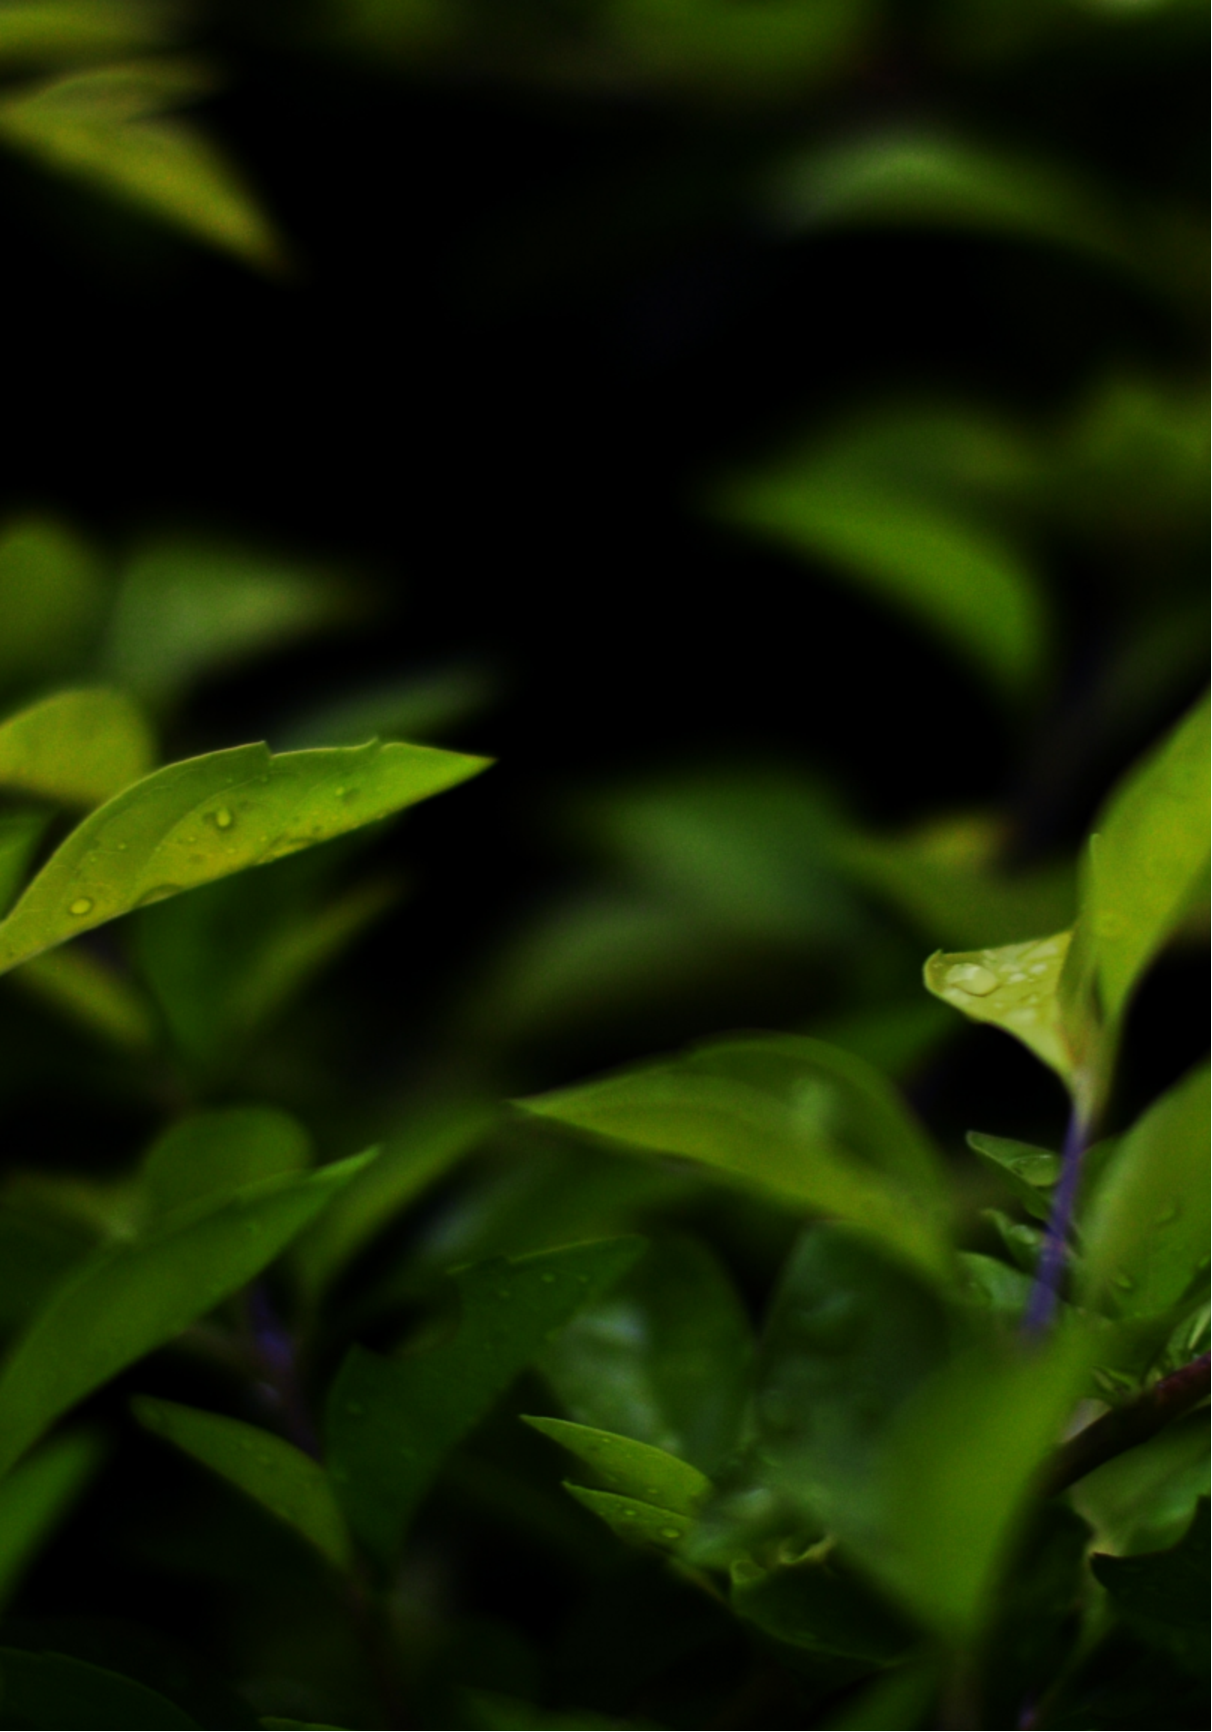
\includegraphics[width=\paperwidth]{background}}; % Background image
\draw[anchor=north] (midpoint) node 
[fill=ocre!30!white,fill opacity=0.6,text opacity=1,inner sep=1cm]
{\Huge\centering\bfseries\sffamily\parbox[c][][t]{\paperwidth}
{\centering Métodos numéricos\\[15pt] % Book title
{\Large Handbook}\\[20pt] % Subtitle
{\huge Fernando Pujaico Rivera}}}; % Author name
\end{tikzpicture}};
\end{tikzpicture}
\vfill
\endgroup

%----------------------------------------------------------------------------------------
%	COPYRIGHT PAGE
%----------------------------------------------------------------------------------------

\newpage
~\vfill
\thispagestyle{empty}

\noindent Copyright \copyright\ 2019 Fernando Pujaico Rivera\\ % Copyright notice

\noindent \textsc{Publicado por Virtual Books}\\ % Publisher

\noindent \textsc{book-website.com}\\ % URL

\noindent Esta obra está licenciada com uma Licença Creative Commons 
Atribuição-NãoComercial-CompartilhaIgual 4.0 Internacional. 
Não é possível usar este arquivo excepto em conformidade com a Licença. 
Pode obter uma copia de la Licença em
\url{http://creativecommons.org/licenses/by-nc-sa/4.0/}.\\ % License information

\noindent \textit{Primeira impressão , Março 2019} % Printing/edition date


%----------------------------------------------------------------------------------------
%	DEDICATORIA
%----------------------------------------------------------------------------------------

\cleardoublepage

\null
\vfill
\thispagestyle{empty}



{\normalsize \it \hfill Amicum lege feliciter, vivas, gaudeas, floreas in Deo. \vspace*{4pt}

%\hfill understanding and assistance they have given me. \vspace*{4pt}

\hfill Fernando \vspace*{4pt}}

 


%----------------------------------------------------------------------------------------
%	Acknowledgements
%----------------------------------------------------------------------------------------

\cleardoublepage

\begin{center}
\Huge{\textbf{Agradecimentos}}
\end{center}

\null
\vfill
\thispagestyle{empty}

{\normalsize \it \hfill Dou muitas graças a Deus \vspace*{4pt}}


~\\

{\normalsize \it Dou muitas graças a XXXXX XXXXXXXXX por me 
ajudar a corrigir muitos dos erros na escrita do livro.
\vspace*{4pt}}

{\normalsize \it Dou muitas graças a XXXXX XXXXXXXXX por me 
ajudar a revisar a forma da escrita na linguagem matemática do livro.
\vspace*{4pt}}

\begin{comment}
{\normalsize \it Dou muitas graças a XXXXX XXXXXXXXX por me 
ajudar a resolver muitas duvidas sobre definições e uso de termos na XXXXXXX XXXXXXX.
\vspace*{4pt}}
\end{comment}

\begin{comment}
{\normalsize \it Dou muitas graças a XXXXX XXXXXXXXX pela 
suas sugestões e revisão  do capitulo XXXXX XXXXXXXXX.
\vspace*{4pt}}
\end{comment}


 


%----------------------------------------------------------------------------------------
%	My macros
%----------------------------------------------------------------------------------------
%% diagonal function
\newcommand{\funcdiag}{diag}


%% vectorization function
\newcommand{\funcvec}{vec}

%% transpose function
\newcommand{\functrans}{trans}
%% transpose operator
\newcommand{\transpose}{\mathrm{T}}

%% block matrix
\newcommand{\funcblockdiag}{blkdiag}
\newcommand{\funcblockhor }{blkhorz}
\newcommand{\funcblockver }{blkvert}




%----------------------------------------------------------------------------------------
%	TABLE OF CONTENTS
%----------------------------------------------------------------------------------------

\chapterimage{chapter_head_1.pdf} % Table of contents heading image

\pagestyle{empty} % No headers

\renewcommand*\contentsname{Conteúdo}
\tableofcontents % Print the table of contents itself

%%%%%%%%%%%%%%%%%%%%%%%%%%%%%%%%%%%%%%%%%%%%%%%%%%%%%%%%%%%%%%%%%%%%%%%%%%%%%%%%
%%%%%%%%%%%%%%%%%%%%%%%%%%%%%%%%%%%%%%%%%%%%%%%%%%%%%%%%%%%%%%%%%%%%%%%%%%%%%%%%
%%%%%%%%%%%%%%%%%%%%%%%%%%%%%%%%%%%%%%%%%%%%%%%%%%%%%%%%%%%%%%%%%%%%%%%%%%%%%%%%
%% Lista de figuras (gerada automaticamente)
\cleardoublepage
\renewcommand*\listfigurename{Lista de figuras}
%\addcontentsline{toc}{chapter}{Lista de Figuras}
\listoffigures

%% Lista de tabelas (gerada automaticamente)
\cleardoublepage
%\addcontentsline{toc}{chapter}{Lista de Tablas}
\renewcommand*\listtablename{Lista de tabelas}
\listoftables

%% Glossário (gerado automaticamente)
\cleardoublepage
%\renewcommand{\nomname}{Glossary}
%\addcontentsline{toc}{chapter}{\nomname}
%\markboth{GLOSSARY}{GLOSSARY}
\printnomenclature

%%% Lista de Simbolos (gerada manualmente)
\cleardoublepage
\addcontentsline{toc}{chapter}{Lista de símbolos}
%%\markboth{LIST OF SYMBOLS}{LIST OF SYMBOLS}
\chapter*{Lista de Símbolos}

\singlespacing

%\noindent
\section*{Tipos de Dados}
\begin{tabular}{r | p{.45\linewidth} | l}
\hline	
Tipo & Descrição & Formatação \\ \hline
$\mathbf{A}$, $\mathbf{B}$, ..., $\mathbf{X}$, $\mathbf{Y}$, $\mathbf{Z}$& Matriz. & Maiúsculo e negrito \\
$\mathbf{a}$, $\mathbf{b}$, ..., $\mathbf{x}$, $\mathbf{y}$, $\mathbf{z}$ & Vetor (Por falta é asumido que é um vetor coluna) ou conjunto. & Minúsculo e negrito \\
%$A$, $B$, ..., $X$, $Y$, $Z$ & ------- & Maiúsculo \\
$a$, $b$, ..., $x$, $y$, $z$ & Escalar variável. & Minúsculo \\
$A$, $B$, ..., $X$, $Y$, $Z$ & Escalar constante. & Minúsculo \\
$\alpha$, $\beta$, ..., $\chi$, $\psi$, $\omega$ & Escalar variável ou constante. & Letras gregas e minúsculo  \\ \hline
\end{tabular}

\section*{Elementos de matrizes bidimensionais}
\begin{tabular}{r | p{.55\linewidth} | l}
\hline	
Tipo & Descrição & Formatação \\ \hline
$a_{ij}$ & Escalar formado pelo elemento da linha $i$, coluna $j$ da matriz $\mathbf{A}$. & Minúsculo \\ \hline
%$\mathbf{A}_{(i,j)}$& Elemento na linha $i$, coluna $j$ da matriz $\mathbf{A}$ & Maiúsculo e negrito \\ \hline
%$\mathbf{a}_{i}$ & Linha ou coluna $i$-essima da matriz $\mathbf{A}$ (ambíguo) & Minúsculo e negrito \\
$a_{i:}$ & Vetor linha formado pela linha $i$-essima da matriz $\mathbf{A}$.  & Minúsculo \\
%$\mathbf{A}_{(i,:)}$& Vetor formado pela linha $i$-essima da matriz $\mathbf{A}$ & Maiúsculo e negrito \\
$a_{:i}$ & Vetor coluna formado pela coluna $i$-essima da matriz $\mathbf{A}$.  & Minúsculo \\
%$\mathbf{A}_{(:,i)}$& Vetor formado pela coluna $i$-essima da matriz $\mathbf{A}$ & Maiúsculo e negrito \\ \hline
\end{tabular}

\section*{Elementos de vetores ou conjuntos}
\begin{tabular}{r | p{.55\linewidth} | l}
\hline	
Tipo & Descrição & Formatação \\ \hline
$a_{i}$ & Elemento $i$-essimo do vetor ou conjunto  $\mathbf{a}$.& Minúsculo \\
%$\mathbf{a}_{(i)}$ & Elemento $i$-essimo do vetor $\mathbf{a}$ & Minúsculo e negrito \\ \hline
\end{tabular}

\section*{Funções notáveis}
\begin{tabular}{r | p{.70\linewidth} }
\hline	
Função & Descrição \\ \hline
$card(\mathbf{a})$ & Número de elementos, cardinalidade, do vetor ou conjunto $\mathbf{a}$. \\
$card(\mathbf{A})$ & Número de elementos, cardinalidade, da matriz $\mathbf{A}$. \\
\hline
$dim(\mathbf{a},1)$ & Primeira dimensão do vetor $\mathbf{a}$, número de linhas. \\
$dim(\mathbf{a},2)$ & Segunda dimensão do vetor $\mathbf{a}$, número de colunas. \\
$dim(\mathbf{A},1)$ & Primeira dimensão da matriz $\mathbf{A}$, número de linhas. \\
$dim(\mathbf{A},2)$ & Segunda dimensão da matriz $\mathbf{A}$, número de colunas. \\
$dim(\mathbf{A},N)$ & Dimensão $N$ da matriz $\mathbf{A}$, se não tiver retorna $0$. \\
\hline
$inv(\mathbf{A})$ & Inversa da matriz $\mathbf{A}$, é equivalente a escrever $\mathbf{A}^{-1}$. \\
$\mathbf{A}^{-1}$ & Inversa da matriz $\mathbf{A}$, é equivalente a escrever $inv(\mathbf{A})$. \\
\hline
$trans(\mathbf{a})$ & Transposta do vetor $\mathbf{a}$, é equivalente a escrever $\mathbf{a}^{T}$. \\
$\mathbf{a}^{T}$ & Transposta do vetor $\mathbf{a}$, é equivalente a escrever $trans(\mathbf{a})$. \\
$trans(\mathbf{A})$ & Transposta da matriz $\mathbf{A}$, é equivalente a escrever $\mathbf{A}^{T}$. \\
$\mathbf{A}^{T}$ & Transposta da matriz $\mathbf{A}$, é equivalente a escrever $trans(\mathbf{A})$. \\
\hline
$||\mathbf{a}||$ & Módulo do vetor $\mathbf{a}$, é equivalente a escrever $\sqrt{\sum_i a_i^2}$. \\
$||\mathbf{a}||^2$ & Módulo ao quadrado do vetor $\mathbf{a}$, 
é equivalente a escrever $\sum_i a_i^2$ ou $\mathbf{a}^{T}\mathbf{a}$ se $\mathbf{a}$ é um vetor coluna. \\
$||\mathbf{a}||_{\mathbf{B}}^2$ & Módulo ao quadrado ponderado do vetor $\mathbf{a}$, 
é equivalente a escrever $\sum_i b_{ii} a_i^2$ ou $(\sqrt{\mathbf{B}}~\mathbf{a})^{T}\sqrt{\mathbf{B}}~\mathbf{a} \equiv \mathbf{a}^{T}\mathbf{B}\mathbf{a}$ 
se $\mathbf{a}$ é um vetor coluna. Sendo que $\mathbf{B}$ é uma matriz diagonal.\\
\end{tabular}

\onehalfspacing

%%%%%%%%%%%%%%%%%%%%%%%%%%%%%%%%%%%%%%%%%%%%%%%%%%%%%%%%%%%%%%%%%%%%%%%%%%%%%%%%
%%%%%%%%%%%%%%%%%%%%%%%%%%%%%%%%%%%%%%%%%%%%%%%%%%%%%%%%%%%%%%%%%%%%%%%%%%%%%%%%


\cleardoublepage % Forces the first chapter to start on an odd page so it's on the right

\pagestyle{fancy} % Print headers again

%----------------------------------------------------------------------------------------
%	PART
%----------------------------------------------------------------------------------------

\part{Derivadas de funções e operadores}
%\chapterimage{chapter_letras.pdf} % Chapter heading image

\chapter{Notações e termos}

%%%%%%%%%%%%%%%%%%%%%%%%%%%%%%%%%%%%%%%%%%%%%%%%%%%%%%%%%%%%%%%%%%%%%%%%%%%%%%%%
%%%%%%%%%%%%%%%%%%%%%%%%%%%%%%%%%%%%%%%%%%%%%%%%%%%%%%%%%%%%%%%%%%%%%%%%%%%%%%%%
%%%%%%%%%%%%%%%%%%%%%%%%%%%%%%%%%%%%%%%%%%%%%%%%%%%%%%%%%%%%%%%%%%%%%%%%%%%%%%%%
\section{Notação usada para matrizes, vetores e funções}
\begin{notation}[Modo em que os valores escalares, vetoriais ou matriciais são definidos:]~\\
\begin{tabular}{p{.2\textwidth} | p{.4\textwidth} | p{.3\textwidth} }
\hline	
\textbf{Tipo} & \textbf{Descrição} & \textbf{Formatação} \\ \hline
$\MATRIX{A}$, $\MATRIX{B}$, ..., $\MATRIX{X}$, $\MATRIX{Y}$, $\MATRIX{Z}$& Matriz. & Maiúsculo e negrito \\
$\VECTOR{a}$, $\VECTOR{b}$, ..., $\VECTOR{x}$, $\VECTOR{y}$, $\VECTOR{z}$ & Vetor ou conjunto. & Minúsculo e negrito \\
%$A$, $B$, ..., $X$, $Y$, $Z$ & ------- & Maiúsculo \\
$a$, $b$, ..., $x$, $y$, $z$ & Escalar variável. & Minúsculo \\
$A$, $B$, ..., $X$, $Y$, $Z$ & Escalar constante. & Maiúsculo \\
$\alpha$, $\beta$, ..., $\chi$, $\psi$, $\omega$ & Escalar variável ou constante. & Letras gregas  \\ \hline
\end{tabular}
\end{notation}


\begin{notation}[Funções notáveis usadas neste livro:]~\\
\begin{tabular}{p{.11\textwidth} |  p{.8\textwidth} }
\hline	
\textbf{Função} & \textbf{Descrição} \\ \hline
%$card(\VECTOR{a})$ & Número de elementos, cardinalidade, do vetor ou conjunto $\VECTOR{a}$. \\
$card(\MATRIX{A})$ & Número de elementos, cardinalidade, da matriz $\MATRIX{A}$. \\
\hline
%$dim(\VECTOR{a},1)$ & Primeira dimensão do vetor $\VECTOR{a}$, número de linhas. \\
%$dim(\VECTOR{a},2)$ & Segunda dimensão do vetor $\VECTOR{a}$, número de colunas. \\
$dim(\MATRIX{A},1)$ & Primeira dimensão da matriz $\MATRIX{A}$, número de linhas. \\
$dim(\MATRIX{A},2)$ & Segunda dimensão da matriz $\MATRIX{A}$, número de colunas. \\
$dim(\MATRIX{A},N)$ & Dimensão $N$ da matriz $\MATRIX{A}$, se não tiver retorna $1$. \\
\hline
$\funcinv(\MATRIX{A})$ & Inversa da matriz $\MATRIX{A}$, é equivalente a escrever $\MATRIX{A}^{-1}$. \\
$\MATRIX{A}^{-1}$ & Inversa da matriz $\MATRIX{A}$, é equivalente a escrever $\funcinv(\MATRIX{A})$. \\
\hline
%$\functrans(\VECTOR{a})$ & Transposta do vetor $\VECTOR{a}$, é equivalente a escrever $\VECTOR{a}^{\transpose}$. \\
%$\VECTOR{a}^{\transpose}$ & Transposta do vetor $\VECTOR{a}$, é equivalente a escrever $trans(\VECTOR{a})$. \\
$\functrans(\MATRIX{A})$ & Transposta da matriz $\MATRIX{A}$, é equivalente a escrever $\MATRIX{A}^{\transpose}$. \\
$\MATRIX{A}^{\transpose}$ & Transposta da matriz $\MATRIX{A}$, é equivalente a escrever $trans(\MATRIX{A})$. \\
\hline
$\funcdiag(\VECTOR{a})$ & Matriz diagonal construída a partir de colocar na diagonal os elementos do vetor $\VECTOR{a}$ . \\
\hline
$\lambda_{\MATRIX{A}}$ & Matriz diagonal onde os elementos da diagonal correspondem com os autovalores da matriz $\MATRIX{A}$. \\
\hline
$det(\MATRIX{A})$ & Determinante da matriz $\MATRIX{A}$. \\
\hline
\end{tabular}
\end{notation}

\newpage
\begin{notation}[Modo em que os elementos dos vetores ou conjuntos são definidos:]
\begin{tabular}{p{.05\textwidth} | p{.6\textwidth} | p{.25\textwidth}}
\hline	
\textbf{Tipo} & \textbf{Descrição} & \textbf{Formatação} \\ \hline
$a_{i}$ & Elemento $i$-ésimo do vetor ou conjunto  $\VECTOR{a}$.& Minúsculo \\
%$\VECTOR{a}_{(i)}$ & Elemento $i$-ésimo do vetor $\VECTOR{a}$ & Minúsculo e negrito \\ \hline
\hline
\end{tabular}
\end{notation}


\begin{notation}[Modo em que os elementos das matrizes bidimensionais são definidos:]~\\
\begin{tabular}{p{.05\textwidth} | p{.6\textwidth} | p{.25\textwidth}}
\hline	
\textbf{Tipo} & \textbf{Descrição} & \textbf{Formatação} \\ \hline
$a_{ij}$ & Escalar formado pelo elemento na linha $i$, coluna $j$ da matriz $\MATRIX{A}$. & Minúsculo \\ \hline
%$\MATRIX{A}_{(i,j)}$& Elemento na linha $i$, coluna $j$ da matriz $\MATRIX{A}$ & Maiúsculo e negrito \\ \hline
%$\VECTOR{a}_{i}$ & Linha ou coluna $i$-ésima da matriz $\MATRIX{A}$ (ambíguo) & Minúsculo e negrito \\
$a_{i:}$ & Vetor linha formado pela linha $i$-ésima da matriz $\MATRIX{A}$.  & Minúsculo \\
%$\MATRIX{A}_{(i,:)}$& Vetor formado pela linha $i$-ésima da matriz $\MATRIX{A}$ & Maiúsculo e negrito \\
$a_{:i}$ & Vetor coluna formado pela coluna $i$-ésima da matriz $\MATRIX{A}$.  & Minúsculo \\
%$\MATRIX{A}_{(:,i)}$& Vetor formado pela coluna $i$-ésima da matriz $\MATRIX{A}$ & Maiúsculo e negrito \\ \hline
\hline
\end{tabular}
\end{notation}


\begin{notation}[Funções em tempo continuo e discreto:]~\\
\begin{tabular}{p{.05\textwidth} | p{.85\textwidth} }
\hline	
\textbf{Tipo}            & \textbf{Descrição} \\ \hline
$x(t)$          & Função escalar de domínio continuo, representado pela variável $t$. \\ \hline
$x[n]$          & Função escalar de domínio discreto, onde a variável $n$ representa a $n$-ésima amostra. \\ \hline
$\VECTOR{x}(t)$ & Função vetorial de domínio continuo, representado pela variável $t$.  \\ \hline
$\VECTOR{x}[n]$ & Função vetorial de domínio discreto, onde a variável $n$ representa a $n$-ésima amostra. \\
\hline
\end{tabular}
\end{notation}



%%%%%%%%%%%%%%%%%%%%%%%%%%%%%%%%%%%%%%%%%%%%%%%%%%%%%%%%%%%%%%%%%%%%%%%%%%%%%%%%
%%%%%%%%%%%%%%%%%%%%%%%%%%%%%%%%%%%%%%%%%%%%%%%%%%%%%%%%%%%%%%%%%%%%%%%%%%%%%%%%
%%%%%%%%%%%%%%%%%%%%%%%%%%%%%%%%%%%%%%%%%%%%%%%%%%%%%%%%%%%%%%%%%%%%%%%%%%%%%%%%
\section{A linguagem matemática}

\begin{description}

\item[Definição:] \index{Definição} Uma definição é uma declaração na qual as pessoas interessadas chegam a um acordo \cite[pp. 37]{solow1987como}.
Se a definição não é aceita é impossível a comunicação de temas relacionados à definição.
\begin{example}[Uso de termos em triângulos:]~\\
\begin{itemize}
\item \textbf{Definição:} Um triângulo é chamado isósceles se dois do seus lados são iguais.
\item \textbf{Definição:} Um triângulo é chamado retângulo se tem um ângulo com $90^{\circ}$.
\item \textbf{Definição:} Um angulo é chamado reto se tem  $90^{\circ}$.
\end{itemize}
\end{example}

\item[Axioma ou Postulado:] \index{Axioma} \index{Postulado} 
Uma proposição que é aceita sem uma demostração formal \cite[pp. 47]{fossa2009introducao} \cite[pp. 41]{solow1987como}.
\begin{example}[Sobre os ângulos num triângulo isósceles:]~\\
\begin{itemize}
\item \textbf{Quinto Postulado de Euclides:} Se uma reta cortar duas outras retas de modo que a soma dos dois ângulos interiores, de um mesmo lado, seja menor que dois ângulos retos, então as duas outras retas se cruzam, quando suficientemente prolongadas, do lado da primeira reta em que se acham os dois ângulos.
\end{itemize}
\end{example}

Antigamente existia uma distinção mais acentuada entre os termos axioma e postulado \cite[pp. 115]{de1863ensaio},
porém o uso popular foi acurtando a distancia entre estes dois termos \cite[pp. 243]{mora2000dicionario}.
Por exemplo, nesse antigo uso dos termos axioma e postulado, poderíamos entender estos termos como,
\begin{itemize}
\item \textbf{Axioma:} ``Isto é assim porque é evidente, não preciso demostrar''.
\item \textbf{Postulado:} ``Para futuras interações gostaria propor que partamos da base que esta afirmação é verdadeira,
 para poder chegar a conclusões decorrentes desta afirmação em nosso dialogo''.
\end{itemize}


\item[Lema:] \index{Lema} Um lema é uma proposição preliminar demostrada, 
a qual será usada para demostrar um teorema \cite[pp. 49]{fossa2009introducao}\cite[pp. 41]{solow1987como},
a afirmação indicada pelo lema não tem muita importância matemática em sim mesma, mas cumpre um papel importante para a demostração de um teorema.
Falando de forma estrita um lema também é um teorema; é dizer, uma proposição demostrada.
\begin{example}[Sobre os ângulos num triângulo isósceles:]~\\
\begin{itemize}
\item \textbf{Lema:} Num triangulo, se um angulo é reto os outros dois somam $90^{\circ}$.
\end{itemize}
\end{example}

\item[Proposição:] \index{Proposição} Uma proposição é um enunciado ou afirmação que se busca demostrar \cite[pp. 41]{solow1987como}.
\begin{example}[Sobre os ângulos num triângulo isósceles:]~\\
\begin{itemize}
\item \textbf{Proposição:} Num triangulo isósceles, uma linha que parte do vértice com lados iguais e divide ao lado oposto na metade,
forma um ângulo reto com este lado.
\end{itemize}
\end{example}

\item[Teorema:] \index{Teorema} Um teorema é uma proposição demostrada \cite[pp. 49]{fossa2009introducao} \cite[pp. 41]{solow1987como}.
\begin{example}[Sobre os ângulos num triângulo isósceles:]~\\
\begin{itemize}
\item \textbf{Teorema:} Num triangulo isósceles, uma linha que parte do vértice com lados iguais e divide ao lado oposto na metade,
forma um ângulo reto com este lado.
\item \textbf{Prova:}  Se chamamos $2\beta$ ao ângulo entre os lados iguais, 
e $\alpha$ a cada um dos ângulos restantes do triângulo isósceles. Sabendo
que a soma de ângulos num triângulo é $180^{\circ}=2\beta+2\alpha$,
concluímos que $\beta+\alpha=90^{\circ}$.
Dado que cada um dos dois triângulos formados pela divisão criada pela linha, tem ângulos $\alpha$ e $\beta$,
podemos concluir que o ângulo restante tem $90^{\circ}$, é dizer é um ângulo reto.
\end{itemize}
\end{example}

\item[Corolário:] \index{Corolário} Um corolário é uma proposição 
fácil de demostrar que se deduz a partir de um teorema \cite[pp. 49]{fossa2009introducao} \cite[pp. 41]{solow1987como}.
Falando de forma estrita um corolário também é um teorema; é dizer, uma proposição demostrada.
\begin{example}[Sobre os ângulos num triângulo isósceles:]~\\
\begin{itemize}
\item \textbf{Corolário:} Num triangulo isósceles, 
uma linha que parte do vértice com lados iguais e divide ao lado oposto na metade,
cria dois triângulos retângulos.
\end{itemize}
\end{example}

\end{description}


%%%%%%%%%%%%%%%%%%%%%%%%%%%%%%%%%%%%%%%%%%%%%%%%%%%%%%%%%%%%%%%%%%%%%%%%%%%%%%%%
%%%%%%%%%%%%%%%%%%%%%%%%%%%%%%%%%%%%%%%%%%%%%%%%%%%%%%%%%%%%%%%%%%%%%%%%%%%%%%%%
%%%%%%%%%%%%%%%%%%%%%%%%%%%%%%%%%%%%%%%%%%%%%%%%%%%%%%%%%%%%%%%%%%%%%%%%%%%%%%%%
\section{Descrição geral do problema inverso}

\index{Problema!Direto}
\index{Problema!Inverso}
Segundo o matemático Joseph B. Keller \cite{Keller76}, dois problemas são considerados inversos 
um do outro, se a formulação de cada um deles envolve a resposta do outro,
de modo que por motivos históricos, um deles é bem conhecido e estudado,
pelo que recebe o nome de \textbf{problema direto}, 
e o outro problema é novo e pouco estudado, pelo que é chamado \textbf{problema inverso}.
 
\begin{example}[Raízes e polinômios:]~
\begin{description}
\item[Problema direto -] Achar as raízes $x_{z_1}$, $x_{z_2}$, ..., $x_{z_N}$, 
conhecendo os coeficientes do polinômio $p_{\VECTOR{c}}(x)$ agrupados no vetor $\VECTOR{c}$  \cite{Keller76}.
\item[Problema inverso -] Achar os coeficientes do polinômio $p_{\VECTOR{c}}(x)$ agrupados no vetor $\VECTOR{c}$, 
conhecendo que existem raízes em $x_{z_1}$, $x_{z_2}$, ..., $x_{z_N}$ \cite{Keller76}.
\end{description}
Uma representação gráfica do problema direto pode ser vista na Figura \ref{fig:inverso-diretos:direto1}
e do problema inverso na Figura \ref{fig:inverso-diretos:inverso1};
nesses exemplos não usamos entrada de dados, 
os coeficientes do polinômio agrupados no vetor $\VECTOR{c}$ são os parâmetros do sistema e 
os valores $x_{z_n}$ pertencem aos dados de saída.
\end{example}

\begin{example}[Avaliação vs. regressão:]~
\begin{description}
\item[Problema direto -] Achar os valores $y_1$,~ $y_2$,~ ...,~ $y_N$, 
conhecendo os coeficientes do polinômio $y=p_{\VECTOR{c}}(x)$, agrupados no vetor $\VECTOR{c}$, e
os valores $x_1$, $x_2$, ..., $x_N$ \cite{Keller76}.
\item[Problema inverso -] Achar os coeficientes do polinômio $y=p_{\VECTOR{c}}(x)$ agrupados no vetor $\VECTOR{c}$, 
conhecendo que existem os valores $x_1$, $x_2$, ..., $x_N$ e 
$y_1$,~ $y_2$,~ ...,~ $y_N$  \cite{Keller76}.
\end{description}
Uma representação gráfica do problema direto pode ser visto na Figura \ref{fig:inverso-diretos:direto1}
e do problema inverso na Figura \ref{fig:inverso-diretos:inverso1}, 
em que $x_n$ pertence à entrada de dados, 
os coeficientes do polinômio agrupados no vetor $\VECTOR{c}$ são os parâmetros 
do sistema, e $y_n$ pertence aos dados de saída.
\end{example}


\begin{example}[Avaliação vs. regressão:]~
\begin{description}
\item[Problema direto -] Achar os valores $y_1$, $y_2$, ..., $y_n$, ..., $y_N$, 
que são as respostas de avaliar um valor $x$ nos polinômios 
$y=p_{\VECTOR{c}_n}(x)$ com coeficientes agrupados em vetores $\VECTOR{c}_n$ \cite{Keller76}.
\item[Problema inverso -] Achar o valor $x$
conhecendo vários polinômios $y=p_{\VECTOR{c}_n}(x)$ com coeficientes agrupados em vetores $\VECTOR{c}_n$ e
os resultados $y_1$, $y_2$, ..., $y_n$, ..., $y_N$  \cite{Keller76}.
\end{description}
Uma representação gráfica do problema direto pode ser vista na Figura \ref{fig:inverso-diretos:direto1}
e do problema inverso na Figura \ref{fig:inverso-diretos:inverso2}.
\end{example}

\begin{figure}[!h]
     \centering
     \begin{subfigure}[b]{0.49\textwidth}
         \centering
         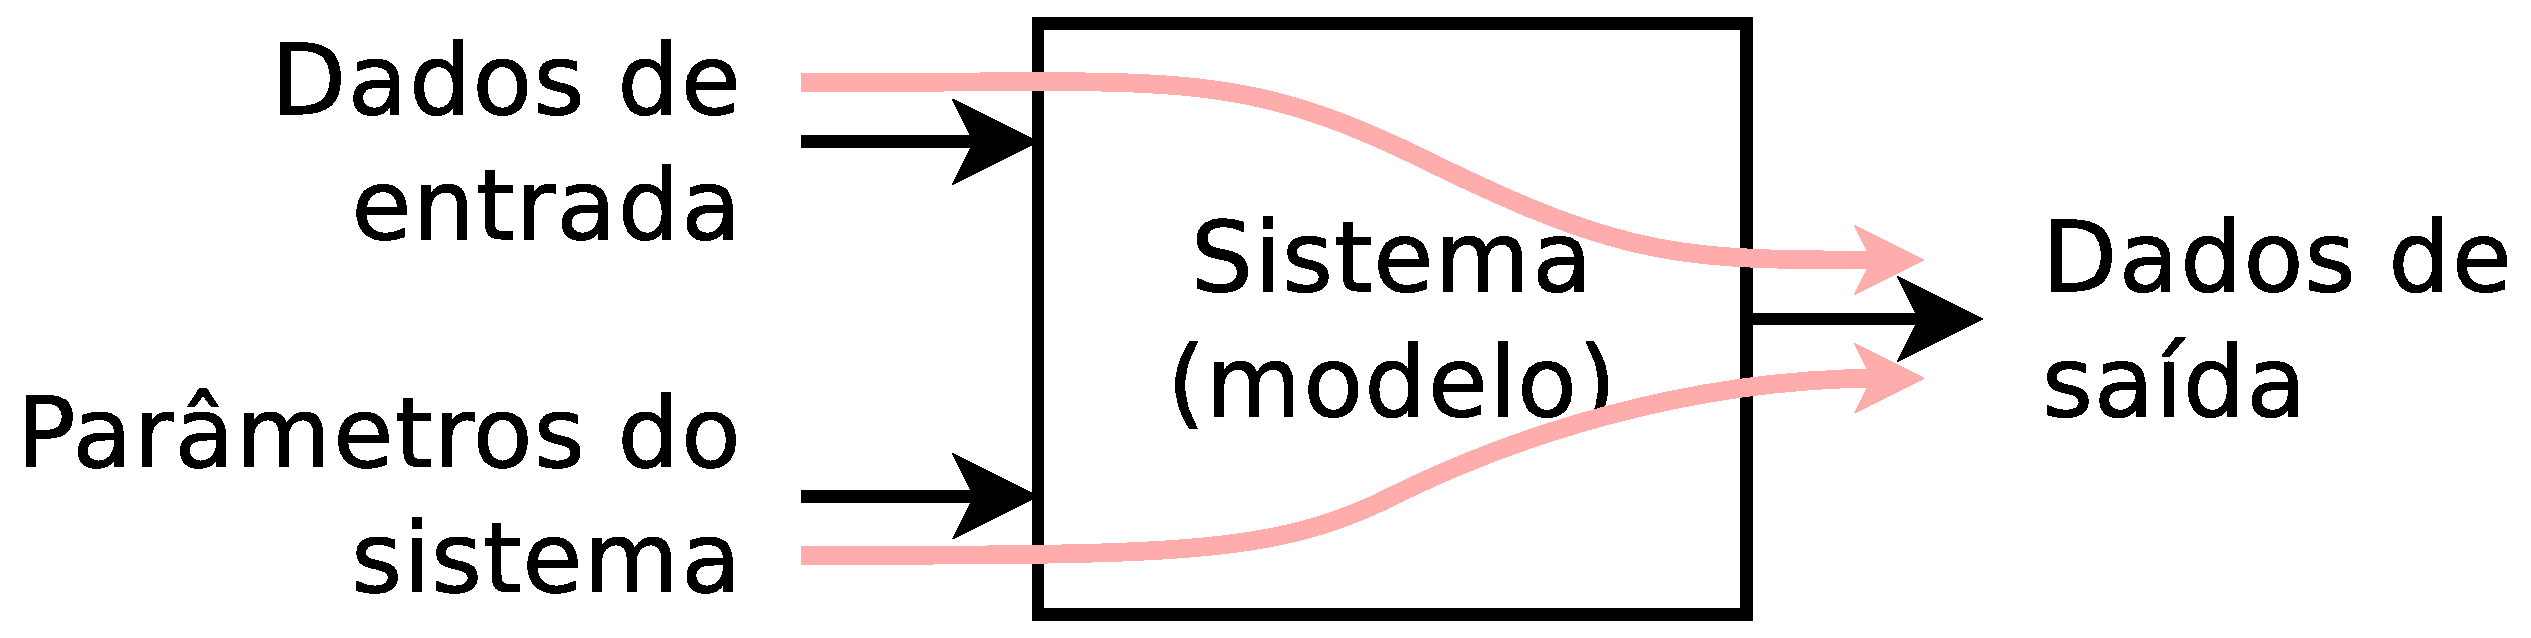
\includegraphics[width=0.95\textwidth]{chapters/notacao/direto1.eps}
         \caption{Problema direto.}
         \label{fig:inverso-diretos:direto1}
     \end{subfigure}
     \hfill
     \begin{subfigure}[b]{0.49\textwidth}
         \centering
         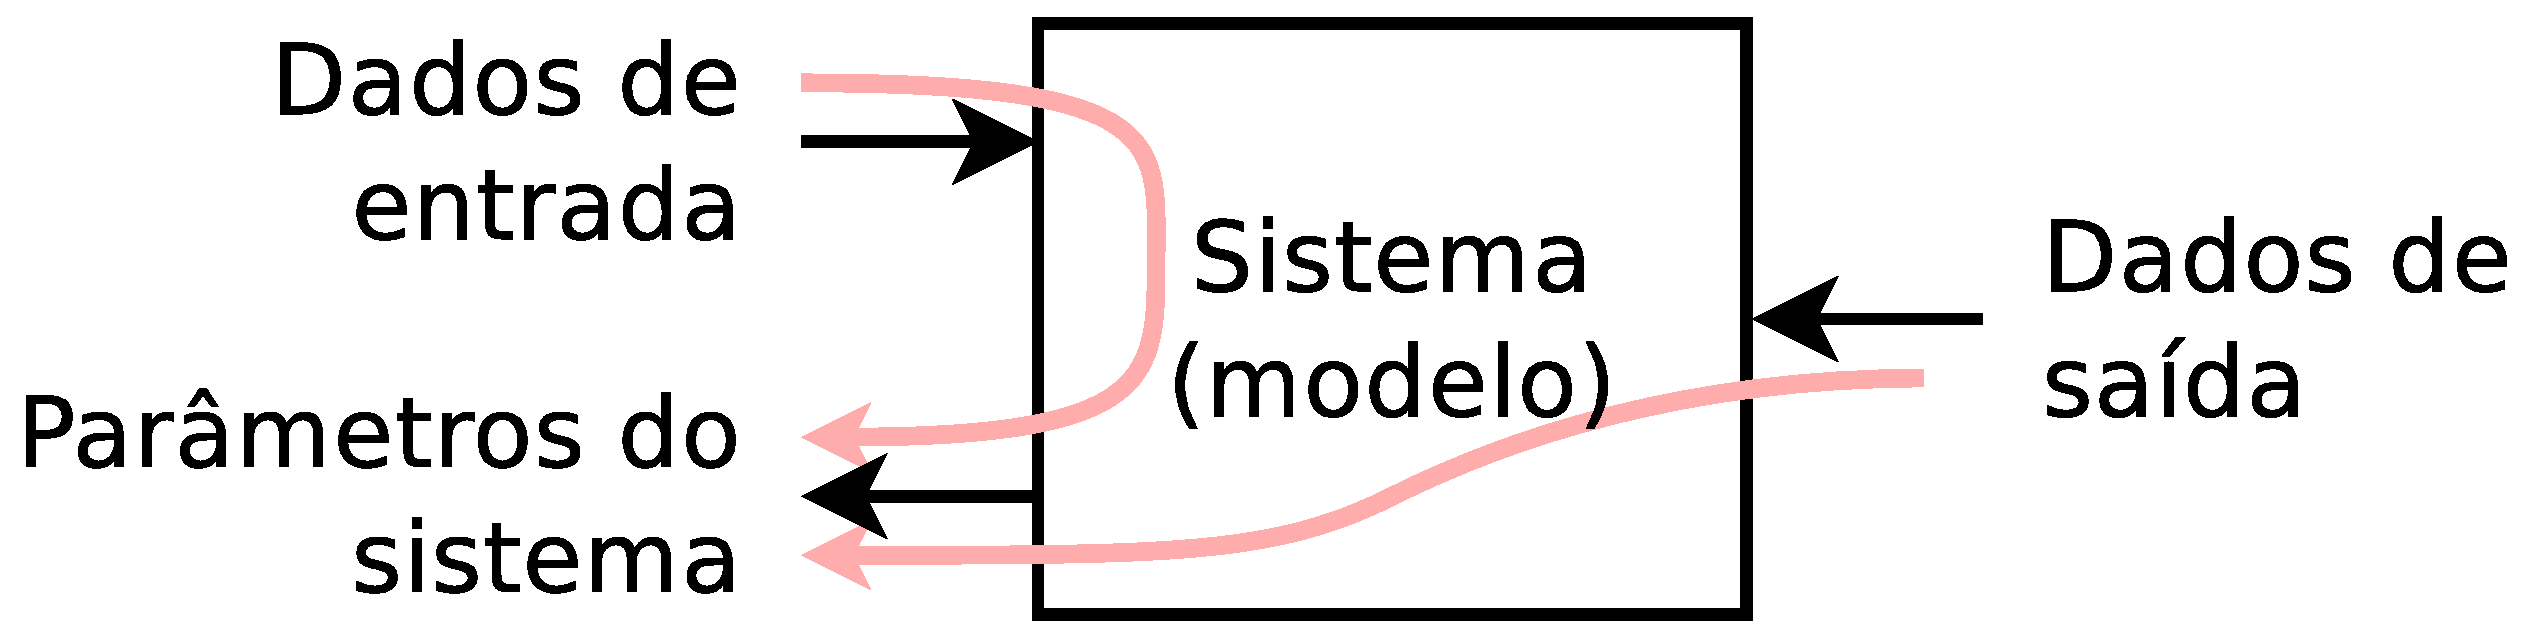
\includegraphics[width=0.95\textwidth]{chapters/notacao/inverso1.eps}
         \caption{Problema inverso.}
         \label{fig:inverso-diretos:inverso1}
     \end{subfigure}
     \hfill
     \begin{subfigure}[b]{0.49\textwidth}
         \centering
         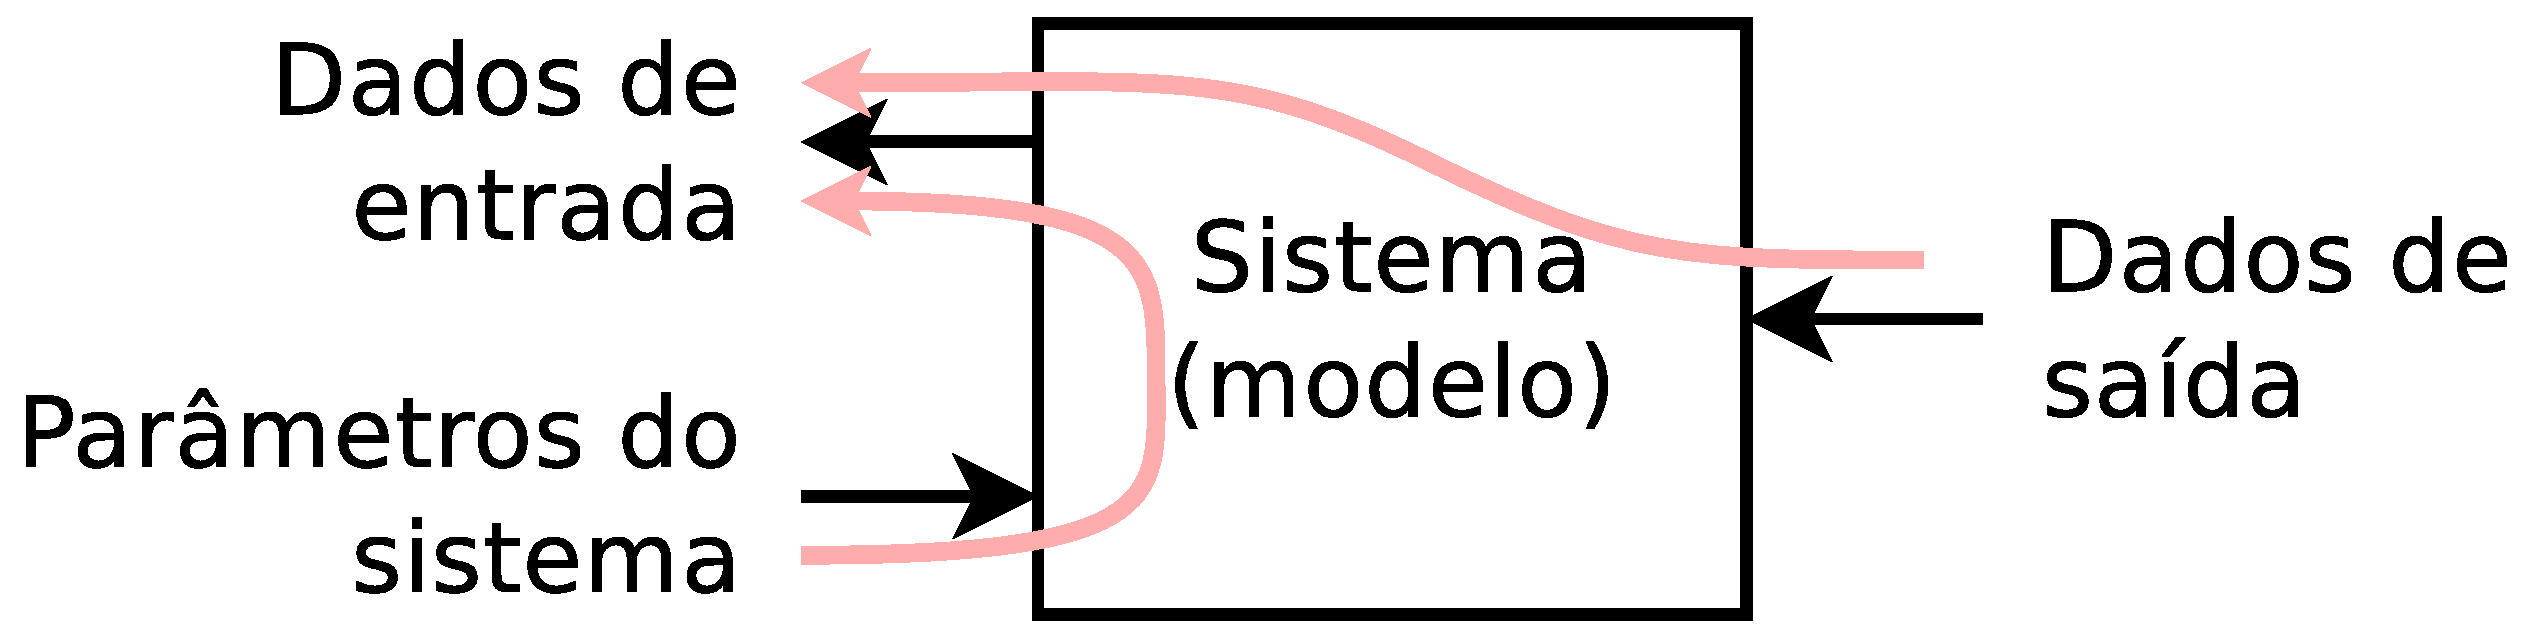
\includegraphics[width=0.95\textwidth]{chapters/notacao/inverso2.eps}
         \caption{Problema inverso.}
         \label{fig:inverso-diretos:inverso2}
     \end{subfigure}
        \caption{Exemplos de problemas diretos e inversos.}
        \label{fig:inverso-diretos}
\end{figure}


%%%%%%%%%%%%%%%%%%%%%%%%%%%%%%%%%%%%%%%%%%%%%%%%%%%%%%%%%%%%%%%%%%%%%%%%%%%%%%%%
%%%%%%%%%%%%%%%%%%%%%%%%%%%%%%%%%%%%%%%%%%%%%%%%%%%%%%%%%%%%%%%%%%%%%%%%%%%%%%%%
%%%%%%%%%%%%%%%%%%%%%%%%%%%%%%%%%%%%%%%%%%%%%%%%%%%%%%%%%%%%%%%%%%%%%%%%%%%%%%%%
\section{Problema \wellposed~ vs. \illposed }

%%%%%%%%%%%%%%%%%%%%%%%%%%%%%%%%%%%%%%%%%%%%%%%%%%%%%%%%%%%%%%%%%%%%%%%%%%%%%%%%
\subsection{Problema \wellposed}
\index{Problema!\Wellposed}
\index{Well-posed}
\begin{definition}[Problema \wellposed:]
\label{def:bem-posto:1}
Conhecido um modelo matemático ou sistema que desejamos manipular para obter uma solução;
indicamos que este é um problema \wellposed~ (do inglês ``well-posed'') 
quando se cumprem 3 condições\footnote{A primeira definição de um problema \wellposed~ foi realizada pelo matemático J. S. Hadamard, 
para mais detalhes sobre Hadamard ver a Pag. \pageref{elab:Hadamard}.} \cite[pp. 16]{gockenbach2016linear}
\cite[pp. 6]{p2011well}.
\begin{itemize}
\item \textbf{Existência:} Existe uma solução que verifica o sistema.
\item \textbf{Unicidade:} A solução é única.
\item \textbf{Estabilidade:} A solução depende continuamente da saída;
é dizer, pequenas variações na resposta provem de pequenas variações nos dados usados para calcular a resposta.
\end{itemize}
\end{definition}

\begin{example}[Problema \wellposed:]
Conhecido o problema de obter o vetor $\VECTOR{x} \in \mathbb{R}^{N}$,
que cumpre o sistema, $\MATRIX{A}\VECTOR{x}=\VECTOR{y}$,
 tendo como dados o vetor $\VECTOR{y} \in \mathbb{R}^{N}$ e 
a matriz $\MATRIX{A}: \mathbb{R}^{N} \rightarrow \mathbb{R}^{N}$ que carateriza ao sistema.
Falamos que o problema está \wellposed~ se a matriz $\MATRIX{A}$ tem inversa e esta é limitada \cite[pp. 18]{gockenbach2016linear}. 
\end{example}

%%%%%%%%%%%%%%%%%%%%%%%%%%%%%%%%%%%%%%%%%%%%%%%%%%%%%%%%%%%%%%%%%%%%%%%%%%%%%%%%
\subsection{Problema \illposed}
\index{Ill-posed}
\index{Problema!\Illposed}
\begin{definition}[Problema \illposed:]
\label{def:mal-posto:1}
Um problema é chamado \illposed~ (do inglês ``ill-posed'') se não cumpre um o mais das condições que definem a um problema 
\wellposed~ \cite[pp. 18]{gockenbach2016linear}.
Os problemas inversos geralmente são relacionados a um problema \illposed,
pois pelo geral não cumprem uma ou mais das condições para ser catalogados como \wellposed. 
\end{definition}

\begin{example}[Problema \illposed~ sem solução:]
\label{ex:IllPosedNoSolutions}
Conhecido o problema de obter o vetor $\VECTOR{x}\in \mathbb{R}^N$,
que cumpre o sistema,
\begin{equation}
\MATRIX{A}\VECTOR{x}=\VECTOR{y},
\qquad
\MATRIX{A}=
\begin{bmatrix}
1 & 1\\
2 & 1\\
0 & 1
\end{bmatrix}
\qquad
\VECTOR{y}=
\begin{bmatrix}
2\\
3\\
2
\end{bmatrix};
\end{equation}
catalogamos este problema como \illposed~ pois não existe um vetor $\VECTOR{x}$
que verifique o sistema $\MATRIX{A}\VECTOR{x}=\VECTOR{y}$.
\end{example}


\begin{example}[Problema \illposed~com múltiplas soluções:]
\label{ex:IllPosedMultiplaSolutions}
Conhecido o problema de obter o vetor $\VECTOR{x}\in \mathbb{R}^N$,
que cumpre o sistema,
\begin{equation}
\MATRIX{A}\VECTOR{x}=\VECTOR{y},
\qquad
\MATRIX{A}=
\begin{bmatrix}
1 & 1\\
1 & 1\\
1 & 1
\end{bmatrix}
\qquad
\VECTOR{y}=
\begin{bmatrix}
2\\
2\\
2
\end{bmatrix};
\end{equation}
catalogamos este problema como \illposed~  pois existem múltiplas soluções $\VECTOR{x}$
que cumprem o sistema,
$
\VECTOR{x}=
\begin{bmatrix}
2 & 0
\end{bmatrix}^{\transpose}
+\alpha
\begin{bmatrix}
-1 & 1
\end{bmatrix} ^{\transpose}$,
$ \forall \alpha \in \mathbb{R}$.
\end{example}

\index{Hadamard, Jacques Salomon}
\begin{elaboracion}[title=Jacques Salomon Hadamard (1865-1963), width= 0.99\linewidth]
\label{elab:Hadamard}
\noindent
\begin{minipage}{0.2\linewidth}
\centering
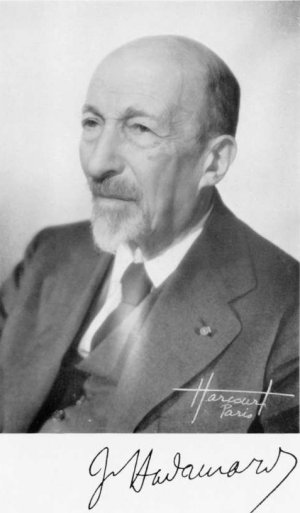
\includegraphics[width=0.98\textwidth]{chapters/notacao/Hadamard2.jpg}
\end{minipage}
\begin{minipage}{0.8\linewidth}
Notável matemático francês  e um membro da Royal Society;
durante seus primeiros anos de vida, 
Jacques se destacou em todas as disciplinas, exceto em matemática;
sua habilidade nesta área melhorou notavelmente após sua admissão no Lycée Louis-le-Grand em 1876;
logo de vários anos, cheios de  grandes realizações acadêmicas, ele completou seu Ph.D. em 1892 
e recebeu o prêmio Grand Prix de Ciências Matemáticas por seu ensaio inovador sobre a função zeta de Riemann
\cite[pp. 326]{agarwal2014creators}.
Entre suas muitas contribuições à matemática está a definição inicial de um problema \wellposed,
e consequentemente a de um problema \illposed~\cite[pp. 9, 132]{p2011well}.
\end{minipage}
\end{elaboracion}

\begin{comment}
\begin{tcbinformation} 
\textbf{Hadamard e os problemas \illposed:} 
O matemático Jacques Salomon Hadamard fez a definição inicial de um problema \wellposed,
e consequentemente a de um problema \illposed; 
ele  indicou como irrelevantes para a física ou para as aplicações do mundo real
a qualquer problema catalogado como \illposed; porém,
quatro décadas após sua declaração esta afirmação ele provou estar errado  \cite[pp. 4]{siddiqi2011mathematics}.
\end{tcbinformation} 
\end{comment}



%%%%%%%%%%%%%%%%%%%%%%%%%%%%%%%%%%%%%%%%%%%%%%%%%%%%%%%%%%%%%%%%%%%%%%%%%%%%%%%%
%%%%%%%%%%%%%%%%%%%%%%%%%%%%%%%%%%%%%%%%%%%%%%%%%%%%%%%%%%%%%%%%%%%%%%%%%%%%%%%%
%%%%%%%%%%%%%%%%%%%%%%%%%%%%%%%%%%%%%%%%%%%%%%%%%%%%%%%%%%%%%%%%%%%%%%%%%%%%%%%%
\section{Regularização}




A regularização é o processo pelo qual um problema \illposed~
é aproximado por uma família vizinha de problemas \wellposed~
\cite[pp. 49]{engl2000regularization},
para realizar esta aproximação, informação adicional é considerada no problema.


Assim, por exemplo, podemos aplicar a regularização agregando uma função objetivo para obter um problema de otimização.

\textbf{Problema direto:} Considere um sistema representado pelo seguinte problema direto,
\begin{equation}\label{eq:regularization:1}
\MATRIX{A}\VECTOR{x}=\VECTOR{y},
\end{equation}
onde a resposta vector $\VECTOR{y}\in \mathbb{R}^M$ é obtida logo de introduzir o estimulo $\VECTOR{x}\in \mathbb{R}^N$,
sendo $\MATRIX{A}:\mathbb{R}^N \rightarrow \mathbb{R}^M$ uma matriz operador lineal.

\textbf{Problema inverso:} Assim, o problema inverso para o sistema da Eq. (\ref{eq:regularization:1}), é
achar o vetor de entrada $\VECTOR{x}$, que cumpra  a Eq. (\ref{eq:regularization:2})
onde $\VECTOR{y}_{\delta}$ é um vetor com amostras ruidosas de $\VECTOR{y}$,
e $0\leq||\VECTOR{y}-\VECTOR{y}_{\delta}||^2\leq \delta^2$.
\begin{equation}\label{eq:regularization:2}
\MATRIX{A}\VECTOR{x}=\VECTOR{y}_{\delta}
\end{equation}
\begin{itemize}
\item Se o sistema da Eq. (\ref{eq:regularization:2}) estiver \wellposed,
então a solução é $\VECTOR{x}=\MATRIX{A}^{-1}\VECTOR{y}_{\delta}$ sem $M=N$,
ou $\VECTOR{x}=\left\{\MATRIX{A}^{\transpose}\MATRIX{A}\right\}^{-1}\MATRIX{A}^{\transpose}\VECTOR{y}_{\delta}$ se $M\neq N$.
\item Porem, se o problema da Eq. (\ref{eq:regularization:2}) estiver \illposed,
então não é possível obter solução.
\end{itemize}~\\
Dado que num problema  \illposed~ não podemos achar uma solução, nova informação é agregada ao problema,
pelo que no caso da Eq. (\ref{eq:regularization:2}) 
a regularização consiste em aceitar a impossibilidade da igualdade, 
e transformar esta numa função de custo usando o critério do mínimo erro quadrático,
onde definimos  $e(\VECTOR{x})$,
\begin{equation}\label{eq:regularization:3}
e(\VECTOR{x})=||\MATRIX{A}\VECTOR{x}-\VECTOR{y}_{\delta}||^2,
\end{equation}
de modo que agregamos a restrição de que a solução vetor $\VECTOR{x}$ que procuramos,
deve minimizar a função de custo $e(\VECTOR{x})$.
Na Seção \ref{sec:minAxbCAxb} veremos mais a detalhe como resolver o problema da minimização.

%%%%%%%%%%%%%%%%%%%%%%%%%%%%%%%%%%%%%%%%%%%%%%%%%%%%%%%%%%%%%%%%%%%%%%%%%%%%%%%%
%%%%%%%%%%%%%%%%%%%%%%%%%%%%%%%%%%%%%%%%%%%%%%%%%%%%%%%%%%%%%%%%%%%%%%%%%%%%%%%%
%%%%%%%%%%%%%%%%%%%%%%%%%%%%%%%%%%%%%%%%%%%%%%%%%%%%%%%%%%%%%%%%%%%%%%%%%%%%%%%%
\section{Regressão}

\index{Regressão}

\begin{wrapfigure}{l}{0.5\textwidth}
     \centering
     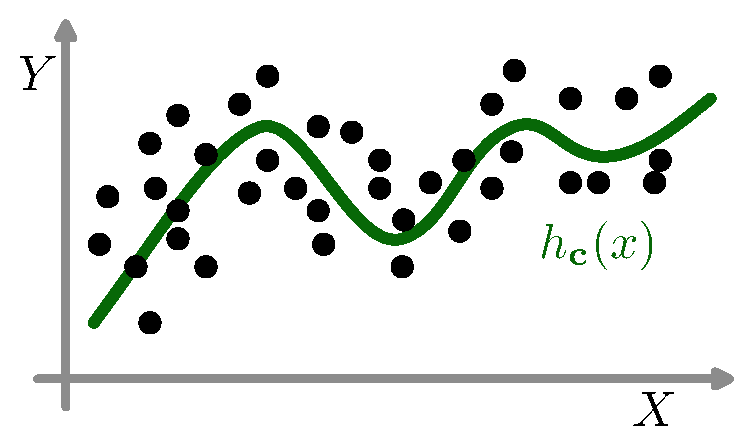
\includegraphics[width=0.45\textwidth]{chapters/notacao/regressao1.eps}
     \caption{Regressão de uma curva $h_{\VECTOR{c}}(x)$ com parâmetros $\VECTOR{c}$ num conjunto de dados. }
     \label{fig:regressao:1}
    \hspace{20pt}
\end{wrapfigure}
A regressão é o processo pelo qual uma curva ou superfície em múltiplas dimensões é 
ajustada num conjunto de dados, quando se sabe ou se aceita que existirá um erro no ajuste
devido à natureza ruidosa dos dados \cite[pp. 5]{chapra2016metodos}.

A ideia geral da regressão é achar uma curva de ajuste que represente melhor 
os dados, sem que a curva necessariamente coincida de forma exata com todos eles,
pelo que devemos definir algum critério de medida do erro de ajuste 
e procurar uma curva que minimize esse erro \cite[pp. 7]{chapra2016metodos}.

Assim, a regressão pode ser classificada mediante o tipo de curva de ajuste que é usado;
nesse sentido, podemos verificar na literatura:

\begin{itemize}
\item \textbf{Regressão linear}: 
Este caso ocorre quando usamos uma linha reta;
sendo esta uma função $h_{\VECTOR{c}}:\mathbb{R} \rightarrow \mathbb{R}$ de parâmetros $\VECTOR{c}$, 
utilizada para aproximar um conjunto de dados \cite[pp. 398, 402]{chapra2016metodos} \cite[pp. 25]{aster2013parameter}.
A regressão linear é um caso particular da regressão polinomial quando $M=1$.
\begin{example}~
\begin{itemize}
\item Curva de ajuste na regressão linear, 
\begin{equation}
h_{\VECTOR{c}}(x)=c_1+c_2 x.
\end{equation}
\item Na Seção \ref{sec:theo:reglogr1r1:1}, após uma linearização de uma relação não linear,
como na função logística, podemos ver exemplos de regressão linear.
\end{itemize}
\end{example}

\item \textbf{Regressão polinomial}: 
Indica que usamos um polinômio de grau $M$,
sendo esta uma função $h_{\VECTOR{c}}:\mathbb{R} \rightarrow \mathbb{R}$ com parâmetros $\VECTOR{c}$, 
utilizada para aproximar um conjunto de dados \cite[pp. 399, 415]{chapra2016metodos}.
\begin{example}~
\begin{itemize}
\item Curva de ajuste na regressão polinomial com grau $M=2$,
\begin{equation}
h_{\VECTOR{c}}(x)=c_1+c_2 x+c_3 x^2.
\end{equation}
\item Na Seção \ref{sec:theo:maphxr1r1}, podemos ver exemplos de regressão polinomial.
\item Na Seção \ref{sec:theo:reglogr1r1poly:1} após uma linearização de uma relação não linear,
como na função logística, podemos ver exemplos de regressão polinomial.
\end{itemize}
\end{example}

\item \textbf{Regressão não linear}: 
Neste caso, usamos um ajuste de dados
com uma função $h_{\VECTOR{c}}:\mathbb{R} \rightarrow \mathbb{R}$ com parâmetros $\VECTOR{c}$, 
que representa uma relação não linear entre o domínio e o contradomínio de $h_{\VECTOR{c}}$ 
\cite[pp. 424]{chapra2016metodos} \cite[pp. 217]{agarwal2014creators}.
\begin{example}~
\begin{itemize}
\item Um caso de curva de ajuste na regressão não linear, 
\begin{equation}
h_{\VECTOR{c}}(x)=c_1 e^{-c_2 x}.
\end{equation}
\item Na Seção \ref{sec:theo:maphcxr1r1}, podemos ver exemplos de regressão não linear.
\end{itemize}
\end{example}

\item \textbf{Regressão linear múltipla}:
Temos este caso quando ajustamos um hiperplano;
sendo esta uma função $h_{\VECTOR{c}}:\mathbb{R}^{N} \rightarrow \mathbb{R}$ com parâmetros $\VECTOR{c}$, 
utilizada para aproximar um conjunto de dados \cite[pp. 399, 418]{chapra2016metodos}.
A regressão linear é um caso particular da regressão linear múltipla quando $N=1$.
\begin{example}~
\begin{itemize}
\item Curva de ajuste na regressão linear múltipla com $N=2$, 
\begin{equation}
h_{\VECTOR{c}}(\VECTOR{x})=c_1+c_2 x_1+c_3 x_2.
\end{equation}
\item Na Seção \ref{sec:theo:reglogrnr1:1}, após uma linearização de uma relação não linear,
como na função logística, podemos ver exemplos de regressão linear múltipla.
\end{itemize}
\end{example}

\item \textbf{Regressão polinomial múltipla}:
Acontece quando ajustamos um polinômio multivariado de grau total $M$,
sendo esta uma função $h_{\VECTOR{c}}:\mathbb{R}^{N} \rightarrow \mathbb{R}$ com parâmetros $\VECTOR{c}$, 
utilizada para aproximar um conjunto de dados.
A regressão polinomial é um caso particular da regressão polinomial múltipla quando $N=1$.
\begin{example}~
\begin{itemize}
\item Um caso de curva de ajuste na regressão polinomial múltipla com 
$N=2$ e $h_{\VECTOR{c}}:\mathbb{R}^{2} \rightarrow \mathbb{R}$, 
\begin{equation}
h_{\VECTOR{c}}(\VECTOR{x})=c_1+c_2 x_1+c_3 x_2+c_4 x_1^2+c_5 x_2^2+c_6 x_1 x_2.
\end{equation}
\item Nas Seções \ref{sec:theo:maphxr2r1} e \ref{sec:theo:maphxr2r2},
 podemos ver exemplos de regressão polinomial múltipla.
\item Na Seção \ref{sec:theo:reglogrnr1poly:1}, após uma linearização de uma relação não linear,
como na função logística, podemos ver exemplos de regressão polinomial múltipla.
\end{itemize}
\end{example}

\item \textbf{Regressão não linear múltipla}: 
Estamos neste caso quado usamos no ajuste dos dados
uma função $h_{\VECTOR{c}}:\mathbb{R}^{N} \rightarrow \mathbb{R}$, 
que representa uma função não linear entre o domínio e o contradomínio de $h_{\VECTOR{c}}$.
A regressão não linear é um caso particular da regressão não linear múltipla quando $N=1$.
\begin{example}~
\begin{itemize}
\item Um caso de curva de ajuste na regressão não linear múltipla, 
\begin{equation}
h_{\VECTOR{c}}(\VECTOR{x})=c_1 e^{- c_2^2(x_1 -c_3)^2- c_4^2(x_2 -c_5)^2}.
\end{equation}
\item Na Seção \ref{sec:theo:maphcxrnr1}, podemos ver exemplos de regressão não linear múltipla.
\item Na Seção \ref{sec:theo:reglogrnr1nolinear:1}, após uma linearização de uma relação não linear,
como na função logística, podemos ver exemplos de regressão não linear múltipla.
\end{itemize}
\end{example}
\end{itemize}

\subsection{Linearização de curvas de ajuste não lineares}

Os problemas de \textbf{regressão não linear}
em alguns casos podem ser modificados para ter a forma de um 
problema de \textbf{regressão linear} (simples ou múltipla);
essa caraterística é interessante, pois geralmente
os problemas não lineares são resolvidos com métodos iterativos,
que podem ou não convergir na solução.
Em contrapartida, em problemas de regressão linear,
os métodos disponíveis nos brindam com uma resposta mediante um procedimento 
predeterminado, 
o que facilita o planejamento de um procedimento de solução e favorece o tempo de computo.

Assim, na continuação mostramos 
como problemas não lineares podem ser 
adaptados a um problema de regressão linear (simples):
\begin{example}
Usando 
$\hat{y}=ln(y)$,  
$\hat{x}=ln(x)$, 
$\hat{c}_1=ln(c_1)$, e
$\hat{c}_2=c_2$, obtemos %$\hat{y}=\hat{c}_1+\hat{c}_2 \hat{x}$.
\begin{equation}
y=c_1x^{c_2}
\quad \rightarrow \quad 
\hat{y}=\hat{c}_1+\hat{c}_2 \hat{x}.
\end{equation}
\vspace{-2pt}
\end{example}

\begin{example}%[Curva de ajuste $y=c_1 {c_2}^x$:]
Usando 
$\hat{y}=ln(y)$,  
$\hat{x}=x$, 
$\hat{c}_1=ln(c_1)$, e
$\hat{c}_2=ln(c_2)$, obtemos %$\hat{y}=\hat{c}_1+\hat{c}_2 \hat{x}$.
\begin{equation}
y=c_1 {c_2}^x
\quad \rightarrow \quad 
\hat{y}=\hat{c}_1+\hat{c}_2 \hat{x}.
\end{equation}
\vspace{-2pt}
\end{example}

\begin{example}%[Curva de ajuste $y=\left(c_1 + {c_2} x \right)^{-1}$:]
Usando 
$\hat{y}=\frac{1}{y}$,  
$\hat{x}=x$, 
$\hat{c}_1=c_1$, e 
$\hat{c}_2=c_2$, obtemos %$\hat{y}=\hat{c}_1+\hat{c}_2 \hat{x}$.
\begin{equation}
y=\left(c_1 + {c_2} x \right)^{-1}
\quad \rightarrow \quad 
\hat{y}=\hat{c}_1+\hat{c}_2 \hat{x}.
\end{equation}
\vspace{-2pt}
\end{example}

\begin{example}%[Curva de ajuste $y=c_1 x \left(c_2 + x\right)^{-1}$:] 
Usando 
$\hat{y}=\frac{1}{y}$,  
$\hat{x}=\frac{1}{x}$, 
$\hat{c}_1=\frac{1}{c_1}$, e 
$\hat{c}_2=\frac{c_2}{c_1}$, obtemos %$\hat{y}=\hat{c}_1+\hat{c}_2 \hat{x}$.
\begin{equation}
y=c_1 x \left(c_2 + x\right)^{-1}
\quad \rightarrow \quad 
\hat{y}=\hat{c}_1+\hat{c}_2 \hat{x}.
\end{equation}
\vspace{-2pt}
\end{example}

De forma similar ao caso de regressão linear simples,
curvas de ajuste não lineares podem ser adaptadas a um problema de regressão linear múltipla:
\begin{example}%[Curva de ajuste $y=c_1 +c_2 x + c_3 x^2 + c_4 x^3$:]
Usando 
$\hat{y}=y$,  
$\hat{x}_1=x$,
$\hat{x}_2=x^2$,
$\hat{x}_3=x^3$, 
$\hat{c}_1=c_1$, 
$\hat{c}_2=c_2$, 
$\hat{c}_3=c_3$, e 
$\hat{c}_4=c_4$, obtemos %$\hat{y}=\hat{c}_1+\hat{c}_2 \hat{x}_1+\hat{c}_2 \hat{x}_2+\hat{c}_3 \hat{x}_3$.
\begin{equation}
y=c_1 +c_2 x + c_3 x^2 + c_4 x^3
\quad \rightarrow \quad 
\hat{y}=\hat{c}_1+\hat{c}_2 \hat{x}_1+\hat{c}_2 \hat{x}_2+\hat{c}_3 \hat{x}_3.
\end{equation}
\vspace{-2pt}
\end{example}

\begin{example}%[Curva de ajuste $y=c_1 +c_2 \sqrt{x} + c_3 sin(x)$:]
Usando 
$\hat{y}=y$,  
$\hat{x}_1=\sqrt{x}$,
$\hat{x}_2=sin(x)$, 
$\hat{c}_1=c_1$, 
$\hat{c}_2=c_2$, e 
$\hat{c}_3=c_3$, obtemos %$\hat{y}=\hat{c}_1+\hat{c}_2 \hat{x}_1+\hat{c}_2 \hat{x}_2$.
\begin{equation}
y=c_1 +c_2 \sqrt{x} + c_3 sin(x)
\quad \rightarrow \quad 
\hat{y}=\hat{c}_1+\hat{c}_2 \hat{x}_1+\hat{c}_2 \hat{x}_2.
\end{equation}
\vspace{-2pt}
\end{example}


\newpage
%%%%%%%%%%%%%%%%%%%%%%%%%%%%%%%%%%%%%%%%%%%%%%%%%%%%%%%%%%%%%%%%%%%%%%%%%%%%%%%%
%%%%%%%%%%%%%%%%%%%%%%%%%%%%%%%%%%%%%%%%%%%%%%%%%%%%%%%%%%%%%%%%%%%%%%%%%%%%%%%%
%%%%%%%%%%%%%%%%%%%%%%%%%%%%%%%%%%%%%%%%%%%%%%%%%%%%%%%%%%%%%%%%%%%%%%%%%%%%%%%%
\section{Norma e produto interno}

A norma e o produto interno hermitiano são descritos de forma geral
na Definição \ref{def:normageral} e \ref{def:innergeral}, respetivamente.

\index{Norma em $V$!$\NORM{\VECTOR{x}}$}
\begin{definition}[Norma 
$\|\VECTOR{x}\|$ de um vetor $\VECTOR{x}$:]
\label{def:normageral}
Dado um espaço vetorial real ou complexo $V$,
a norma $\|\VECTOR{x}\|$ de um vetor $\VECTOR{x} \in V$ 
é uma função $V \rightarrow  \mathbb{R}$ 
que cumpre as seguintes três propriedades 
para todo $\VECTOR{x},\VECTOR{x}_1,\VECTOR{x}_2 \in V$ e $\alpha \in \mathbb{C}$ 
\cite[pp. 43]{d2019hermitian} \cite[pp. 27]{vetterli2014foundations}:
\begin{itemize}
\item $\|\VECTOR{x}\|> 0$ para todo vetor $\VECTOR{x}$ não nulo.
\item $\|\alpha \VECTOR{x}\|= |\alpha|~\|\VECTOR{x}\|$.
\item (Desigualdade triangular)  $\|\VECTOR{x}_1 + \VECTOR{x}_2\|< \|\VECTOR{x}_1\| + \|\VECTOR{x}_2\|$.
\end{itemize}
\end{definition}

\index{Produto interno hermitiano}
\begin{definition}[Produto interno hermitiano 
$\innerprod{\VECTOR{x}_1}{\VECTOR{x}_2}$ dos vetores $\VECTOR{x}_1$ e $\VECTOR{x}_2$:]
\label{def:innergeral}
Dado um espaço vetorial complexo $V$, 
o produto interno hermitiano $\innerprod{\VECTOR{x}_1}{\VECTOR{x}_2} $ dos vetores $\VECTOR{x}_1,\VECTOR{x}_2 \in V$ 
é uma função $V\times V \rightarrow \mathbb{C}$, 
que cumpre as seguintes quatro propriedades para todo 
$\VECTOR{x}_1,\VECTOR{x}_2,\VECTOR{x}_3 \in V$ e $\alpha \in \mathbb{C}$
 \cite[pp. 44]{d2019hermitian} \cite[pp. 242]{damiano2011course}:
\begin{itemize}
\item $\innerprod{\VECTOR{x}_1+\VECTOR{x}_2}{\VECTOR{x}_3} = \innerprod{\VECTOR{x}_1}{\VECTOR{x}_3} + \innerprod{\VECTOR{x}_2}{\VECTOR{x}_3}$.
\item Linearidade do primeiro argumento: $\innerprod{\alpha \VECTOR{x}_1}{\VECTOR{x}_2} =\alpha \innerprod{\VECTOR{x}_1}{\VECTOR{x}_2}$.
\item Simetria hermitiana: $\innerprod{\VECTOR{x}_1}{\VECTOR{x}_2} =\overline{ \innerprod{\VECTOR{x}_2}{\VECTOR{x}_1}}$.
\item Definição positiva: $\innerprod{\VECTOR{x}_1}{\VECTOR{x}_1} > 0 $  para todo $\VECTOR{x}_1$ não nulo.
\end{itemize}
\end{definition}

\begin{tcbattention}
\begin{itemize}
\item \textbf{Forma sesquilinear:} 
É importante ressaltar que dados os vetores $\VECTOR{x}_1,\VECTOR{x}_2 \in V$ 
 e $\alpha \in \mathbb{C}$ \cite[pp. 242]{damiano2011course},
\begin{equation}
\innerprod{ \VECTOR{x}_1}{\alpha \VECTOR{x}_2} =\overline{\alpha} \innerprod{\VECTOR{x}_1}{\VECTOR{x}_2}.
\end{equation}
\begin{comment}
\item \textbf{Produto interno hermitiano (real):} Dados os vetores $\VECTOR{x}_1,\VECTOR{x}_2 \in V$,
sendo $V$ um espaço vetorial real, se cumpre que
\begin{equation}
\innerprod{ \VECTOR{x}_1}{ \VECTOR{x}_2} =\innerprod{ \VECTOR{x}_2}{ \VECTOR{x}_1}.
\end{equation}
\end{comment}
\end{itemize}
\end{tcbattention}

\begin{definition}[Produto interno hermitiano vs. norma euclidiana quadrada:]
Dado um vetor $\VECTOR{x}$ dentro de um espaço vetorial real ou complexo $V$,
podemos estabelecer a seguinte relação entre o 
produto interno hermitiano $\innerprod{\VECTOR{x}}{\VECTOR{x}}$ e 
a norma euclidiana quadrada $\|\VECTOR{x}\|$ 
\cite[pp. 44]{d2019hermitian}  \cite[pp. 242]{damiano2011course}
\begin{equation}
\|\VECTOR{x}\|=\sqrt{\innerprod{\VECTOR{x}}{\VECTOR{x}}},
\end{equation} 
\end{definition}

\begin{tcbattention}
\begin{itemize}
\item Um produto interno hermitiano pode ser usado para representar uma norma,
porém não todas as normas podem ser representas por um produto interno 
(ver Seção \ref{subsec:pnorm}) \cite[pp. 45]{d2019hermitian}.
\end{itemize}
\end{tcbattention}

Dessas descrições gerais podem ser definidos diversos casos para as funções
norma e o produto interno hermitiano; assim, 
nas seguintes subseções, serão mostrados alguns desses casos.

%%%%%%%%%%%%%%%%%%%%%%%%%%%%%%%%%%%%%%%%%%%%%%%%%%%%%%%%%%%%%%%%%%%%%%%%%%%%%%%%
\subsection{Produto interno hermitiano em $\mathbb{C}^N$}

\index{Produto interno hermitiano!Canônico $\innerprod{\VECTOR{x}_1}{\VECTOR{x}_2}$}
\begin{definition}[Produto interno hermitiano (canônico)
em $\mathbb{C}^N$:]
Dado, $\mathbb{C}^N$, um espaço euclideano complexo de dimensão $N$;
o produto interno hermitiano $\innerprod{\VECTOR{u}}{\VECTOR{v}}$ dos vetores $\VECTOR{u},\VECTOR{v} \in \mathbb{C}^N$
é definido como \cite[pp. 44]{d2019hermitian} \cite[pp. 242]{damiano2011course}
\begin{equation}
\innerprod{\VECTOR{u}}{\VECTOR{v}}=\VECTOR{u}^{\transpose} \overline{\VECTOR{v}}=\sum_{n=1}^N u_n \overline{v_n},
\end{equation} 
em que $\VECTOR{u}=[u_1,~u_2,~...,~u_n,~...,~u_N]^{\transpose}$ e $\VECTOR{v}=[v_1,~v_2,~...,~v_n,~...,~v_N]^{\transpose}$.
\end{definition}

\index{Produto interno hermitiano!Genérico $\innerprod{\VECTOR{x}_1}{\VECTOR{x}_2}_{\MATRIX{A}}$}
\begin{definition}[Produto interno hermitiano genérico
em $\mathbb{C}^N$:]
Dado, $\mathbb{C}^N$, um espaço euclideano complexo de dimensão $N$ e
$\MATRIX{A}$ uma \hyperref[def:hermitianapositivamatrix0]{\textbf{matriz hermitiana definida positiva}};
o produto interno hermitiano genérico $\innerprod{\VECTOR{u}}{\VECTOR{v}}_{\MATRIX{A}}$ 
dos vetores $\VECTOR{u},\VECTOR{v} \in \mathbb{C}^N$ 
%com $\VECTOR{u}=[u_1,~u_2,~...,~u_n,~...,~u_N]$ e $\VECTOR{v}=[v_1,~v_2,~...,~v_n,~...,~v_N]$,
é definido como \cite[pp. 1358]{weisstein2002crc}:
\begin{equation}
\innerprod{\VECTOR{u}}{\VECTOR{v}}_{\MATRIX{A}}=\VECTOR{u}^{\transpose} \MATRIX{A} \overline{\VECTOR{v}}.
\end{equation} 
\end{definition}

%%%%%%%%%%%%%%%%%%%%%%%%%%%%%%%%%%%%%%%%%%%%%%%%%%%%%%%%%%%%%%%%%%%%%%%%%%%%%%%%
\subsection{Norma em $\mathbb{C}^N$}

\index{Norma em $\mathbb{C}^N$!$\NORM{\VECTOR{x}}$}
\begin{definition}[Norma (canônica)
em $\mathbb{C}^N$:]
Dado, $\mathbb{C}^N$, um espaço euclideano complexo de dimensão $N$;
a norma  $\|\VECTOR{x}\|$ do vetor $\VECTOR{x}\in \mathbb{C}^N$
%com $\VECTOR{x}=[x_1,~x_2,~...,~x_n,~...,~x_N]^{\transpose}$,
é definida como:
\begin{equation}
\|\VECTOR{x}\|=\sqrt{\innerprod{\VECTOR{x}}{\VECTOR{x}}}
=\sqrt{\VECTOR{x}^{\transpose} \overline{\VECTOR{x}}}
%=\sqrt{\sum_{n=1}^N x_n \overline{x_n}}
,
\end{equation} 
\begin{equation}
\|\VECTOR{x}\|^2=\innerprod{\VECTOR{x}}{\VECTOR{x}}
=\VECTOR{x}^{\transpose} \overline{\VECTOR{x}}
%=\sum_{n=1}^N x_n \overline{x_n}
.
\end{equation} 
\end{definition}

\index{Norma em $\mathbb{C}^N$!$\NORM{\VECTOR{x}}_{\MATRIX{A}}$}
\begin{definition}[Norma genérica
em $\mathbb{C}^N$:]
Dado $\mathbb{C}^N$, um espaço euclideano complexo de dimensão $N$;
a norma  $\|\VECTOR{x}\|_{\MATRIX{A}}$ do vetor $\VECTOR{x}\in \mathbb{C}^N$
ponderada com a matriz $\MATRIX{A}$ \hyperref[def:hermitianapositivematrix0]{\textbf{hermitiana definida positiva}},
%com $\VECTOR{x}=[x_1,~x_2,~...,~x_n,~...,~x_N]^{\transpose}$,
é definido como:
\vspace{-10pt}
\begin{equation}
\|\VECTOR{x}\|_{\MATRIX{A}}=\sqrt{\innerprod{\VECTOR{x}}{\VECTOR{x}}_{\MATRIX{A}}}
=\sqrt{\VECTOR{x}^{\transpose}\MATRIX{A} \overline{\VECTOR{x}}}
%=\sqrt{\sum_{i,j=1}^N a_{ij}x_i \overline{x_j}}
,
\end{equation} 
\begin{equation}
\|\VECTOR{x}\|_{\MATRIX{A}}^2=\innerprod{\VECTOR{x}}{\VECTOR{x}}_{\MATRIX{A}}
=\VECTOR{x}^{\transpose}\MATRIX{A} \overline{\VECTOR{x}}
%=\sum_{i,j=1}^N a_{ij}x_i \overline{x_j}
.
\end{equation} 
\end{definition}

\begin{tcbattention}
\begin{itemize}
\item Quando $\MATRIX{A}=\funcdiag\left([a_1,~a_2,~...,~a_N]^{\transpose}\right)$ 
é uma matriz real e diagonal e
$\VECTOR{x}=[x_1,~x_2,~...,~x_N]^{\transpose} \in \mathbb{C}^N$, 
a norma quadrada genérica $\|\VECTOR{x}\|_{\MATRIX{A}}^2$ é igual a
\vspace{-10pt}
\begin{equation}
\|\VECTOR{x}\|_{\MATRIX{A}}^2=\sum_{n=1}^{N} a_{n}|x_n|^2
\end{equation}
\end{itemize}
\end{tcbattention}

%%%%%%%%%%%%%%%%%%%%%%%%%%%%%%%%%%%%%%%%%%%%%%%%%%%%%%%%%%%%%%%%%%%%%%%%%%%%%%%%
%\subsection{Norma}
\index{Norma em $\mathbb{C}^N$!$\NORM{\VECTOR{x}}_{p}$}
\subsection{Norma $p$ em dimensões finitas} %standard normed vector spaces
\label{subsec:pnorm}
\begin{wrapfigure}{r}{0.5\textwidth}
     \centering
     \vspace{-15pt}
     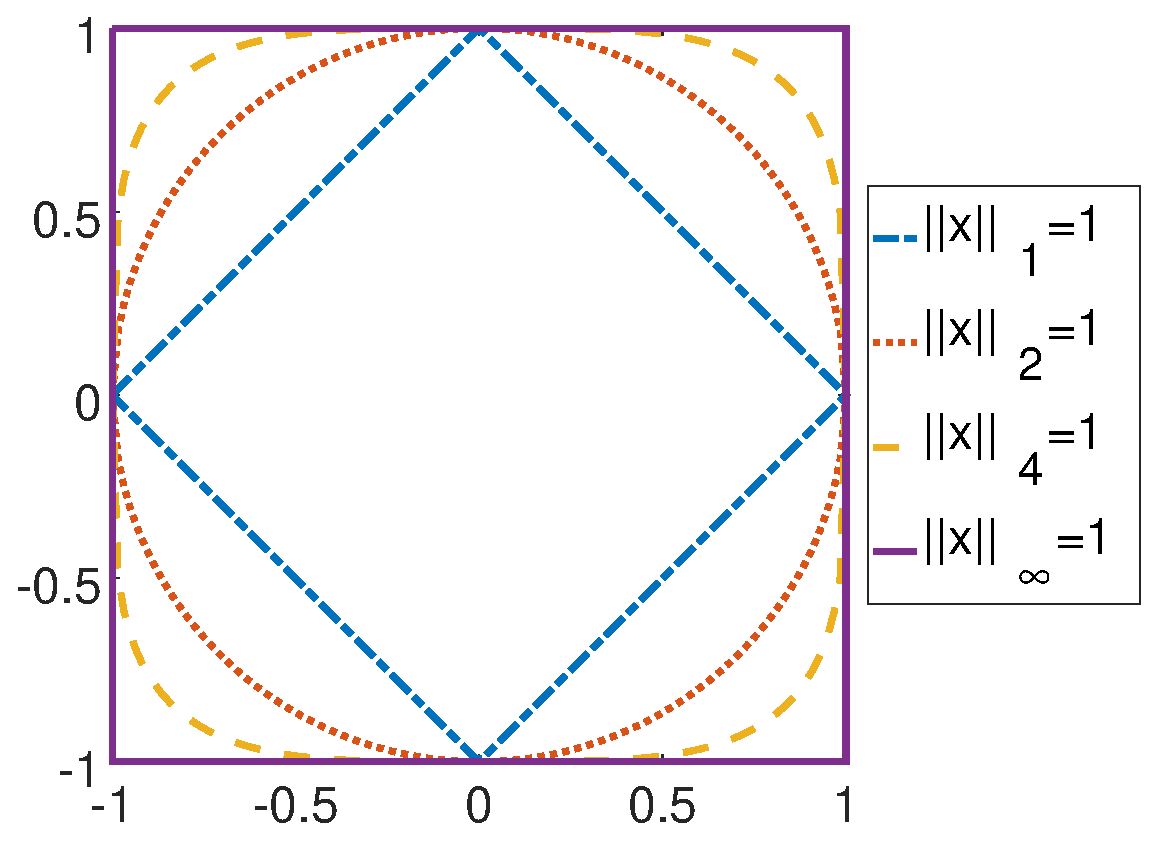
\includegraphics[width=0.45\textwidth]{chapters/notacao/pnormcode.eps}
     \caption{Curva de norma unitária.}
     \label{fig:curvaunit}
     \vspace{-30pt}
\end{wrapfigure}
Dado um vetor $\VECTOR{x} \in \mathbb{C}^{N}$,
é definida a norma $p$ de $\VECTOR{x}$  como $\|\VECTOR{x}\|_p$ \cite[pp. 33]{vetterli2014foundations}, 
\begin{equation}
\|\VECTOR{x}\|_p=\left(\sum_{n=1}^N |x_n|^p\right)^{\frac{1}{p}},
\end{equation}
em que $1 \leq p < \infty$; a norma $p$
também é denotada como norma $L_p$ ou ``$p$-norm'' em inglês.
Assim, dependendo do valor de $p$, entraremos em vários casos ou tipos de norma,
a Fig. \ref{fig:curvaunit} e os seguintes exemplos mostram alguns desses tipos.

\begin{example}[Norma taxicab - $p=1$:] Também chamada norma Manhattan
\begin{equation}
\|\VECTOR{x}\|_1=\sum_{n=1}^N |x_n|.
\end{equation}
\end{example}

\begin{example}[Norma euclidiana - $p=2$:] Também chamada norma euclidiana quadrada, 
a qual também pode ser representada como $\|\VECTOR{x}\|$; 
assim, ante a ausência de subíndice se entende que é a $2$-norm,
\begin{equation}
\|\VECTOR{x}\|_2\equiv \|\VECTOR{x}\| =\sqrt{\sum_{n=1}^N |x_n|^2}.
\end{equation}
Uma representação relativa à norma quadrada euclidiana é
\begin{equation}
\|\VECTOR{x}\|_2^2\equiv \|\VECTOR{x}\|^2=\sum_{n=1}^N |x_n|^2\equiv \VECTOR{x}^{*} \VECTOR{x},
\end{equation}
em que $\VECTOR{x}^{*}\equiv \VECTOR{\bar{x}}^{\transpose}$ 
representa a transposta do conjugado do vetor  $\VECTOR{x}$. 
\end{example}

\begin{example}[Norma com $p=\infty$:]
\begin{equation}
\|\VECTOR{x}\|_{\infty}=\max \left( |x_1|,~|x_2|,~...,~|x_n|,~...,~|x_N|\right)\equiv \max_n \left( |x_n|\right).
\end{equation}
\end{example}




%----------------------------------------------------------------------------------------
%	CHAPTER  
%----------------------------------------------------------------------------------------
\chapterimage{chapter_function.pdf} % Chapter heading image

\chapter{Funções e operadores notáveis}

%%%%%%%%%%%%%%%%%%%%%%%%%%%%%%%%%%%%%%%%%%%%%%%%%%%%%%%%%%%%%%%%%%%%%%%%%%%%%%%%
%\newpage
%%%%%%%%%%%%%%%%%%%%%%%%%%%%%%%%%%%%%%%%%%%%%%%%%%%%%%%%%%%%%%%%%%%%%%%%%%%%%%%%%%%%%%%
%%%%%%%%%%%%%%%%%%%%%%%%%%%%%%%%%%%%%%%%%%%%%%%%%%%%%%%%%%%%%%%%%%%%%%%%%%%%%%%%%%%%%%%
%%%%%%%%%%%%%%%%%%%%%%%%%%%%%%%%%%%%%%%%%%%%%%%%%%%%%%%%%%%%%%%%%%%%%%%%%%%%%%%%%%%%%%%
\section{Mnemônico vetor nabla $\vec{\triangledown}$}

\begin{notation}[Uso do Mnemônico vetor nabla 
($\overrightarrow{\triangledown}$ ):]
Dado um vetor coluna $\VECTOR{x}\in \mathbb{R}^N$, usaremos o mnemônico\footnote{Falando de um modo rigoroso, 
 $\overrightarrow{\triangledown}$ não é um operador diferencial, 
e sim um mnemônico que nos ajuda a lembrar e representar uma série de operadores diferenciais.} 
vetor nabla ($\overrightarrow{\triangledown}$), como:
\begin{equation}
\overrightarrow{\triangledown}  \equiv \frac{\partial }{\partial \VECTOR{x}} =
\begin{bmatrix}
\frac{\partial  }{\partial x_{1}}\\
\frac{\partial  }{\partial x_{2}}\\
\vdots\\
\frac{\partial  }{\partial x_{n}}\\
\vdots\\
\frac{\partial  }{\partial x_{N}}
\end{bmatrix}
\end{equation}
\end{notation}
~

\begin{tcbattention}
Não deve ser confundido o mnemônico $\overrightarrow{\triangledown}$, 
com o operador $\triangledown$, cujo uso será explicado nas seguintes seções.
\end{tcbattention}
~

\begin{definition}[Derivada 
$\overrightarrow{\triangledown}^{\transpose}\VECTOR{f}(\VECTOR{x})$:]
\label{def:nabla:dot}
Dado 
um vetor coluna $\VECTOR{x}\in \mathbb{R}^N$ e 
uma função vetor coluna $\VECTOR{f}(\VECTOR{x}): \mathbb{R}^N \rightarrow \mathbb{R}^M$, 
definimos que:
\begin{equation}
\overrightarrow{\triangledown}.~\VECTOR{f}(\VECTOR{x}) \equiv
\overrightarrow{\triangledown}^{\transpose}\VECTOR{f}(\VECTOR{x})= 
\frac{\partial f_{1}(\VECTOR{x}) }{\partial x_{1}}+
\frac{\partial f_{2}(\VECTOR{x}) }{\partial x_{2}}+
\hdots+
\frac{\partial f_{n}(\VECTOR{x}) }{\partial x_{n}}+
\hdots+
\frac{\partial f_{N}(\VECTOR{x}) }{\partial x_{N}}=
\sum \limits_{n=1}^N \frac{\partial f_{n}(\VECTOR{x}) }{\partial x_{n}}
\end{equation}

\end{definition}


%%%%%%%%%%%%%%%%%%%%%%%%%%%%%%%%%%%%%%%%%%%%%%%%%%%%%%%%%%%%%%%%%%%%%%%%%%%%%%%%
\newpage

%%%%%%%%%%%%%%%%%%%%%%%%%%%%%%%%%%%%%%%%%%%%%%%%%%%%%%%%%%%%%%%%%%%%%%%%%%%%%%%%%%%%%%%
%%%%%%%%%%%%%%%%%%%%%%%%%%%%%%%%%%%%%%%%%%%%%%%%%%%%%%%%%%%%%%%%%%%%%%%%%%%%%%%%%%%%%%%
%%%%%%%%%%%%%%%%%%%%%%%%%%%%%%%%%%%%%%%%%%%%%%%%%%%%%%%%%%%%%%%%%%%%%%%%%%%%%%%%%%%%%%%
\section{Operador derivada para $e(\VECTOR{x})$, $\VECTOR{f}(\VECTOR{x})$ e  $\MATRIX{G}(\VECTOR{x})$}

%%%%%%%%%%%%%%%%%%%%%%%%%%%%%%%%%%%%%%%%%%%%%%%%%%%%%%%%%%%%%%%%%%%%%%%%%%%%%%%%
\subsection{Derivadas a respeito de $\VECTOR{x}^{\transpose}$}

\begin{definition}[Derivada de 
$e(\VECTOR{x})$ a respeito de $\VECTOR{x}^{\transpose}$:]\label{def:deltahor}
Dado 
um vetor coluna $\VECTOR{x}\in \mathbb{R}^N$ e 
uma função $e(\VECTOR{x}): \mathbb{R}^N \rightarrow \mathbb{R}$,
definimos que:
\begin{equation}
\left[\overrightarrow{\triangledown} e(\VECTOR{x})\right]^{\transpose} \equiv 
\frac{\partial e(\VECTOR{x}) }{\partial \VECTOR{x}^{\transpose}}= 
\left[
\begin{matrix}
\frac{\partial e(\VECTOR{x}) }{\partial x_{1}}&
\frac{\partial e(\VECTOR{x}) }{\partial x_{2}}&
\hdots&
\frac{\partial e(\VECTOR{x}) }{\partial x_{n}}&
\hdots&
\frac{\partial e(\VECTOR{x}) }{\partial x_{N}}
\end{matrix}
\right]= {\bigcup\limits_{n=1}^{\rightarrow}}^{N}{\frac{\partial e(\VECTOR{x}) }{\partial x_{n}}} 
\end{equation}
\end{definition}

\begin{definition}[Derivada de 
$\VECTOR{f}(\VECTOR{x})$ a respeito de $\VECTOR{x}^{\transpose}$:]\label{def:deltahor2}
Dado 
um vetor coluna $\VECTOR{x}\in \mathbb{R}^N$ e 
uma função vetor coluna $\VECTOR{f}(\VECTOR{x}): \mathbb{R}^N \rightarrow \mathbb{R}^M$, 
definimos que:
\begin{equation}
\left[\overrightarrow{\triangledown} \VECTOR{f}^{\transpose}(\VECTOR{x})\right]^{\transpose} \equiv 
\frac{\partial \VECTOR{f}(\VECTOR{x}) }{\partial \VECTOR{x}^{\transpose}}= 
\left[
\begin{matrix}
\frac{\partial \VECTOR{f}(\VECTOR{x}) }{\partial x_{1}}&
\frac{\partial \VECTOR{f}(\VECTOR{x}) }{\partial x_{2}}&
\hdots&
\frac{\partial \VECTOR{f}(\VECTOR{x}) }{\partial x_{n}}&
\hdots&
\frac{\partial \VECTOR{f}(\VECTOR{x}) }{\partial x_{N}}
\end{matrix}
\right]= {\bigcup\limits_{n=1}^{\rightarrow}}^{N}{\frac{\partial \VECTOR{f}(\VECTOR{x}) }{\partial x_{n}}} 
\end{equation}
\end{definition}

\begin{definition}[Derivada de 
$\MATRIX{G}(\VECTOR{x})$ a respeito de $\VECTOR{x}^{\transpose}$:]\label{def:deltahor3}
Dado 
um vetor coluna $\VECTOR{x}\in \mathbb{R}^N$ e 
uma função $\MATRIX{G}(\VECTOR{x}): \mathbb{R}^N \rightarrow \mathbb{R}^{M\times L}$, 
definimos que:
\begin{equation}
\frac{\partial \MATRIX{G}(\VECTOR{x}) }{\partial \VECTOR{x}^{\transpose}}= 
\left[
\begin{matrix}
\frac{\partial \MATRIX{G}(\VECTOR{x}) }{\partial x_{1}}&
\frac{\partial \MATRIX{G}(\VECTOR{x}) }{\partial x_{2}}&
\hdots&
\frac{\partial \MATRIX{G}(\VECTOR{x}) }{\partial x_{n}}&
\hdots&
\frac{\partial \MATRIX{G}(\VECTOR{x}) }{\partial x_{N}}
\end{matrix}
\right]= {\bigcup\limits_{n=1}^{\rightarrow}}^{N}{\frac{\partial \MATRIX{G}(\VECTOR{x}) }{\partial x_{n}}}.
\end{equation}
\end{definition}

\begin{comment}
Assim, obtemos o vetor linha
$\frac{\partial e(\VECTOR{x}) }{\partial \VECTOR{x}^{\transpose}} \in \mathbb{R}^{1\times N}$,
as matrizes
$\frac{\partial \VECTOR{f}(\VECTOR{x}) }{\partial \VECTOR{x}^{\transpose}} \in \mathbb{R}^{M \times N}$ e
$\frac{\partial \VECTOR{g}(\VECTOR{x}) }{\partial \VECTOR{x}^{\transpose}} \in \mathbb{R}^{M \times (LN)}$.
\end{comment}

\begin{example}[Uso da Definição \ref{def:deltahor}:]
Conhecida a função $e(\VECTOR{x}): \mathbb{R}^2 \rightarrow \mathbb{R}$, podemos calcular,
\begin{equation}
e(\VECTOR{x})=x_1^2+x_1 x_2+x_2^2
\qquad \rightarrow \qquad
\frac{\partial e(\VECTOR{x}) }{\partial \VECTOR{x}^{\transpose}}=
\left[ 2 x_1+x_2 \quad x_1 + 2 x_2\right]
\end{equation}
\end{example}


\begin{example}[Uso da Definição \ref{def:deltahor2}:]
Conhecida a função $\VECTOR{f}(\VECTOR{x}): \mathbb{R}^2 \rightarrow \mathbb{R}^4$, podemos calcular,
\begin{equation}
\VECTOR{f}(\VECTOR{x})=
\begin{bmatrix}
x_1^2+x_2\\
x_1+x_2^2\\
x_1 x_2 \\
x_1^2+x_2^2
\end{bmatrix}
\qquad \rightarrow \qquad
\frac{\partial \VECTOR{f}(\VECTOR{x}) }{\partial \VECTOR{x}^{\transpose}}= 
\begin{bmatrix}
2 x_1 & 1\\
1     & 2 x_2\\
x_2   & x_1\\
2 x_1 & 2 x_2
\end{bmatrix}
\end{equation}
\end{example}

\begin{example}[Uso da Definição \ref{def:deltahor3}:]
Conhecida a função $\MATRIX{G}(\VECTOR{x}): \mathbb{R}^2 \rightarrow \mathbb{R}^{3 \times 2}$, podemos calcular,
\begin{equation}
\MATRIX{G}(\VECTOR{x})=
\begin{bmatrix}
x_1^2       & x_1 x_2\\
x_1 x_2     & x_2^2\\
x_1^2 + x_2 & x_1 + x_2^2\\
x_1 + x_2   & x_1 + x_2
\end{bmatrix}
\qquad \rightarrow \qquad
\frac{\partial \MATRIX{G}(\VECTOR{x}) }{\partial \VECTOR{x}^{\transpose}}= 
\begin{bmatrix}
2 x_1 & x_2 & 0   &   x_1\\
  x_2 & 0   & x_1 & 2 x_2\\
2 x_1 & 1   & 1   & 2 x_2\\
    1 & 1   & 1   & 1
\end{bmatrix}
\end{equation}
\end{example}
%%%%%%%%%%%%%%%%%%%%%%%%%%%%%%%%%%%%%%%%%%%%%%%%%%%%%%%%%%%%%%%%%%%%%%%%%%%%%%%%
\subsection{Derivadas a respeito de $\VECTOR{x}$}

\begin{definition}[Derivada de 
$e(\VECTOR{x})$ a respeito de $\VECTOR{x}$:]\label{def:deltaver}
Dado 
um vetor coluna $\VECTOR{x}\in \mathbb{R}^N$ e 
uma função $e(\VECTOR{x}): \mathbb{R}^N \rightarrow \mathbb{R}$,
definimos que:
\begin{equation}
\overrightarrow{\triangledown} e(\VECTOR{x}) \equiv 
\frac{\partial e(\VECTOR{x}) }{\partial \VECTOR{x}}= 
\left[
\begin{matrix}
\frac{\partial e(\VECTOR{x}) }{\partial x_{1}} \\
\frac{\partial e(\VECTOR{x}) }{\partial x_{2}} \\
\vdots \\
\frac{\partial e(\VECTOR{x}) }{\partial x_{n}} \\
\vdots \\
\frac{\partial e(\VECTOR{x}) }{\partial x_{N-1}} \\
\frac{\partial e(\VECTOR{x}) }{\partial x_{N}} 
\end{matrix}
\right] = 
{\bigcup\limits_{n=1}^{\downarrow}}^{N}{\frac{\partial e(\VECTOR{x}) }{\partial x_{n}}} 
\end{equation}
\end{definition}

\begin{definition}[Derivada de 
$\VECTOR{f}(\VECTOR{x})$ a respeito de $\VECTOR{x}$:]\label{def:deltaver2}
Dado 
um vetor coluna $\VECTOR{x}\in \mathbb{R}^N$ e 
uma função vetor coluna $\VECTOR{f}(\VECTOR{x}): \mathbb{R}^N \rightarrow \mathbb{R}^M$, 
definimos que:
\begin{equation}
\frac{\partial \VECTOR{f}(\VECTOR{x}) }{\partial \VECTOR{x}}= 
\left[
\begin{matrix}
\frac{\partial \VECTOR{f}(\VECTOR{x}) }{\partial x_{1}} \\
\frac{\partial \VECTOR{f}(\VECTOR{x}) }{\partial x_{2}} \\
\vdots \\
\frac{\partial \VECTOR{f}(\VECTOR{x}) }{\partial x_{n}} \\
\vdots \\
%\frac{\partial \VECTOR{f}(\VECTOR{x}) }{\partial x_{N-1}} \\
\frac{\partial \VECTOR{f}(\VECTOR{x}) }{\partial x_{N}}
\end{matrix}
\right] =  
{\bigcup\limits_{n=1}^{\downarrow}}^{N}{\frac{\partial \VECTOR{f}(\VECTOR{x}) }{\partial x_{n}}}
\end{equation}
\end{definition}

\begin{definition}[Derivada de 
$\MATRIX{G}(\VECTOR{x})$ a respeito de $\VECTOR{x}$:]\label{def:deltaver3}
Dado 
um vetor coluna $\VECTOR{x}\in \mathbb{R}^N$ e 
uma função $\MATRIX{G}(\VECTOR{x}): \mathbb{R}^N \rightarrow \mathbb{R}^{M\times L}$, 
definimos que:
\begin{equation}
\frac{\partial \MATRIX{G}(\VECTOR{x}) }{\partial \VECTOR{x}}= 
\left[
\begin{matrix}
\frac{\partial \MATRIX{G}(\VECTOR{x}) }{\partial x_{1}} \\
\frac{\partial \MATRIX{G}(\VECTOR{x}) }{\partial x_{2}} \\
\vdots \\
\frac{\partial \MATRIX{G}(\VECTOR{x}) }{\partial x_{n}} \\
\vdots \\
%\frac{\partial \MATRIX{G}(\VECTOR{x}) }{\partial x_{N-1}} \\
\frac{\partial \MATRIX{G}(\VECTOR{x}) }{\partial x_{N}}
\end{matrix}
\right] = {\bigcup\limits_{n=1}^{\downarrow}}^{N}{\frac{\partial \MATRIX{G}(\VECTOR{x}) }{\partial x_{n}}}
\end{equation}
\end{definition}

\begin{comment}
Assim, 
$\frac{\partial e(\VECTOR{x}) }{\partial \VECTOR{x}} \in \mathbb{R}^{N \times 1}$,
$\frac{\partial \VECTOR{f}(\VECTOR{x}) }{\partial \VECTOR{x}} \in \mathbb{R}^{(MN) \times 1}$ e
$\frac{\partial \VECTOR{g}(\VECTOR{x}) }{\partial \VECTOR{x}} \in \mathbb{R}^{(MN) \times L}$.
\end{comment}


\begin{corollary}[Igualdade das derivadas cruzadas]\label{cor:derder}
Dado,
o vetor coluna $\VECTOR{x}\in \mathbb{R}^N$, 
a função $e(\VECTOR{x}): \mathbb{R}^N \rightarrow \mathbb{R}$; e
considerando as Definições \ref{def:deltahor}, \ref {def:deltaver} e o 
teorema da igualdade das derivadas cruzadas\footnote{Tambem conhecido como 
``teorema de Clairaut'' \cite[pp. 885]{stewart2008calculus},
 ``teorema de Clairaut-Schwarz'' \cite[pp. 311]{telles2015matematica}, ou ``teorema de Schwarz''.}; 
podemos deduzir que:
\begin{equation}
 \frac{\partial }{\partial \VECTOR{x}} \left( \frac{\partial e(\VECTOR{x} )}{\partial \VECTOR{x}^{\transpose}} \right) = 
\frac{\partial }{\partial \VECTOR{x}^{\transpose}} \left( \frac{\partial e(\VECTOR{x} )}{\partial \VECTOR{x}} \right)
\end{equation}
\end{corollary}

%%%%%%%%%%%%%%%%%%%%%%%%%%%%%%%%%%%%%%%%%%%%%%%%%%%%%%%%%%%%%%%%%%%%%%%%%%%%%%%%

\begin{example}[Uso da Definição \ref{def:deltaver}:]
Conhecida a função $e(\VECTOR{x}): \mathbb{R}^2 \rightarrow \mathbb{R}$, podemos calcular,
\begin{equation}
e(\VECTOR{x})=x_1^2+x_1 x_2+x_2^2
\qquad \rightarrow \qquad
\frac{\partial e(\VECTOR{x}) }{\partial \VECTOR{x}}=
\begin{bmatrix}
 2 x_1 + x_2 \\
 x_1 + 2 x_2
\end{bmatrix}
\end{equation}
\end{example}


\begin{example}[Uso da Definição \ref{def:deltaver2}:]
Conhecida a função $\VECTOR{f}(\VECTOR{x}): \mathbb{R}^2 \rightarrow \mathbb{R}^4$, podemos calcular,
\begin{equation}
\VECTOR{f}(\VECTOR{x})=
\begin{bmatrix}
x_1^2+x_2\\
x_1+x_2^2\\
x_1 x_2 \\
x_1^2+x_2^2
\end{bmatrix}
\qquad \rightarrow \qquad
\frac{\partial \VECTOR{f}(\VECTOR{x}) }{\partial \VECTOR{x}}= 
\begin{bmatrix}
2 x_1 \\
1     \\
x_2   \\
2 x_1 \\
1     \\
2 x_2 \\
x_1   \\
2 x_2
\end{bmatrix}
\end{equation}
\end{example}


\begin{example}[Uso da Definição \ref{def:deltaver3}:]
Conhecida a função $\MATRIX{G}(\VECTOR{x}): \mathbb{R}^2 \rightarrow \mathbb{R}^{3 \times 2}$, podemos calcular,
\begin{equation}
\MATRIX{G}(\VECTOR{x})=
\begin{bmatrix}
x_1^2       & x_1 x_2\\
x_1 x_2     & x_2^2\\
x_1^2 + x_2 & x_1 + x_2^2\\
x_1 + x_2   & x_1 + x_2
\end{bmatrix}
\qquad \rightarrow \qquad
\frac{\partial \MATRIX{G}(\VECTOR{x}) }{\partial \VECTOR{x}}= 
\begin{bmatrix}
2 x_1 & x_2\\ 
  x_2 & 0  \\ 
2 x_1 & 1  \\ 
    1 & 1  \\ 
0   &   x_1\\
x_1 & 2 x_2\\
1   & 2 x_2\\
1   & 1
\end{bmatrix}
\end{equation}
\end{example}

\begin{example}[Uso do Corolário \ref{cor:derder}:]
Conhecida a função $e(\VECTOR{x}): \mathbb{R}^2 \rightarrow \mathbb{R}$, podemos calcular,
\begin{equation}
e(\VECTOR{x})=x_1^2+x_1 x_2+x_2^2
\qquad \rightarrow \qquad
\frac{\partial^2 e(\VECTOR{x}) }{\partial \VECTOR{x} \partial \VECTOR{x}^{\transpose}}=
\frac{\partial^2 e(\VECTOR{x}) }{\partial \VECTOR{x}^{\transpose} \partial \VECTOR{x}}=
\begin{bmatrix}
 2 & 1 \\
 1 & 2
\end{bmatrix}
\end{equation}
\end{example}

\index{Schwarz, Karl Hermann Amandus}
\begin{elaboracion}[title=Karl Hermann Amandus Schwarz (1843-1921), width= 0.99\linewidth]
Matemático nascido em Jerzmanowa (Polônia), porém  educado na Alemanha.
Foi membro da Academia de Ciências de Berlim e professor da Universidade de Berlim,
Ele é lembrado pelo método aditivo de Schwarz,lema de Schwarz, o mapeamento de Schwarz-Christoffel, 
o teorema de Schwarz (teorema da igualdade das derivadas cruzadas), o teorema Schwarz-Ahlfors-Pick, entre outros \cite[pp. 297]{agarwal2014creators}.
\end{elaboracion}



%%%%%%%%%%%%%%%%%%%%%%%%%%%%%%%%%%%%%%%%%%%%%%%%%%%%%%%%%%%%%%%%%%%%%%%%%%%%%%%%
\newpage

%%%%%%%%%%%%%%%%%%%%%%%%%%%%%%%%%%%%%%%%%%%%%%%%%%%%%%%%%%%%%%%%%%%%%%%%%%%%%%%%%%%%%%%
%%%%%%%%%%%%%%%%%%%%%%%%%%%%%%%%%%%%%%%%%%%%%%%%%%%%%%%%%%%%%%%%%%%%%%%%%%%%%%%%%%%%%%%
%%%%%%%%%%%%%%%%%%%%%%%%%%%%%%%%%%%%%%%%%%%%%%%%%%%%%%%%%%%%%%%%%%%%%%%%%%%%%%%%%%%%%%%
\section{Derivadas notáveis: Gradiente, Matriz Hessiana, Matriz Jacobiana}

\begin{proposition}[$\triangledown e(\VECTOR{x})$ - Gradiente de $e(\VECTOR{x})$:]\label{def:gradient}
 Dada uma função $e:\mathbb{R}^{N}\rightarrow \mathbb{R}$ com variável $\VECTOR{x} \in \mathbb{R}^{N}$
 como vetor coluna com elementos $x_n\in \mathbb{R}$ de modo que $n\in \mathbb{N}$, $1 \leq n \leq N$,
 diferenciável em $\VECTOR{x}$. 
 $\triangledown e(\VECTOR{x})$ é chamado gradiente 
\cite[pp. 913]{stewart2008calculus} \cite[pp. 80]{telles2015matematica} \cite{Gradient}  de $e(\VECTOR{x})$, de modo que: 
\begin{equation}
\frac{\partial e(\VECTOR{x})}{\partial \VECTOR{x} }=
\left[
\begin{matrix}
\frac{\partial e(\VECTOR{x}) }{\partial x_{1}}&
\frac{\partial e(\VECTOR{x}) }{\partial x_{2}}&
\hdots&
\frac{\partial e(\VECTOR{x}) }{\partial x_{n}}&
\hdots&
\frac{\partial e(\VECTOR{x}) }{\partial x_{N}}
\end{matrix}
\right]^{\transpose}
 \end{equation}
\begin{equation}
\overrightarrow{\triangledown} e(\VECTOR{x})\equiv  
\triangledown e(\VECTOR{x}) \equiv 
\frac{\partial e(\VECTOR{x})}{\partial \VECTOR{x} }
\end{equation}
\end{proposition}
\index{Gradiente}

\noindent
\begin{minipage}{0.5\textwidth}
\begin{example}[Uso da Proposição \ref{def:gradient}:]
Conhecida a função $e(\VECTOR{x}): \mathbb{R}^2 \rightarrow \mathbb{R}$, 
\begin{equation}
e(\VECTOR{x})=x_1 e^{-x_1^2 - x_2^2},
\end{equation}
podemos calcular,
\begin{equation}
\frac{\partial e(\VECTOR{x}) }{\partial \VECTOR{x}}=
\begin{bmatrix}
(1-2 x_1^2) e^{-x_1^2 - x_2^2}\\
-2 x_1 x_2 e^{-x_1^2 - x_2^2}
\end{bmatrix}
\end{equation}
Um gráfico de $\frac{\partial e(\VECTOR{x}) }{\partial \VECTOR{x}}$ pode ser visto na Figura \ref{fig:ex:gradient}.
\end{example}
\end{minipage}
\begin{minipage}{0.45\textwidth}
    \begin{figure}[H]
	\centering
        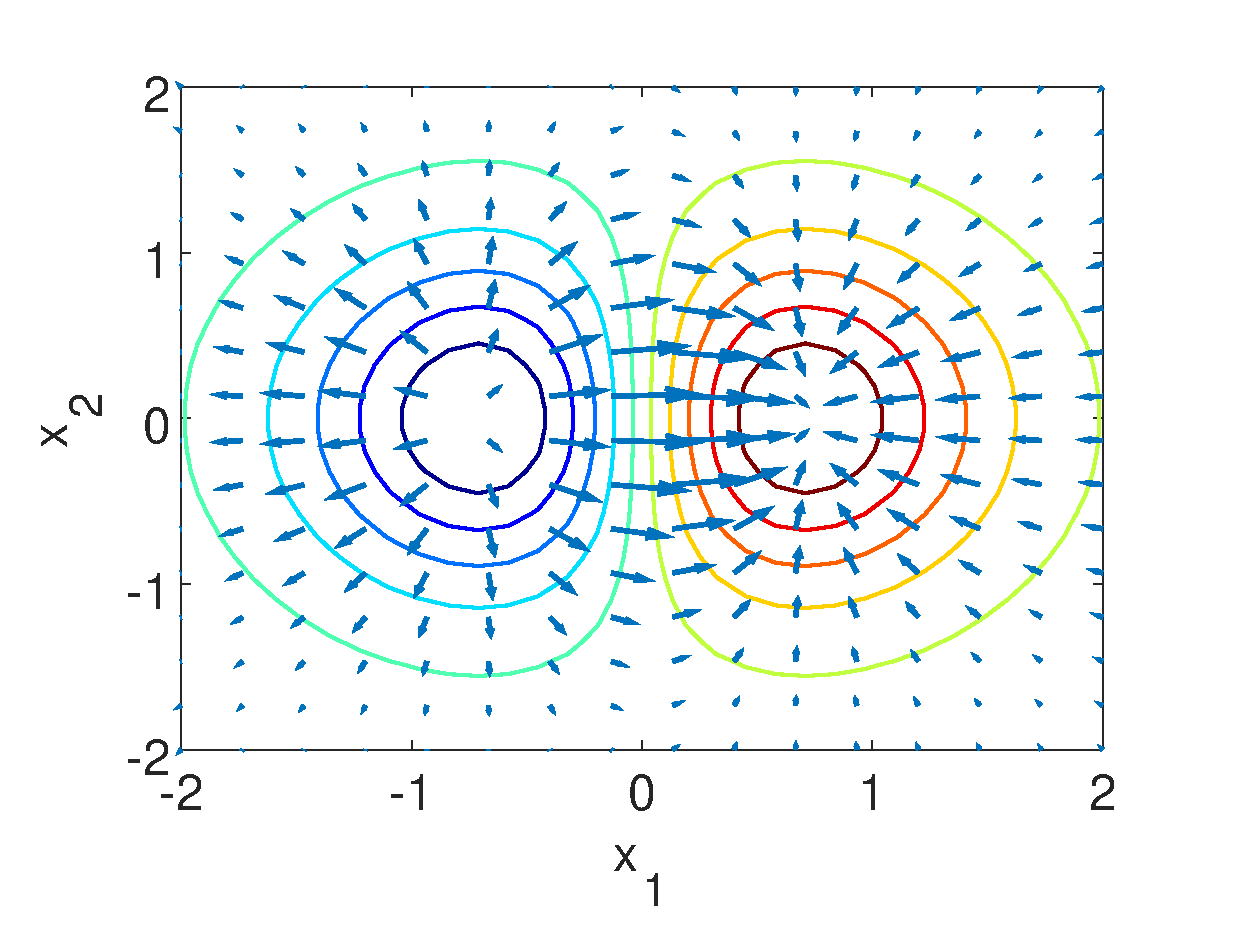
\includegraphics[width=\textwidth]{chapters/derivada/mfiles/gradiente/gradient.eps}
        \caption{Gráfico de $e(\VECTOR{x})$ como curvas de nível e $\triangledown e(\VECTOR{x})$ como vetores.}
        \label{fig:ex:gradient}
    \end{figure}
\end{minipage}

%%%%%%%%%%%%%%%%%%%%%%%%%%%%%%%%%%%%%%%%%%%%%%%%%%%%%%%%%%%%%%%%%%%%%%%%%%%%%%%%
\index{Matriz Jacobiana}
\begin{proposition}[Matriz Jacobiana de $\VECTOR{f}(\VECTOR{x})$:]\label{def:jacobian}
 Dado um vetor coluna, como função $\VECTOR{f}:\mathbb{R}^{N}\rightarrow \mathbb{R}^{M}$ com variável $\VECTOR{x} \in \mathbb{R}^{N}$
 como vetor coluna com elementos $x_n\in \mathbb{R}$ de modo que $n\in \mathbb{N}$, $1 \leq n \leq N$,
 diferenciável em $\VECTOR{x}$. 
 $\MATRIX{J}(\VECTOR{x})$ é chamada matriz Jacobiana \cite[pp. 130]{zhang2017matrix} \cite{Jacobian}  de 
 $\VECTOR{f}(\VECTOR{x})=[f_1(\VECTOR{x})~f_2(\VECTOR{x})~\dots~f_m(\VECTOR{x})~\dots f_M(\VECTOR{x})]^{\transpose}$, de modo que: 
 \begin{equation}
   \frac{\partial \VECTOR{f}(\VECTOR{x})}{\partial \VECTOR{x}^{\transpose} }=
\left[
\begin{matrix}
\frac{\partial \VECTOR{f}(\VECTOR{x}) }{\partial x_{1}}&
\frac{\partial \VECTOR{f}(\VECTOR{x}) }{\partial x_{2}}&
\hdots&
\frac{\partial \VECTOR{f}(\VECTOR{x}) }{\partial x_{n}}&
\hdots&
\frac{\partial \VECTOR{f}(\VECTOR{x}) }{\partial x_{N}}
\end{matrix}
\right]
 \end{equation}

\begin{equation}
\MATRIX{J}(\VECTOR{x})\equiv
\left[\overrightarrow{\triangledown} \VECTOR{f}^{\transpose}(\VECTOR{x})\right]^{\transpose} \equiv 
\frac{\partial \VECTOR{f}(\VECTOR{x})}{\partial \VECTOR{x}^{\transpose} }
\end{equation}

  \begin{equation}
  \MATRIX{J}(\VECTOR{x})\equiv 
\left[
\begin{matrix}
\frac{\partial f_1(\VECTOR{x}) }{\partial x_{1}}&
\frac{\partial f_1(\VECTOR{x}) }{\partial x_{2}}&
\hdots&
\frac{\partial f_1(\VECTOR{x}) }{\partial x_{n}}&
\hdots&
\frac{\partial f_1(\VECTOR{x}) }{\partial x_{N}}\\
\frac{\partial f_2(\VECTOR{x}) }{\partial x_{1}}&
\frac{\partial f_2(\VECTOR{x}) }{\partial x_{2}}&
\hdots&
\frac{\partial f_2(\VECTOR{x}) }{\partial x_{n}}&
\hdots&
\frac{\partial f_2(\VECTOR{x}) }{\partial x_{N}}\\
\vdots&
\vdots&
\hdots&
\vdots&
\vdots&
\vdots\\
\frac{\partial f_m(\VECTOR{x}) }{\partial x_{1}}&
\frac{\partial f_m(\VECTOR{x}) }{\partial x_{2}}&
\hdots&
\frac{\partial f_m(\VECTOR{x}) }{\partial x_{n}}&
\hdots&
\frac{\partial f_m(\VECTOR{x}) }{\partial x_{N}}\\
\vdots&
\vdots&
\hdots&
\vdots&
\vdots&
\vdots\\
\frac{\partial f_M(\VECTOR{x}) }{\partial x_{1}}&
\frac{\partial f_M(\VECTOR{x}) }{\partial x_{2}}&
\hdots&
\frac{\partial f_M(\VECTOR{x}) }{\partial x_{n}}&
\hdots&
\frac{\partial f_M(\VECTOR{x}) }{\partial x_{N}}\\
\end{matrix}
\right]
 \end{equation}
\end{proposition}


\begin{example}[Uso da Proposição \ref{def:jacobian}:]
Conhecida a função $\VECTOR{f}: \mathbb{R}^2 \rightarrow \mathbb{R}^2$,
onde $\VECTOR{u}=\VECTOR{f}(\VECTOR{x})$, 
\begin{equation}
\VECTOR{f}(\VECTOR{x})=
\begin{bmatrix}
\frac{x_1^3+x_2}{5}\\
\frac{x_2^3+x_1}{5}
\end{bmatrix}
\qquad \rightarrow \qquad
\frac{\partial \VECTOR{f}(\VECTOR{x}) }{\partial \VECTOR{x}^{\transpose}}\equiv
\MATRIX{J}(\VECTOR{x})\equiv
\begin{bmatrix}
\VECTOR{j}_{u_1}(\VECTOR{x})\\
\VECTOR{j}_{u_2}(\VECTOR{x})
\end{bmatrix}\equiv
\begin{bmatrix}
\frac{3 x_1^2}{5} & \frac{1}{5}\\
\frac{1}{5}       & \frac{3 x_2^2}{5}
\end{bmatrix}.
\end{equation}
Se $\VECTOR{\hat{x}}=[1~ 1]^{\transpose}$, usando a função $\VECTOR{f}(\VECTOR{\hat{x}})$ 
podemos calcular que $\VECTOR{\hat{u}}=[0.4~ 0.4]^{\transpose}$;
e usando a função $\MATRIX{J}(\VECTOR{\hat{x}})$ obtemos que $\VECTOR{j}_{u_1}(\VECTOR{\hat{x}})=[0.6~ 0.2]$ e $\VECTOR{j}_{u_2}(\VECTOR{\hat{x}})=[0.2~ 0.6]$.
Um gráfico do uso da matriz jacobiana avaliada em $\MATRIX{J}([1~ 1]^{\transpose})$ pode ser visto na Figura \ref{fig:ex:jacobiano}.
\end{example}

\begin{figure}[!h]
    \centering
    \begin{subfigure}[b]{0.49\textwidth}
        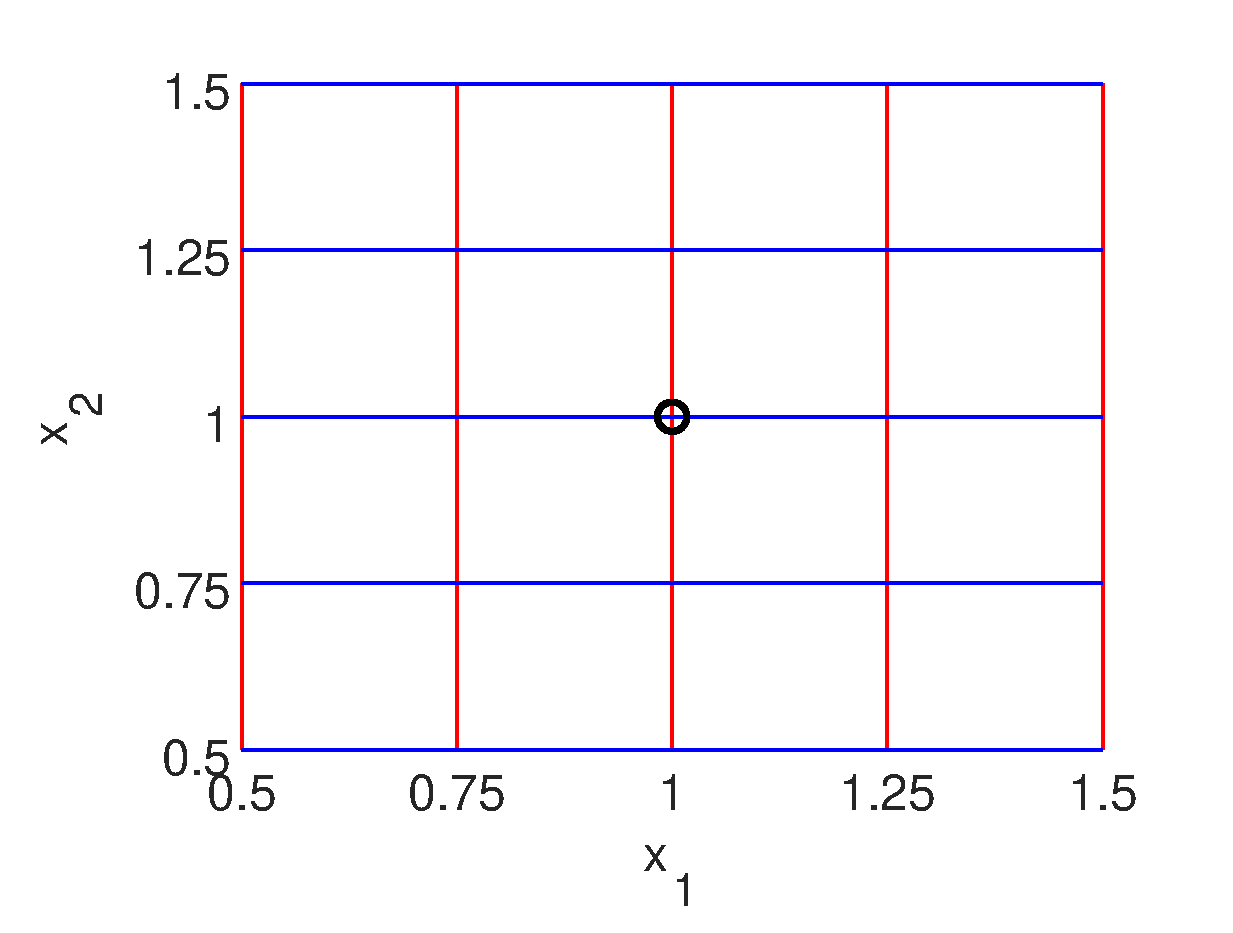
\includegraphics[width=\textwidth]{chapters/derivada/mfiles/jacobian/jacobian1.eps}
        \caption{Gráfico do ponto $\VECTOR{\hat{x}}$ e linhas auxiliares. ~~~~~~~~~ ~~~~~~~~~ ~~~~~~~~~}
        \label{fig:ex:jacobiano:x}
    \end{subfigure}
    ~ %add desired spacing between images, e. g. ~, \quad, \qquad, \hfill etc. 
      %(or a blank line to force the subfigure onto a new line)
    \begin{subfigure}[b]{0.49\textwidth}
        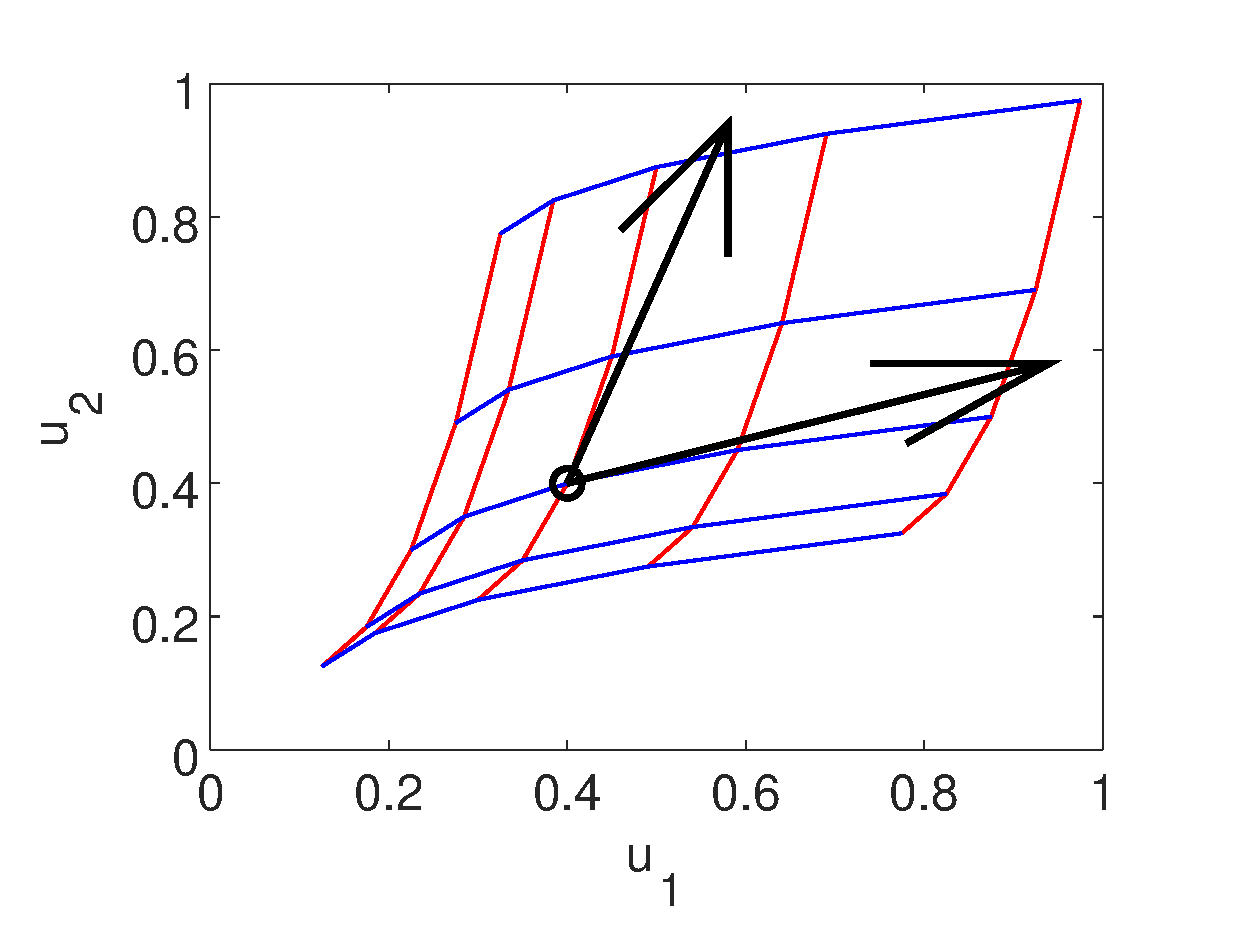
\includegraphics[width=\textwidth]{chapters/derivada/mfiles/jacobian/jacobian2.eps}
        \caption{Gráfico do ponto $\VECTOR{\hat{u}}$, dos vetores $\VECTOR{j}_{u_1}(\VECTOR{\hat{x}})$ e
    $\VECTOR{j}_{u_2}(\VECTOR{\hat{x}})$, e da avaliação das linhas auxiliares na função $\VECTOR{f}$.}
        \label{fig:ex:jacobiano:u}
    \end{subfigure}
    \caption{Gráfico do uso da matriz jacobiana.}
    \label{fig:ex:jacobiano}
\end{figure}


%%%%%%%%%%%%%%%%%%%%%%%%%%%%%%%%%%%%%%%%%%%%%%%%%%%%%%%%%%%%%%%%%%%%%%%%%%%%%%%%
\begin{proposition}[$\triangledown^2 e(\VECTOR{x})$ - Matriz Hessiana de $e(\VECTOR{x})$:]\label{def:hessian}
 Dada uma função $e:\mathbb{R}^{N}\rightarrow \mathbb{R}$ com variável $\VECTOR{x} \in \mathbb{R}^{N}$
 como vetor coluna  com elementos $x_n\in \mathbb{R}$ de modo que $n\in \mathbb{N}$, $1 \leq n \leq N$,
 diferenciável em $\VECTOR{x}$. 
 $\MATRIX{H}(\VECTOR{x})$ é chamada matriz Hessiana \cite[pp. 150]{zhang2017matrix} \cite{Hessian} 
 de $e(\VECTOR{x})$, de modo que: 
\begin{equation}
  \MATRIX{H}(\VECTOR{x}) \equiv  \overrightarrow{\triangledown} \overrightarrow{\triangledown}^{\transpose}e(\VECTOR{x}) \equiv  
\triangledown^2 e(\VECTOR{x}) \equiv \frac{\partial }{\partial \VECTOR{x}} \left( \frac{\partial e(\VECTOR{x})}{ \partial \VECTOR{x}^{\transpose} }\right) 
\end{equation}
 \begin{equation}
  \MATRIX{H}(\VECTOR{x}) =
\left[
\begin{matrix}
\frac{\partial^2 e(\VECTOR{x}) }{\partial x_{1}\partial x_{1}}&
\frac{\partial^2 e(\VECTOR{x}) }{\partial x_{1}\partial x_{2}}&
\hdots&
\frac{\partial^2 e(\VECTOR{x}) }{\partial x_{1}\partial x_{n}}&
\hdots&
\frac{\partial^2 e(\VECTOR{x}) }{\partial x_{1}\partial x_{N}}\\
\frac{\partial^2 e(\VECTOR{x}) }{\partial x_{2}\partial x_{1}}&
\frac{\partial^2 e(\VECTOR{x}) }{\partial x_{2}\partial x_{2}}&
\hdots&
\frac{\partial^2 e(\VECTOR{x}) }{\partial x_{2}\partial x_{n}}&
\hdots&
\frac{\partial^2 e(\VECTOR{x}) }{\partial x_{2}\partial x_{N}}\\
\vdots&
\vdots&
\vdots&
\vdots&
\vdots&
\vdots\\
\frac{\partial^2 e(\VECTOR{x}) }{\partial x_{m}\partial x_{1}}&
\frac{\partial^2 e(\VECTOR{x}) }{\partial x_{m}\partial x_{2}}&
\hdots&
\frac{\partial^2 e(\VECTOR{x}) }{\partial x_{m}\partial x_{n}}&
\hdots&
\frac{\partial^2 e(\VECTOR{x}) }{\partial x_{m}\partial x_{N}}\\
\vdots&
\vdots&
\vdots&
\vdots&
\vdots&
\vdots\\
\frac{\partial^2 e(\VECTOR{x}) }{\partial x_{M}\partial x_{1}}&
\frac{\partial^2 e(\VECTOR{x}) }{\partial x_{M}\partial x_{2}}&
\hdots&
\frac{\partial^2 e(\VECTOR{x}) }{\partial x_{M}\partial x_{n}}&
\hdots&
\frac{\partial^2 e(\VECTOR{x}) }{\partial x_{M}\partial x_{N}}\\
\end{matrix}
\right]
 \end{equation}
\end{proposition}
\index{Matriz Hessiana}



%%%%%%%%%%%%%%%%%%%%%%%%%%%%%%%%%%%%%%%%%%%%%%%%%%%%%%%%%%%%%%%%%%%%%%%%%%%%%%%%
\newpage

%%%%%%%%%%%%%%%%%%%%%%%%%%%%%%%%%%%%%%%%%%%%%%%%%%%%%%%%%%%%%%%%%%%%%%%%%%%%%%%%%%%%%%%
%%%%%%%%%%%%%%%%%%%%%%%%%%%%%%%%%%%%%%%%%%%%%%%%%%%%%%%%%%%%%%%%%%%%%%%%%%%%%%%%%%%%%%%
%%%%%%%%%%%%%%%%%%%%%%%%%%%%%%%%%%%%%%%%%%%%%%%%%%%%%%%%%%%%%%%%%%%%%%%%%%%%%%%%%%%%%%%
\section{Série de Taylor de $f(x)$, $\VECTOR{f}(x)$, $e(\VECTOR{x})$ e $\VECTOR{f}(\VECTOR{x})$}
\label{def:taylor}


\index{Série de Taylor!$f:\mathbb{R} \rightarrow \mathbb{R}$}
\begin{proposition}[Série de Taylor de $f(x)$:]\label{prop:taylord}
Dada uma função $f:\mathbb{R}\rightarrow \mathbb{R}$ com variável $x \in \mathbb{R}$,
infinitamente diferenciável em $a \in \mathbb{R}$;
esta pode ser expressada mediante uma somatória, em série de Taylor 
\cite[pp. 734]{stewart2008calculus} \cite[pp. 281]{telles2015matematica} \cite{Taylor} 
ao redor de $a$, como
mostra a Eq. (\ref{eq:taylord1}),% onde $\left.\frac{\partial^k f(x)}{\partial x^k}\right|_{x=a}\equiv f^{(k)}(a) $.
\begin{equation}\label{eq:taylord0a}
\left.\frac{\partial^k f(x)}{\partial x^k}\right|_{x=a}\equiv f^{(k)}(a) 
\end{equation}
\begin{equation}\label{eq:taylord1}
  f(x)=f(a)
      ~+\frac{f'(a)}{1!} (x-a)
      ~+\frac{f''(a)}{2!} (x-a)^{2}
      ~+\cdots 
      ~+\frac{f^{(k)}(a)}{k!} (x-a)^{k}
      ~+\cdots 
\end{equation}
A equação pode ser escrita de forma mais compacta mediante uma somatória, como mostra a Eq. (\ref{eq:taylord2}),
\begin{equation}\label{eq:taylord2}
  f(x)=\sum\limits_{k=0}^{+\infty} \frac{f^{(k)}(a)}{k!} (x-a)^{k}.
\end{equation}
\end{proposition}

\begin{proposition}[Polinômio de Taylor com resto $R_n(x)$ de Lagrange:]\label{prop:polytaylor}
Dada uma função $f:\mathbb{R}\rightarrow \mathbb{R}$ com variável $x \in \mathbb{R}$;
esta pode ser expressada mediante uma somatória finita, $f_n(x)$, 
em polinômio de Taylor de grau $n$ ao redor de $a$
\cite[pp. 737]{stewart2008calculus} \cite[pp. 285]{telles2015matematica}, 
 como mostra a Eq. (\ref{eq:polytaylord1}),
\begin{equation}\label{eq:polytaylord1}
  f_n(x)=\sum\limits_{k=0}^{n} \frac{f^{(k)}(a)}{k!} (x-a)^{k},
\qquad
R_n(x)=\frac{f^{(n+1)}(z)}{(n+1)!} (x-a)^{n+1},
\end{equation}
\begin{equation}\label{eq:polytaylord2}
f(x)= f_n(x) + R_n(x);
\end{equation}
onde $z \in ]a,x[$, quando $x>a$, e $z \in ]x,a[$, quando $x<a$.
\end{proposition}


\begin{example}[Polinômio de Taylor do $cos(x)$:]
Aproximar a função $f(x)=cos(x)$ usando o polinômio de Taylor ao redor do ponto $a=0$,
numa versão truncada ate a derivada de ordem $4$, $8$ e $10$,
denominados aqui $f_4(x)$, $f_8(x)$ e $f_{10}(x)$, respetivamente.
\end{example}
\begin{SolutionT}[Série de Taylor do $cos(x)$:]
Usando a Proposição \ref{prop:taylord} é calculado $f^{(k)}(x)$ para os 10 primeiros termos,
\begin{equation}
f^{(k)}(x)=
\left\{
\begin{matrix}
cos(x) & ~if & (k~mod~4)=0\\
-sin(x)& ~if & (k~mod~4)=1\\
-cos(x)& ~if & (k~mod~4)=2\\
sin(x) & ~if & (k~mod~4)=3
\end{matrix}
\right.
\quad \rightarrow \quad
f^{(k)}(0)=
\left\{
\begin{matrix}
1 & ~if & (k~mod~4)=0\\
0& ~if & (k~mod~4)=1\\
-1& ~if & (k~mod~4)=2\\
0 & ~if & (k~mod~4)=3
\end{matrix}
\right.
\end{equation}

\begin{equation}
f_{4}(x)=
1
-\frac{x^{2}}{2!} 
+\frac{x^{4}}{4!},
\qquad 
f_{8}(x)=
1
-\frac{x^{2}}{2!} 
+\frac{x^{4}}{4!} 
-\frac{x^{6}}{6!} 
+\frac{x^{8}}{8!}, 
\end{equation}
\begin{equation}
f_{10}(x)=
1
-\frac{x^{2}}{2!} 
+\frac{x^{4}}{4!} 
-\frac{x^{6}}{6!} 
+\frac{x^{8}}{8!} 
-\frac{x^{10}}{10!} 
\end{equation}
As aproximações podem ser vistas graficamente na Fig. \ref{fig:taylore}.
\end{SolutionT}

\begin{figure}[!h]
  \centering
    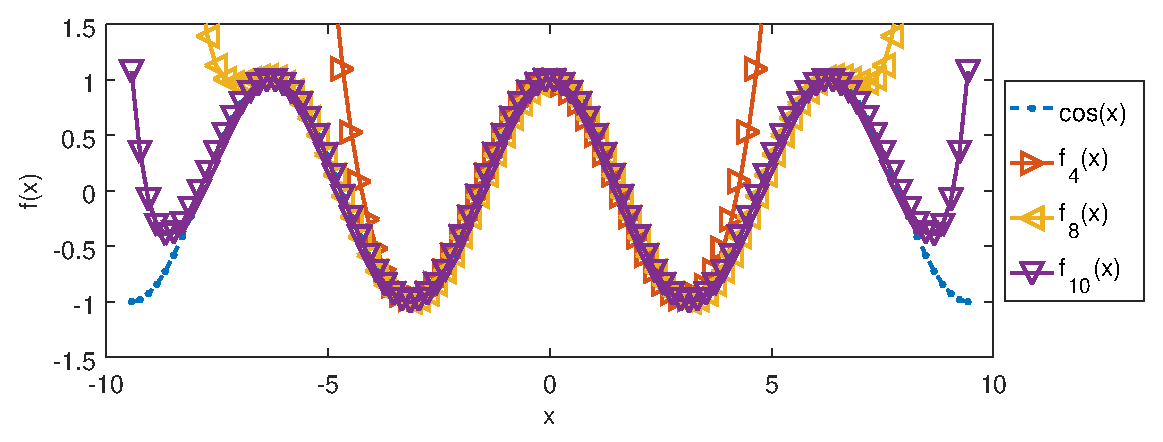
\includegraphics[width=0.90\textwidth]{chapters/funcoes/mcode/taylorR1R1/taylore.eps}
  \caption{Aproximação da função $cos(x)$ usando a série de Taylor truncada.}
    \label{fig:taylore}
\end{figure}
 


%%%%%%%%%%%%%%%%%%%%%%%%%%%%%%%%%%%%%%%%%%%%%%%%%%%%%%%%%%%%%%%%%%%%%%%%%%%%%%%%
\index{Série de Taylor!$\VECTOR{f}:\mathbb{R} \rightarrow \mathbb{R}^{N}$}
\begin{proposition}[Série de Taylor de $\VECTOR{f}(t)$:]\label{prop:taylorvecf}
Dada uma função $\VECTOR{f}:\mathbb{R}\rightarrow \mathbb{R}^{N}$ com variável $t \in \mathbb{R}$;
infinitamente diferenciável em $a \in \mathbb{R}$;
esta pode ser expressada mediante uma somatória, em série de Taylor 
\cite[pp. 264]{joag2016introduction}
ao redor de $a$, como
mostra a Eq. (\ref{eq:taylorvecf1}),
\begin{equation}\label{eq:taylorvecf0a}
\left.\frac{\partial^k \VECTOR{f}(t)}{\partial t^k}\right|_{t=a}\equiv \VECTOR{f}^{(k)}(a) 
\end{equation}
\begin{equation}\label{eq:taylorvecf1}
  \VECTOR{f}(t)=\VECTOR{f}(a)
      ~+\frac{\DTVECTOR{f}(a)}{1!} (t-a)
      ~+\frac{\DDTVECTOR{f}(a)}{2!} (t-a)^{2}
      ~+\cdots 
      ~+\frac{\VECTOR{f}^{(k)}(a)}{k!} (t-a)^{k}
      ~+\cdots 
\end{equation}
A equação pode ser escrita de forma mais compacta mediante uma somatória  como mostra a Eq. (\ref{eq:taylorvecf2}),
\begin{equation}\label{eq:taylorvecf2}
  \VECTOR{f}(t)=\sum\limits_{k=0}^{+\infty} \frac{\VECTOR{f}^{(k)}(a)}{k!} (t-a)^{k}.
\end{equation}
\end{proposition}

\begin{example}[Polinômio de Taylor de ordem 4 de uma função vetorial:]\label{ex:prop:taylorvecf}
Aproximar a função $\VECTOR{f}:\mathbb{R} \rightarrow \mathbb{R}^{2}$,
\begin{equation}
\VECTOR{f}(t)=
\begin{bmatrix}
cos(t)\\
e^{-t}
\end{bmatrix},
\end{equation}
usando o polinômio de Taylor ao redor do ponto $a=0$,
numa versão truncada ate a derivada de ordem $4$,
denominado aqui $\VECTOR{f}_4(x)$.
\end{example}
\begin{SolutionT}[Relativo ao Exemplo \ref{ex:prop:taylorvecf}:]
Usando a Proposição \ref{prop:taylorvecf} são calculados os vetores $\VECTOR{f}^{(k)}(x)$, para $k\in\{1,~ 2,~ 3,~ 4\}$,
de modo que obtemos
\begin{equation}
\DTVECTOR{f}(t)=
\begin{bmatrix}
-sin(t)\\
-e^{-t}
\end{bmatrix},~
\DDTVECTOR{f}(t)=
\begin{bmatrix}
-cos(t)\\
e^{-t}
\end{bmatrix},~
\DDDTVECTOR{f}(t)=
\begin{bmatrix}
sin(t)\\
-e^{-t}
\end{bmatrix},~
\DDDDTVECTOR{f}(t)=
\begin{bmatrix}
cos(t)\\
e^{-t}
\end{bmatrix},
\end{equation}
\begin{equation}
\VECTOR{f}(0)=
\begin{bmatrix}
1\\
1
\end{bmatrix},
\quad
\DTVECTOR{f}(0)=
\begin{bmatrix}
0\\
-1
\end{bmatrix},
\quad
\DDTVECTOR{f}(0)=
\begin{bmatrix}
-1\\
1
\end{bmatrix},
\quad
\DDDTVECTOR{f}(0)=
\begin{bmatrix}
0\\
-1
\end{bmatrix},
\quad
\DDDDTVECTOR{f}(0)=
\begin{bmatrix}
1\\
1
\end{bmatrix}.
\end{equation}
Podemos agrupar estas informações na Eq. (\ref{eq:taylorvecf1}) truncada, 
para obter o polinômio $\VECTOR{f}_{4}(t)$,
\begin{equation}
\VECTOR{f}_{4}(t)=
\begin{bmatrix}
1\\
1
\end{bmatrix}
+
\begin{bmatrix}
0\\
-1
\end{bmatrix}
t
+
\begin{bmatrix}
-1\\
1
\end{bmatrix}
\frac{t^{2}}{2!}
+
\begin{bmatrix}
0\\
-1
\end{bmatrix}
\frac{t^{3}}{3!}
+
\begin{bmatrix}
1\\
1
\end{bmatrix}
\frac{t^{4}}{4!}.
\end{equation}
Uma representação gráfica do comportamento do polinômio $\VECTOR{f}_{4}(t)$ e a função $\VECTOR{f}(t)$
pode ser visto na Figura \ref{fig:taylorvecf}.
\end{SolutionT}

\begin{figure}[!h]
  \centering
    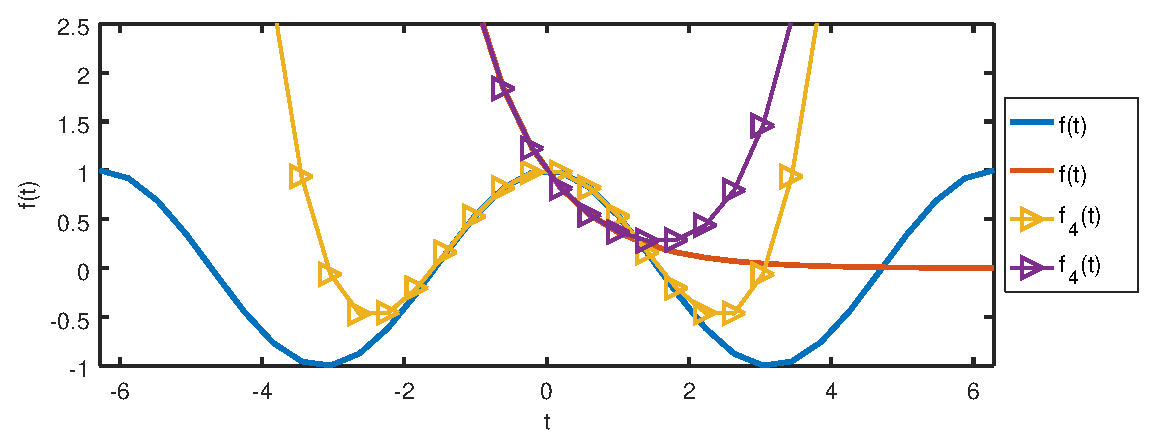
\includegraphics[width=0.90\textwidth]{chapters/funcoes/mcode/taylorR1R2/taylore.eps}
  \caption{Aproximação da função da função $\VECTOR{f}(t)$ mediante o polinômio $\VECTOR{f}_{4}(t)$.}
    \label{fig:taylorvecf}
\end{figure}

%%%%%%%%%%%%%%%%%%%%%%%%%%%%%%%%%%%%%%%%%%%%%%%%%%%%%%%%%%%%%%%%%%%%%%%%%%%%%%%%%%%%%%%
\index{Série de Taylor!$f:\mathbb{R}^{N}\rightarrow \mathbb{R}$}
\begin{proposition}[Série de Taylor de $f(\VECTOR{x})$:]\label{prop:taylore}
Dada uma função $f:\mathbb{R}^{N}\rightarrow \mathbb{R}$ com variável $\VECTOR{x} \in \mathbb{R}^{N}$, vetor coluna;
infinitamente diferenciável em $\VECTOR{a} \in \mathbb{R}^{N}$;
esta pode ser expressada mediante uma somatória, em série de Taylor 
\cite[pp. 187, 207]{zhang2017matrix} \cite{Taylor}  ao redor de $\VECTOR{a}$, como
mostra a Eq. (\ref{eq:taylore1}),
\begin{equation}\label{eq:taylore1}
f(\VECTOR{x}) =\sum _{k_{1}=0}^{\infty }\cdots \sum _{k_{N}=0}^{\infty }\left.\left({\frac {\partial ^{k_{1}+\cdots +k_{N}}f(\VECTOR{x})}{\partial x_{1}^{k_{1}}\cdots \partial x_{N}^{k_{N}}}}\right)\right|_{\VECTOR{x}=\VECTOR{a}} {\frac {(x_{1}-a_{1})^{k_{1}}\cdots (x_{N}-a_{N})^{k_{N}}}{k_{1}!\cdots k_{N}!}}
\end{equation}

Outra forma alternativa de expressar a função anterior é usando vetores e matrizes,
como na Eq. (\ref{eq:taylore2}).
\begin{equation}\label{eq:taylore2}
  f(\VECTOR{x})=f(\VECTOR{a})
      ~+ \triangledown f(\VECTOR{a})^{\transpose} (\VECTOR{x}-\VECTOR{a})
      ~+\frac{1}{2!}(\VECTOR{x}-\VECTOR{a})^{\transpose} \MATRIX{H(\VECTOR{a})}  (\VECTOR{x}-\VECTOR{a})
      ~+\cdots 
\end{equation}
Onde o vector $\triangledown f(\VECTOR{x})\equiv \frac{\partial f(\VECTOR{x})}{\partial \VECTOR{x} }$ 
(também chamado \hyperref[def:gradient]{gradiente}),
e a matriz $\MATRIX{H}(\VECTOR{x})\equiv \frac{\partial }{\partial \VECTOR{x}} \left( \frac{\partial f(\VECTOR{x})}{ \partial \VECTOR{x}^{\transpose} }\right)$
(também chamada matriz \hyperref[def:hessian]{Hessiana}).
\end{proposition}

\begin{example}[Série de Taylor do 
$f(\VECTOR{x})$:]
Aproximar a função $f(\VECTOR{x})=1-e^{-x_1^2-x_2^2}$ usando a série de Taylor ao redor do ponto $\VECTOR{a}=[0~ 0]^{\transpose}$,
numa versão truncada ate a derivada de ordem $2$,
denominada aqui $f_2(\VECTOR{x})$.
\end{example}
\begin{SolutionT}[Série de Taylor do 
$f(\VECTOR{x})$:]
Usando a Proposição \ref{prop:taylore} é calculado $f(\VECTOR{a})$, 
$\triangledown f(\VECTOR{a})$ e $\triangledown^2 f(\VECTOR{a})$,
\begin{equation}
\triangledown f(\VECTOR{x}) = 
2 e^{-x_1^2-x_2^2}
\begin{bmatrix}
x_1 \\
x_2
\end{bmatrix},
\qquad 
\triangledown^2 f(\VECTOR{x}) = 
-2 e^{-x_1^2-x_2^2}
\begin{bmatrix}
2 x_1^2-1 & 2 x_1 x_2\\
2 x_1 x_2 & 2 x_2^2-1
\end{bmatrix}.
\end{equation}
Avaliando o ponto $\VECTOR{a}$,
\begin{equation}
f(\VECTOR{a})=0,
\qquad 
\triangledown f(\VECTOR{a}) = 
\begin{bmatrix}
0 \\
0
\end{bmatrix},
\qquad 
\triangledown^2 f(\VECTOR{a}) = 
\begin{bmatrix}
2 & 0\\
0 & 2
\end{bmatrix},
\qquad 
f_2(\VECTOR{x}) = 
\VECTOR{x}^{\transpose}\VECTOR{x}.
\end{equation}
As aproximações podem ser vistas graficamente na Fig. \ref{fig:taylorf}.
\end{SolutionT}


\begin{figure}[!h]
  \centering
    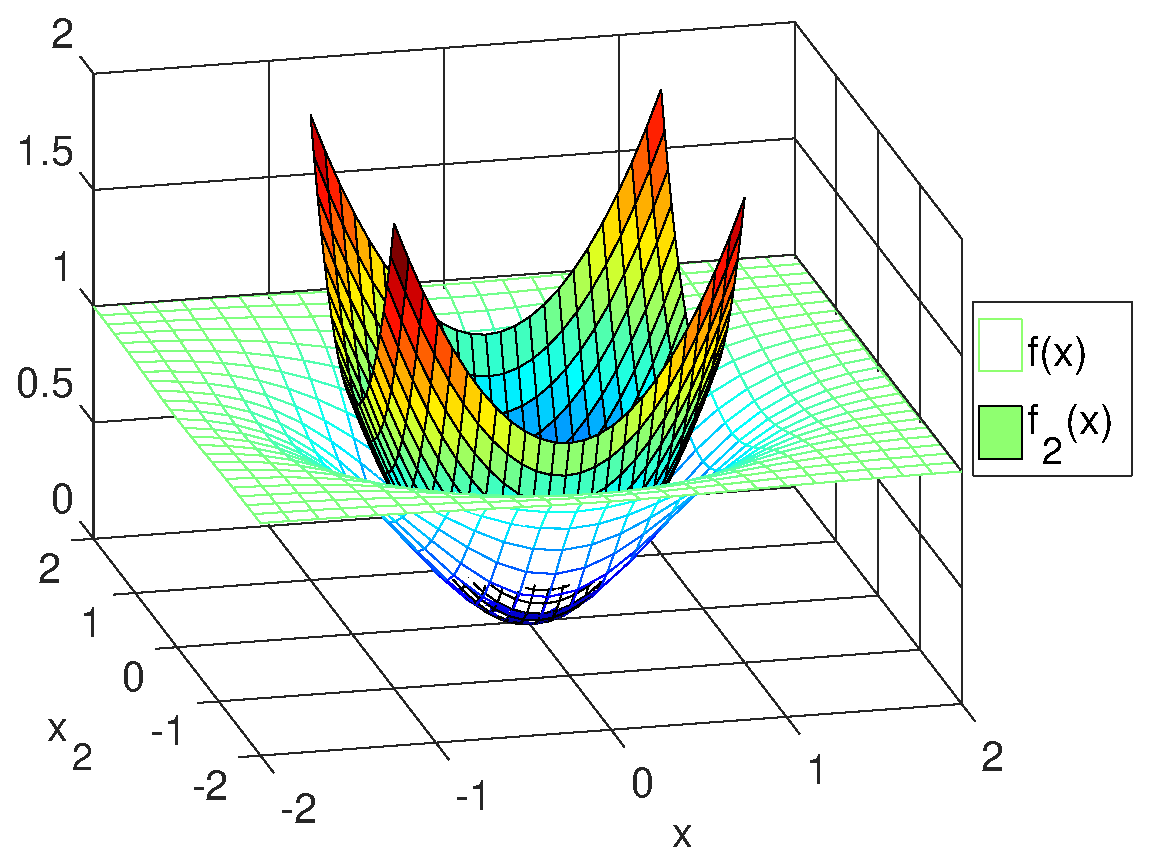
\includegraphics[width=0.5\textwidth]{chapters/funcoes/mcode/taylorR2R1/taylorf.eps}
  \caption{Aproximação $f_2(\VECTOR{x})$ da função $f(\VECTOR{x})$.}
    \label{fig:taylorf}
\end{figure}
 
%%%%%%%%%%%%%%%%%%%%%%%%%%%%%%%%%%%%%%%%%%%%%%%%%%%%%%%%%%%%%%%%%%%%%%%%%%%%%%%%%%%%%%%
\index{Série de Taylor!$\VECTOR{f}:\mathbb{R}^{N}\rightarrow \mathbb{R}^{M}$}
\begin{proposition}[Série de Taylor de $\VECTOR{f}(\VECTOR{x})$:]\label{prop:taylorf}
Dada uma função  $\VECTOR{f}:\mathbb{R}^{N}\rightarrow \mathbb{R}^{M}$, 
sendo $\VECTOR{f}$ um vector coluna com variável $\VECTOR{x} \in \mathbb{R}^{N}$, vetor coluna;
infinitamente diferenciável em $\VECTOR{a} \in \mathbb{R}^{N}$;
esta pode ser expressada mediante uma somatória, em série de Taylor 
\cite[pp. 393]{levine1999control} \cite{Taylor} ao redor de $\VECTOR{a}$, como
mostra a Eq. (\ref{eq:taylorf1}),
\begin{equation}\label{eq:taylorf1}
\VECTOR{f}(\VECTOR{x}) =\VECTOR{f}(\VECTOR{a})
      ~+ \MATRIX{J}(\VECTOR{a}) (\VECTOR{x}-\VECTOR{a})
      ~+\cdots 
\end{equation}

Onde a matriz $\MATRIX{J}(\VECTOR{x})\equiv \frac{\partial \VECTOR{f}(\VECTOR{x})}{\partial \VECTOR{x}^{\transpose} }$,
também conhecido como matriz \hyperref[def:jacobian]{Jacobiana} de $\VECTOR{f}(\VECTOR{x})$.
\end{proposition}


\index{Taylor, Brook}
\begin{elaboracion}[title=Brook Taylor (1685-1731), width= 0.99\linewidth]
Matemático inglês que foi um dos fundadores do cálculo das diferenças finitas,
sendo ele o primeiro a reconhecer a existência de soluções singulares de equações diferenciais.
A série Taylor, era conhecida por James Gregory quando Taylor tinha apenas alguns anos de idade. 
Acredita-se que Taylor não conhecia o trabalho de Gregory quando publicou seu livro ``Methodus incrementorum directa et inversa'' (1715),
que continha a série Taylor \cite[pp. 198]{agarwal2014creators}.
\end{elaboracion}




%----------------------------------------------------------------------------------------
%	CHAPTER  
%----------------------------------------------------------------------------------------
\chapterimage{chapter_derivada.pdf} % Chapter heading image

\chapter{Derivada de funções: $\mathbb{R}^{N}$ $\rightarrow$ $\mathbb{R}^{M}$}


%%%%%%%%%%%%%%%%%%%%%%%%%%%%%%%%%%%%%%%%%%%%%%%%%%%%%%%%%%%%%%%%%%%%%%%%%%%%%%%%%%%%%%%
%%%%%%%%%%%%%%%%%%%%%%%%%%%%%%%%%%%%%%%%%%%%%%%%%%%%%%%%%%%%%%%%%%%%%%%%%%%%%%%%%%%%%%%
\section{Derivada de $\MATRIX{A}\VECTOR{x}$}

\begin{theorem}\label{theo:derAx}
Se 
$\VECTOR{x}\in \mathbb{R}^N$ é um vetor coluna com elementos $x_n$ de modo que
$n\in \mathbb{N}$, $1 \leq n \leq N$, e 
$\MATRIX{A} \in \mathbb{R}^{M\times N}$ é uma matriz com elementos $a_{mn}$ de modo que
$m\in \mathbb{N}$, $1 \leq m \leq M$, então se cumpre que:
\begin{equation}
\frac{\partial \MATRIX{A}\VECTOR{x}}{\partial x_n}=a_{:n}
\end{equation}
A demostração pode ser vista na Prova \ref{proof:theo:derAx}.
\end{theorem}

\begin{corollaryT}[Derivada de $\MATRIX{A}\VECTOR{x}$ em relação ao vector $\VECTOR{x}^{\transpose}$]\label{coro:derAx1}
Aplicando a Definição \ref{def:deltahor} junto ao Teorema \ref{theo:derAx}, é
fácil deduzir que:
\begin{equation}
\frac{\partial \MATRIX{A}\VECTOR{x}}{\partial \VECTOR{x}^{\transpose}}=
\MATRIX{A}=
\left[
\begin{matrix}
 a_{:1} &  a_{:2} &  \cdots &  a_{:N}
\end{matrix}
\right]
\end{equation}
\end{corollaryT}

\begin{corollaryT}[Derivada de $\MATRIX{A}\VECTOR{x}$ em relação ao vector $\VECTOR{x}$]\label{coro:derAx2}
Aplicando a Definição \ref{def:deltaver} junto ao Teorema \ref{theo:derAx}, é
fácil deduzir que:
\begin{equation}
\frac{\partial \MATRIX{A}\VECTOR{x}}{\partial \VECTOR{x}}=\funcvec(\MATRIX{A})=
\left[
\begin{matrix}
 a_{:1} \\  a_{:2} \\  \vdots \\  a_{:N}
\end{matrix}
\right]
\end{equation}
\end{corollaryT}

\begin{corollaryT}[Derivada de $\VECTOR{a}^{\transpose}\VECTOR{x}$ em relação ao vector $\VECTOR{x}^{\transpose}$]\label{coro:derAx3}
Aplicando a Definição \ref{def:deltahor} junto ao Teorema \ref{theo:derAx} e sabendo que $\VECTOR{a}^{\transpose}$
é um vetor linha, é
fácil deduzir que:
\begin{equation}
\frac{\partial \VECTOR{a}^{\transpose}\VECTOR{x}}{\partial \VECTOR{x}^{\transpose}}=\VECTOR{a}^{\transpose}
\end{equation}
\end{corollaryT}

\begin{corollaryT}[Derivada de $\VECTOR{a}^{\transpose}\VECTOR{x}$ em relação ao vector $\VECTOR{x}$]\label{coro:derAx4}
Aplicando a Definição \ref{def:deltaver} junto ao Teorema \ref{theo:derAx} e sabendo que $\VECTOR{a}^{\transpose}$
é um vetor linha, é
fácil deduzir que:
\begin{equation}
\frac{\partial \VECTOR{a}^{\transpose}\VECTOR{x}}{\partial \VECTOR{x}}=\VECTOR{a}
\end{equation}
\end{corollaryT}

%%%%%%%%%%%%%%%%%%%%%%%%%%%%%%%%%%%%%%%%%%%%%%%%%%%%%%%%%%%%%%%%%%%%%%%%%%%%%%%%%%%%%%%
%%%%%%%%%%%%%%%%%%%%%%%%%%%%%%%%%%%%%%%%%%%%%%%%%%%%%%%%%%%%%%%%%%%%%%%%%%%%%%%%%%%%%%%
\section{Derivada de $||\MATRIX{A}\VECTOR{x}||^2$ 
}

\begin{theorem}\label{theo:derxAtAx}
Se 
$\VECTOR{x}\in \mathbb{R}^N$ é um vetor coluna com elementos $x_n$ de modo que
$n\in \mathbb{N}$, $1 \leq n \leq N$, e 
$\MATRIX{A} \in \mathbb{R}^{M\times N}$ é uma matriz com elementos $a_{mn}$ de modo que
$m\in \mathbb{N}$, $1 \leq m \leq M$, então se cumpre que:
\begin{equation}
\begin{matrix}
\frac{\partial ||\MATRIX{A}\VECTOR{x}||^2 }{\partial x_n}&=&
\frac{\partial \left(\MATRIX{A}\VECTOR{x}\right)^{\transpose}\left(\MATRIX{A}\VECTOR{x}\right)}{\partial x_n}&=&
2\left(\MATRIX{A}\VECTOR{x}\right)^{\transpose}a_{:n}\\
~&~&~&=& 2\left(a_{:n}\right)^{\transpose}\MATRIX{A}\VECTOR{x}
\end{matrix}
\end{equation}
A demostração pode ser vista na Prova \ref{proof:theo:derxAtAx}.
\end{theorem}

\begin{corollaryT}[Derivada de $||\MATRIX{A}\VECTOR{x}||^2$ em relação ao vector $\VECTOR{x}^{\transpose}$]\label{coro:derxAtAx1}
Aplicando a Definição \ref{def:deltahor} junto ao Teorema \ref{theo:derxAtAx}, é
fácil deduzir que:
\begin{equation}
\frac{\partial ||\MATRIX{A}\VECTOR{x}||^2 }{\partial \VECTOR{x}^{\transpose}}=
2\left(\MATRIX{A}^{\transpose}\MATRIX{A}\VECTOR{x}\right)^{\transpose}
\end{equation}
%\frac{\partial \left(\MATRIX{A}\VECTOR{x}\right)^{\transpose}\left(\MATRIX{A}\VECTOR{x}\right)}{\partial \VECTOR{x}^{\transpose}}=
\end{corollaryT}

\begin{corollaryT}[Derivada de $||\MATRIX{A}\VECTOR{x}||^2$ em relação ao vector $\VECTOR{x}$]\label{coro:derxAtAx2}
Aplicando a Definição \ref{def:deltaver} junto ao Teorema \ref{theo:derxAtAx}, é
fácil deduzir que:
\begin{equation}
\frac{\partial ||\MATRIX{A}\VECTOR{x}||^2 }{\partial \VECTOR{x}}=
2 \MATRIX{A}^{\transpose}\MATRIX{A}\VECTOR{x}
\end{equation}
%\frac{\partial \left(\MATRIX{A}\VECTOR{x}\right)^{\transpose}\left(\MATRIX{A}\VECTOR{x}\right)}{\partial \VECTOR{x}}=
\end{corollaryT}

%%%%%%%%%%%%%%%%%%%%%%%%%%%%%%%%%%%%%%%%%%%%%%%%%%%%%%%%%%%%%%%%%%%%%%%%%%%%%%%%%%%%%%%
%%%%%%%%%%%%%%%%%%%%%%%%%%%%%%%%%%%%%%%%%%%%%%%%%%%%%%%%%%%%%%%%%%%%%%%%%%%%%%%%%%%%%%%
\section{Derivada de $||\MATRIX{A}\VECTOR{x}-\VECTOR{b}||_{\MATRIX{C}}^2$ 
}

\begin{theorem}\label{theo:derAxbAxb}
Se 
$\VECTOR{x}\in \mathbb{R}^N$ é um vetor coluna com elementos $x_n$ de modo que
$n\in \mathbb{N}$, $1 \leq n \leq N$, 
$\VECTOR{b}\in \mathbb{R}^M$ é um vetor coluna com elementos $b_m$ de modo que
$m\in \mathbb{N}$, $1 \leq m \leq M$,  
$\MATRIX{A} \in \mathbb{R}^{M\times N}$ é uma matriz com elementos $a_{mn}$, e
$\MATRIX{C} \in \mathbb{R}^{M\times M}$ é uma matriz diagonal, 
então se cumpre que:
\begin{equation}
\begin{matrix}
\frac{\partial ||\MATRIX{A}\VECTOR{x}-\VECTOR{b}||_{\MATRIX{C}}^2}{\partial x_n}&=&
\frac{\partial \left(\MATRIX{A}\VECTOR{x}-\VECTOR{b}\right)^{\transpose}\MATRIX{C}\left(\MATRIX{A}\VECTOR{x}-\VECTOR{b}\right)}{\partial x_n}&=&
2\left(\MATRIX{A}\VECTOR{x}-\VECTOR{b}\right)^{\transpose}\MATRIX{C}a_{:n}\\
~&~&~&=& 2\left(a_{:n}\right)^{\transpose}\MATRIX{C}\left(\MATRIX{A}\VECTOR{x}-  \VECTOR{b}\right)
\end{matrix}
\end{equation}
A demostração pode ser vista na Prova \ref{proof:theo:derAxbAxb}.
\end{theorem}

\begin{corollaryT}[Derivada de $||\MATRIX{A}\VECTOR{x}-\VECTOR{b}||_{\MATRIX{C}}^2$ em relação ao vector $\VECTOR{x}^{\transpose}$]\label{coro:derAxbAxb1}
Aplicando a Definição \ref{def:deltahor} junto ao Teorema \ref{theo:derAxbAxb}, é
fácil deduzir que:
\begin{equation}
\frac{\partial ||\MATRIX{A}\VECTOR{x}-\VECTOR{b}||_{\MATRIX{C}}^2}{\partial \VECTOR{x}^{\transpose}}=
2\left(\MATRIX{A}\VECTOR{x}- \VECTOR{b} \right)^{\transpose}\MATRIX{C}\MATRIX{A}
\end{equation}
\end{corollaryT}

\begin{corollaryT}[Derivada de $||\MATRIX{A}\VECTOR{x}-\VECTOR{b}||_{\MATRIX{C}}^2$ em relação ao vector $\VECTOR{x}$]\label{coro:derAxbAxb2}
Aplicando a Definição \ref{def:deltaver} junto ao Teorema \ref{theo:derAxbAxb}, é
fácil deduzir que:
\begin{equation}
\frac{\partial ||\MATRIX{A}\VECTOR{x}-\VECTOR{b}||_{\MATRIX{C}}^2}{\partial \VECTOR{x} }=
2 \MATRIX{A}^{\transpose}\MATRIX{C}\left(\MATRIX{A}\VECTOR{x}-\VECTOR{b}\right)
\end{equation}
\end{corollaryT}

%%%%%%%%%%%%%%%%%%%%%%%%%%%%%%%%%%%%%%%%%%%%%%%%%%%%%%%%%%%%%%%%%%%%%%%%%%%%%%%%%%%%%%%
%%%%%%%%%%%%%%%%%%%%%%%%%%%%%%%%%%%%%%%%%%%%%%%%%%%%%%%%%%%%%%%%%%%%%%%%%%%%%%%%%%%%%%%
\section{Derivada de $||\VECTOR{f}(\VECTOR{x})-\VECTOR{b}||_{\MATRIX{C}}^2$  
}

\begin{theorem}[Valor exato:]\label{theo:derfxbCfxb0}
Se 
$\VECTOR{x}\in \mathbb{R}^N$ e, 
$\VECTOR{b}\in \mathbb{R}^M$ são vetores coluna,  
$\VECTOR{f}: \mathbb{R}^{N}\rightarrow \mathbb{R}^{M}$ é uma função de valor vectorial, e
$\MATRIX{C} \in \mathbb{R}^{M\times M}$ é uma matriz diagonal, 
então se cumpre que:
\begin{equation}
\frac{\partial ||\VECTOR{f}(\VECTOR{x})-\VECTOR{b}||_{\MATRIX{C}}^2}{\partial \VECTOR{x}} =
2 \MATRIX{J}(\VECTOR{x})^{\transpose}\MATRIX{C}\left[\VECTOR{f}(\VECTOR{x})-\VECTOR{b}\right],
\end{equation}
onde $\MATRIX{J}(\VECTOR{x})$ é a \hyperref[def:jacobian]{\textbf{matriz Jacobiana}} de $\VECTOR{f}(\VECTOR{x})$.

A demostração pode ser vista na Prova \ref{proof:theo:derfxbCfxb0}.
\end{theorem}

\begin{theorem}[Valor aproximado:]\label{theo:derfxbCfxb}
Se 
$\VECTOR{x}\in \mathbb{R}^N$ é um vetor coluna, 
$\VECTOR{b}\in \mathbb{R}^M$ é um vetor coluna,  
$\VECTOR{f}: \mathbb{R}^{N}\rightarrow \mathbb{R}^{M}$ é uma função de valor vectorial, e
$\MATRIX{C} \in \mathbb{R}^{M\times M}$ é uma matriz diagonal, 
então se cumpre que:
\begin{equation}
\frac{\partial ||\VECTOR{f}(\VECTOR{x})-\VECTOR{b}||_{\MATRIX{C}}^2}{\partial \VECTOR{x}} \approx
2 \MATRIX{J}(\VECTOR{p})^{\transpose}\MATRIX{C}\left[\MATRIX{J}(\VECTOR{p})\left(\VECTOR{x} - \VECTOR{p}\right)-\left(\VECTOR{b}-\VECTOR{f}(\VECTOR{p})\right)\right]
\end{equation}

Onde é considerada a aproximação
$\VECTOR{f}(\VECTOR{x})\approx \VECTOR{f}(\VECTOR{p})+\MATRIX{J}(\VECTOR{p})\left(\VECTOR{x}-\VECTOR{p}\right)$,
usando a \hyperref[def:taylor]{\textbf{serie de Taylor}} para funções multivariáveis. Sendo $\VECTOR{p}$ um ponto fixo no domínio de $\VECTOR{f}(\VECTOR{x})$,  ao redor do qual é feita  aproximação
da função $\VECTOR{f}(\VECTOR{x})$,
e $\MATRIX{J}(\VECTOR{p})$ é a \hyperref[def:jacobian]{\textbf{matriz Jacobiana}} de $\VECTOR{f}(\VECTOR{x})$ avaliado no ponto $\VECTOR{p}$.

A demostração pode ser vista na Prova \ref{proof:theo:derfxbCfxb}.
\end{theorem}



%%%%%%%%%%%%%%%%%%%%%%%%%%%%%%%%%%%%%%%%%%%%%%%%%%%%%%%%%%%%%%%%%%%%%%%%%%%%%%%%%%%%%%%
%%%%%%%%%%%%%%%%%%%%%%%%%%%%%%%%%%%%%%%%%%%%%%%%%%%%%%%%%%%%%%%%%%%%%%%%%%%%%%%%%%%%%%%
\section{Derivada de $||\VECTOR{f}(\VECTOR{x})-\VECTOR{b}||_{\MATRIX{C}}^2+\alpha||\VECTOR{x}-\VECTOR{q}||_{\MATRIX{D}}^2$ 
}

\begin{theorem}[Valor exato:]\label{theo:exact:derfxbCfxbxqDxq}
Se 
$\VECTOR{x}\in \mathbb{R}^N$,
$\VECTOR{q}\in \mathbb{R}^N$ e, 
$\VECTOR{b}\in \mathbb{R}^M$ são vetores coluna,  
$\VECTOR{f}: \mathbb{R}^{N}\rightarrow \mathbb{R}^{M}$ é uma função de valor vectorial, e
$\MATRIX{C} \in \mathbb{R}^{M\times M}$ e $\MATRIX{D} \in \mathbb{R}^{N\times N}$ são matrizes diagonais, 
então se cumpre\footnote{A 
demostração pode ser vista na união da Prova \ref{proof:theo:derfxbCfxb0} e o Corolário \ref{coro:derAxbAxb2}.} que:
\begin{equation}
\frac{\partial ||\VECTOR{f}(\VECTOR{x})-\VECTOR{b}||_{\MATRIX{C}}^2+\alpha||\VECTOR{x}-\VECTOR{q}||_{\MATRIX{D}}^2}{\partial \VECTOR{x}} 
= 2 \MATRIX{J}(\VECTOR{x})^{\transpose}\MATRIX{C}\left[\VECTOR{f}(\VECTOR{x})-\VECTOR{b}\right]
+ 2 \alpha\MATRIX{D}\left(\VECTOR{x}-\VECTOR{q}\right),
\end{equation}
onde $\MATRIX{J}(\VECTOR{x})$ é a \hyperref[def:jacobian]{\textbf{matriz Jacobiana}} de $\VECTOR{f}(\VECTOR{x})$.
\end{theorem}



\begin{theorem}[Valor aproximado:]\label{theo:derfxbCfxbxqDxq}
Se 
$\VECTOR{x}\in \mathbb{R}^N$ é um vetor coluna, 
$\VECTOR{b}\in \mathbb{R}^M$ é um vetor coluna,
$\VECTOR{q}\in \mathbb{R}^N$ é um vetor coluna, 
$\VECTOR{f}: \mathbb{R}^{N}\rightarrow \mathbb{R}^{M}$ é uma função de valor vectorial, 
$\MATRIX{C} \in \mathbb{R}^{M\times M}$ é uma matriz diagonal, e
$\MATRIX{D} \in \mathbb{R}^{N\times N}$ é uma matriz diagonal, 
então se cumpre\footnote{A demostração pode ser vista na Prova \ref{proof:theo:derfxbCfxbxqDxq}.} que:
\begin{equation}
\frac{\partial \left(||\VECTOR{f}(\VECTOR{x})-\VECTOR{b}||_{\MATRIX{C}}^2+\alpha||\VECTOR{x}-\VECTOR{q}||_{\MATRIX{D}}^2\right)}{\partial \VECTOR{x}} \approx
2 \MATRIX{J}(\VECTOR{p})^{\transpose}\MATRIX{C}\left\{\MATRIX{J}(\VECTOR{p})\left[\VECTOR{x} - \VECTOR{p}\right]-\left[\VECTOR{b}-\VECTOR{f}(\VECTOR{p})\right] \right\}
+2\alpha\MATRIX{D}\left[\VECTOR{x}-\VECTOR{q}\right]
\end{equation}

Onde é considerada a aproximação
$\VECTOR{f}(\VECTOR{x})\approx \VECTOR{f}(\VECTOR{p})+\MATRIX{J}(\VECTOR{p})\left(\VECTOR{x}-\VECTOR{p}\right)$,
usando a \hyperref[def:taylor]{\textbf{serie de Taylor}} para funções multivariáveis. Sendo $\VECTOR{p}$ um ponto fixo no domínio de $\VECTOR{f}(\VECTOR{x})$,  ao redor do qual é feita  aproximação
da função $\VECTOR{f}(\VECTOR{x})$,
e $\MATRIX{J}(\VECTOR{p})$ é a matriz \hyperref[def:jacobian]{Jacobiana} \cite{Jacobian} de $\VECTOR{f}(\VECTOR{x})$ avaliado no ponto $\VECTOR{p}$.


\end{theorem}


%%%%%%%%%%%%%%%%%%%%%%%%%%%%%%%%%%%%%%%%%%%%%%%%%%%%%%%%%%%%%%%%%%%%%%%%%%%%%%%%%%%%%%%
%%%%%%%%%%%%%%%%%%%%%%%%%%%%%%%%%%%%%%%%%%%%%%%%%%%%%%%%%%%%%%%%%%%%%%%%%%%%%%%%%%%%%%%
\section{Derivada de segundo ordem de $||\VECTOR{f}(\VECTOR{x})-\VECTOR{b}||_{\MATRIX{C}}^2$ 
}



\begin{theorem}[Valor exato:]\label{theo:der2fxbCfxb0}
Se
$\VECTOR{x}\in \mathbb{R}^N$ e 
$\VECTOR{b}\in \mathbb{R}^M$ são vetores coluna,  
$\VECTOR{f}: \mathbb{R}^{N}\rightarrow \mathbb{R}^{M}$ é uma função de valor vectorial,
$\MATRIX{C} \in \mathbb{R}^{M\times M}$ é uma matriz diagonal, e
definimos a função $e(\VECTOR{x})$ como
\begin{equation}
e(\VECTOR{x})= ||\VECTOR{f}(\VECTOR{x})-\VECTOR{b}||_{\MATRIX{C}}^2.
\end{equation}
Então a \hyperref[def:hessian]{\textbf{matriz Hessiana}} $\MATRIX{H}(\VECTOR{x})$ 
de $e(\VECTOR{x})$ é igual\footnote{A demostração pode ser vista na Prova \ref{proof:theo:der2fxbCfxb0}.} a:
\begin{equation}
\MATRIX{H}(\VECTOR{x}) = \frac{\partial}{\partial \VECTOR{x}^{\transpose}}\left(  
\frac{\partial e(\VECTOR{x}) }{\partial \VECTOR{x}} \right) = 2 \MATRIX{B}(\VECTOR{x})
+2 \MATRIX{J}(\VECTOR{x})^{\transpose}\MATRIX{C} \MATRIX{J}(\VECTOR{x}),
\end{equation}
onde 
\begin{equation}
 \MATRIX{B}(\VECTOR{x})=
{\bigcup\limits_{n=1}^{ \rightarrow }}^{N}\left\{ \frac{\partial \MATRIX{J}(\VECTOR{x})^{\transpose} }{\partial x_{n}} \MATRIX{C} \left( \VECTOR{f}(\VECTOR{x})-\VECTOR{b}\right) \right\},
\end{equation}
\end{theorem}

\begin{theorem}[Valor aproximado:]\label{theo:der2fxbCfxb0aprox}
Se 
$\VECTOR{x}\in \mathbb{R}^N$ é  
$\VECTOR{b}\in \mathbb{R}^M$ são vetores coluna,  
$\VECTOR{f}: \mathbb{R}^{N}\rightarrow \mathbb{R}^{M}$ é uma função de valor vectorial,
$\MATRIX{C} \in \mathbb{R}^{M\times M}$ é uma matriz diagonal, e 
definimos a função $e(\VECTOR{x})$ como
\begin{equation}
e(\VECTOR{x})= ||\VECTOR{f}(\VECTOR{x})-\VECTOR{b}||_{\MATRIX{C}}^2.
\end{equation}
Então, para achar uma forma aproximada da \hyperref[def:hessian]{\textbf{matriz Hessiana}} $\MATRIX{H}(\VECTOR{x})$ de $e(\VECTOR{x})$, 
podemos usar a aproximação linear de $\VECTOR{f}(\VECTOR{x})$ por meio da \hyperref[def:taylor]{\textbf{serie de Taylor}} 
para funções multivariáveis\footnote{ $\VECTOR{f}(\VECTOR{x})\approx \VECTOR{f}(\VECTOR{p}) + \MATRIX{J}(\VECTOR{p})$ $\left(\VECTOR{x}-\VECTOR{p}\right)$,
onde $\VECTOR{p}$ é um ponto fixo no domínio de $\VECTOR{f}(\VECTOR{x})$ ao redor do qual é feita  aproximação
da função $\VECTOR{f}(\VECTOR{x})$,
e $\MATRIX{J}(\VECTOR{p})$ é a \hyperref[def:jacobian]{\textbf{matriz Jacobiana}} de $\VECTOR{f}(\VECTOR{x})$ avaliada no ponto $\VECTOR{p}$.}, obtendo\footnote{A demostração pode ser vista na Prova \ref{proof:theo:der2fxbCfxb0aprox}.} o seguinte resultado,
\begin{equation}
\MATRIX{H}(\VECTOR{x}) = \frac{\partial}{\partial \VECTOR{x}^{\transpose}}\left(  
\frac{\partial e(\VECTOR{x}) }{\partial \VECTOR{x}} \right) \approx 
2 \MATRIX{J}(\VECTOR{p})^{\transpose}\MATRIX{C} \MATRIX{J}(\VECTOR{p}).
\end{equation}


\end{theorem}



\section{Provas dos teoremas}

%%%%%%%%%%%%%%%%%%%%%%%%%%%%%%%%%%%%%%%%%%%%%%%%%%%%%%%%%%%%%%%%%%%%%%%%%%%%%%%%%%%%%%%
%%%%%%%%%%%%%%%%%%%%%%%%%%%%%%%%%%%%%%%%%%%%%%%%%%%%%%%%%%%%%%%%%%%%%%%%%%%%%%%%%%%%%%%
\begin{myproofT}[Relativa ao Teorema \ref{theo:derAx}:]\label{proof:theo:derAx}
Dados,
uma matriz $\MATRIX{A}=\left[a_{:1}~ a_{:2}~ \hdots~ a_{:n}~ \hdots~ a_{:N}\right]$ e 
um vetor coluna $\VECTOR{x}=\left[x_{1}~ x_{2}~ \hdots~ x_{n}~ \hdots~ x_{N}\right]^{\transpose}$, 
podemos expressar que:
\begin{equation}
\frac{\partial \MATRIX{A}\VECTOR{x}}{\partial x_n}=
\frac{\partial \MATRIX{A}}{\partial x_n}\VECTOR{x}+\MATRIX{A}\frac{\partial \VECTOR{x}}{\partial x_n}=
\MATRIX{A}\frac{\partial \VECTOR{x}}{\partial x_n}.
\end{equation}
Sabendo que $\frac{\partial \VECTOR{x}}{\partial x_n}$ é igual a um vetor 
com um $1$ na posição $n$ e $0$ em qualquer outra posição, obtemos que
\begin{equation}
\frac{\partial \MATRIX{A}\VECTOR{x}}{\partial x_n}=
\left[a_{:1}~ a_{:2}~ \hdots~ a_{:n}~ \hdots~ a_{:N}\right]\left[
\begin{matrix}
 0\\
 0\\
 \vdots\\
 1\\
 \vdots\\
 0
\end{matrix}
\right]=a_{:n}.
\end{equation}
\end{myproofT}

%%%%%%%%%%%%%%%%%%%%%%%%%%%%%%%%%%%%%%%%%%%%%%%%%%%%%%%%%%%%%%%%%%%%%%%%%%%%%%%%%%%%%%%
%%%%%%%%%%%%%%%%%%%%%%%%%%%%%%%%%%%%%%%%%%%%%%%%%%%%%%%%%%%%%%%%%%%%%%%%%%%%%%%%%%%%%%%
\begin{myproofT}[Relativa ao Teorema \ref{theo:derxAtAx}:]\label{proof:theo:derxAtAx}
Dados,
uma matriz $\MATRIX{A}=\left[a_{:1}~ a_{:2}~ \hdots~ a_{:n}~ \hdots~ a_{:N}\right]$ e 
um vetor coluna $\VECTOR{x}=\left[x_{1}~ x_{2}~ \hdots~ x_{n}~ \hdots~ x_{N}\right]^{\transpose}$, 
podemos expressar que:
\begin{equation}\label{eq:proof:derxAtAx1}
\frac{\partial ||\MATRIX{A}\VECTOR{x}||^{2}}{\partial x_n}=
\frac{\partial \left(\MATRIX{A}\VECTOR{x}\right)^{\transpose}\left(\MATRIX{A}\VECTOR{x}\right)}{\partial x_n}=
\left(\frac{\partial \MATRIX{A}\VECTOR{x}}{\partial x_n}\right)^{\transpose}\left(\MATRIX{A}\VECTOR{x}\right)+
\left(\MATRIX{A}\VECTOR{x}\right)^{\transpose} \frac{\partial \MATRIX{A}\VECTOR{x}}{\partial x_n}.
\end{equation}
Pelo visto no Teorema \ref{theo:derAx} podemos substituir valores na Eq. (\ref{eq:proof:derxAtAx1})
e obter:
\begin{equation}\label{eq:proof:derxAtAx2}
\frac{\partial ||\MATRIX{A}\VECTOR{x}||^{2}}{\partial x_n}=
\left(a_{:n}\right)^{\transpose} \MATRIX{A}\VECTOR{x} +
\left(\MATRIX{A}\VECTOR{x}\right)^{\transpose} a_{:n}.
\end{equation}
Como cada um dos somandos da equação anterior é um escalar, podemos aplicar o operador
transposta ($\transpose$) sobre qualquer somando sem alterar o resultado; de modo que temos duas possíveis
forma de expressar a solução:
\begin{equation}
\begin{matrix}
\frac{\partial ||\MATRIX{A}\VECTOR{x}||^2 }{\partial x_n}&=&
2\left(\MATRIX{A}\VECTOR{x}\right)^{\transpose}a_{:n}\\
~&=& 2\left(a_{:n}\right)^{\transpose}\MATRIX{A}\VECTOR{x}.
\end{matrix}
\end{equation}
\end{myproofT}

%%%%%%%%%%%%%%%%%%%%%%%%%%%%%%%%%%%%%%%%%%%%%%%%%%%%%%%%%%%%%%%%%%%%%%%%%%%%%%%%%%%%%%%
%%%%%%%%%%%%%%%%%%%%%%%%%%%%%%%%%%%%%%%%%%%%%%%%%%%%%%%%%%%%%%%%%%%%%%%%%%%%%%%%%%%%%%%
\begin{myproofT}[Relativa ao Teorema \ref{theo:derAxbAxb}:]\label{proof:theo:derAxbAxb}
Dados,
uma matriz $\MATRIX{A}=\left[a_{:1}~ a_{:2}~ \hdots~ a_{:n}~ \hdots~ a_{:N}\right]$, 
uma matriz diagonal $\MATRIX{C}\in \mathbb{R}^{M\times M}$, 
um vetor coluna $\VECTOR{x}=\left[x_{1}~ x_{2}~ \hdots~ x_{n}~ \hdots~ x_{N}\right]^{\transpose}$, e 
um vetor coluna $\VECTOR{b}\in \mathbb{R}^{M}$, 
podemos expressar que:
\begin{equation}\label{eq:proof:derAxbAxb1}
\frac{\partial ||\MATRIX{A}\VECTOR{x}-\VECTOR{b}||_{\MATRIX{C}}^2}{\partial x_n} =
\frac{\partial \left(\MATRIX{A}\VECTOR{x}-\VECTOR{b}\right)^{\transpose}\MATRIX{C}\left(\MATRIX{A}\VECTOR{x}-\VECTOR{b}\right)}{\partial x_n}=
 \left(\frac{\partial\MATRIX{A}\VECTOR{x}}{\partial x_n}\right)^{\transpose}\MATRIX{C}\left(\MATRIX{A}\VECTOR{x}-\VECTOR{b}\right)+
 \left(\MATRIX{A}\VECTOR{x}-\VECTOR{b}\right)^{\transpose}\MATRIX{C}\left(\frac{\partial\MATRIX{A}\VECTOR{x}}{\partial x_n}\right).
\end{equation}
Pelo visto no Teorema \ref{theo:derAx}, podemos substituir valores na Eq. (\ref{eq:proof:derAxbAxb1})
e obter:
\begin{equation}\label{eq:proof:derAxbAxb2}
\frac{\partial ||\MATRIX{A}\VECTOR{x}-\VECTOR{b}||_{\MATRIX{C}}^{2}}{\partial x_n}=
\left(a_{:n}\right)^{\transpose}\MATRIX{C}\left( \MATRIX{A}\VECTOR{x}-\VECTOR{b}\right) +
\left(\MATRIX{A}\VECTOR{x}-\VECTOR{b}\right)^{\transpose}\MATRIX{C} a_{:n}.
\end{equation}
Como cada um dos somandos da equação anterior é um escalar, podemos aplicar o operador
transposta ($\transpose$) sobre qualquer somando sem alterar o resultado; de modo que temos duas possíveis
forma de expressar a solução:
\begin{equation}
\begin{matrix}
\frac{\partial ||\MATRIX{A}\VECTOR{x}-\VECTOR{b}||_{\MATRIX{C}}^2 }{\partial x_n}&=&
2\left(\MATRIX{A}\VECTOR{x}-\VECTOR{b}\right)^{\transpose}\MATRIX{C}a_{:n}\\
~&=& 2\left(a_{:n}\right)^{\transpose}\MATRIX{C}\left(\MATRIX{A}\VECTOR{x}-\VECTOR{b}\right).
\end{matrix}
\end{equation}
\end{myproofT}

%%%%%%%%%%%%%%%%%%%%%%%%%%%%%%%%%%%%%%%%%%%%%%%%%%%%%%%%%%%%%%%%%%%%%%%%%%%%%%%%%%%%%%%
%%%%%%%%%%%%%%%%%%%%%%%%%%%%%%%%%%%%%%%%%%%%%%%%%%%%%%%%%%%%%%%%%%%%%%%%%%%%%%%%%%%%%%%
\begin{myproofT}[Relativa ao Teorema \ref{theo:derfxbCfxb0}:]\label{proof:theo:derfxbCfxb0}
Dados,
uma função $\VECTOR{f}:\mathbb{R}^{N} \rightarrow \mathbb{R}^{M}$, 
uma matriz diagonal $\MATRIX{C}\in \mathbb{R}^{M\times M}$, 
um vetor coluna $\VECTOR{x}=\left[x_{1}~ x_{2}~ \hdots~ x_{n}~ \hdots~ x_{N}\right]^{\transpose}$, e
um vetor coluna $\VECTOR{b}\in \mathbb{R}^{M}$;
podemos expressar que:
\begin{equation}\label{eq:proof:derfxbCfxb01}
\begin{matrix}
\frac{\partial ||\VECTOR{f}(\VECTOR{x})-\VECTOR{b}||_{\MATRIX{C}}^2}{\partial x_{n}} & = &
\frac{\partial \left( \VECTOR{f}(\VECTOR{x})-\VECTOR{b}\right)^{\transpose} \MATRIX{C} \left( \VECTOR{f}(\VECTOR{x})-\VECTOR{b}\right) }{\partial x_{n}} \\
~ &= &
 \left(  \frac{\partial\VECTOR{f}(\VECTOR{x})  }{\partial x_{n}} \right)^{\transpose} \MATRIX{C} \left( \VECTOR{f}(\VECTOR{x})-\VECTOR{b}\right) +
 \left( \VECTOR{f}(\VECTOR{x})-\VECTOR{b}\right)^{\transpose} \MATRIX{C}  \left(  \frac{\partial\VECTOR{f}(\VECTOR{x})  }{\partial x_{n}} \right)\\
~ &= &
 2 \left(  \frac{\partial\VECTOR{f}(\VECTOR{x})  }{\partial x_{n}} \right)^{\transpose} \MATRIX{C} \left( \VECTOR{f}(\VECTOR{x})-\VECTOR{b}\right).
\end{matrix}
\end{equation}
Assim, usando a Definição \ref{def:deltaver} junto com a Eq. (\ref{eq:proof:derfxbCfxb01})
nos obtemos:
\begin{equation}\label{eq:proof:derfxbCfxb02}
\frac{\partial ||\VECTOR{f}(\VECTOR{x})-\VECTOR{b}||_{\MATRIX{C}}^2}{\partial \VECTOR{x}}  = 
2 \MATRIX{J}(\VECTOR{x})^{\transpose} \MATRIX{C} \left( \VECTOR{f}(\VECTOR{x})-\VECTOR{b}\right).
\end{equation}
\end{myproofT}


\begin{myproofT}[Relativa ao Teorema \ref{theo:derfxbCfxb}:]\label{proof:theo:derfxbCfxb}
Dados,
uma função $\VECTOR{f}:\mathbb{R}^{N} \rightarrow \mathbb{R}^{M}$, 
uma matriz diagonal $\MATRIX{C}\in \mathbb{R}^{M\times M}$, 
um vetor coluna $\VECTOR{x}\in \mathbb{R}^{N}$, 
um vetor coluna $\VECTOR{b}\in \mathbb{R}^{M}$, 
e considerando a aproximação
$\VECTOR{f}(\VECTOR{x})\approx \VECTOR{f}(\VECTOR{p})+\MATRIX{J}(\VECTOR{p})\left(\VECTOR{x}-\VECTOR{p}\right)$,
obtida a partir da \hyperref[def:taylor]{\textbf{série de Taylor}} para funções multivariáveis;
podemos expressar que:
\begin{equation}\label{eq:proof:derfxbCfxb1}
\frac{\partial ||\VECTOR{f}(\VECTOR{x})-\VECTOR{b}||_{\MATRIX{C}}^2}{\partial \VECTOR{x}} \approx
\frac{\partial ||\MATRIX{J}(\VECTOR{p})\VECTOR{x}-\left[\MATRIX{J}(\VECTOR{p})\VECTOR{p}+\VECTOR{b}-\VECTOR{f}(\VECTOR{p})\right]||_{\MATRIX{C}}^2}{\partial \VECTOR{x}}.
\end{equation}
Pelo visto no Corolário \ref{coro:derAxbAxb2}, podemos substituir os valores,
$\MATRIX{J}(\VECTOR{p})$ e 
$\left[\MATRIX{J}(\VECTOR{p})\VECTOR{p}+\VECTOR{b}-\VECTOR{f}(\VECTOR{p})\right]$,
da Eq. (\ref{eq:proof:derfxbCfxb1}), nas variáveis $\MATRIX{A}$ e $\VECTOR{b}$ 
do Corolário \ref{coro:derAxbAxb2}, respectivamente. Assim obtemos:
\begin{equation}\label{eq:proof:derfxbCfxb2}
\frac{\partial ||\MATRIX{J}(\VECTOR{p})\VECTOR{x}-\left[\MATRIX{J}(\VECTOR{p})\VECTOR{p}+\VECTOR{b}-\VECTOR{f}(\VECTOR{p})\right]||_{\MATRIX{C}}^2}{\partial \VECTOR{x}}  = 
2 \MATRIX{J}(\VECTOR{p})^{\transpose}\MATRIX{C}\left( \MATRIX{J}(\VECTOR{p})\VECTOR{x}-\MATRIX{J}(\VECTOR{p})\VECTOR{p}-\VECTOR{b}+\VECTOR{f}(\VECTOR{p})\right).
\end{equation}
\end{myproofT}


%%%%%%%%%%%%%%%%%%%%%%%%%%%%%%%%%%%%%%%%%%%%%%%%%%%%%%%%%%%%%%%%%%%%%%%%%%%%%%%%%%%%%%%
%%%%%%%%%%%%%%%%%%%%%%%%%%%%%%%%%%%%%%%%%%%%%%%%%%%%%%%%%%%%%%%%%%%%%%%%%%%%%%%%%%%%%%%
\begin{myproofT}[Relativa ao Teorema \ref{theo:der2fxbCfxb0}:]\label{proof:theo:der2fxbCfxb0}
Dados,
uma função $\VECTOR{f}:\mathbb{R}^{N} \rightarrow \mathbb{R}^{M}$, 
uma matriz diagonal $\MATRIX{C}\in \mathbb{R}^{M\times M}$, 
um vetor coluna $\VECTOR{x}=\left[x_{1}~ x_{2}~ \hdots~ x_{n}~ \hdots~ x_{N}\right]^{\transpose}$, e
um vetor coluna $\VECTOR{b}\in \mathbb{R}^{M}$;
podemos expressar que:
\begin{equation}\label{eq:proof:der2fxbCfxb01}
\begin{matrix}
\frac{\partial }{\partial x_{n}}\left( \frac{\partial ||\VECTOR{f}(\VECTOR{x})-\VECTOR{b}||_{\MATRIX{C}}^2}{\partial \VECTOR{x}} \right) & = &
\frac{\partial 2 \MATRIX{J}(\VECTOR{x})^{\transpose} \MATRIX{C} \left( \VECTOR{f}(\VECTOR{x})-\VECTOR{b}\right)}{\partial x_{n}} \\
~ & = & 2 \frac{\partial \MATRIX{J}(\VECTOR{x})^{\transpose} }{\partial x_{n}} \MATRIX{C} \left( \VECTOR{f}(\VECTOR{x})-\VECTOR{b}\right)+
2  \MATRIX{J}(\VECTOR{x})^{\transpose}  \MATRIX{C} \frac{\partial \left( \VECTOR{f}(\VECTOR{x})-\VECTOR{b}\right) }{\partial x_{n}}\\
~ & = & 2 \frac{\partial \MATRIX{J}(\VECTOR{x})^{\transpose} }{\partial x_{n}} \MATRIX{C} \left( \VECTOR{f}(\VECTOR{x})-\VECTOR{b}\right)+
2  \MATRIX{J}(\VECTOR{x})^{\transpose}  \MATRIX{C} \frac{\partial \VECTOR{f}(\VECTOR{x}) }{\partial x_{n}}.\\
\end{matrix}
\end{equation}
Assim, usando a Definição \ref{def:deltahor} junto com a Eq. (\ref{eq:proof:der2fxbCfxb01})
nos obtemos:
\begin{equation}\label{eq:proof:der2fxbCfxb02}
\frac{\partial }{\partial \VECTOR{x}^{\transpose}}\left( \frac{\partial ||\VECTOR{f}(\VECTOR{x})-\VECTOR{b}||_{\MATRIX{C}}^2}{\partial \VECTOR{x}} \right) =
2 {\bigcup\limits_{n=1}^{ \rightarrow }}^{N}\left\{ \frac{\partial \MATRIX{J}(\VECTOR{x})^{\transpose} }{\partial x_{n}} \MATRIX{C} \left( \VECTOR{f}(\VECTOR{x})-\VECTOR{b}\right) \right\} +
2  \MATRIX{J}(\VECTOR{x})^{\transpose}  \MATRIX{C} \frac{\partial \VECTOR{f}(\VECTOR{x}) }{\partial \VECTOR{x}^{\transpose}}.
\end{equation}
\end{myproofT}

\begin{myproofT}[Relativa ao Teorema \ref{theo:der2fxbCfxb0aprox}:]\label{proof:theo:der2fxbCfxb0aprox}
Dados,
uma função $\VECTOR{f}:\mathbb{R}^{N} \rightarrow \mathbb{R}^{M}$, 
uma matriz diagonal $\MATRIX{C}\in \mathbb{R}^{M\times M}$, 
os vetores coluna $\VECTOR{x}\in \mathbb{R}^{N}$ e 
$\VECTOR{b}\in \mathbb{R}^{M}$, e
considerando o Toerema \ref{theo:derfxbCfxb} que usa a aproximação
$\VECTOR{f}(\VECTOR{x})\approx \VECTOR{f}(\VECTOR{p}) + \MATRIX{J}(\VECTOR{p})$ $\left(\VECTOR{x}-\VECTOR{p}\right)$,
podemos expressar que:
\begin{equation}\label{eq:proof:der2fxbCfxb01aprox}
\begin{matrix}
\frac{\partial }{\partial \VECTOR{x}^{\transpose}}\left( \frac{\partial ||\VECTOR{f}(\VECTOR{x})-\VECTOR{b}||_{\MATRIX{C}}^2}{\partial \VECTOR{x}} \right) & \approx & 
\frac{\partial 2 \MATRIX{J}(\VECTOR{p})^{\transpose}\MATRIX{C}\left[\MATRIX{J}(\VECTOR{p})\left(\VECTOR{x} - \VECTOR{p}\right)-\left(\VECTOR{b}-\VECTOR{f}(\VECTOR{p})\right)\right]}{\partial \VECTOR{x}^{\transpose}} \\
~ & \approx & \frac{\partial 2 \MATRIX{J}(\VECTOR{p})^{\transpose}\MATRIX{C} \MATRIX{J}(\VECTOR{p})\VECTOR{x}  }{\partial \VECTOR{x}^{\transpose}}
\end{matrix},
\end{equation}
onde $\VECTOR{p}$ é um ponto fixo no domínio de $\VECTOR{f}(\VECTOR{x})$,  ao redor do qual é feita  aproximação
da função $\VECTOR{f}(\VECTOR{x})$,
e $\MATRIX{J}(\VECTOR{p})$ é a \hyperref[def:jacobian]{\textbf{matriz Jacobiana}} de $\VECTOR{f}(\VECTOR{x})$ avaliado no ponto $\VECTOR{p}$.
Assim, usando o Teorema \ref{theo:derAx} na Eq. (\ref{eq:proof:der2fxbCfxb01aprox})
obtemos,
\begin{equation}\label{eq:proof:der2fxbCfxb01aprox2}
\frac{\partial }{\partial \VECTOR{x}^{\transpose}}\left( \frac{\partial ||\VECTOR{f}(\VECTOR{x})-\VECTOR{b}||_{\MATRIX{C}}^2}{\partial \VECTOR{x}} \right) \approx 
2 \MATRIX{J}(\VECTOR{p})^{\transpose}\MATRIX{C} \MATRIX{J}(\VECTOR{p}).
\end{equation}
\end{myproofT}

%%%%%%%%%%%%%%%%%%%%%%%%%%%%%%%%%%%%%%%%%%%%%%%%%%%%%%%%%%%%%%%%%%%%%%%%%%%%%%%%%%%%%%%
%%%%%%%%%%%%%%%%%%%%%%%%%%%%%%%%%%%%%%%%%%%%%%%%%%%%%%%%%%%%%%%%%%%%%%%%%%%%%%%%%%%%%%%
\begin{myproofT}[Relativa ao Teorema \ref{theo:derfxbCfxbxqDxq}:]\label{proof:theo:derfxbCfxbxqDxq}
Dados,
uma função $\VECTOR{f}:\mathbb{R}^{N} \rightarrow \mathbb{R}^{M}$, 
uma matriz diagonal $\MATRIX{C}\in \mathbb{R}^{M\times M}$, 
uma matriz diagonal $\MATRIX{D}\in \mathbb{R}^{N\times N}$, 
um vetor coluna $\VECTOR{x}\in \mathbb{R}^{N}$, 
um vetor coluna $\VECTOR{b}\in \mathbb{R}^{M}$,e 
um vetor coluna $\VECTOR{q}\in \mathbb{R}^{N}$, 
podemos expressar que:
\begin{equation}\label{eq:proof:derfxbCfxbxqDxq1}
\frac{\partial ||\VECTOR{f}(\VECTOR{x})-\VECTOR{b}||_{\MATRIX{C}}^2 +\alpha||\VECTOR{x}-\VECTOR{q}||_{\MATRIX{D}}^2}{\partial \VECTOR{x}} =
\frac{\partial ||\VECTOR{f}(\VECTOR{x})-\VECTOR{b}||_{\MATRIX{C}}^2}{\partial \VECTOR{x}}+
\alpha \frac{\partial ||\VECTOR{x}-\VECTOR{q}||_{\MATRIX{D}}^2}{\partial \VECTOR{x}}.
\end{equation}
Usando o Corolário \ref{coro:derAxbAxb2} na Eq. (\ref{eq:proof:derfxbCfxbxqDxq1})
obtemos:
\begin{equation}\label{eq:proof:derfxbCfxbxqDxq2}
\frac{\partial ||\VECTOR{f}(\VECTOR{x})-\VECTOR{b}||_{\MATRIX{C}}^2 +\alpha||\VECTOR{x}-\VECTOR{q}||_{\MATRIX{D}}^2}{\partial \VECTOR{x}} =
\frac{\partial ||\VECTOR{f}(\VECTOR{x})-\VECTOR{b}||_{\MATRIX{C}}^2}{\partial \VECTOR{x}}+
\alpha 2 \MATRIX{D}\left(\VECTOR{x}-\VECTOR{q}\right).
\end{equation}
Usando o Teorema \ref{theo:derfxbCfxb} na Eq. (\ref{eq:proof:derfxbCfxbxqDxq2})
obtemos:
\begin{equation}\label{eq:proof:derfxbCfxbxqDxq3}
\frac{\partial ||\VECTOR{f}(\VECTOR{x})-\VECTOR{b}||_{\MATRIX{C}}^2 +\alpha||\VECTOR{x}-\VECTOR{q}||_{\MATRIX{D}}^2}{\partial \VECTOR{x}} \approx
2 \MATRIX{J}(\VECTOR{p})^{\transpose}\MATRIX{C}\left[\MATRIX{J}(\VECTOR{p})\left(\VECTOR{x} - \VECTOR{p}\right)-\left(\VECTOR{b}-\VECTOR{f}(\VECTOR{p})\right)\right]+
2 \alpha \MATRIX{D}\left(\VECTOR{x}-\VECTOR{q}\right).
\end{equation}
\end{myproofT}
%



%----------------------------------------------------------------------------------------
%	PART
%----------------------------------------------------------------------------------------
\part{Problemas de minimização de erro em funções}

%----------------------------------------------------------------------------------------
%	CHAPTER  
%----------------------------------------------------------------------------------------
\chapterimage{chapter_head_2.pdf} % Chapter heading image

\chapter{Minimização do erro em funções: $\mathbb{R}^{N}$ $\rightarrow$ $\mathbb{R}^{M}$}

\begin{remark}
Palavras chave: 
Pseudo-inversa de Moore-Penrose,
regularização de Tikhonov,
problema inverso, 
minimização do erro quadrático. 
\end{remark}

%%%%%%%%%%%%%%%%%%%%%%%%%%%%%%%%%%%%%%%%%%%%%%%%%%%%%%%%%%%%%%%%%%%%%%%%%%%%%%%%%%%%%%%
%%%%%%%%%%%%%%%%%%%%%%%%%%%%%%%%%%%%%%%%%%%%%%%%%%%%%%%%%%%%%%%%%%%%%%%%%%%%%%%%%%%%%%%
%%%%%%%%%%%%%%%%%%%%%%%%%%%%%%%%%%%%%%%%%%%%%%%%%%%%%%%%%%%%%%%%%%%%%%%%%%%%%%%%%%%%%%%
\section{Minimização de $||\MATRIX{A}\VECTOR{x}-\VECTOR{b}||_{\MATRIX{C}}^2$
}

\begin{theorem}\label{theo:minAxbCAxb}
Dados,
um vetor coluna $\VECTOR{x}\in \mathbb{R}^N$, 
um vetor coluna $\VECTOR{b}\in \mathbb{R}^M$,  
uma matriz $\MATRIX{A} \in \mathbb{R}^{M\times N}$, 
uma matriz diagonal $\MATRIX{C} \in \mathbb{R}^{M\times M}$, e 
definida a Eq. (\ref{eq:minAxbCAxb1}),
\begin{align}\label{eq:minAxbCAxb1}
e(\VECTOR{x}) & = ||\MATRIX{A}\VECTOR{x}-\VECTOR{b}||_{\MATRIX{C}}^2 \\
              & = (\MATRIX{A}\VECTOR{x}-\VECTOR{b})^{\transpose}\MATRIX{C}(\MATRIX{A}\VECTOR{x}-\VECTOR{b}).
\end{align}
Se desejamos ter o valor $\VECTOR{\hat{x}}$ que minimiza o escalar $e(\VECTOR{\hat{x}})$,
devemos usar a Eq. (\ref{eq:minAxbCAxb2}),
\begin{equation}\label{eq:minAxbCAxb2}
\VECTOR{\hat{x}} =
\left[ \MATRIX{A}^{\transpose}\MATRIX{C} \MATRIX{A} \right]^{-1}\MATRIX{A}^{\transpose}\MATRIX{C}\VECTOR{b}.
\end{equation}
Assim, o mínimo existe só sim $\MATRIX{A}^{\transpose}\MATRIX{C} \MATRIX{A}$ tem inversa.

A demostração pode ser vista na Prova \ref{proof:theo:minAxbCAxb}.
\end{theorem}

\index{Pseudo-inversa de Moore-Penrose}
\index{Problema inverso!Linear}
\index{Minimização do erro quadrático!Linear}


%%%%%%%%%%%%%%%%%%%%%%%%%%%%%%%%%%%%%%%%%%%%%%%%%%%%%%%%%%%%%%%%%%%%%%%%%%%%%%%%%%%%%%%
%%%%%%%%%%%%%%%%%%%%%%%%%%%%%%%%%%%%%%%%%%%%%%%%%%%%%%%%%%%%%%%%%%%%%%%%%%%%%%%%%%%%%%%
%%%%%%%%%%%%%%%%%%%%%%%%%%%%%%%%%%%%%%%%%%%%%%%%%%%%%%%%%%%%%%%%%%%%%%%%%%%%%%%%%%%%%%%
\section{\textcolor{blue}{Minimização de $||\VECTOR{f}(\VECTOR{x})-\VECTOR{b}||_{\MATRIX{C}}^2$}
}

\begin{theorem}[Solução iterativa]\label{theo:minfxbCfxb}
Dados,
um vetor coluna $\VECTOR{x}\in \mathbb{R}^N$, 
um vetor coluna $\VECTOR{b}\in \mathbb{R}^M$,  
uma função $\VECTOR{f}:\mathbb{R}^{N} \rightarrow \mathbb{R}^{M}$, 
uma matriz diagonal $\MATRIX{C} \in \mathbb{R}^{M\times M}$, e 
definida a Eq. (\ref{eq:minfxbCfxb1}),
\begin{align}\label{eq:minfxbCfxb1}
e(\VECTOR{x}) & = ||\VECTOR{f}(\VECTOR{x})-\VECTOR{b}||_{\MATRIX{C}}^2 \\
              & = (\VECTOR{f}(\VECTOR{x})-\VECTOR{b})^{\transpose}\MATRIX{C}(\VECTOR{f}(\VECTOR{x})-\VECTOR{b}).
\end{align}
Se desejamos ter o valor $\VECTOR{\hat{x}}$ que minimiza o escalar $e(\VECTOR{\hat{x}})$,
este valor pode ser achado usando iterativamente a Eq. (\ref{eq:minfxbCfxb2}),
\begin{equation}\label{eq:minfxbCfxb2}
\VECTOR{x}_{k+1} \leftarrow \VECTOR{x}_k+
\left[ \MATRIX{J}(\VECTOR{x}_k)^{\transpose}\MATRIX{C} \MATRIX{J}(\VECTOR{x}_k) \right]^{-1}
 \MATRIX{J}(\VECTOR{x}_k)^{\transpose}\MATRIX{C}\left[\VECTOR{b}-\VECTOR{f}(\VECTOR{x}_k)\right]
\end{equation}
Onde  $\MATRIX{J}(\VECTOR{x})$ é a matriz \hyperref[def:jacobian]{Jacobiana} \cite{Jacobian} de $\VECTOR{f}(\VECTOR{x})$.
A busca iterativa é considerada falida quando 
$\MATRIX{J}(\VECTOR{x}_k)^{\transpose}$ $\MATRIX{C}$ $\MATRIX{J}(\VECTOR{x}_k)$
não tem inversa.

Assim, $\VECTOR{\hat{x}}$ pode ser achado iniciando a Eq. (\ref{eq:minfxbCfxb2}) desde um $\VECTOR{x}_{0}$ qualquer, ate que $\VECTOR{x}_{k}$ seja muito próximo a $\VECTOR{x}_{k+1}$,
onde se declara que $\VECTOR{\hat{x}} \approx \VECTOR{x}_{k+1}$; porem deve ser corroborado
que esse ponto tratasse de um máximo ou mínimo usando algum método, por exemplo estudando o comportamento 
de $e(\VECTOR{x})$ ou analisando a matriz hessiana de $e(\VECTOR{x})$ avaliada em $\VECTOR{\hat{x}}$.

A demostração pode ser vista na Prova \ref{proof:theo:minfxbCfxb}.
\end{theorem}

\index{Minimização, métodos!Regularização de Tikhonov}
\index{Problema inverso!Não linear}
\index{Minimização do erro quadrático!Não linear}


%%%%%%%%%%%%%%%%%%%%%%%%%%%%%%%%%%%%%%%%%%%%%%%%%%%%%%%%%%%%%%%%%%%%%%%%%%%%%%%%%%%%%%%
%%%%%%%%%%%%%%%%%%%%%%%%%%%%%%%%%%%%%%%%%%%%%%%%%%%%%%%%%%%%%%%%%%%%%%%%%%%%%%%%%%%%%%%
%%%%%%%%%%%%%%%%%%%%%%%%%%%%%%%%%%%%%%%%%%%%%%%%%%%%%%%%%%%%%%%%%%%%%%%%%%%%%%%%%%%%%%%
\section{\textcolor{blue}{Minimização de $||\VECTOR{f}(\VECTOR{x})-\VECTOR{b}||_{\MATRIX{C}}^2+\alpha||\VECTOR{x}-\VECTOR{q}||_{\MATRIX{D}}^2$}
}

\begin{theorem}[Solução iterativa]\label{theo:minfxbCfxbaxqaxq}
Sabendo que, $\VECTOR{x}$ e $\VECTOR{q}$ são vetores coluna com $N$ elementos, sendo $\VECTOR{q}$ uma constante, $\VECTOR{f}(\VECTOR{x})$ e 
$\VECTOR{b}$ são vetores coluna de $M$ elementos, sendo $\VECTOR{b}$ uma constante,
$\MATRIX{C}$ uma matriz diagonal de $M \times M$ e 
$\MATRIX{D}$ uma matriz diagonal de $N \times N$.
Sim se deseja achar o valor $\VECTOR{\hat{x}}$ que minimiza o valor de $e(\VECTOR{x})$, visto na Eq. (\ref{eq:minfxbCfxbaxqaxq1}),
\begin{align}\label{eq:minfxbCfxbaxqaxq1}
e(\VECTOR{x}) &=||\VECTOR{f}(\VECTOR{x})-\VECTOR{b}||_{\MATRIX{C}}^2+\alpha||\VECTOR{x}-\VECTOR{q}||_{\MATRIX{D}}^2\\
              & = (\VECTOR{f}(\VECTOR{x})-\VECTOR{b})^{\transpose}\MATRIX{C}(\VECTOR{f}(\VECTOR{x})-\VECTOR{b})+\alpha(\VECTOR{x}-\VECTOR{q})^{\transpose}\MATRIX{D}(\VECTOR{x}-\VECTOR{q}),
\end{align}
devemos usar a seguinte equação iterativa,
\begin{equation}\label{eq:minfxbCfxbaxqaxq2}
\VECTOR{x}_{k+1}\leftarrow \VECTOR{x}_k+
\left[ \MATRIX{J}(\VECTOR{x}_k)^{\transpose}\MATRIX{C} \MATRIX{J}(\VECTOR{x}_k) +\alpha\MATRIX{D} \right]^{-1}
 \left(\MATRIX{J}(\VECTOR{x}_k)^{\transpose}\MATRIX{C}\left[\VECTOR{b}-\VECTOR{f}(\VECTOR{x}_k)\right]-\alpha\MATRIX{D}\left[\VECTOR{x}_k-\VECTOR{q}\right]\right)
\end{equation}
Onde  $\MATRIX{J}(\VECTOR{x})$ é a matriz \hyperref[def:jacobian]{Jacobiana} \cite{Jacobian} de $\VECTOR{f}(\VECTOR{x})$.
A busca iterativa é considerada falida quando 
$\MATRIX{J}(\VECTOR{x}_k)^{\transpose}\MATRIX{C} \MATRIX{J}(\VECTOR{x}_k) +\alpha\MATRIX{D}$
não tem inversa.


Assim, $\VECTOR{\hat{x}}$ pode ser achado iniciando a Eq. (\ref{eq:minfxbCfxbaxqaxq2}) desde um $\VECTOR{x}_{0}$ qualquer, ate que $\VECTOR{x}_{k}$ seja muito próximo a $\VECTOR{x}_{k+1}$,
onde se declara que $\VECTOR{\hat{x}} \approx \VECTOR{x}_{k+1}$; porem deve ser corroborado
que esse ponto tratasse de um máximo ou mínimo usando algum método, por exemplo estudando o comportamento 
de $e(\VECTOR{x})$ ou analisando a matriz hessiana de $e(\VECTOR{x})$ avaliada em $\VECTOR{\hat{x}}$.

A demostração pode ser vista na Prova \ref{proof:theo:minfxbCfxbaxqd}.
\end{theorem} 

\index{Minimização, métodos!Regularização de Tikhonov}
\index{Problema inverso!Não linear}
\index{Minimização do erro quadrático!Não linear}


%%%%%%%%%%%%%%%%%%%%%%%%%%%%%%%%%%%%%%%%%%%%%%%%%%%%%%%%%%%%%%%%%%%%%%%%%%%%%%%%%%%%%%%
%%%%%%%%%%%%%%%%%%%%%%%%%%%%%%%%%%%%%%%%%%%%%%%%%%%%%%%%%%%%%%%%%%%%%%%%%%%%%%%%%%%%%%%
%%%%%%%%%%%%%%%%%%%%%%%%%%%%%%%%%%%%%%%%%%%%%%%%%%%%%%%%%%%%%%%%%%%%%%%%%%%%%%%%%%%%%%%
\section{\textcolor{blue}{Minimização de $||\VECTOR{f}(\VECTOR{x})-\VECTOR{b}||_{\MATRIX{C}}^2+\alpha||\VECTOR{x}||_{\MATRIX{D}}^2$}
}

\begin{theorem}[Solução iterativa]\label{theo:minfxbCfxbaxax}
Sabendo que, $\VECTOR{x}$ é um vetor com $N$ elementos, $\VECTOR{f}(\VECTOR{x})$ e 
$\VECTOR{b}$ são vetores coluna de $M$ elementos, sendo $\VECTOR{b}$ uma constante,
$\MATRIX{C}$ uma matriz diagonal de $M \times M$ e 
$\MATRIX{D}$ uma matriz diagonal de $N \times N$.
Sim se deseja achar o valor $\VECTOR{\hat{x}}$ que minimiza o valor de $e(\VECTOR{x})$, visto na Eq. (\ref{eq:minfxbCfxbaxax1}),
\begin{align}\label{eq:minfxbCfxbaxax1}
e(\VECTOR{x}) & =||\VECTOR{f}(\VECTOR{x})-\VECTOR{b}||_{\MATRIX{C}}^2+\alpha||\VECTOR{x}||_{\MATRIX{D}}^2\\
              & = (\VECTOR{f}(\VECTOR{x})-\VECTOR{b})^{\transpose}\MATRIX{C}(\VECTOR{f}(\VECTOR{x})-\VECTOR{b})+\alpha\VECTOR{x}^{\transpose}\MATRIX{D}\VECTOR{x},
\end{align}
devemos usar a seguinte equação iterativa,
\begin{equation}\label{eq:minfxbCfxbaxax2}
\VECTOR{x}_{k+1}\leftarrow \VECTOR{x}_k+
\left[ \MATRIX{J}(\VECTOR{x}_k)^{\transpose}\MATRIX{C} \MATRIX{J}(\VECTOR{x}_k) +\alpha\MATRIX{D} \right]^{-1}
 \left[\MATRIX{J}(\VECTOR{x}_k)^{\transpose}\MATRIX{C}\left\{\VECTOR{b}-\VECTOR{f}(\VECTOR{x}_k)\right\}-\alpha\MATRIX{D}\VECTOR{x}_k\right]
\end{equation}
Onde  $\MATRIX{J}(\VECTOR{x})$ é a matriz \hyperref[def:jacobian]{Jacobiana} \cite{Jacobian} de $\VECTOR{f}(\VECTOR{x})$.
A busca iterativa é considerada falida quando 
$\MATRIX{J}(\VECTOR{x}_k)^{\transpose}\MATRIX{C} \MATRIX{J}(\VECTOR{x}_k) +\alpha\MATRIX{D}$
não tem inversa.


Assim, $\VECTOR{\hat{x}}$ pode ser achado iniciando a Eq. (\ref{eq:minfxbCfxbaxax2}) desde um $\VECTOR{x}_{0}$ qualquer, ate que $\VECTOR{x}_{k}$ seja muito próximo a $\VECTOR{x}_{k+1}$,
onde se declara que $\VECTOR{\hat{x}} \approx \VECTOR{x}_{k+1}$; porem deve ser corroborado
que esse ponto tratasse de um máximo ou mínimo usando algum método, por exemplo estudando o comportamento 
de $e(\VECTOR{x})$ ou analisando a matriz hessiana de $e(\VECTOR{x})$ avaliada em $\VECTOR{\hat{x}}$.

A demostração pode ser vista na Prova \ref{proof:theo:minfxbCfxbaxd}.
\end{theorem} 

\index{Minimização, métodos!Regularização de Tikhonov}
\index{Problema inverso!Não linear}
\index{Minimização do erro quadrático!Não linear}

%%%%%%%%%%%%%%%%%%%%%%%%%%%%%%%%%%%%%%%%%%%%%%%%%%%%%%%%%%%%%%%%%%%%%%%%%%%%%%%%%%%%%%%
%%%%%%%%%%%%%%%%%%%%%%%%%%%%%%%%%%%%%%%%%%%%%%%%%%%%%%%%%%%%%%%%%%%%%%%%%%%%%%%%%%%%%%%
%%%%%%%%%%%%%%%%%%%%%%%%%%%%%%%%%%%%%%%%%%%%%%%%%%%%%%%%%%%%%%%%%%%%%%%%%%%%%%%%%%%%%%%
\section{\textcolor{blue}{Minimização de $||\VECTOR{f}(\VECTOR{x})-\VECTOR{b}||_{\MATRIX{C}}^2+\alpha||\VECTOR{x}-\VECTOR{x}_{last}||_{\MATRIX{D}}^2$}
}

\begin{theorem}[Solução iterativa]\label{theo:minfxbCfxbaxoaxo}
Sabendo que, $\VECTOR{x}$ e $\VECTOR{x}_{last}$ são vetores coluna com $N$ elementos, 
sendo $\VECTOR{x}_{last}$ uma constante que representa o ultimo valor de $\VECTOR{x}$ obtido iterativamente, $\VECTOR{f}(\VECTOR{x})$ e 
$\VECTOR{b}$ são vetores coluna de $M$ elementos, sendo $\VECTOR{b}$ uma constante,
$\MATRIX{C}$ uma matriz diagonal de $M \times M$ e 
$\MATRIX{D}$ uma matriz diagonal de $N \times N$.
Sim se deseja achar o valor $\VECTOR{\hat{x}}$ que minimiza o valor de $e(\VECTOR{x})$, visto na Eq. (\ref{eq:minfxbCfxbaxoaxo1}),
\begin{equation}\label{eq:minfxbCfxbaxoaxo1}
e(\VECTOR{x})=||\VECTOR{f}(\VECTOR{x})-\VECTOR{b}||_{\MATRIX{C}}^2+\alpha||\VECTOR{x}-\VECTOR{x}_{last}||_{\MATRIX{D}}^2,
\end{equation}
devemos usar a seguinte equação iterativa,
\begin{equation}\label{eq:minfxbCfxbaxoaxo2}
\VECTOR{x}_{k+1}\leftarrow \VECTOR{x}_k+
\left[ \MATRIX{J}(\VECTOR{x}_k)^{\transpose}\MATRIX{C} \MATRIX{J}(\VECTOR{x}_k) +\alpha\MATRIX{D} \right]^{-1}
 \left[\MATRIX{J}(\VECTOR{x}_k)^{\transpose}\MATRIX{C}\left\{\VECTOR{b}-\VECTOR{f}(\VECTOR{x}_k)\right\}\right] 
\end{equation}
Onde  $\MATRIX{J}(\VECTOR{x})$ é a matriz \hyperref[def:jacobian]{Jacobiana} \cite{Jacobian} de $\VECTOR{f}(\VECTOR{x})$.
A busca iterativa é considerada falida quando 
$\MATRIX{J}(\VECTOR{x}_k)^{\transpose}\MATRIX{C} \MATRIX{J}(\VECTOR{x}_k) +\alpha\MATRIX{D}$
não tem inversa.

Assim, $\VECTOR{\hat{x}}$ pode ser achado iniciando a Eq. (\ref{eq:minfxbCfxbaxoaxo2}) desde um $\VECTOR{x}_{0}$ qualquer, ate que $\VECTOR{x}_{k}$ seja muito próximo a $\VECTOR{x}_{k+1}$,
onde se declara que $\VECTOR{\hat{x}} \approx \VECTOR{x}_{k+1}$; porem deve ser corroborado
que esse ponto tratasse de um máximo ou mínimo usando algum método, por exemplo estudando o comportamento 
de $e(\VECTOR{x})$ ou analisando a matriz hessiana de $e(\VECTOR{x})$ avaliada em $\VECTOR{\hat{x}}$.

A demostração pode ser vista na Prova \ref{proof:theo:minfxbCfxbaxod}.
\end{theorem} 

\index{Minimização, métodos!Regularização de Tikhonov}
\index{Problema inverso!Não linear}
\index{Minimização do erro quadrático!Não linear}


\begin{comment}
%%%%%%%%%%%%%%%%%%%%%%%%%%%%%%%%%%%%%%%%%%%%%%%%%%%%%%%%%%%%%%%%%%%%%%%%%%%%%%%%%%%%%%%
\section{Minimização de $\frac{||\VECTOR{f}(\VECTOR{x})-\VECTOR{b}||^2}{||\VECTOR{b}||^2}$
$+\alpha\frac{||\VECTOR{x}-\VECTOR{q}||^2}{||\VECTOR{q}||^2}$  
}
\textcolor{red}{Inventado por mi ..., creo.}
%%%%%%%%%%%%%%%%%%%%%%%%%%%%%%%%%%%%%%%%%%%%%%%%%%%%%%%%%%%%%%%%%%%%%%%%%%%%%%%%%%%%%%%
\section{Minimização de $||\VECTOR{f}(\VECTOR{x})-\VECTOR{b}||_{\MATRIX{B}^{-2}}^2$
$+\alpha||\VECTOR{x}-\VECTOR{q}||_{\MATRIX{Q}^{-2}}^2$  
}
\textcolor{red}{Inventado por mi ..., creo Nenhun valor de $\VECTOR{b}$ ou $\VECTOR{q}$ pode ser zero.}
\end{comment}


\section{Provas dos teoremas}
 
%%%%%%%%%%%%%%%%%%%%%%%%%%%%%%%%%%%%%%%%%%%%%%%%%%%%%%%%%%%%%%%%%%%%%%%%%%%%%%%%%%%%%%%
%%%%%%%%%%%%%%%%%%%%%%%%%%%%%%%%%%%%%%%%%%%%%%%%%%%%%%%%%%%%%%%%%%%%%%%%%%%%%%%%%%%%%%%
\begin{myproofT}[Relativa ao Teorema \ref{theo:minAxbCAxb}:]\label{proof:theo:minAxbCAxb}
Dados,
os vetores coluna $\VECTOR{x}\in \mathbb{R}^N$ e $\VECTOR{b}\in \mathbb{R}^M$,  
uma matriz $\MATRIX{A} \in \mathbb{R}^{M\times N}$, 
uma matriz diagonal $\MATRIX{C} \in \mathbb{R}^{M\times M}_+$, e 
definida a Eq. (\ref{eq:proof:minAxbCAxb0}),
\begin{equation}\label{eq:proof:minAxbCAxb0}
e(\VECTOR{x})=||\MATRIX{A}\VECTOR{x}-\VECTOR{b}||_{\MATRIX{C}}^2.
\end{equation}
Para achar o ponto $\VECTOR{x}=\VECTOR{\hat{x}}$ que gere o menor valor $e(\VECTOR{x})$, é aplicado
o critério que um ponto de inflexão $\VECTOR{x}^+$ pode ser achado quando 
$\frac{\partial e(\VECTOR{x}^+)}{\partial \VECTOR{x} }=[0~ 0~ \hdots~ 0 ]^{\transpose}$.
Assim, usando o Corolário \ref{coro:derAxbAxb2} podemos 
rescrever esta igualdade como a Eq. (\ref{eq:proof:minAxbCAxb1}),
\begin{equation}\label{eq:proof:minAxbCAxb1}
2 \MATRIX{A}^{\transpose}\MATRIX{C}\left(\MATRIX{A}\VECTOR{x}^+-\VECTOR{b}\right)=[0~ 0~ \hdots~ 0 ]^{\transpose},
\end{equation}
de modo que pode ser obtido:
\begin{equation}\label{eq:proof:minAxbCAxb2}
\VECTOR{x}^+=\left( \MATRIX{A}^{\transpose}\MATRIX{C}\MATRIX{A} \right)^{-1} \MATRIX{A}^{\transpose}\MATRIX{C} \VECTOR{b}.
\end{equation}
Dado que  a função $e(\VECTOR{x})$ é sempre positiva, o que implica a existência de um mínimo,
e que o ponto de inflexão $\VECTOR{x}^+$ encontrado na Eq. (\ref{eq:proof:minAxbCAxb2}) 
é único se $\MATRIX{A}^{\transpose}\MATRIX{C}\MATRIX{A}$ tem inversa, 
podemos concluir que  $\VECTOR{\hat{x}}=\VECTOR{x}^+$ é o mínimo global da Eq. (\ref{eq:proof:minAxbCAxb0}).
\end{myproofT}

%%%%%%%%%%%%%%%%%%%%%%%%%%%%%%%%%%%%%%%%%%%%%%%%%%%%%%%%%%%%%%%%%%%%%%%%%%%%%%%%%%%%%%%
%%%%%%%%%%%%%%%%%%%%%%%%%%%%%%%%%%%%%%%%%%%%%%%%%%%%%%%%%%%%%%%%%%%%%%%%%%%%%%%%%%%%%%%
\begin{myproofT}[Relativa ao Teorema \ref{theo:minAxbCAxbplusalphaxqD}:]
\label{proof:theo:minAxbCAxbalphaxqD}
Dados,
o escalar $\alpha \in \mathbb{R}_{+}$,
os vetores coluna $\VECTOR{x}\in \mathbb{R}^N$, $\VECTOR{b}\in \mathbb{R}^M$ e $\VECTOR{q}\in \mathbb{R}^N$,  
uma matriz $\MATRIX{A} \in \mathbb{R}^{M\times N}$, 
as matrizes diagonais $\MATRIX{C} \in \mathbb{R}^{M\times M}_+$ e $\MATRIX{D} \in \mathbb{R}^{N\times N}_+$, e 
definida a Eq. (\ref{eq:proof:minAxbCAxb0alphaxqD}),
\begin{equation}\label{eq:proof:minAxbCAxb0alphaxqD}
e(\VECTOR{x})=||\MATRIX{A}\VECTOR{x}-\VECTOR{b}||_{\MATRIX{C}}^2+\alpha||\VECTOR{x}-\VECTOR{q}||_{\MATRIX{D}}^2.
\end{equation}
Para achar o ponto $\VECTOR{x}=\VECTOR{\hat{x}}$ que gere o menor valor de $e(\VECTOR{x})$, é aplicado
o critério que um ponto de inflexão $\VECTOR{x}^+$ pode ser achado quando 
$\frac{\partial e(\VECTOR{x}^+)}{\partial \VECTOR{x} }=[0~ 0~ \hdots~ 0 ]^{\transpose}$.
Assim, usando o Corolário \ref{coro:derAxbAxb2} podemos 
rescrever esta igualdade como a Eq. (\ref{eq:proof:minAxbCAxb1alphaxqD}),
\begin{equation}\label{eq:proof:minAxbCAxb1alphaxqD}
2 \MATRIX{A}^{\transpose}\MATRIX{C}\left(\MATRIX{A}\VECTOR{x}^+-\VECTOR{b}\right)
+2 \alpha\MATRIX{D}\left(\VECTOR{x}^+-\VECTOR{q}\right)=[0~ 0~ \hdots~ 0 ]^{\transpose},
\end{equation}
de modo que pode ser obtido:
\begin{equation}\label{eq:proof:minAxbCAxb2alphaxqD}
\VECTOR{x}^+=\left[ \MATRIX{A}^{\transpose}\MATRIX{C}\MATRIX{A} +\alpha\MATRIX{D}\right]^{-1} 
\left[ \MATRIX{A}^{\transpose}\MATRIX{C} \VECTOR{b}+\alpha\MATRIX{D}\VECTOR{q}\right].
\end{equation}
Dado que  a função $e(\VECTOR{x})$ é sempre positiva, o que implica a existencia de um mínimo,
e que o ponto de inflexão $\VECTOR{x}^+$ encontrado na Eq. (\ref{eq:proof:minAxbCAxb2alphaxqD}) 
é único se $\MATRIX{A}^{\transpose}\MATRIX{C}\MATRIX{A}$ tem inversa, 
podemos concluir que  $\VECTOR{\hat{x}}=\VECTOR{x}^+$ é o mínimo global da Eq. (\ref{eq:proof:minAxbCAxb0alphaxqD}).
\end{myproofT}

%%%%%%%%%%%%%%%%%%%%%%%%%%%%%%%%%%%%%%%%%%%%%%%%%%%%%%%%%%%%%%%%%%%%%%%%%%%%%%%%%%%%%%%
%%%%%%%%%%%%%%%%%%%%%%%%%%%%%%%%%%%%%%%%%%%%%%%%%%%%%%%%%%%%%%%%%%%%%%%%%%%%%%%%%%%%%%%
\begin{myproofT}[Relativa ao Teorema \ref{theo:minfxbCfxb}:]\label{proof:theo:minfxbCfxb}
Dados,
os vetores coluna $\VECTOR{x}\in \mathbb{R}^N$ e $\VECTOR{b}\in \mathbb{R}^M$,  
uma função $\VECTOR{f}:\mathbb{R}^{N} \rightarrow \mathbb{R}^{M}$, 
uma matriz diagonal $\MATRIX{C} \in \mathbb{R}^{M\times M}_+$, e 
definida a Eq. (\ref{eq:proof:minfxbCfxb0}),
\begin{equation}\label{eq:proof:minfxbCfxb0}
e(\VECTOR{x})=||\VECTOR{f}(\VECTOR{x})-\VECTOR{b}||_{\MATRIX{C}}^2;
\end{equation}
sabemos que para achar o ponto $\VECTOR{x}=\VECTOR{\hat{x}}$ que gere o menor valor de $e(\VECTOR{x})$, é aplicado
o critério que um ponto de inflexão $\VECTOR{x}^+$; é dizer, um máximo, um mínimo ou um ponto de sela, pode ser achado quando 
$\frac{\partial e(\VECTOR{x}^+)}{\partial \VECTOR{x} }=[0~ 0~ \hdots~ 0 ]^{\transpose}$, como pode ser visto na Figura \ref{fig:ex0b};
assim, usando o Teorema \ref{theo:derfxbCfxb0} obtemos que
\begin{equation}\label{eq:proof:minfxbCfxb1exact}
2 \MATRIX{J}(\VECTOR{x}^+)^{\transpose}\MATRIX{C}\left[ \VECTOR{f}(\VECTOR{x}^+)-\VECTOR{b} \right] =
\frac{\partial e(\VECTOR{x}^+)}{\partial \VECTOR{x} }=[0~ 0~ \hdots~ 0 ]^{\transpose},
\end{equation}
Da Eq. (\ref{eq:proof:minfxbCfxb1exact}) observamos, que podemos achar pontos de inflexão $\VECTOR{x}^+$
em $e(\VECTOR{x}^+)$ quando 
$\MATRIX{J}(\VECTOR{x}^+) \equiv \frac{\partial \VECTOR{f}(\VECTOR{x}^+)}{\partial \VECTOR{x}^{\transpose} } = \MATRIX{0}$, 
sem importar o nível de proximidade entre os vetores $\VECTOR{b}$ e $\VECTOR{f}(\VECTOR{x}^+)$;
é dizer não precisa ser um mínimo global, só um ponto de inflexão qualquer
(máximo, mínimo ou ponto de sela).

\begin{figure}[!h]
     \centering
     \begin{subfigure}[b]{0.48\textwidth}
         \centering
         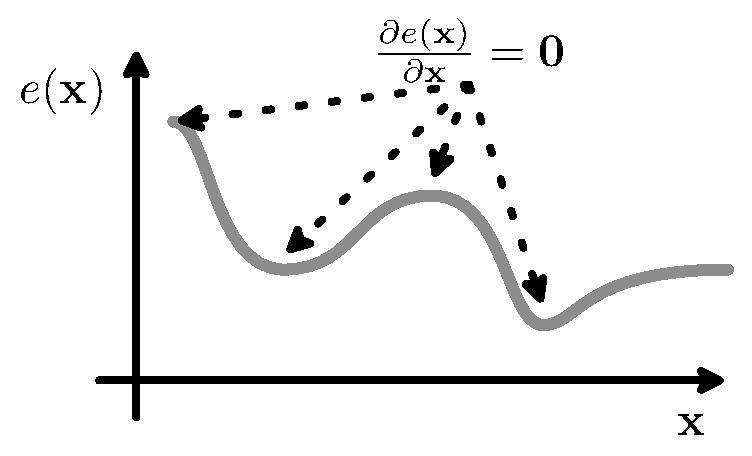
\includegraphics[width=0.8\textwidth]{chapters/minimization-fx/minimoex2.eps}
         \caption{$\VECTOR{b} \neq \VECTOR{f}(\VECTOR{x})$.}
         \label{fig:ex0b}
     \end{subfigure}
     \hfill
     \begin{subfigure}[b]{0.48\textwidth}
         \centering
         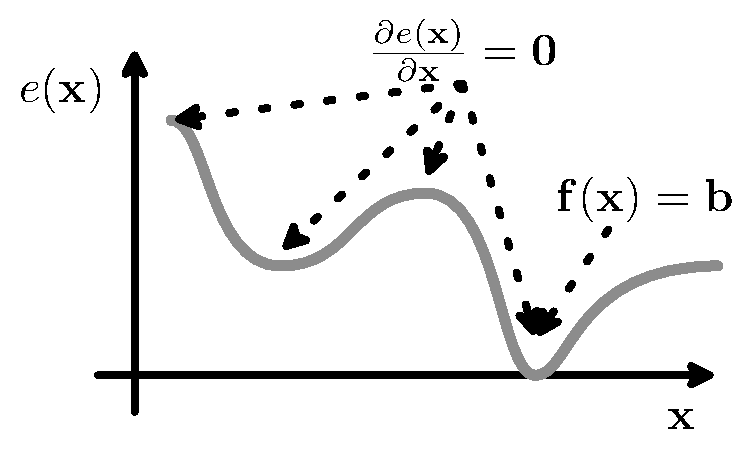
\includegraphics[width=0.8\textwidth]{chapters/minimization-fx/minimoex1.eps}
         \caption{$\VECTOR{b} = \VECTOR{f}(\VECTOR{x})$.}
         \label{fig:ex0a}
     \end{subfigure}
        \caption{Possibilidades para $\frac{\partial e(\VECTOR{x})}{\partial \VECTOR{x} }$.}
        \label{fig:ex0}
\end{figure}


Por outro lado, podemos realizar uma aproximação linear de $\VECTOR{f}(\VECTOR{x})$ em $e(\VECTOR{x})$
ao redor do ponto $\VECTOR{p}$ usando a \hyperref[def:taylor]{\textbf{série de Taylor}},
de modo que a Eq. (\ref{eq:proof:minfxbCfxb0}) pode ficar expresada como
\begin{equation}\label{eq:proof:minfxbCfxb0approx}
e(\VECTOR{x}) \approx ||\MATRIX{J}(\VECTOR{p})(\VECTOR{x}-\VECTOR{p})-(\VECTOR{b}-\VECTOR{f}(\VECTOR{p}))||_{\MATRIX{C}}^2,
\end{equation}
onde $\MATRIX{J}(\VECTOR{p})$ representa a \hyperref[def:jacobian]{\textbf{matriz Jacobiana}} 
de $\VECTOR{f}(\VECTOR{x})$ avaliada no ponto $\VECTOR{p}$.
Assim, usando o resultado da Prova \ref{proof:theo:minAxbCAxb} na Eq. (\ref{eq:proof:minfxbCfxb0approx}), 
podemos concluir que um ponto $\VECTOR{x}^*$ que é 
um mínimo da aproximação linear feita em $e(\VECTOR{x})$ ao redor do ponto $\VECTOR{p}$,
pode ser achado como
\begin{equation}\label{eq:proof:minAxbCAxb2approx}
\VECTOR{x}^* \approx \VECTOR{p}+ \left[ \MATRIX{J}(\VECTOR{p})^{\transpose}\MATRIX{C}\MATRIX{J}(\VECTOR{p}) \right]^{-1} \MATRIX{J}(\VECTOR{p})^{\transpose}\MATRIX{C} \left[\VECTOR{b}-\VECTOR{f}(\VECTOR{p})\right].
\end{equation}


Desta equação podemos tirar a seguintes conclusões:
\begin{itemize}

\item Observamos que a posição $\VECTOR{p}$ é corregida para ficar próximo à posição $\VECTOR{x}^*$, 
que é o valor mínimo na aproximação linear ao redor de $\VECTOR{p}$;
pelo que se deduz que a Eq. (\ref{eq:proof:minAxbCAxb2approx})
pode ser usada para procurar aproximações de pontos mínimos $\VECTOR{\hat{x}}$ em $e(\VECTOR{x})$ desde a posição $\VECTOR{p}$,
ou pelo menos aproximações de novas posições em caminhos numa direção descendente de $e(\VECTOR{x})$.

\item A Eq. (\ref{eq:proof:minAxbCAxb2approx}) é satisfeita 
com $\VECTOR{x}^* \approx \VECTOR{p}$ se acharmos um  
ponto $\VECTOR{p}$ onde  $\VECTOR{b} \approx \VECTOR{f}(\VECTOR{p})$; 
é dizer um mínimo global de $e(\VECTOR{x})$ em $\VECTOR{p}$, como pode ser visto na Figura \ref{fig:ex0a}. 

\item Se reescrevemos a Eq. (\ref{eq:proof:minAxbCAxb2approx}) usando o Teorema \ref{theo:derfxbCfxb0},
obtemos
\begin{equation}\label{eq:proof:minfxbCfxb2ea}
\VECTOR{x}^* \approx \VECTOR{p} -
0.5 \left[ \MATRIX{J}(\VECTOR{p})^{\transpose}\MATRIX{C} \MATRIX{J}(\VECTOR{p}) \right]^{-1}
\frac{\partial e(\VECTOR{p})}{\partial \VECTOR{x} },
\end{equation}
onde a Eq. (\ref{eq:proof:minfxbCfxb2ea}) é satisfeita 
com $\VECTOR{x}^* \approx \VECTOR{p}$
se acharmos um  ponto $\VECTOR{p}$ onde  
$\frac{\partial e(\VECTOR{p})}{\partial \VECTOR{x} }\approx \VECTOR{0}$; 
é dizer $\VECTOR{p}$ é um ponto de inflexão de $e(\VECTOR{x})$, como pode ser visto na Figura \ref{fig:ex0b}.
Porém, dado que a equação avança desde $\VECTOR{p}$ na direção de um mínimo $\VECTOR{x}^*$, 
mesmo que nos pontos de inflexão correspondentes a máximos ou pontos de sela,
encontremos valores de $\VECTOR{p}$ próximos a $\VECTOR{x}^*$,
 estes casos serão pouco estáveis pois
a correção da posição $\VECTOR{p}$ será na direção de um mínimo e não do máximo,
pois seguindo o Teorema \ref{theo:semipositivematrix1} a 
matriz $\MATRIX{J}(\VECTOR{p})^{\transpose}\MATRIX{C} \MATRIX{J}(\VECTOR{p})$ é 
semidefinida positiva se $\MATRIX{C}$ é simétrica.

\item Se modificamos a Eq. (\ref{eq:proof:minAxbCAxb2approx}), e escolhemos um ponto  
$\VECTOR{p}_0$ que consideremos próximo ao ponto $\VECTOR{\hat{x}}$ que minimiza $e(\VECTOR{\hat{x}})$,
podemos achar iterativamente aproximações lineares $\VECTOR{x}^*$ cada vez mais próximos a  $\VECTOR{\hat{x}}$,
se usamos a seguinte equação iterativa,
\begin{equation}\label{eq:proof:minfxbCfxb3}
\VECTOR{p}_{k} \leftarrow \VECTOR{p}_{k-1} -
\left[ \MATRIX{J}(\VECTOR{p}_{k-1})^{\transpose}\MATRIX{C} \MATRIX{J}(\VECTOR{p}_{k-1}) \right]^{-1}
\MATRIX{J}(\VECTOR{p}_{k-1})^{\transpose}\MATRIX{C} \left(\VECTOR{f}(\VECTOR{p}_{k-1})-\VECTOR{b}\right),
\end{equation}
iniciando desde um $\VECTOR{p}_{0}$, 
ate que exista uma tendência prolongada onde se observe que $\VECTOR{p}_{k}$ é muito próximo a $\VECTOR{p}_{k-1}$,
momento no qual declaramos que $\VECTOR{\hat{x}} \approx \VECTOR{p}_{k}$.
\item Como foi visto na Figura  \ref{fig:ex0b},
pode existir um mínimo global $\VECTOR{\hat{x}}$ de $e(\VECTOR{\hat{x}})>0$.
Isto nos restringe a que no uso da Eq. (\ref{eq:proof:minfxbCfxb3}),
nosso critério principal para estabelecer o final do cáculo iterativo,
deve ser a tendência na  proximidade entre $\VECTOR{p}_{k}$ e $\VECTOR{p}_{k-1}$ 
e não o valor de $e(\VECTOR{x}_k)$.
\end{itemize}~

Um diagrama completo resumindo todas estas conclusões pode ser visto na Figura \ref{fig:fluxo1}.
\end{myproofT}
\begin{figure}[!h]
     \centering
         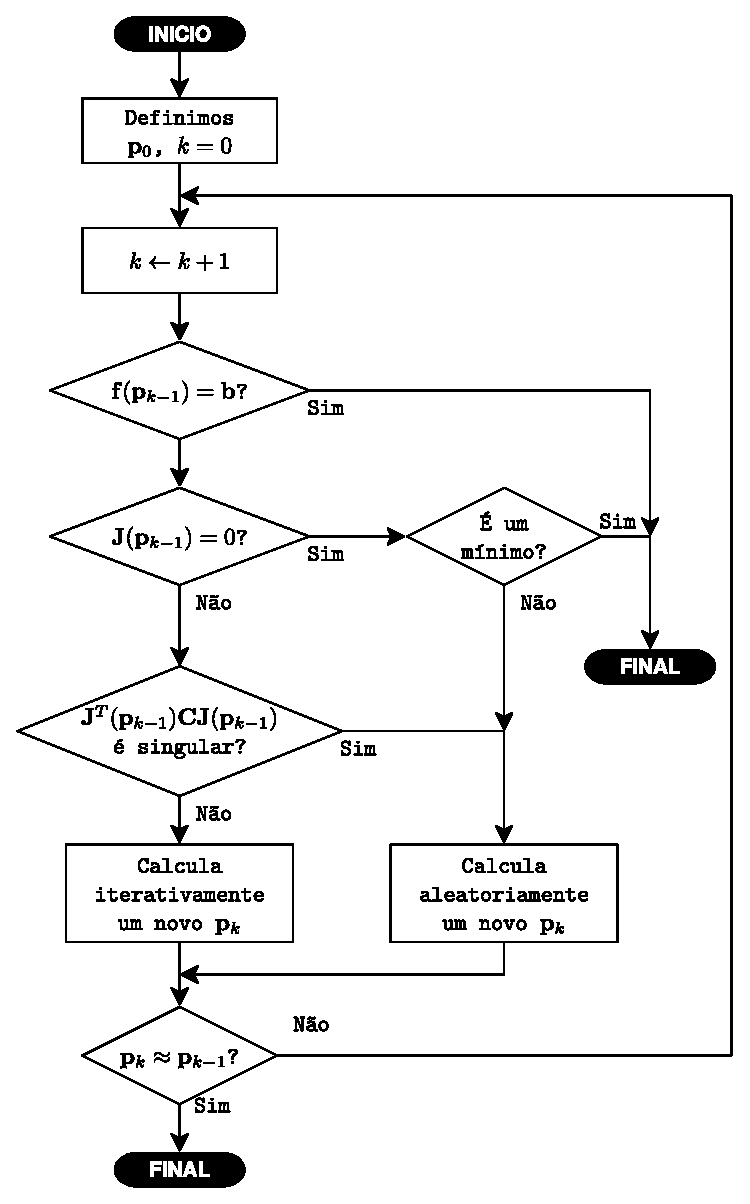
\includegraphics[width=0.75\textwidth]{chapters/minimization-fx/fluxo1.eps}
        \caption{Diagrama de fluxo da solução iterativa para achar um mínimo, seguindo a Prova \ref{proof:theo:minfxbCfxb}.}
        \label{fig:fluxo1}
\end{figure}


%%%%%%%%%%%%%%%%%%%%%%%%%%%%%%%%%%%%%%%%%%%%%%%%%%%%%%%%%%%%%%%%%%%%%%%%%%%%%%%%%%%%%%%
%%%%%%%%%%%%%%%%%%%%%%%%%%%%%%%%%%%%%%%%%%%%%%%%%%%%%%%%%%%%%%%%%%%%%%%%%%%%%%%%%%%%%%%
\begin{myproofT}[Relativa ao Teorema \ref{theo:minfxbCfxbaxqaxq}:]\label{proof:theo:minfxbCfxbaxqd}
Dados,
um escalar $\alpha\in \mathbb{R}_+$,
os vetores coluna $\VECTOR{x}\in \mathbb{R}^N$, 
$\VECTOR{q}\in \mathbb{R}^N$ e
$\VECTOR{b}\in \mathbb{R}^M$,  
uma função $\VECTOR{f}:\mathbb{R}^{N} \rightarrow \mathbb{R}^{M}$, 
as matrizes diagonais $\MATRIX{C} \in \mathbb{R}^{M\times M}_+$ e $\MATRIX{D} \in \mathbb{R}^{N\times N}_+$, e 
definida a Eq. (\ref{eq:proof:minfxbCfxbaxqd0}),
\begin{equation}\label{eq:proof:minfxbCfxbaxqd0}
e(\VECTOR{x})=||\VECTOR{f}(\VECTOR{x})-\VECTOR{b}||_{\MATRIX{C}}^2+\alpha||\VECTOR{x}-\VECTOR{q}||_{\MATRIX{D}}^2;
\end{equation}
sabemos que para achar o ponto $\VECTOR{x}=\VECTOR{\hat{x}}$ que gere o menor valor de $e(\VECTOR{x})$, é aplicado
o critério que um ponto de inflexão $\VECTOR{x}^+$; é dizer, um máximo, um mínimo ou um ponto de sela, pode ser achado quando 
$\frac{\partial e(\VECTOR{x}^+)}{\partial \VECTOR{x} }=[0~ 0~ \hdots~ 0 ]^{\transpose}$ (ver Figura \ref{fig:ex0b});
assim, usando o Teorema \ref{theo:derfxbCfxb0} e o Corolário \ref{coro:derAxbAxb2} obtemos que
\begin{equation}\label{eq:proof:minfxbCfxb1exact2}
2 \MATRIX{J}(\VECTOR{x}^+)^{\transpose}\MATRIX{C}\left[ \VECTOR{f}(\VECTOR{x}^+)-\VECTOR{b} \right] +
2 \alpha\MATRIX{D}\left[\VECTOR{x}^+-\VECTOR{q}\right]
=
\frac{\partial e(\VECTOR{x}^+)}{\partial \VECTOR{x} }=[0~ 0~ \hdots~ 0 ]^{\transpose},
\end{equation}
Da Eq. (\ref{eq:proof:minfxbCfxb1exact2}) observamos, 
que podemos achar um ponto de inflexão $\VECTOR{q}$
em $e(\VECTOR{q})$ se 
$\MATRIX{J}(\VECTOR{q})  = \MATRIX{0}$ ou um mínimo geral se $\VECTOR{f}(\VECTOR{q})=\VECTOR{b}$,
caso contrario, 
se nenhuma destas possibilidades são cumpridas devemos aplicar outros critérios para achar os pontos de inflexão.

Assim, procurando outros critérios, podemos realizar uma aproximação linear de $\VECTOR{f}(\VECTOR{x})$ em $e(\VECTOR{x})$
ao redor do ponto $\VECTOR{p}$ usando a \hyperref[def:taylor]{\textbf{série de Taylor}},
de modo que a Eq. (\ref{eq:proof:minfxbCfxbaxqd0}) pode ficar expressada como
\begin{equation}\label{eq:proof:minfxbCfxb0alphaxqDapprox}
e(\VECTOR{x}) \approx 
||\MATRIX{J}(\VECTOR{p})[\VECTOR{x}-\VECTOR{p}]-[\VECTOR{b}-\VECTOR{f}(\VECTOR{p})]||_{\MATRIX{C}}^2+
\alpha||[\VECTOR{x}-\VECTOR{p}]-[\VECTOR{q}-\VECTOR{p}]||_{\MATRIX{D}}^2,
\end{equation}
onde $\MATRIX{J}(\VECTOR{p})$ representa a \hyperref[def:jacobian]{\textbf{matriz Jacobiana}} 
de $\VECTOR{f}(\VECTOR{x})$ avaliada no ponto $\VECTOR{p}$.
Assim, usando o resultado da Prova \ref{proof:theo:minAxbCAxbalphaxqD} na Eq. (\ref{eq:proof:minfxbCfxb0alphaxqDapprox}), 
podemos concluir que um ponto $\VECTOR{x}^*$ que é 
um mínimo da aproximação linear feita em $e(\VECTOR{x})$ ao redor do ponto $\VECTOR{p}$,
pode ser achado como
\begin{equation}\label{eq:proof:minfxbCfxbaxqd2}
\VECTOR{x}^* \approx \VECTOR{p} +
\left[ \MATRIX{J}(\VECTOR{p})^{\transpose}\MATRIX{C} \MATRIX{J}(\VECTOR{p})+\alpha \MATRIX{D} \right]^{-1}
\left\{ \MATRIX{J}(\VECTOR{p})^{\transpose}\MATRIX{C} \left[\VECTOR{b}-\VECTOR{f}(\VECTOR{p})\right]-\alpha\MATRIX{D}[\VECTOR{p}-\VECTOR{q}]\right\}.
\end{equation}


Desta equação podemos tirar a seguintes conclusões:
\begin{itemize}

\item Observamos que a posição $\VECTOR{p}$ é corregida para ficar próximo à posição $\VECTOR{x}^*$, 
que é o valor mínimo na aproximação linear ao redor de $\VECTOR{p}$;
pelo que se deduz que a Eq. (\ref{eq:proof:minfxbCfxbaxqd2})
pode ser usada para procurar aproximações de pontos mínimos $\VECTOR{\hat{x}}$ em $e(\VECTOR{x})$ desde a posição $\VECTOR{p}$,
ou pelo menos aproximações de novas posições em caminhos numa direção descendente 
de $e(\VECTOR{x})$ desde a posição $\VECTOR{p}$.

\begin{comment}
\item A Eq. (\ref{eq:proof:minfxbCfxbaxqd2}) é satisfeita 
com $\VECTOR{x}^* \approx \VECTOR{p}$ se acharmos um  
ponto $\VECTOR{p}$ onde  $\VECTOR{b} \approx \VECTOR{f}(\VECTOR{p}\approx \VECTOR{q})$; 
é dizer um mínimo global de $e(\VECTOR{x})$ em $\VECTOR{p}$, como pode ser visto na Figura \ref{fig:ex0a}. 
\end{comment}

\item Se reescrevemos a Eq. (\ref{eq:proof:minfxbCfxbaxqd2}) usando o Teorema \ref{theo:derfxbCfxb0}
e o Corolário \ref{coro:derAxbAxb2},
obtemos
\begin{equation}\label{eq:proof:minfxbCfxb2ea1}
\VECTOR{x}^* \approx \VECTOR{p} -
0.5 \left[ \MATRIX{J}(\VECTOR{p})^{\transpose}\MATRIX{C} \MATRIX{J}(\VECTOR{p})+\alpha \MATRIX{D} \right]^{-1}
\frac{\partial e(\VECTOR{p})}{\partial \VECTOR{x} },
\end{equation}
onde a Eq. (\ref{eq:proof:minfxbCfxb2ea1}) é satisfeita 
com $\VECTOR{x}^* \approx \VECTOR{p}$
se acharmos um  ponto $\VECTOR{p}$ onde  
$\frac{\partial e(\VECTOR{p})}{\partial \VECTOR{x} }\approx \VECTOR{0}$,
 como descrito na Eq. (\ref{eq:proof:minfxbCfxb1exact2}); 
é dizer $\VECTOR{p}$ é um ponto de inflexão de $e(\VECTOR{x})$, ver Figura \ref{fig:ex0b}.
Porém, dado que a equação avança desde $\VECTOR{p}$ na direção de um mínimo $\VECTOR{x}^*$, 
mesmo que nos pontos de inflexão correspondentes a máximos ou pontos de sela,
encontremos valores de $\VECTOR{p}$ próximos a $\VECTOR{x}^*$,
 estes casos serão pouco estáveis pois
a correção da posição $\VECTOR{p}$ será na direção de um mínimo e não do máximo,
pois seguindo o Teorema \ref{theo:semipositivematrix1}, se $\MATRIX{C}$ e $\MATRIX{D}$ são simétricas, 
então as matrizes $\MATRIX{J}(\VECTOR{p})^{\transpose}\MATRIX{C} \MATRIX{J}(\VECTOR{p})$ e $\MATRIX{D}$
são semidefinidas positivas.

\item Se modificamos a Eq. (\ref{eq:proof:minfxbCfxbaxqd2}), e escolhemos um ponto  
$\VECTOR{p}_0$ que consideremos próximo ao ponto $\VECTOR{x}=\VECTOR{\hat{x}}$ que minimiza $e(\VECTOR{x})$,
podemos achar iterativamente aproximações lineares $\VECTOR{x}^*$ cada vez mais próximos a  $\VECTOR{\hat{x}}$,
se usamos a seguinte equação iterativa,
\begin{equation}\label{eq:proof:minfxbCfxb3a}
\VECTOR{p}_{k} \leftarrow \VECTOR{p}_{k-1} -
\left[ \MATRIX{J}(\VECTOR{p}_{k-1})^{\transpose}\MATRIX{C} \MATRIX{J}(\VECTOR{p}_{k-1}) +\alpha \MATRIX{D}\right]^{-1}
\left\{ \MATRIX{J}(\VECTOR{p}_{k-1})^{\transpose}\MATRIX{C} \left[\VECTOR{f}(\VECTOR{p}_{k-1})-\VECTOR{b}\right]+
\alpha\MATRIX{D}[\VECTOR{p}_{k-1}-\VECTOR{q}]\right\},
\end{equation}
iniciando desde um $\VECTOR{p}_{0}$ 
ate que exista uma tendência prolongada onde se observe que $\VECTOR{p}_{k}$ é muito próximo a $\VECTOR{p}_{k-1}$,
momento no qual declaramos que $\VECTOR{\hat{x}} \approx \VECTOR{p}_{k}$.
\item Como foi visto na Figura  \ref{fig:ex0b},
pode existir um mínimo global $\VECTOR{x}=\VECTOR{\hat{x}}$ de $e(\VECTOR{x}) > 0$.
Isto nos restringe a que no uso da Eq. (\ref{eq:proof:minfxbCfxb3a}),
nosso critério principal para estabelecer o final do cáculo iterativo,
deve ser a tendência na  proximidade entre $\VECTOR{p}_{k}$ e $\VECTOR{p}_{k-1}$ 
e não o valor de $e(\VECTOR{x}_k)$.
\end{itemize}

Um diagrama completo resumindo todas estas conclusões pode ser visto na Figura \ref{fig:fluxo2}.
\end{myproofT}
\begin{figure}[!h]
     \centering
         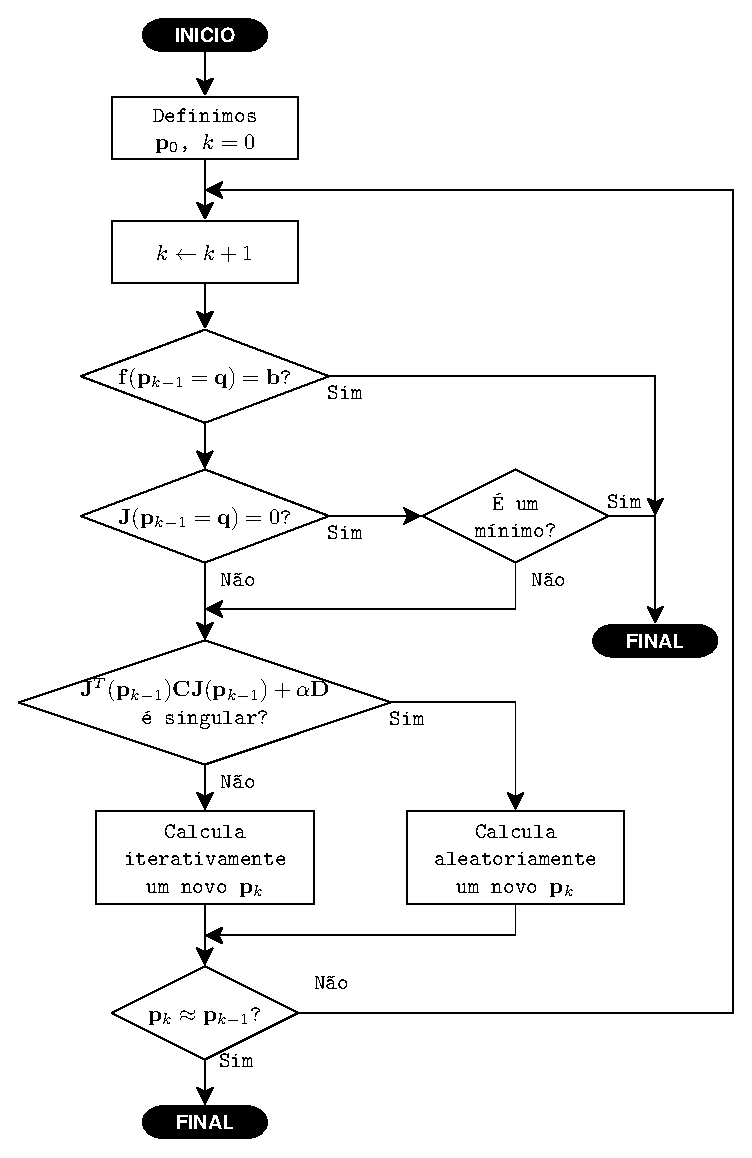
\includegraphics[width=0.75\textwidth]{chapters/minimization-fx/fluxo2.eps}
        \caption{Diagrama de fluxo da solução iterativa para achar um mínimo, seguindo a Prova \ref{proof:theo:minfxbCfxbaxqd}.}
        \label{fig:fluxo2}
\end{figure}

%%%%%%%%%%%%%%%%%%%%%%%%%%%%%%%%%%%%%%%%%%%%%%%%%%%%%%%%%%%%%%%%%%%%%%%%%%%%%%%%%%%%%%%
%%%%%%%%%%%%%%%%%%%%%%%%%%%%%%%%%%%%%%%%%%%%%%%%%%%%%%%%%%%%%%%%%%%%%%%%%%%%%%%%%%%%%%%
\begin{myproofT}[Relativa ao Teorema \ref{theo:minfxbCfxbaxoaxo}:]\label{proof:theo:minfxbCfxbaxod}
Dados,
um escalar $\alpha\in \mathbb{R}_+$,
os vetores coluna $\VECTOR{x}\in \mathbb{R}^N$, 
$\VECTOR{x}_{last}\in \mathbb{R}^N$ e
$\VECTOR{b}\in \mathbb{R}^M$,  
uma função $\VECTOR{f}:\mathbb{R}^{N} \rightarrow \mathbb{R}^{M}$, 
as matrizes diagonais $\MATRIX{C} \in \mathbb{R}^{M\times M}$ e $\MATRIX{D} \in \mathbb{R}^{N\times N}$, e 
definida a Eq. (\ref{eq:proof:minfxbCfxbaxod0}),
\begin{equation}\label{eq:proof:minfxbCfxbaxod0}
e(\VECTOR{x})=||\VECTOR{f}(\VECTOR{x})-\VECTOR{b}||_{\MATRIX{C}}^2+\alpha||\VECTOR{x}-\VECTOR{x}_{last}||_{\MATRIX{D}}^2,
\end{equation}
tendo em consideração que $\VECTOR{x}_{last}$ é uma constante equivalente a $\VECTOR{x}_{k-1}$
numa busca iterativa ou equivalente a $\VECTOR{p}$, 
se decidimos usar uma aproximação linear ao redor de $\VECTOR{p}$ em $\VECTOR{f}(\VECTOR{x})$; 
é dizer, o segundo somando na Eq. (\ref{eq:proof:minfxbCfxbaxod0}) 
procura minimizar $||\VECTOR{x}_{k}-\VECTOR{x}_{k-1}||_{\MATRIX{D}}^2$.

Sabemos que para achar o ponto $\VECTOR{x}=\VECTOR{\hat{x}}$ que gere o menor valor de $e(\VECTOR{x})$, é aplicado
o critério que um ponto de inflexão $\VECTOR{x}^+$; é dizer, um máximo, um mínimo ou um ponto de sela, pode ser achado quando 
$\frac{\partial e(\VECTOR{x}^+)}{\partial \VECTOR{x} }=[0~ 0~ \hdots~ 0 ]^{\transpose}$ (ver Figura \ref{fig:ex0b});
assim, usando o Teorema \ref{theo:derfxbCfxb0} e o Corolário \ref{coro:derAxbAxb2} obtemos que
\begin{equation}\label{eq:proof:minfxbCfxbaxod1exact2}
2 \MATRIX{J}(\VECTOR{x}^+)^{\transpose}\MATRIX{C}\left[ \VECTOR{f}(\VECTOR{x}^+)-\VECTOR{b} \right] +
2 \alpha\MATRIX{D}\left[\VECTOR{x}^+-\VECTOR{x}_{last}\right]
=
\frac{\partial e(\VECTOR{x}^+)}{\partial \VECTOR{x} }=[0~ 0~ \hdots~ 0 ]^{\transpose}.
\end{equation}
Da Eq. (\ref{eq:proof:minfxbCfxbaxod1exact2}) observamos, 
que podemos achar um ponto de inflexão $\VECTOR{x}^+=\VECTOR{x}_{last}$
em $e(\VECTOR{x}_{last})$ se 
$\MATRIX{J}(\VECTOR{x}_{last})  = \MATRIX{0}$ ou um mínimo geral se $\VECTOR{f}(\VECTOR{x}_{last})=\VECTOR{b}$,
caso contrario, 
se nenhuma destas possibilidades são cumpridas devemos aplicar outros critérios para achar os pontos de inflexão.



Assim, procurando outros critérios, podemos igualar $\VECTOR{x}_{last}\equiv \VECTOR{p}$ e 
realizar uma aproximação linear de $\VECTOR{f}(\VECTOR{x})$ em $e(\VECTOR{x})$
ao redor do ponto $\VECTOR{p}$ usando a \hyperref[def:taylor]{\textbf{série de Taylor}} truncada,
de modo que a Eq. (\ref{eq:proof:minfxbCfxbaxod0}) pode ficar expressada como
\begin{equation}\label{eq:proof:minfxbCfxbaxod0alphaxqDapprox}
e(\VECTOR{x}) \approx e_{\VECTOR{p}}(\VECTOR{x})  \equiv 
||\MATRIX{J}(\VECTOR{p})[\VECTOR{x}-\VECTOR{p}]-[\VECTOR{b}-\VECTOR{f}(\VECTOR{p})]||_{\MATRIX{C}}^2+
\alpha||\VECTOR{x}-\VECTOR{p}||_{\MATRIX{D}}^2,
\end{equation}
onde $\MATRIX{J}(\VECTOR{p})$ representa a \hyperref[def:jacobian]{\textbf{matriz Jacobiana}} 
de $\VECTOR{f}(\VECTOR{x})$ avaliada no ponto $\VECTOR{p}$.
Assim, usando o resultado da Prova \ref{proof:theo:minAxbCAxbalphaxqD} na Eq. (\ref{eq:proof:minfxbCfxbaxod0alphaxqDapprox}), 
onde se aplica que $\frac{\partial e_{\VECTOR{p}}(\VECTOR{x}^*)}{\partial \VECTOR{x} }=\VECTOR{0}$,
podemos concluir que um ponto $\VECTOR{x}^*$ que é 
um mínimo da aproximação linear feita em $e(\VECTOR{x})$ ao redor do ponto $\VECTOR{p}$,
pode ser achado como,
\begin{equation}\label{eq:proof:minfxbCfxbaxod2}
\VECTOR{x}^* \approx \VECTOR{p} +
\left[ \MATRIX{J}(\VECTOR{p})^{\transpose}\MATRIX{C} \MATRIX{J}(\VECTOR{p})+\alpha \MATRIX{D} \right]^{-1}
\MATRIX{J}(\VECTOR{p})^{\transpose}\MATRIX{C} \left[\VECTOR{b}-\VECTOR{f}(\VECTOR{p})\right].
\end{equation}

Desta equação podemos tirar a seguintes conclusões:
\begin{itemize}

\item Observamos que a posição $\VECTOR{p}$ é corregida para ficar próximo à posição $\VECTOR{x}^*$, 
que é o valor mínimo na aproximação linear ao redor de $\VECTOR{p}$;
pelo que se deduz que a Eq. (\ref{eq:proof:minfxbCfxbaxod2})
pode ser usada para procurar aproximações de pontos mínimos $\VECTOR{\hat{x}}$ em $e(\VECTOR{x})$ desde a posição $\VECTOR{p}$,
ou pelo menos aproximações de novas posições em caminhos numa direção descendente de $e(\VECTOR{x})$.

\item A Eq. (\ref{eq:proof:minfxbCfxbaxod2}) é satisfeita 
com $\VECTOR{x}^* \approx \VECTOR{p}$ se acharmos um  
ponto $\VECTOR{p}$ onde  $\VECTOR{b} \approx \VECTOR{f}(\VECTOR{p}\approx \VECTOR{x}_{last})$; 
é dizer um mínimo global de $e(\VECTOR{x})$ em $\VECTOR{p}$, como pode ser visto na Figura \ref{fig:ex0a}. 

\item Se reescrevemos a Eq. (\ref{eq:proof:minfxbCfxbaxod2}) usando o Teorema \ref{theo:derfxbCfxb0}
e o Corolário \ref{coro:derAxbAxb2},
obtemos
\begin{equation}\label{eq:proof:minfxbCfxbaxod2ea1}
\VECTOR{x}^* \approx \VECTOR{p} -
0.5 \left[ \MATRIX{J}(\VECTOR{p})^{\transpose}\MATRIX{C} \MATRIX{J}(\VECTOR{p})+\alpha \MATRIX{D} \right]^{-1}
\frac{\partial e(\VECTOR{p})}{\partial \VECTOR{x} },
\end{equation}
onde a Eq. (\ref{eq:proof:minfxbCfxbaxod2ea1}) é satisfeita 
com $\VECTOR{x}^* \approx \VECTOR{p}$
se acharmos um  ponto $\VECTOR{p}$ onde  
$\frac{\partial e(\VECTOR{p})}{\partial \VECTOR{x} }\approx \VECTOR{0}$; 
é dizer $\VECTOR{p}$ é um ponto de inflexão de $e(\VECTOR{x})$, como pode ser visto na Figura \ref{fig:ex0b}.
Porém, dado que a equação avança desde $\VECTOR{p}$ na direção de um mínimo $\VECTOR{x}^*$, 
mesmo que nos pontos de inflexão correspondentes a máximos ou pontos de sela,
encontremos valores de $\VECTOR{p}$ próximos a $\VECTOR{x}^*$,
 estes casos serão pouco estáveis pois
a correção da posição $\VECTOR{p}$ será na direção de um mínimo e não do máximo.
\item Seguindo o Teorema \ref{theo:semipositivematrix1}, se $\MATRIX{C}$ e $\MATRIX{D}$ são simétricas, 
então as matrizes $\MATRIX{J}(\VECTOR{p})^{\transpose}\MATRIX{C} \MATRIX{J}(\VECTOR{p})$ e $\MATRIX{D}$
são semidefinidas positivas.

\item Se modificamos a Eq. (\ref{eq:proof:minfxbCfxbaxod2}), e escolhemos um ponto  
$\VECTOR{p}_0$ que consideremos próximo ao ponto $\VECTOR{x}=\VECTOR{\hat{x}}$ que minimiza $e(\VECTOR{x})$,
podemos achar iterativamente aproximações lineares $\VECTOR{x}^*$ cada vez mais próximos a  $\VECTOR{\hat{x}}$,
se usamos a seguinte equação iterativa,
\begin{equation}\label{eq:proof:minfxbCfxbaxod3b}
\VECTOR{p}_{k} \leftarrow \VECTOR{p}_{k-1} -
\left[ \MATRIX{J}(\VECTOR{p}_{k-1})^{\transpose}\MATRIX{C} \MATRIX{J}(\VECTOR{p}_{k-1}) +\alpha \MATRIX{D}\right]^{-1}
\MATRIX{J}(\VECTOR{p}_{k-1})^{\transpose}\MATRIX{C} \left[\VECTOR{f}(\VECTOR{p}_{k-1})-\VECTOR{b}\right],
\end{equation}
onde se inicia desde um $\VECTOR{p}_{0}$ 
ate que exista uma tendência prolongada onde se observe que $\VECTOR{p}_{k}$ é muito próximo a $\VECTOR{p}_{k-1}$,
momento no qual declaramos que $\VECTOR{\hat{x}} \approx \VECTOR{p}_{k}$.
Disto também se deduz que o erro a minimizar em cada iteração será diferente e influenciado pelo valor do ponto $\VECTOR{p}_{k-1}$,
\begin{equation}
e_{k-1}(\VECTOR{x})  \equiv 
||\VECTOR{f}(\VECTOR{x})-\VECTOR{b}||_{\MATRIX{C}}^2+
\alpha||\VECTOR{x}-\VECTOR{p}_{k-1}||_{\MATRIX{D}}^2
\end{equation}
\item Como foi visto na Figura  \ref{fig:ex0b},
pode existir um mínimo global $\VECTOR{x}=\VECTOR{\hat{x}}$ de $e(\VECTOR{x}) > 0$.
Isto nos restringe a que no uso da Eq. (\ref{eq:proof:minfxbCfxb3a}),
nosso critério principal para estabelecer o final do cálculo iterativo,
deve ser a tendência na  proximidade entre $\VECTOR{p}_{k}$ e $\VECTOR{p}_{k-1}$ 
e não o valor de $e(\VECTOR{x}_k)$.
\end{itemize}~

Um diagrama completo resumindo todas estas conclusões pode ser visto na Figura \ref{fig:fluxo3}.
\end{myproofT}
\begin{figure}[!h]
     \centering
         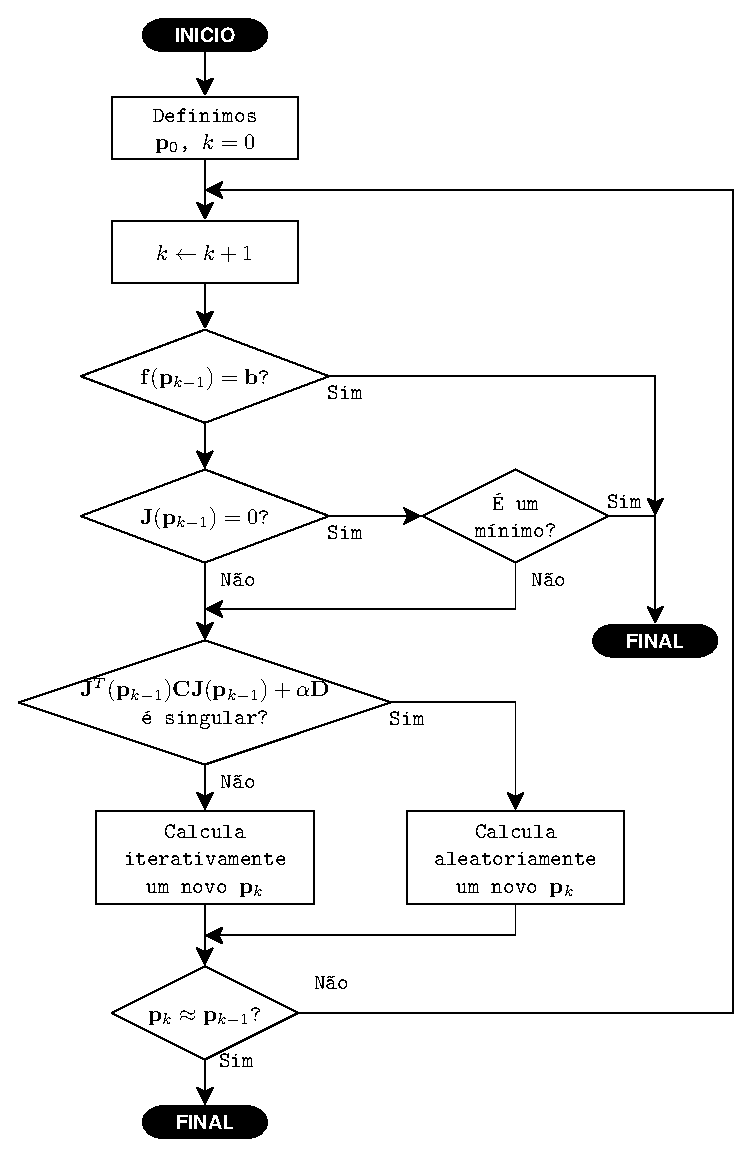
\includegraphics[width=0.75\textwidth]{chapters/minimization-fx/fluxo3.eps}
        \caption{Diagrama de fluxo da solução iterativa para achar um mínimo, seguindo a Prova \ref{proof:theo:minfxbCfxbaxod}.}
        \label{fig:fluxo3}
\end{figure}



%----------------------------------------------------------------------------------------
%	CHAPTER  
%----------------------------------------------------------------------------------------
\chapterimage{chapter_minimization2.pdf} % Chapter heading image

\chapter{Minimização do erro em funções: $\mathbb{R}$ $\rightarrow$ $\mathbb{R}$}

%%%%%%%%%%%%%%%%%%%%%%%%%%%%%%%%%%%%%%%%%%%%%%%%%%%%%%%%%%%%%%%%%%%%%%%%%%%%%%%%%%%%%%%
%%%%%%%%%%%%%%%%%%%%%%%%%%%%%%%%%%%%%%%%%%%%%%%%%%%%%%%%%%%%%%%%%%%%%%%%%%%%%%%%%%%%%%%
%%%%%%%%%%%%%%%%%%%%%%%%%%%%%%%%%%%%%%%%%%%%%%%%%%%%%%%%%%%%%%%%%%%%%%%%%%%%%%%%%%%%%%%
\section{Minimização de $||h(x)-a||^2$} 



\index{Minimização, métodos!Método de Newton}
%\index{Problema inverso!Não linear}
\index{Minimização do erro quadrático!Não linear}%!Função $||h(x)-a||^2$}

\begin{theorem}[Solução iterativa]\label{theo:minhxhx}
Dados,
um escalar $x \in \mathbb{R}$, 
um escalar $a \in \mathbb{R}$,  
uma função $h:\mathbb{R} \rightarrow \mathbb{R}$, e 
definida a Eq. (\ref{eq:minhxhx1}),
\begin{equation}\label{eq:minhxhx1}
e(x)=||h(x)-a||^2.
\end{equation}

Se desejamos ter o valor $\hat{x}$ que minimiza o escalar $e(\hat{x})$,
este valor pode ser achado\footnote{A 
demostração da Eq. (\ref{eq:minhxhx2}) pode ser vista na Prova \ref{proof:theo:minhxhx}.} 
usando iterativamente a Eq. (\ref{eq:minhxhx2}),
onde  $h'(x)\equiv \frac{d h(x)}{d x}$.
\begin{equation}\label{eq:minhxhx2}
x_{k} \leftarrow x_{k-1}-
\frac{ h(x_{k-1})-a}{h'(x_{k-1})},
\end{equation}


Assim, $\hat{x}$ pode ser achado iniciando a Eq. (\ref{eq:minhxhx2}) desde um 
$x_{0}$ qualquer, realizando cálculos $x_{k}$ iterativamente, 
ate que $x_{k}$ seja muito próximo a $x_{k-1}$ (convergência de $x_{k}$),
onde pode ser declarado que $\hat{x} \approx x_{k}$.

\textbf{Considerações:}
\begin{itemize} 
\item Para que tenha sentido a Eq. (\ref{eq:minhxhx2}),
 e consequentemente esta possa ser usada, devemos verificar que  $h'(x_{k-1})\neq 0$,
pois se $h'(x_{k-1})= 0$ indica que existe um ponto de inflexão 
(máximo, mínimo ou ponto de sela) em $e(x)$.
\item A busca iterativa da Eq. (\ref{eq:minhxhx2}) pode falhar se coincide que o mínimo $\hat{x}$ procurado
tem um $h'(x_{k-1})= 0$.
Este erro só acontece quando $x_{k-1}$ atinge de forma exata $\hat{x}$,
para valores próximos a $\hat{x}$ a busca iterativa de $x_{k}$ avança eficazmente.
\end{itemize}
\end{theorem}


\begin{tcbattention}
\begin{itemize}
\item Uma forma de iterar, como a vista na Eq. (\ref{eq:minhxhx2}) é conhecida como método de Newton.
\end{itemize}
\end{tcbattention}


%%%%%%%%%%%%%%%%%%%%%%%%%%%%%%%%%%%%%%%%%%%%%%%%%%%%%%%%%%%%%%%%%%%%%%%%%%%%%%%%
\subsection{Exemplos de minimização de $||h(x)-a||^2$}


\begin{example}\label{ex:minhxhx1}
Conhecida uma função $h(x)=x^2$ é valor $a=1$ do contradomínio de $h(x)$,
achar o valor $\hat{x}$ que minimize $e(x)=(h(x)-a)^2$.
\end{example}
\begin{SolutionT}[Relativa ao Exemplo \ref{ex:minhxhx1}:]\label{sol:minhxhx1}
 A Fig. \ref{fig:hxacasesa} nos mostra o processo de busca de um mínimo de $e(x)$. 
A busca inicia em $x_0=-1.5$, 
todos os valores $x_{k}$ podem ser vistos na
Tabela \ref{tab:hxacases1}. 
Neste caso a busca iterativa indicada pela Eq. (\ref{eq:minhxhx2}) converge sem problemas em $\hat{x}\approx x_4=-1$ com $e(\hat{x})\approx 0$.
%No caminho não foi achado nenhum ponto $x_{k}$ com $h'(x_{k})\cong 0$.
\end{SolutionT}

\begin{figure}[!h]
    \centering
    \begin{subfigure}[b]{0.49\textwidth}
        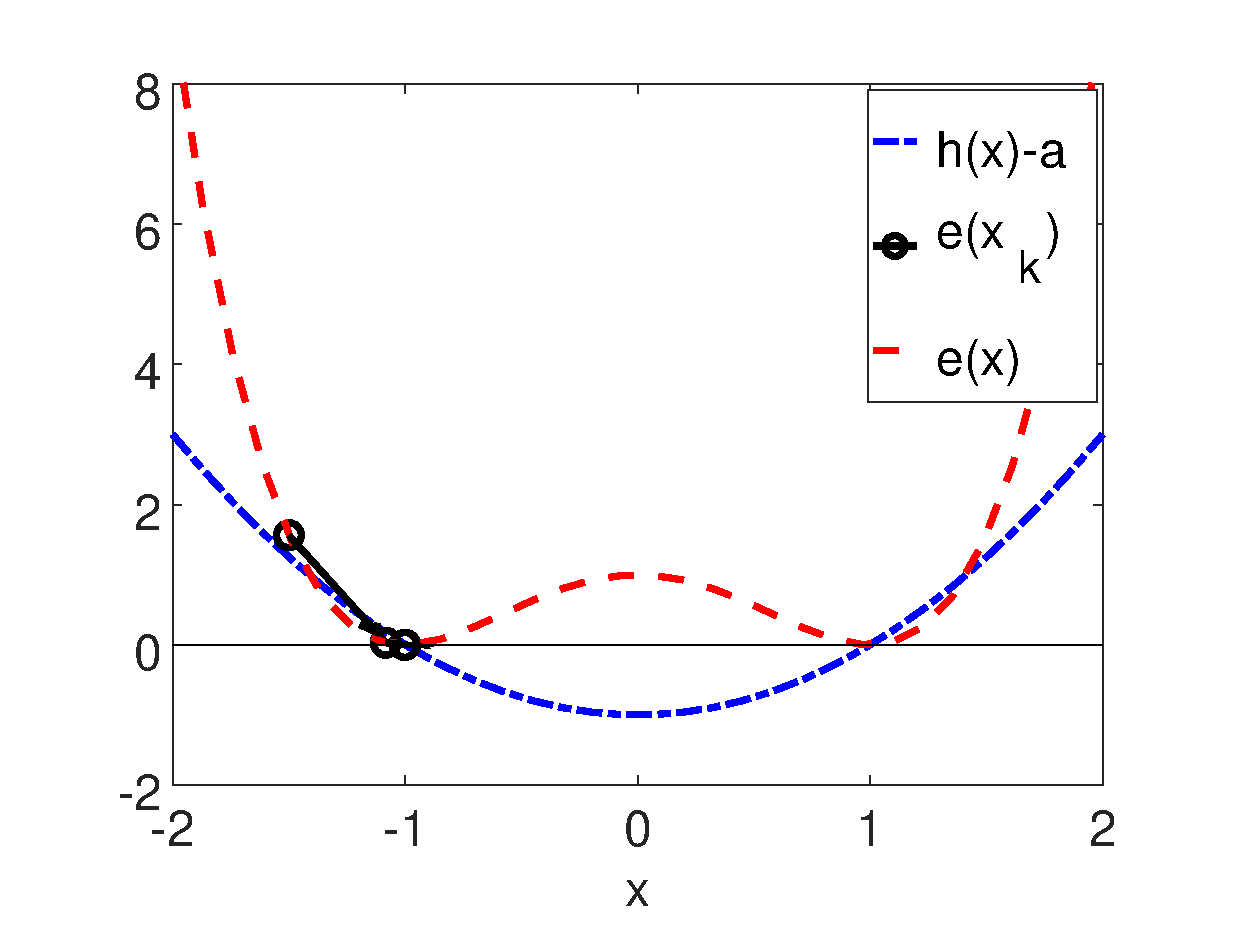
\includegraphics[width=\textwidth]{chapters/minimization-hx/mfiles/hx_a/minimizando_hx_a_1.eps}
        \caption{Usando $h(x)=x^2$ e $a=1$, quando as iterações convergem}
        \label{fig:hxacasesa}
    \end{subfigure}
    ~ %add desired spacing between images, e. g. ~, \quad, \qquad, \hfill etc. 
      %(or a blank line to force the subfigure onto a new line)
    \begin{subfigure}[b]{0.49\textwidth}
        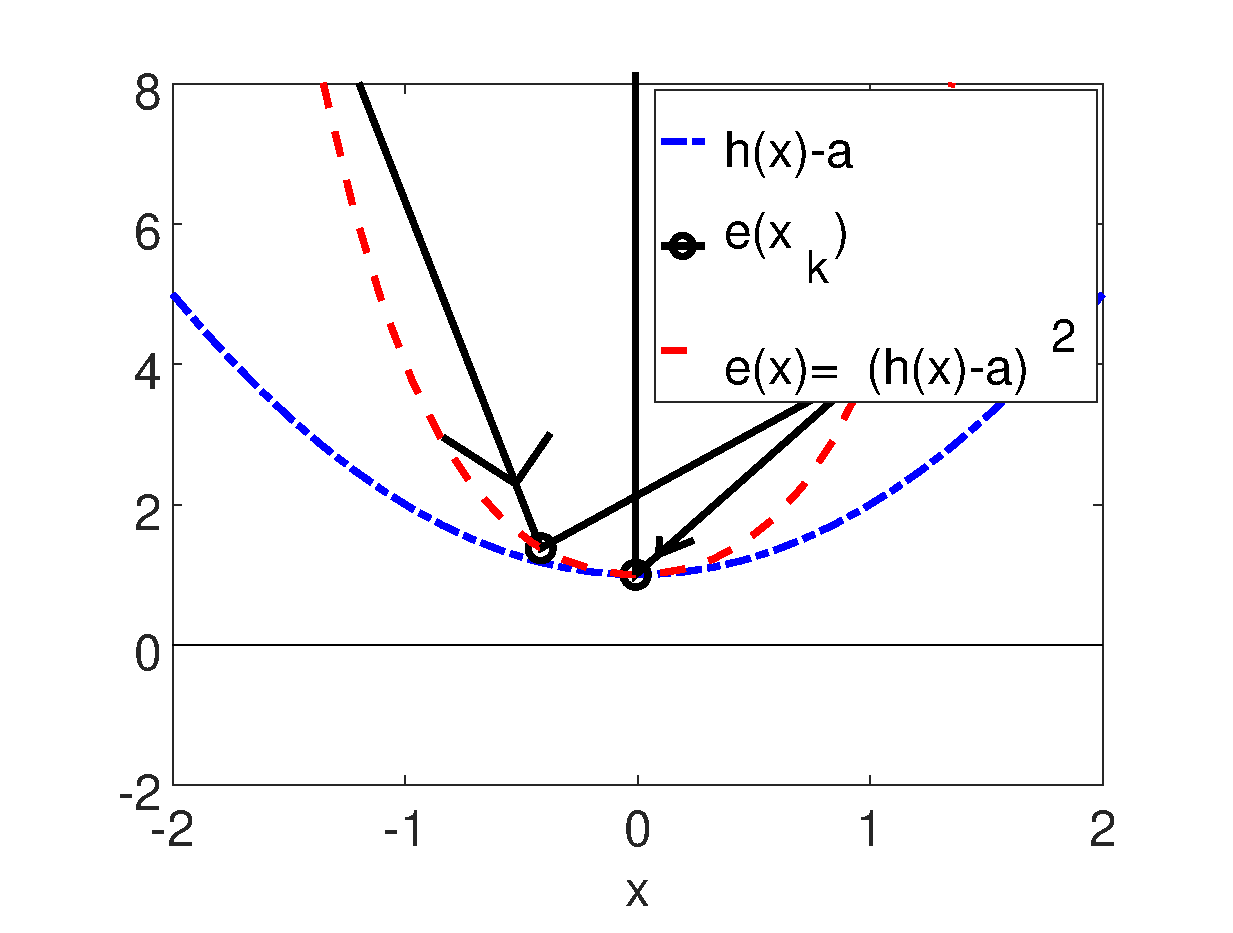
\includegraphics[width=\textwidth]{chapters/minimization-hx/mfiles/hx_a/minimizando_hx_a_2.eps}
        \caption{Usando $h(x)=x^2$ e $a=-1$, quando as iterações divergem}
        \label{fig:hxacasesb}
    \end{subfigure}
    \caption{Comportamento para $h(x)=x^2$ da equação iterativa do Teorema \ref{theo:minhxhx}}
    \label{fig:hxacases}
\end{figure}

\begin{table}[!h]
\centering
\begin{tabular}{|l|l|l|l|l|l|}
\hline
$k$      & 0 & 1 & 2 & 3 & 4 \\ \hline
$x_k$    & -1.5000 & -1.0833 & -1.0032 & -1.0000 & -1.0000 \\ \hline
$e(x_k)$ & 1.5625 & 3.0141e-02 & 4.1223e-05 & 1.0486e-10 & 6.8718e-22 \\ \hline
\end{tabular}
\caption{Resposta iterativa do Exemplo \ref{ex:minhxhx1}.}
\label{tab:hxacases1}
\end{table}

\begin{example}\label{ex:minhxhx2}
Conhecida uma função $h(x)=x^2$ é valor $a=-1$ do contradomínio de $h(x)$,
achar o valor $\hat{x}$ que minimize $e(x)=(h(x)-a)^2$.
\end{example}


\begin{SolutionT}[Relativa ao Exemplo \ref{ex:minhxhx2}:]\label{sol:minhxhx2}
A Fig. \ref{fig:hxacasesb} nos mostra o processo de busca de um mínimo de $e(x)$. 
A busca inicia em $x_0=-1.5$,
 todos os valores $x_{k}$ podem ser vistos na Tabela \ref{tab:hxacases2}. 
Neste caso a busca iterativa indicada pela Eq. (\ref{eq:minhxhx2}) diverge 
em $x_3\approx 0$ com $e(x_3)=1.0001$ que é o mínimo;
ao principio os valores de $x_{k}$ tendem a procurar o mínimo; porém,
perto de este valor se cumpre que $h'(x_{k})\cong 0$, e o valor de $x_{k}$ diverge
a um valor muito longe do mínimo; é fácil de observar, que neste caso se produz 
uma especie de efeito sanfona, onde $x_{k}$ se aproxima ao mínimo $e(x)$, e quando 
está muito próximo do mínimo o valor volta divergir.
\end{SolutionT}

\begin{table}[!h]
\centering
\begin{tabular}{|l|l|l|l|l|l|}
\hline
$k$      & 0 & 1 & 2 & 3 & 4 \\ \hline
$x_k$    & -1.5000 & -4.1667e-01 & 9.9167e-01 & -8.3683e-03 & 59.745 \\ \hline
$e(x_k)$ & 10.562 & 1.3774 & 3.9339 & 1.0001 & 1.2748e+07 \\ \hline
\end{tabular}
\caption{Resposta iterativa do Exemplo \ref{ex:minhxhx2}.}
\label{tab:hxacases2}
\end{table}

\begin{example}\label{ex:minhxhx3}
Conhecida uma função $h(x)=x^3$ é valor $a=1$ do contradomínio de $h(x)$,
achar o valor $\hat{x}$ que minimize $e(x)=(h(x)-a)^2$.
\end{example}
\begin{SolutionT}[Relativa ao Exemplo \ref{ex:minhxhx3}:]\label{sol:minhxhx3}
 A Fig. \ref{fig:hxacases3a} nos mostra o processo de busca de um mínimo
 de $e(x)$, a busca inicia em $x_0=-1.5$,
 todos os valores $x_{k}$ podem ser vistos na segunda coluna da
Tabela \ref{tab:hxacases3}. Neste caso a Eq. (\ref{eq:minhxhx2}) diverge em 
valores de $x_{k}$ próximos a $0$, pois provocam valores  $h'(x_{k})\approx 0$.
É fácil observar, como neste caso a busca ia na direção correta,
porém quando $x_{k}$ se aproxima a um ponto de inflexão de $e(x)$.
Com o tempo, mais iterações em outra direção e sorte, 
pode que seja possível atingir o mínimo de $e(x)$.
\end{SolutionT}

\begin{figure}[!h]
    \centering
    \begin{subfigure}[b]{0.49\textwidth}
        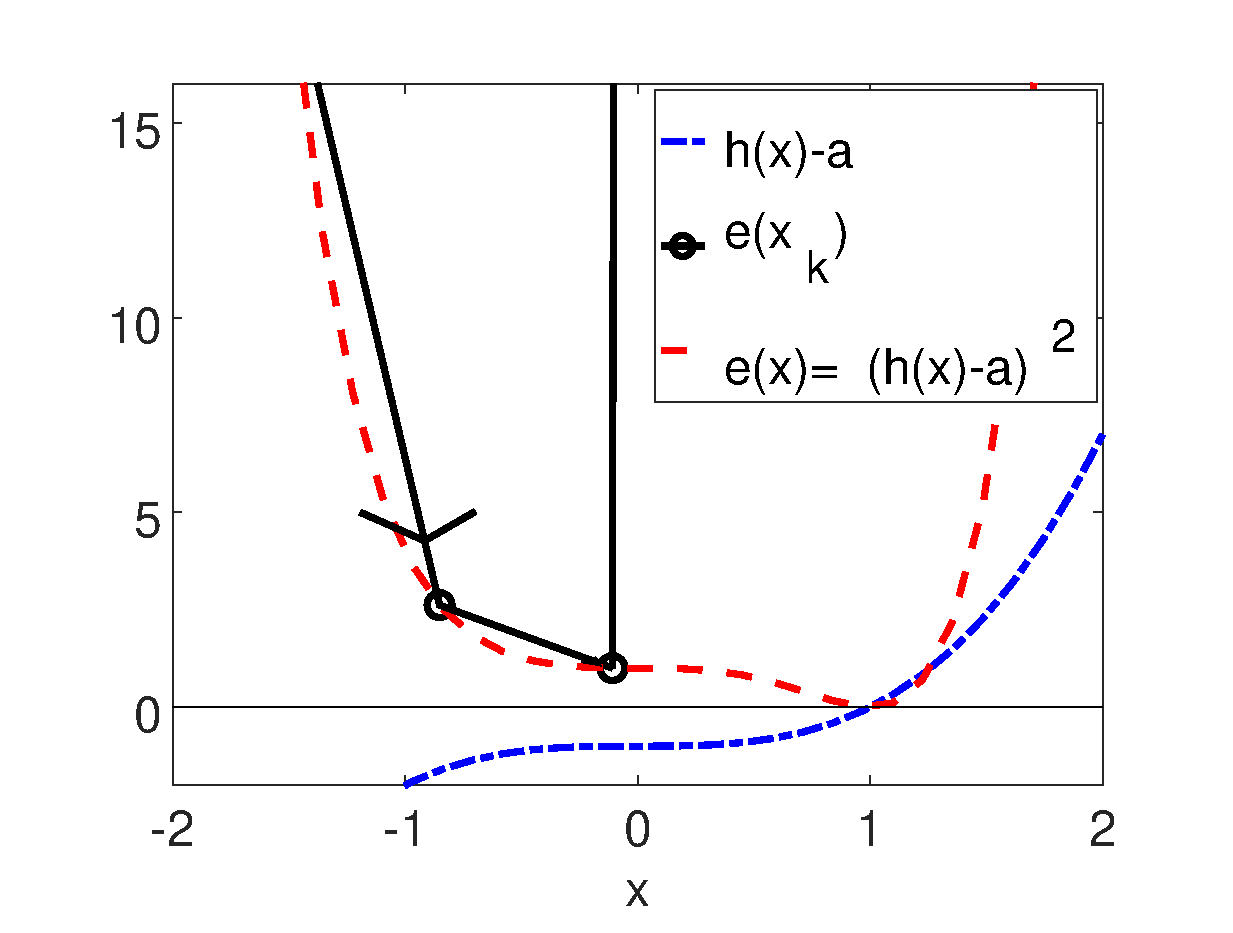
\includegraphics[width=\textwidth]{chapters/minimization-hx/mfiles/hx3_a/minimizando_hx_a_1.eps}
        \caption{Usando $h(x)=x^3$ e $a=1$, quando as iterações divergem}
        \label{fig:hxacases3a}
    \end{subfigure}
    ~ %add desired spacing between images, e. g. ~, \quad, \qquad, \hfill etc. 
      %(or a blank line to force the subfigure onto a new line)
    \begin{subfigure}[b]{0.49\textwidth}
        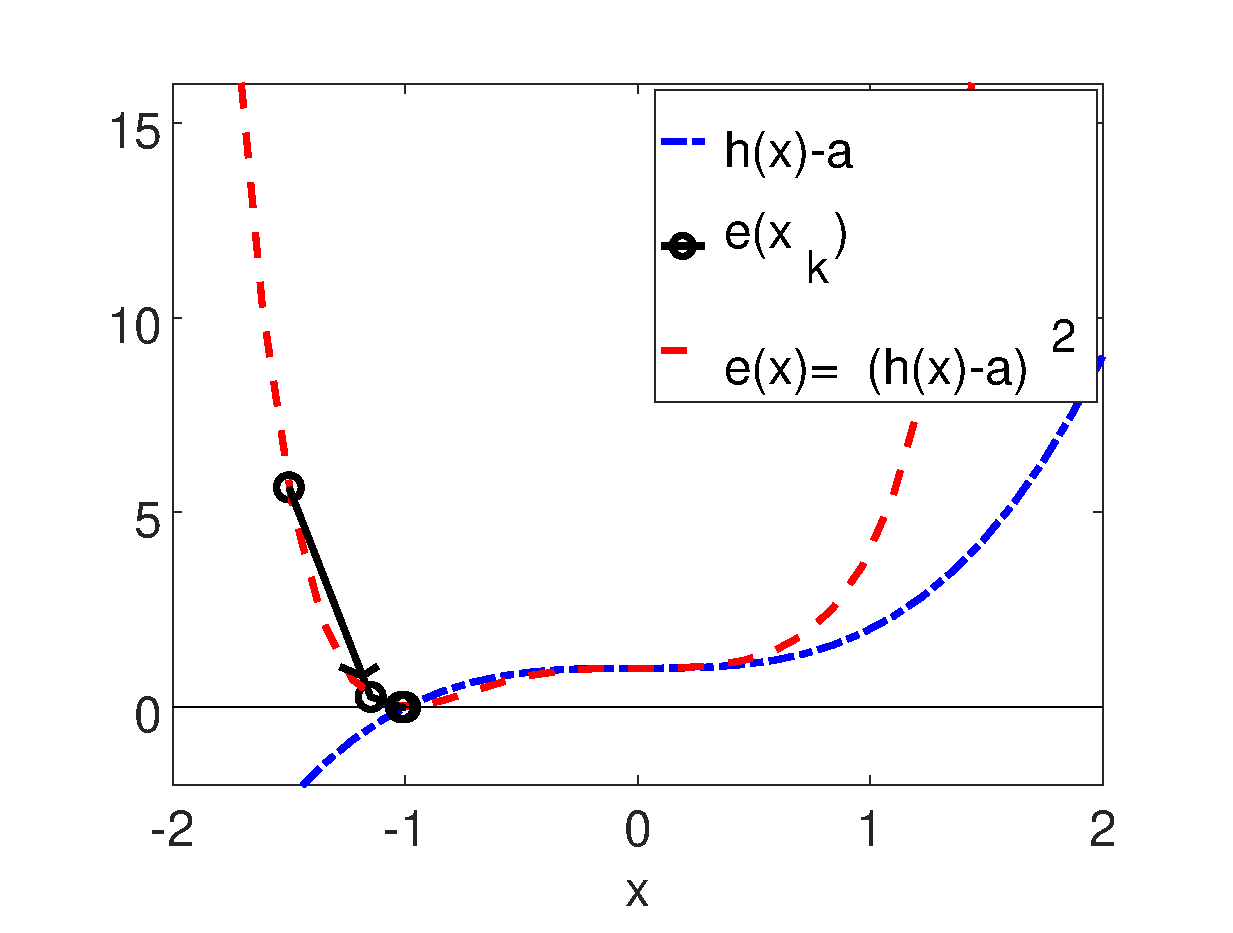
\includegraphics[width=\textwidth]{chapters/minimization-hx/mfiles/hx3_a/minimizando_hx_a_2.eps}
        \caption{Usando $h(x)=x^3$ e $a=-1$, quando as iterações convergem}
        \label{fig:hxacases3b}
    \end{subfigure}
    \caption{Comportamento para $h(x)=x^3$ da equação iterativa do Teorema \ref{theo:minhxhx}}
    \label{fig:hxacases3}
\end{figure}


\begin{table}[!h]
\centering
\begin{tabular}{|l|l|l|l|l|l|}
\hline
$k$      & 0 & 1 & 2 & 3 & 4 \\ \hline
$x_k$    & -1.50000 & -0.85185 & -0.10854 & 28.21988 & 18.81368 \\ \hline
$e(x_k)$ & 19.141 & 2.6184 & 1.0026 & 5.0500e+08 & 4.4331e+07 \\ \hline
\end{tabular}
\caption{Resposta iterativa do Exemplo \ref{ex:minhxhx3}.}
\label{tab:hxacases3}
\end{table}


\begin{example}\label{ex:minhxhx4}
Conhecida uma função $h(x)=x^3$ é valor $a=-1$ do contradomínio de $h(x)$,
achar o valor $\hat{x}$ que minimize $e(x)=(h(x)-a)^2$.
\end{example}
\begin{SolutionT}[Relativa ao Exemplo \ref{ex:minhxhx4}:]\label{sol:minhxhx4}
A Fig. \ref{fig:hxacases3b} nos mostra o processo de busca de um mínimo
 de $e(x)$, a busca inicia em $x_0=-1.5$,
 todos os valores de $x_{k}$ podem ser vistos na terceira coluna da
Tabela \ref{tab:hxacases4}. Neste caso a Eq. (\ref{eq:minhxhx2}) converge
em $\hat{x}\approx x_4 =-1$ com $e(\hat{x})\approx 0$, sendo este um mínimo global.
\end{SolutionT}

\begin{table}[!h]
\centering
\begin{tabular}{|l|l|l|l|l|l|}
\hline
$k$      & 0 & 1 & 2 & 3 & 4 \\ \hline
$x_k$    & -1.5000 & -1.1481 & -1.0183 & -1.0003 & -1.0000 \\ \hline
$e(x_k)$ & 5.6406e & 2.6372e-01 & 3.1238e-03 & 9.6110e-07 & 1.0241e-13 \\ \hline
\end{tabular}
\caption{Resposta iterativa do Exemplo \ref{ex:minhxhx4}.}
\label{tab:hxacases4}
\end{table}


\newpage

%%%%%%%%%%%%%%%%%%%%%%%%%%%%%%%%%%%%%%%%%%%%%%%%%%%%%%%%%%%%%%%%%%%%%%%%%%%%%%%%%%%%%%%
%%%%%%%%%%%%%%%%%%%%%%%%%%%%%%%%%%%%%%%%%%%%%%%%%%%%%%%%%%%%%%%%%%%%%%%%%%%%%%%%%%%%%%%
%%%%%%%%%%%%%%%%%%%%%%%%%%%%%%%%%%%%%%%%%%%%%%%%%%%%%%%%%%%%%%%%%%%%%%%%%%%%%%%%%%%%%%%
\section{Minimização de $||h(x)-a||^2+\alpha ||x-b||^2$}

\index{Problema inverso!Não linear}
\index{Minimização do erro quadrático!Não linear}

\begin{theorem}[Solução iterativa]\label{theo:minhxhxxbxb}
Dados,
um escalar $\alpha \in \mathbb{R} | \alpha > 0$, 
um escalar $x \in \mathbb{R}$, 
um escalar $a \in \mathbb{R}$,  
uma função $h:\mathbb{R} \rightarrow \mathbb{R}$, e 
definida a Eq. (\ref{eq:minhxhxxbxb1}),
\begin{equation}\label{eq:minhxhxxbxb1}
e(x)=||h(x)-a||^2+\alpha ||x-b||^2.
\end{equation}
Se desejamos ter o valor $\hat{x}$ que minimiza o escalar $e(\hat{x})$,
este valor pode ser achado\footnote{A 
demostração da Eq (\ref{eq:minhxhxxbxb2}) pode ser vista na Prova \ref{proof:theo:minhxhxxbxb}.} 
 usando iterativamente a Eq. (\ref{eq:minhxhxxbxb2}),
onde  $h'(x)\equiv \frac{d h(x)}{d x}$,
\begin{equation}\label{eq:minhxhxxbxb2}
x_{k} \leftarrow x_{k-1}-
\frac{ h'(x_{k-1}) \left[h(x_{k-1})-a\right]+\alpha\left[ x_{k-1}-b\right]}{\left[h'(x_{k-1})\right]^2+\alpha}.
\end{equation}
Assim, $\hat{x}$ pode ser achado iniciando a Eq. (\ref{eq:minhxhxxbxb2}) desde um 
$x_{0}$ qualquer, realizando cálculos $x_{k}$ iterativamente, 
ate que $x_{k}$ seja muito próximo a $x_{k-1}$ (convergência de $x_{k}$),
onde pode ser declarado que $\hat{x} \approx x_{k}$.

\textbf{Considerações:}
\begin{itemize}
\item É interessante verificar na Eq. (\ref{eq:minhxhxxbxb2}) 
se  $h'(x_{k-1}=b) = 0$,
pois indica que existe um ponto de inflexão 
(máximo, mínimo ou ponto de sela) em $e(x_{k-1}=b)$;
consequentemente poderiamos ter achado um mínimo\footnote{É 
interesante verificar o ponto $b$, uma vez só, 
antes de iniciar a busca iterativa.}.
\end{itemize}

\end{theorem}

\begin{tcbattention}
\begin{itemize}
\item O Teorema \ref{theo:minhxhxxbxb} pode ser usado para achar o ponto $x$
que minimize $e(x)=||h(x)-a||^2+\alpha||x-b||^2$,
quando sabemos que o vetor $x$ que minimiza $||h(x)-a||^2$ 
está perto do ponto $b$.
\item No Teorema \ref{theo:minhxhxxbxb} o ponto $x$ que minimiza $e(x)$, 
não necesariamente minimiza  $||h(x)-a||^2$.
\end{itemize}
\end{tcbattention}


%%%%%%%%%%%%%%%%%%%%%%%%%%%%%%%%%%%%%%%%%%%%%%%%%%%%%%%%%%%%%%%%%%%%%%%%%%%%%%%%
\subsection{Exemplos de minimização de $||h(x)-a||^2+\alpha ||x-b||^2$}


\begin{example}\label{ex:minhxhxxbxb1}
Conhecida uma função $h(x)=x^2(x^2-1)$, o valor $a=1$ do contradominio de $h(x)$,
o fator $\alpha=1.2$ e o ponto $b=0$,
achar o valor $\hat{x}$ que minimize $e(x)=||h(x)-a||^2+\alpha||x-b||^2$.
\end{example}
\begin{SolutionT}[Relativa ao Exemplo \ref{ex:minhxhxxbxb1}:]\label{sol:minhxhxxbxb1}


 A Fig. \ref{fig:hxbcasesa} nos mostra o processo de busca de um mínimo
 de $e(x)$. A busca inicia em $x_0=-1.4$,
 todos os valores $x_{k}$ podem ser vistos na Tabela \ref{tab:hxbcases1}. 
Neste caso a busca iterativa indicada pela Eq. (\ref{eq:minhxhxxbxb2}) converge sem problemas 
em $\hat{x}\approx x_7 =-1.21239$ com $e(x_7)=1.85954$; porem, 
 este valor de $x$ é um mínimo local e está longe do mínimo
 global de  $e(x)$ que está em $x=0$ com um $e(0)=1.0$.
\begin{comment}
 $x_7$ é um mínimo local de $e(x)$
 e está perto do mínimo global $x=\pm\sqrt{\frac{1+\sqrt{5}}{2}}\approx \pm1.2720$ 
de  $||h(x)-a||^2$; esta diferença é consequência do uso do fator 
 $\alpha>0$, pelo qual é de esperar que quanto maior seja o valor de $\alpha$
 maior será a diferencia da posição do mínimo global de $e(x)$ e de $||h(x)-a||^2$.
\end{comment}
\end{SolutionT}



\begin{table}[!h]
\centering
\begin{tabular}{|l|l|l|l|l|l|l|l|l|}
\hline
$k$      & 0 & 1 & 2 & 3 & 4 & 5 & 6 & 7 \\ \hline
$x_k$    & -1.4000 & -1.2694 & -1.2258 & -1.2153 & -1.2130 & -1.2125 & -1.2124 & -1.2124 \\ \hline
$e(x_k)$ & 3.1292 & 1.9338 & 1.8631 & 1.8597 & 1.8595 & 1.8595 & 1.8595 & 1.8595 \\ \hline
\end{tabular}
\caption{Resposta iterativa do Exemplo \ref{ex:minhxhxxbxb1}.}
\label{tab:hxbcases1}
\end{table}

\begin{figure}[!h]
    \centering
    \begin{subfigure}[b]{0.49\textwidth}
        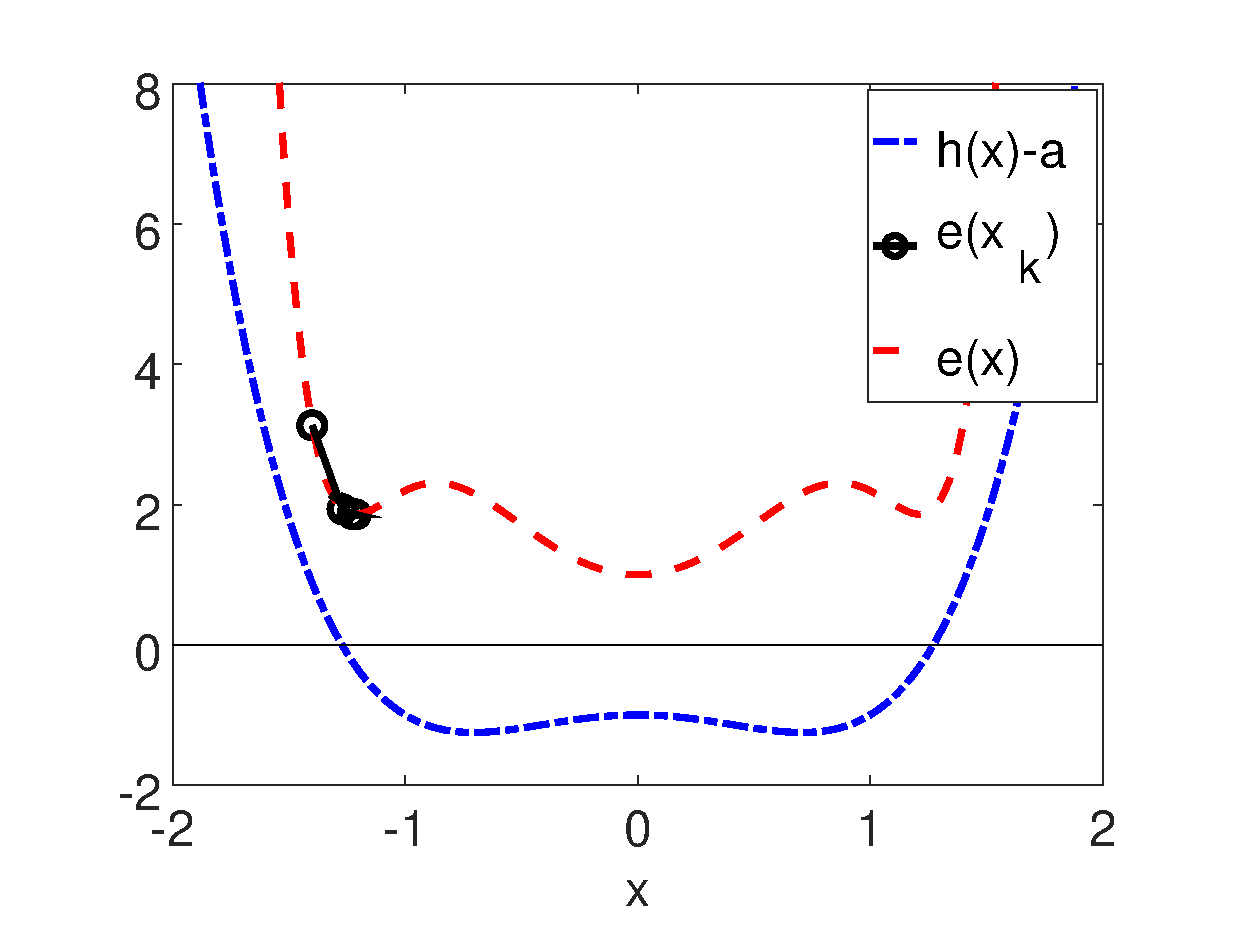
\includegraphics[width=\textwidth]{chapters/minimization-hx/mfiles/hx_a_alphax/minimizando_hx_a_alphax_1.eps}
        \caption{Usando $h(x)=x^2(x^2-1)$, $a=1$, $b=0$ e $\alpha=1.2$, quando as iterações convergem.}
        \label{fig:hxbcasesa}
    \end{subfigure}
    ~ %add desired spacing between images, e. g. ~, \quad, \qquad, \hfill etc. 
      %(or a blank line to force the subfigure onto a new line)
    \begin{subfigure}[b]{0.49\textwidth}
        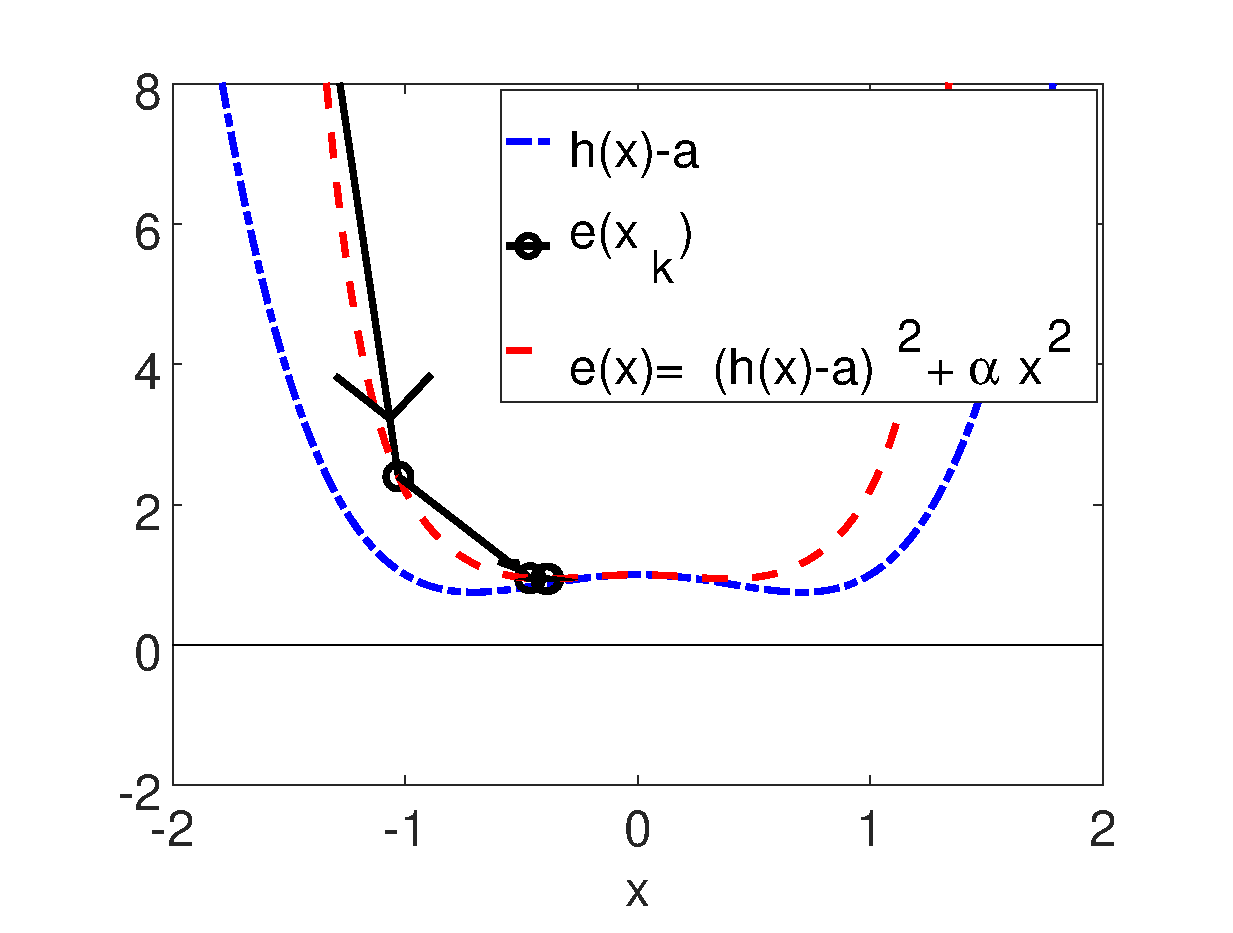
\includegraphics[width=\textwidth]{chapters/minimization-hx/mfiles/hx_a_alphax/minimizando_hx_a_alphax_2.eps}
        \caption{Usando $h(x)=x^2(x^2-1)$, $a=-1$, $b=0$ e $\alpha=1.2$, quando as iterações convergem.}
        \label{fig:hxbcasesb}
    \end{subfigure}
    \caption{Comportamento para $h(x)=x^2(x^2-1)$ da equação iterativa do Teorema \ref{theo:minhxhxxbxb}.}
    \label{fig:hxbcases}
\end{figure}


\begin{example}\label{ex:minhxhxxbxb2}
Conhecida uma função $h(x)=x^2(x^2-1)$, o valor $a=-1$ que não existe no contradominio de $h(x)$,
o fator $\alpha=1.2$ e o ponto $b=0$,
achar o valor $\hat{x}$ que minimize $e(x)=||h(x)-a||^2+\alpha||x-b||^2$.
\end{example}
\begin{SolutionT}[Relativa ao Exemplo \ref{ex:minhxhxxbxb2}:]\label{sol:minhxhxxbxb2}
 A Fig. \ref{fig:hxbcasesb} nos mostra o processo de busca de um mínimo
 de $e(x)$. A busca inicia em $x_0=-1.4$,
 todos os valores $x_{k}$ podem ser vistos na 
Tabela \ref{tab:hxbcases2}. Neste caso a busca iterativa indicada pela Eq. (\ref{eq:minhxhxxbxb2}) converge
em $\hat{x}\approx x_7=-0.39349$ com $e(\hat{x})=0.94120$ que é um mínimo global de $e(x)$.
\begin{comment}
; porem, este valor de $x_k$ está
um pouco distante do mínimo de $(h(x)-a)^2$, localizado em $x=\pm\frac{\sqrt{2}}{2}\approxeq \pm0.70711$.
Novamente, isto é consequência do uso do fator 
 $\alpha>0$, assim, quanto maior seja o valor de $\alpha$
 maior será a diferencia do mínimo global de $e(x)$ e de $(h(x)-a)^2$.
\end{comment}
\end{SolutionT}

\begin{table}[!h]
\centering
\begin{tabular}{|l|l|l|l|l|l|l|l|l|}
\hline
$k$      & 0 & 1 & 2 & 3 & 4 & 5 & 6 & 7 \\ \hline
$x_k$    & -1.4000 & -1.0290 & -0.4625 & -0.3849 & -0.3926 & -0.3934 & -0.3935 & -0.3935 \\ \hline
$e(x_k)$ & 10.65562 &  2.39969 &  0.94867 &  0.94130 &  0.94121 &  0.94120 &  0.94120 &  0.94120 \\ \hline
\end{tabular}
\caption{Resposta iterativa do Exemplo \ref{ex:minhxhxxbxb2}.}
\label{tab:hxbcases2}
\end{table}


\begin{example}\label{ex:minhx3hx3xbxb3}
Conhecida uma função $h(x)=(x+0.5)^3$, o valor $a=1$ no contradominio de $h(x)$,
o fator $\alpha=0.01$ e o ponto $b=0$,
achar o valor $\hat{x}$ que minimize $e(x)=||h(x)-a||^2+\alpha||x-b||^2$.
\end{example}
\begin{SolutionT}[Relativa ao Exemplo \ref{ex:minhx3hx3xbxb3}:]\label{sol:minhx3hx3xbxb3}
 A Fig. \ref{fig:hx3bcasesa} nos mostra o processo de busca de um mínimo
 de $e(x)$. 
 A busca inicia em $x_0=-1.4$,
 todos os valores $x_{k}$ podem ser vistos na Tabela \ref{tab:hx3bcases3}. 
Neste caso a busca iterativa indicada pela Eq. (\ref{eq:minhxhxxbxb2}) num principio diverge
em $x_2$, apos este evento as iterações continuam e estas convergem sem problemas 
em $\hat{x}\approx x_7=+0.53255$ com $e(\hat{x})\approx 0.013$.
\begin{comment}
; este valor de $x$ está perto do mínimo global de  $(h(x)-a)^2$, que está em  $x=+0.5$. 
Isto é consequência do uso do fator 
 $\alpha>0$ e pequeno, pelo qual é de esperar que quanto maior seja o valor de $\alpha$
 maior será a diferencia do mínimo global de $e(x)$ e de $(h(x)-a)^2$.
\end{comment}
\end{SolutionT}

\begin{table}[!h]
\centering
\begin{tabular}{|l|l|l|l|l|l|l|l|l|}
\hline
$k$      & 0 & 1 & 2 & 3 & 4 & 5 & 6 & 7 \\ \hline
$x_k$    & -1.400 & -0.68731 & 4.66500 & 2.95583 & 1.83178 & 1.11578 & 0.70475   & 0.53255 \\ \hline
$e(x_k)$ & 3.009 & 1.0179 & 1.8711e+4 & 1621.9 & 136.42 & 10.371 & 0.56538 & 0.013 \\ \hline
\end{tabular}
\caption{Resposta iterativa do Exemplo \ref{ex:minhx3hx3xbxb3}.}
\label{tab:hx3bcases3}
\end{table}

\begin{figure}[!h]
    \centering
    \begin{subfigure}[b]{0.49\textwidth}
        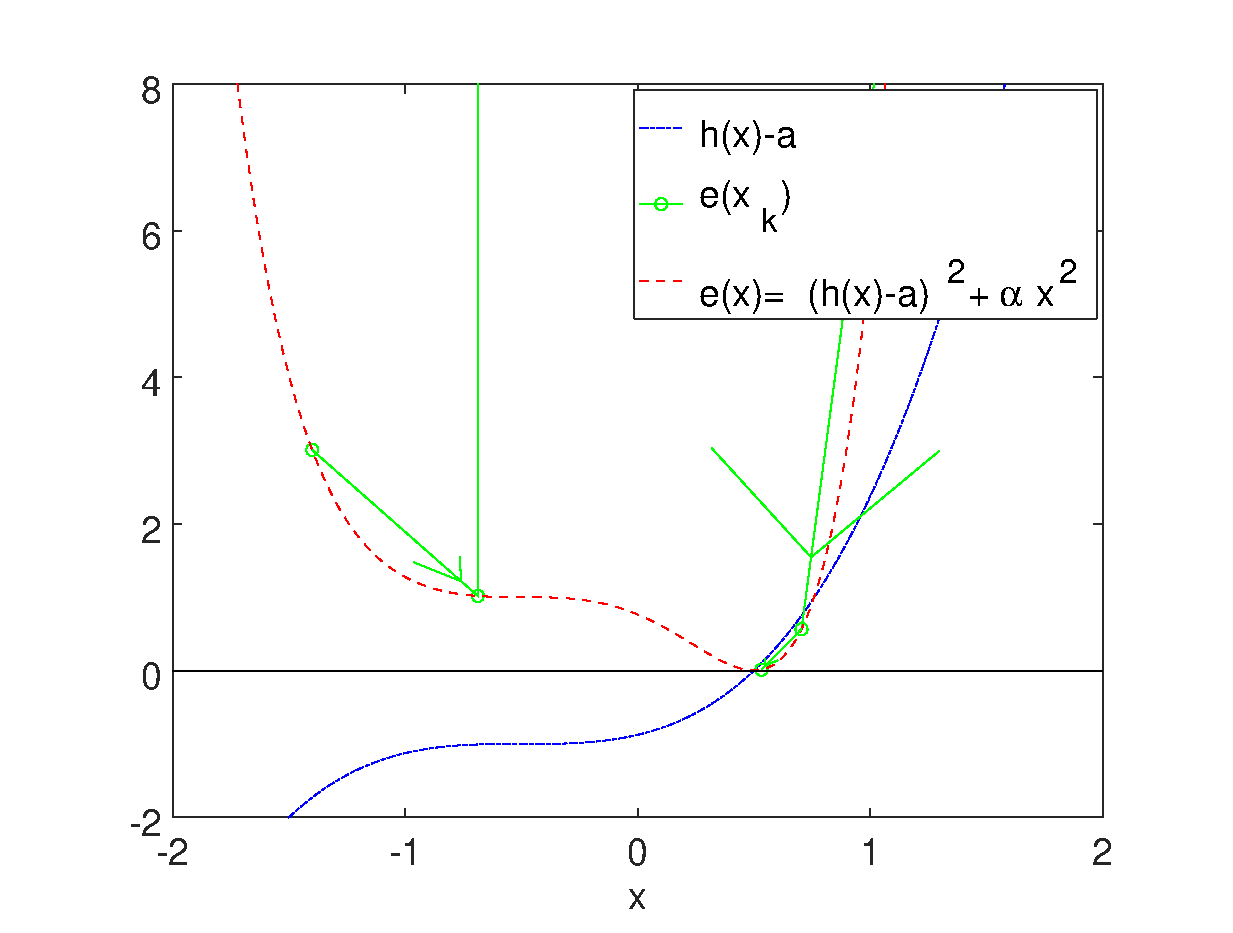
\includegraphics[width=\textwidth]{chapters/minimization-hx/mfiles/hx3_a_alphax/minimizando_hx_a_alphax_1.eps}
        \caption{Usando $h(x)=(x+0.5)^3$, $a=1$ e $\alpha=0.01$, quando as iterações divergem e logo convergem.}
        \label{fig:hx3bcasesa}
    \end{subfigure}
    ~ %add desired spacing between images, e. g. ~, \quad, \qquad, \hfill etc. 
      %(or a blank line to force the subfigure onto a new line)
    \begin{subfigure}[b]{0.49\textwidth}
        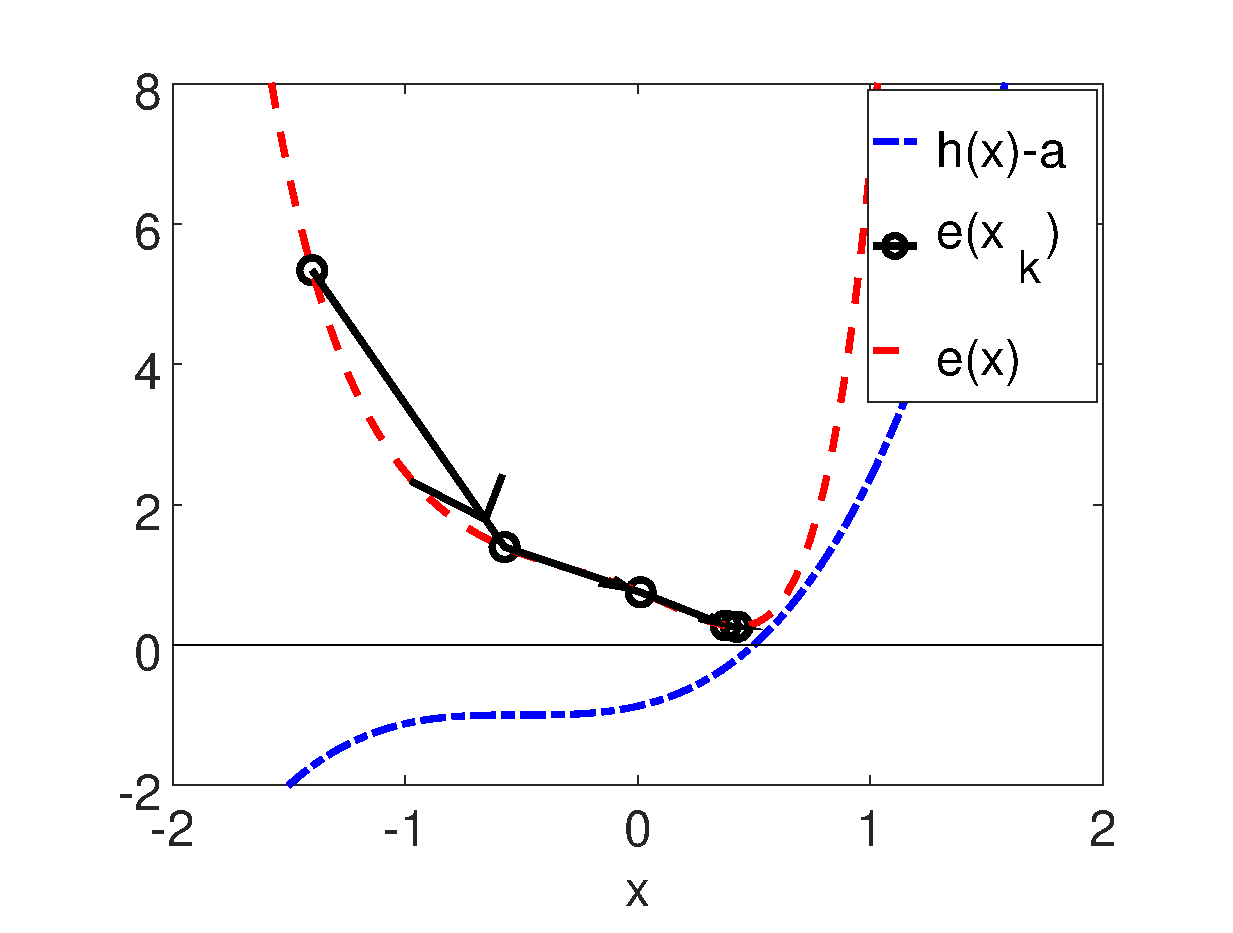
\includegraphics[width=\textwidth]{chapters/minimization-hx/mfiles/hx3_a_alphax/minimizando_hx_a_alphax_2.eps}
        \caption{Usando $h(x)=(x+0.5)^3$, $a=1$ e $\alpha=1.2$, quando as iterações convergem no mínimo global.}
        \label{fig:hx3bcasesb}
    \end{subfigure}
    \caption{Comportamento para $h(x)=(x+0.5)^3$ da equação iterativa do Teorema \ref{theo:minhxhxxbxb}.}
    \label{fig:hx3bcases}
\end{figure}

\begin{example}\label{ex:minhx3hx3xbxb4}
Conhecida uma função $h(x)=(x+0.5)^3$, o valor $a=1$ no contradominio de $h(x)$,
o fator $\alpha=1.2$ e o ponto $b=0$,
achar o valor $\hat{x}$ que minimize $e(x)=||h(x)-a||^2+\alpha||x-b||^2$.
\end{example}
\begin{SolutionT}[Relativa ao Exemplo \ref{ex:minhx3hx3xbxb4}:]\label{sol:minhx3hx3xbxb4}
 A Fig. \ref{fig:hx3bcasesb} nos mostra o processo de busca de um mínimo
 de $e(x)$. A busca inicia em $x_0=-1.4$,
 todos os valores $x_{k}$ podem ser vistos na Tabela \ref{tab:hx3bcases4}. 
Neste caso a busca iterativa indicada pela Eq. (\ref{eq:minhxhxxbxb2}) converge 
em $\hat{x}\approx x_7=+0.428757$ com $e(\hat{x})\approx 0.26$,
que é o mínimo global de $e(x)$.
\begin{comment}
; porem, este valor de $x_k$ está
um pouco distante do mínimo de $(h(x)-a)^2$, localizado em $x=+0.5$.
Novamente, isto é consequência do uso do fator 
 $\alpha>0$ e grande.
\end{comment}
\end{SolutionT}


\begin{table}[!h]
\centering
\begin{tabular}{|l|l|l|l|l|l|l|l|l|}
\hline
$k$      & 0 & 1 & 2 & 3 & 4 & 5 & 6 & 7 \\ \hline
$x_k$    & -1.40000 & -0.57219  & 0.01292  & 0.37895  & 0.42295  & 0.42797  & 0.42866  & 0.42876 \\ \hline
$e(x_k)$ &  5.34144 &  1.39364  & 0.74853  & 0.27534  & 0.26037  & 0.26015  & 0.26015  & 0.26015 \\ \hline
\end{tabular}
\caption{Resposta iterativa do Exemplo \ref{ex:minhx3hx3xbxb4}.}
\label{tab:hx3bcases4}
\end{table}



\newpage

%%%%%%%%%%%%%%%%%%%%%%%%%%%%%%%%%%%%%%%%%%%%%%%%%%%%%%%%%%%%%%%%%%%%%%%%%%%%%%%%%%%%%%%
%%%%%%%%%%%%%%%%%%%%%%%%%%%%%%%%%%%%%%%%%%%%%%%%%%%%%%%%%%%%%%%%%%%%%%%%%%%%%%%%%%%%%%%
%%%%%%%%%%%%%%%%%%%%%%%%%%%%%%%%%%%%%%%%%%%%%%%%%%%%%%%%%%%%%%%%%%%%%%%%%%%%%%%%%%%%%%%
\section{Minimização de $||h(x)-a||^2+\alpha ||x-x_{last}||^2$}

\index{Problema inverso!Não linear}
\index{Minimização do erro quadrático!Não linear}

\begin{theorem}[Solução iterativa]\label{theo:minhxhxxoxo}
Dados,
um escalar $\alpha \in \mathbb{R} | \alpha > 0$, 
um escalar $x \in \mathbb{R}$, 
um escalar $a \in \mathbb{R}$,  
uma função $h:\mathbb{R} \rightarrow \mathbb{R}$, e 
definida a Eq. (\ref{eq:minhxhxxoxo1}),
\begin{equation}\label{eq:minhxhxxoxo1}
e(x)=||h(x)-a||^2+\alpha ||x-x_{last}||^2,
\end{equation}
tendo em consideração que $x_{last}$ é uma constante equivalente a $x_{k-1}$
numa busca iterativa ou equivalente a $p$, 
se decidimos usar uma aproximação linear ao redor de $p$ em $h(x)$; 
é dizer, o segundo somando na Eq. (\ref{eq:minhxhxxoxo1}) 
procura minimizar $||x_{k}-x_{k-1}||^2$.

Se desejamos ter o valor $\hat{x}$ que minimiza o escalar $e(\hat{x})$,
este valor pode ser achado\footnote{A 
demostração da Eq (\ref{eq:minhxhxxoxo2}) pode ser vista na Prova \ref{proof:theo:minhxhxaxoxo}.} 
 usando iterativamente a Eq. (\ref{eq:minhxhxxoxo2}),
onde  $h'(x)\equiv \frac{d h(x)}{d x}$,
\begin{equation}\label{eq:minhxhxxoxo2}
x_{k+1} \leftarrow x_k+
\frac{ h'(x_k) \left[a-h(x_k)\right] }{\left[h'(x_k)\right]^2+\alpha},
\end{equation}
onde em cada iteração se tenta minimizar
\begin{equation}\label{eq:minhxhxxoxo2:ex}
e_{k-1}(x)  \equiv ||h(x)-a||^2 + \alpha||x-x_{k-1}||^2.
\end{equation}
Assim, $\hat{x}$ pode ser achado iniciando a Eq. (\ref{eq:minhxhxxoxo2}) desde um 
$x_{0}$ qualquer, realizando cálculos $x_{k}$ iterativamente, 
ate que $x_{k}$ seja muito próximo a $x_{k-1}$ (convergência de $x_{k}$),
onde pode ser declarado que $\hat{x} \approx x_{k}$.

\textbf{Considerações:}
\begin{itemize}
\item É interessante verificar sempre na Eq. (\ref{eq:minhxhxxoxo2}) 
se  $h'(x_{k-1}) = 0$,
pois indica que existe um ponto de inflexão 
(máximo, mínimo ou ponto de sela) em $e(x_{k-1})$;
consequentemente poderíamos ter achado um mínimo.
\end{itemize}

\end{theorem}

\begin{tcbattention}
\begin{itemize}
\item O Teorema \ref{theo:minhxhxxoxo} pode ser usado para achar o ponto $x$
que minimize $||h(x)-a||^2$, procurando 
em todo momento que na busca iterative se minimize $||x_{k}-x_{k-1}||^2$,
\end{itemize}
\end{tcbattention}
%%%%%%%%%%%%%%%%%%%%%%%%%%%%%%%%%%%%%%%%%%%%%%%%%%%%%%%%%%%%%%%%%%%%%%%%%%%%%%%%
\subsection{Exemplos de minimização de $||h(x)-a||^2+\alpha ||x-x_{last}||^2$}


\begin{example}\label{ex:minhxhxxoxo1}
Conhecida uma função $h(x)=x^2(x^2-1)$, o valor $a=1$ do contradominio de $h(x)$,
e o fator $\alpha=1.2$,
achar o valor $\hat{x}$ que minimize $e(x)=||h(x)-a||^2+\alpha||x-x_{last}||^2$.
\end{example}
\begin{SolutionT}[Relativa ao Exemplo \ref{ex:minhxhxxoxo1}:]\label{sol:minhxhxxoxo1}
 A Fig. \ref{fig:hxccasesa} nos mostra o processo de busca de um mínimo
 de $e(x)$. A busca inicia em $x_0=-1.4$,
 todos os valores $x_{k}$ podem ser vistos na Tabela \ref{tab:hxccases1}. 
Neste caso a busca iterativa indicada pela Eq. (\ref{eq:minhxhxxoxo2}) converge sem problemas 
em $\hat{x}\approx x_3 =-1.2721$ com $e(x_3)=8.7404e-08$.

É interesante lembrar que os valores $x_{min}=\pm \sqrt{\frac{1+\sqrt{5}}{2}}$ 
$\approx \pm 1.27202$ provocam $h(x_{min})=a$.
\end{SolutionT}

\begin{table}[!h]
\centering
\begin{tabular}{|l|l|l|l|l|}
\hline
$k$      & 0 & 1 & 2 & 3 \\ \hline
$x_k$    & -1.4000 & -1.2941 & -1.2734 & -1.2721 \\ \hline
$e_k(x_k)$ & 7.7722e-01 & 1.6835e-02 & 6.2390e-05 & 8.7404e-08 \\ \hline
\end{tabular}
\caption{Resposta iterativa do Exemplo \ref{ex:minhxhxxoxo1}.}
\label{tab:hxccases1}
\end{table}

\begin{figure}[!h]
    \centering
    \begin{subfigure}[b]{0.49\textwidth}
        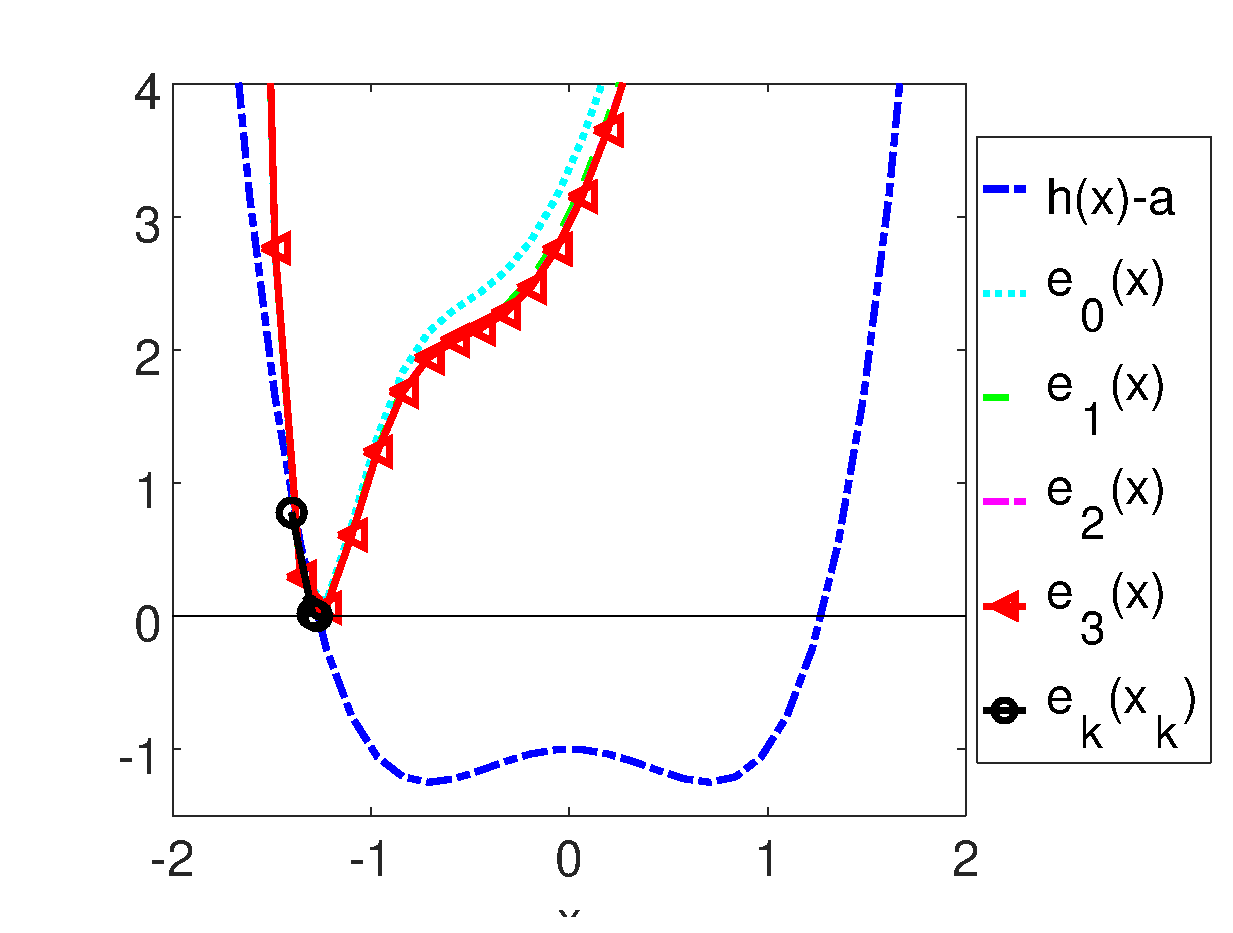
\includegraphics[width=\textwidth]{chapters/minimization-hx/mfiles/hx_a_alphax_last/minimizando_hx_a_alphax_1.eps}
        \caption{Usando $h(x)=x^2(x^2-1)$, $a=1$ e $\alpha=1.2$, quando as iterações convergem.}
        \label{fig:hxccasesa}
    \end{subfigure}
    ~ %add desired spacing between images, e. g. ~, \quad, \qquad, \hfill etc. 
      %(or a blank line to force the subfigure onto a new line)
    \begin{subfigure}[b]{0.49\textwidth}
        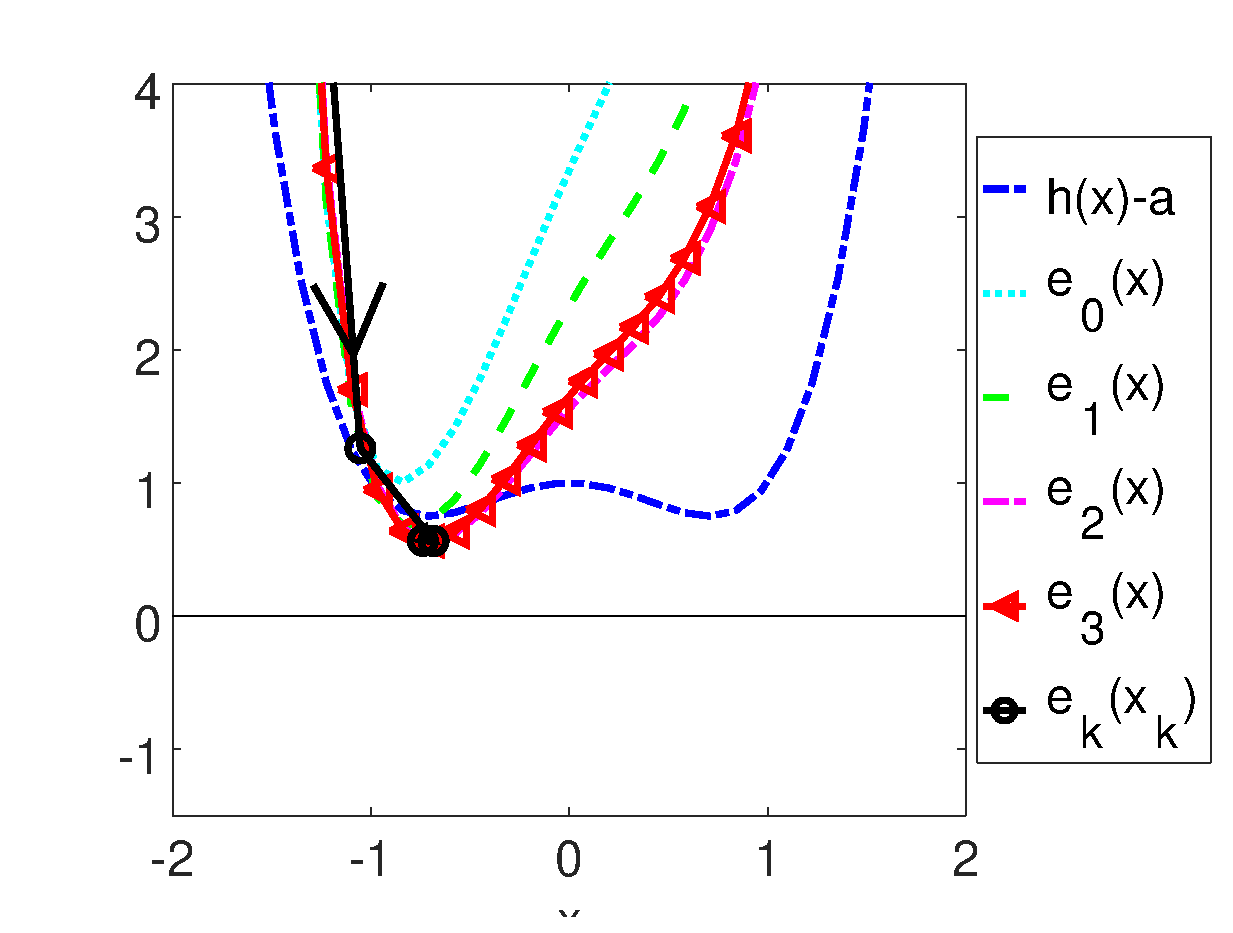
\includegraphics[width=\textwidth]{chapters/minimization-hx/mfiles/hx_a_alphax_last/minimizando_hx_a_alphax_2.eps}
        \caption{Usando $h(x)=x^2(x^2-1)$, $a=-1$ e $\alpha=1.2$, quando as iterações convergem.}
        \label{fig:hxccasesb}
    \end{subfigure}
    \caption{Comportamento para $h(x)=x^2(x^2-1)$ da equação iterativa do Teorema \ref{ex:minhxhxxoxo1}.}
    \label{fig:hxccases}
\end{figure}

\begin{example}\label{ex:minhxhxxoxo2}
Conhecida uma função $h(x)=x^2(x^2-1)$, o valor $a=-1$ que não existe no contradominio de $h(x)$,
e o fator $\alpha=1.2$,
achar o valor $\hat{x}$ que minimize $e(x)=||h(x)-a||^2+\alpha||x-x_{last}||^2$.
\end{example}
\begin{SolutionT}[Relativa ao Exemplo \ref{ex:minhxhxxoxo2}:]\label{sol:minhxhxxoxo2}
 A Fig. \ref{fig:hxccasesb} nos mostra o processo de busca de um mínimo
 de $e(x)$. A busca inicia em $x_0=-1.4$,
 todos os valores $x_{k}$ podem ser vistos na Tabela \ref{tab:hxccases2}. 
Neste caso a busca iterativa indicada pela Eq. (\ref{eq:minhxhxxoxo2}) converge sem problemas 
em $\hat{x}\approx x_3 =-0.73819$ com $e(x_3)=0.56553$.
\end{SolutionT}

\begin{table}[!h]
\centering
\begin{tabular}{|l|l|l|l|l|}
\hline
$k$      & 0 & 1 & 2 & 3 \\ \hline
$x_k$    & -1.40000 & -1.05377 & -0.68441 & -0.73819 \\ \hline
$e_k(x_k)$ & 8.30362 &  1.26028 &  0.56400 &  0.56553 \\ \hline
\end{tabular}
\caption{Resposta iterativa do Exemplo \ref{ex:minhxhxxoxo2}.}
\label{tab:hxccases2}
\end{table}


\newpage

\section{Provas dos teoremas}
 
%%%%%%%%%%%%%%%%%%%%%%%%%%%%%%%%%%%%%%%%%%%%%%%%%%%%%%%%%%%%%%%%%%%%%%%%%%%%%%%%%%%%%%%
%%%%%%%%%%%%%%%%%%%%%%%%%%%%%%%%%%%%%%%%%%%%%%%%%%%%%%%%%%%%%%%%%%%%%%%%%%%%%%%%%%%%%%%
\begin{myproofT}[Prova do Teorema \ref{theo:minhxhx}]\label{proof:theo:minhxhx}
Dados,
um escalar $x \in \mathbb{R}$, 
um escalar $a \in \mathbb{R}$,  
uma função $h:\mathbb{R} \rightarrow \mathbb{R}$, e 
definida a Eq. (\ref{eq:proof:minhxhx0}),
\begin{equation}\label{eq:proof:minhxhx0}
e(x)=||h(x)-a||^2.
\end{equation}
Para achar o valor  $\hat{x}$ que gere o menor valor de $e(x)$, é aplicado
o critério que um ponto de inflexão $x^+$ (máximo, mínimo ou ponto de sela) de $e(x)$ 
pode ser achado quando 
$\left. \frac{d e(x)}{d x }\right|_{x=x^+} \equiv e'(x^+) =0$.
Assim, 
usando o Teorema \ref{theo:derfxbCfxb0} podemos 
rescrever esta igualdade como a Eq. (\ref{eq:proof:minhxhxe}),
\begin{equation}\label{eq:proof:minhxhxe}
2  h'(x) \left[h(x) -a\right] = e'(x)=0,
\end{equation}
Da Eq. (\ref{eq:proof:minhxhxe}), observamos 
que existem duas formas de achar um ponto de inflexão $x^+$,
\begin{itemize}
 \item a primeira forma a achamos se temos um valor $x^+$ tal que $h'(x^+)=0$, 
que representa um ponto de inflexão simultâneo em $e(x)$ e $h(x)$, e
 \item a segunda forma é achando um valor $x^+$ tal que $h(x^+)=a$;
que representa um ponto de inflexão de $e(x)$, mas não
necessariamente de $h(x)$; 
sendo este ponto $x^+=\hat{x}$ também um mínimo absoluto, pois provocam $e(\hat{x})=0$.
\end{itemize}




Por outro lado, podemos realizar uma aproximação linear de $h(x)$ em $e(x)$
ao redor do ponto $p$, usando a \hyperref[def:taylor]{\textbf{serie de Taylor}},
de modo que a Eq. (\ref{eq:proof:minhxhx0}) pode ficar expressada como
\begin{equation}\label{eq:proof:minhxhxe:approx0}
e(x) \approx  e_p(x) = ||h'(p)\{x-p\}-\{a-h(p)\}||^2.
\end{equation}
Assim, da Eq. (\ref{eq:proof:minhxhxe:approx0})
podemos concluir que um ponto $x^*$ que é 
um mínimo da aproximação linear $e_p(x)$ feita em $e(x)$ ao redor do ponto $p$,
pode ser achado como
\begin{equation}\label{eq:proof:minhxhx2}
 h'(p)\{x^*-p\} = \{a-h(p)\} \qquad \leftrightarrow \qquad x^* = p - \frac{h(p)-a}{ h'(p)}.
\end{equation} 

Desta equação podemos tirar a seguintes conclusões:
\begin{itemize}

\item Observamos que a posição $p$ é corregida para ficar próximo à posição $x^*$, 
que é um mínimo absoluto de $e_p(x)$ na direção de um mínimo (qualquer) de $e(x)$;
pelo que se deduz que a Eq. (\ref{eq:proof:minhxhx2})
pode ser usada para procurar aproximações $x^*$ de pontos mínimos $\hat{x}$ em $e(x)$ desde a posição $p$;
ou pelo menos aproximações de novas posições em caminhos numa direção descendente de $e(x)$.

\item A Eq. (\ref{eq:proof:minhxhx2}) é satisfeita 
com $x^* \approx p$ se acharmos um  
ponto $p$ onde  $a \approx h(p)$; 
é dizer um mínimo global de $e(x)$ em $p$.%, como pode ser visto na Figura \ref{fig:ex0a}. 

\item Dado que a Eq. (\ref{eq:proof:minhxhx2}) tem um termo $h'(p)$ no denominador,
valores $p$ que cumpram $h'(p)\approx 0$ provocam uma correção distante (divergência) da posição $p$,
nos casos onde $p$ se aproxime a máximos e pontos de sela,
ou mínimos locais. 
Mas sim se trata de um mínimo global com $h(p)\approx a$, 
o comportamento será inesperado e dependerá se é finito ou não, o
\begin{equation}
lim_{x\rightarrow p } \frac{h(p)-a}{h'(p)}.
\end{equation}

\item Se modificamos a Eq. (\ref{eq:proof:minhxhx2}), e escolhemos um ponto  
$p_0$ que consideremos próximo ao ponto $\hat{x}$ que minimiza $e(\hat{x})$,
podemos achar iterativamente aproximações lineares $x^*$ cada vez mais próximos a  $\hat{x}$,
se usamos a seguinte equação iterativa,
\begin{equation}\label{eq:proof:minhxhx3}
p_{k} \leftarrow p_{k-1} - \frac{ h(p_{k-1})-a}{h'(p_{k-1})},
\end{equation}
iniciando desde um $p_{0}$ 
ate que exista uma tendencia prolongada onde se observe que $p_{k}$ é muito próximo a $p_{k-1}$,
momento no qual declaramos que $\hat{x} \approx p_{k}$.
\item Pode existir um mínimo global $\hat{x}$ de $e(\hat{x})>0$.
Isto nos restringe a que no uso da Eq. (\ref{eq:proof:minhxhx3}),
nosso critério principal para estabelecer o final do cáculo iterativo,
deve ser a tendencia na  proximidade entre $p_{k}$ e $p_{k-1}$ 
e não o valor de $e(x_k)$.
\end{itemize}

Um diagrama completo resumindo todas estas conclusões pode ser visto na Figura \ref{fig:fluxohx1}.
\end{myproofT}



\begin{figure}[!h]
     \centering
         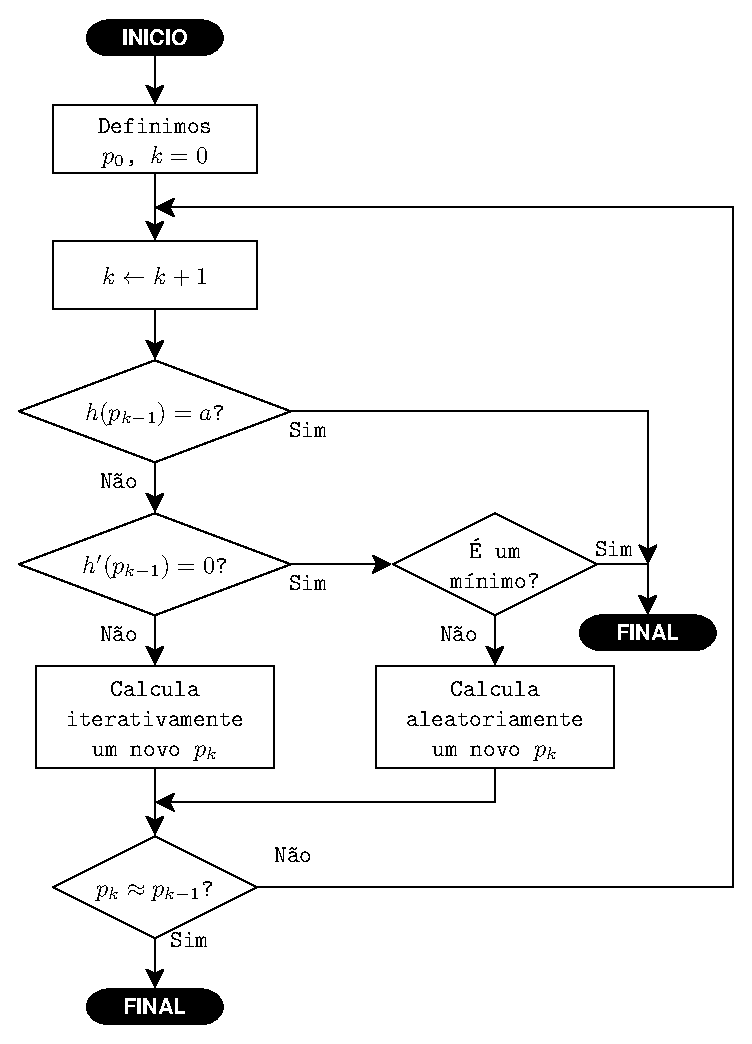
\includegraphics[width=0.75\textwidth]{chapters/minimization-hx/fluxo1.eps}
        \caption{Diagrama de fluxo da solução iterativa para achar um mínimo, seguindo a Prova \ref{proof:theo:minhxhx}.}
        \label{fig:fluxohx1}
\end{figure}


%%%%%%%%%%%%%%%%%%%%%%%%%%%%%%%%%%%%%%%%%%%%%%%%%%%%%%%%%%%%%%%%%%%%%%%%%%%%%%%%%%%%%%%
%%%%%%%%%%%%%%%%%%%%%%%%%%%%%%%%%%%%%%%%%%%%%%%%%%%%%%%%%%%%%%%%%%%%%%%%%%%%%%%%%%%%%%%
\begin{myproofT}[Prova do Teorema \ref{theo:minhxhxxbxb}]\label{proof:theo:minhxhxxbxb}

Dados,
um escalar $x \in \mathbb{R}$, 
um escalar $a \in \mathbb{R}$,
um escalar $\alpha \in \mathbb{R}^{+}$,
um escalar $b \in \mathbb{R}$,
uma função $h:\mathbb{R} \rightarrow \mathbb{R}$, e 
definida a Eq. (\ref{eq:proof:minhxhxxbxb0}),
\begin{equation}\label{eq:proof:minhxhxxbxb0}
e(x)=||h(x)-a||^2+\alpha ||x-b||^2.
\end{equation}

Para achar o valor  $\hat{x}$ que gere o menor valor de $e(x)$, é aplicado
o critério que um ponto de inflexão $x^+$ (máximo, mínimo ou ponto de sela) de $e(x)$ 
pode ser achado quando 
$\left. \frac{d e(x)}{d x }\right|_{x=x^+} \equiv e'(x^+) =0$.
Assim, 
usando o Teorema \ref{theo:derfxbCfxb0} e \ref{theo:derAxbAxb}  podemos 
rescrever esta igualdade como a Eq. (\ref{eq:proof:minhxhxxbxbe}),
\begin{equation}\label{eq:proof:minhxhxxbxbe}
2  h'(x) \left[h(x) -a\right]+2\alpha (x-b)= e'(x)=0,
\end{equation}
Da Eq. (\ref{eq:proof:minhxhxxbxbe}), observamos 
que existem duas formas de achar um ponto de inflexão $x^+$,
\begin{itemize}
 \item a primeira forma a achamos se temos um valor $x^+=b$ tal que $h'(b)=0$, 
que representa um ponto de inflexão simultâneo em $e(x)$ e $h(x)$, e
 \item a segunda forma é achando um valor $x^+=b$ tal que $h(b)=a$;
que representa um ponto de inflexão de $e(x)$, mas não
necessariamente de $h(x)$; 
sendo este ponto $x^+=\hat{x}=b$ também um mínimo absoluto, pois provocam $e(\hat{x})=0$.
\end{itemize}

Por outro lado, podemos realizar uma aproximação linear de $h(x)$ em $e(x)$
ao redor do ponto $p$, usando a \hyperref[def:taylor]{\textbf{serie de Taylor}},
de modo que a Eq. (\ref{eq:proof:minhxhxxbxb0}) pode ficar expressada como
\begin{equation}\label{eq:proof:minhxhxxbxbe:approx0}
e(x) \approx  e_p(x) = ||h'(p)\{x-p\}-\{a-h(p)\}||^2+\alpha ||x-b||^2.
\end{equation}
Assim, da Eq. (\ref{eq:proof:minhxhxxbxbe:approx0})
podemos concluir que um ponto $x^*$ que é 
o mínimo da aproximação linear $e_p(x)$ feita em $e(x)$ ao redor do ponto $p$,
pode ser achado aplicando $\left. \frac{d e_p(x)}{d x }\right|_{x=x^*} \equiv e_{p}'(x^*) =0$,
de modo que obtemos
\begin{equation}\label{eq:proof:minhxhxaxb2a}
 2 h'(p)[h'(p)\{x^*-p\} -\{a-h(p)\}] + \alpha [x^*-b] = 0,
\end{equation} 
\begin{equation}\label{eq:proof:minhxhxaxb2}
x^* = p - \frac{h'(p)\{h(p)-a\}+\alpha\{p-b\}}{ h'(p)^2+\alpha}.
\end{equation} 

Desta equação podemos tirar a seguintes conclusões:


\begin{itemize}

\item Observamos que a posição $p$ é corregida para ficar próximo à posição $x^*$, 
que é um mínimo absoluto de $e_p(x)$ na direção de um mínimo (qualquer) de $e(x)$;
pelo que se deduz que a Eq. (\ref{eq:proof:minhxhxaxb2})
pode ser usada para procurar aproximações $x^*$ de pontos mínimos $\hat{x}$ em $e(x)$ desde a posição $p$;
ou pelo menos aproximações de novas posições em caminhos numa direção descendente de $e(x)$.

\begin{comment}
\item A Eq. (\ref{eq:proof:minhxhxaxb2}) é satisfeita 
com $x^* \approx p$ se acharmos um  
ponto $p=b$ onde  $a \approx h(b)$; 
é dizer um mínimo global de $e(x)$ em $b$.%, como pode ser visto na Figura \ref{fig:ex0a}. 
\item A Eq. (\ref{eq:proof:minhxhxaxb2}) é satisfeita 
com $x^* \approx p$ se acharmos um  
ponto $p=b$ onde  $0 \approx h'(b)$; 
é dizer um ponto de inflexão de $e(x)$ em $b$.
\end{comment}

\item Se reescrevemos a Eq. (\ref{eq:proof:minhxhxaxb2}) usando o Teorema \ref{theo:derfxbCfxb0}
e o Corolário \ref{coro:derAxbAxb2},
obtemos
\begin{equation}\label{eq:proof:minhxhxaxbea1}
x^* \approx p -
\frac{ e'(p)}{2 \{h'(p)^2+\alpha\} },
\end{equation}
onde a Eq. (\ref{eq:proof:minhxhxaxbea1}) é satisfeita 
com $x^* \approx p$
se acharmos um  ponto $p$ onde  
$e'(p)\approx 0$; 
é dizer $p$ é um ponto de inflexão de $e(x)$, como já foi analisado na Eq. (\ref{eq:proof:minhxhxxbxbe}).
%como pode ser visto na Figura \ref{fig:ex0b}.
Porem, dado que a Eq. (\ref{eq:proof:minhxhxaxbea1}) avança desde $p$ na direção de um mínimo $x^*$, 
mesmo que nos pontos de inflexão correspondentes a máximos ou pontos de sela,
encontremos valores de $p$ próximos a $x^*$,
 estes casos serão pouco estáveis pois
a correção da posição $p$ será na direção de um mínimo e não do máximo.

\item Se modificamos a Eq. (\ref{eq:proof:minhxhxaxb2}), e escolhemos um ponto  
$p_0$ que consideremos próximo ao ponto $\hat{x}$ que minimiza $e(\hat{x})$,
podemos achar iterativamente aproximações lineares $x^*$ cada vez mais próximos a  $\hat{x}$,
se usamos a seguinte equação iterativa,
\begin{equation}\label{eq:proof:minhxhxaxb3}
p_{k} \leftarrow p_{k-1} - \frac{ h'(p_{k-1})\{h(p_{k-1})-a\}+\alpha\{p-b\}}{h'(p_{k-1})^2+\alpha},
\end{equation}
iniciando desde um $p_{0}$ 
ate que exista uma tendencia prolongada onde se observe que $p_{k}$ é muito próximo a $p_{k-1}$,
momento no qual declaramos que $\hat{x} \approx p_{k}$.
\item Pode existir um mínimo global $\hat{x}$ de $e(\hat{x})>0$.
Isto nos restringe a que no uso da Eq. (\ref{eq:proof:minhxhxaxb3}),
nosso critério principal para estabelecer o final do cáculo iterativo,
deve ser a tendencia na  proximidade entre $p_{k}$ e $p_{k-1}$ 
e não o valor de $e(x_k)$.
\end{itemize}

Um diagrama completo resumindo todas estas conclusões pode ser visto na Figura \ref{fig:fluxohx2}.
\end{myproofT}



\begin{figure}[!h]
     \centering
         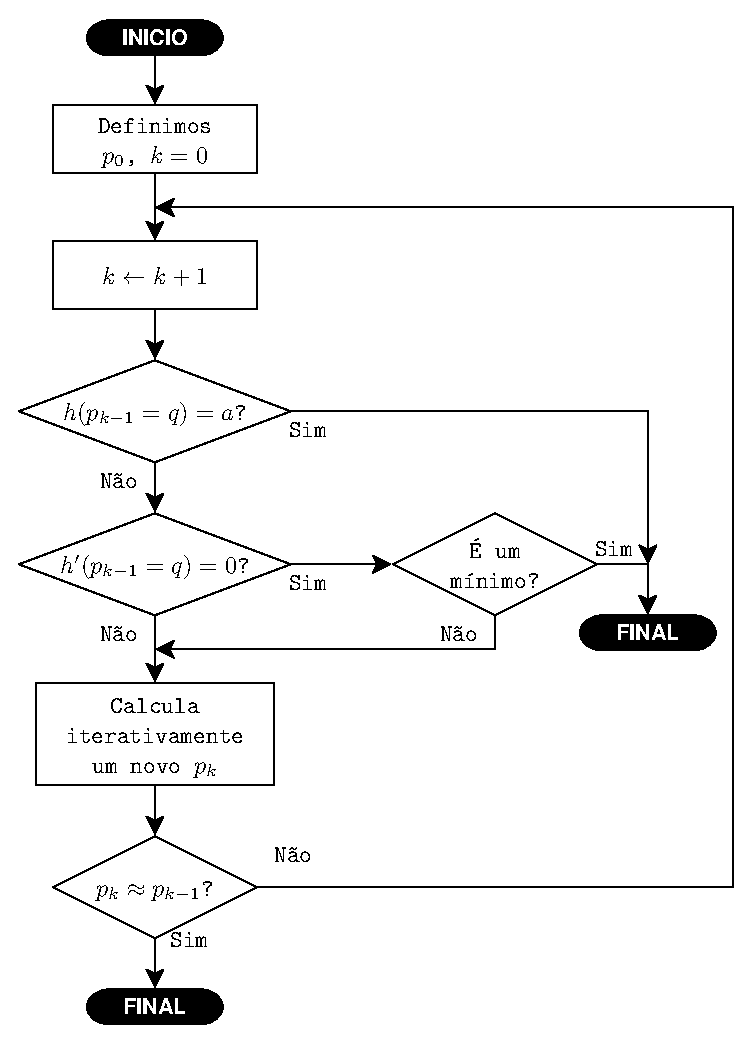
\includegraphics[width=0.75\textwidth]{chapters/minimization-hx/fluxo2.eps}
        \caption{Diagrama de fluxo da solução iterativa para achar um mínimo, seguindo a Prova \ref{proof:theo:minhxhxxbxb}.}
        \label{fig:fluxohx2}
\end{figure}


%%%%%%%%%%%%%%%%%%%%%%%%%%%%%%%%%%%%%%%%%%%%%%%%%%%%%%%%%%%%%%%%%%%%%%%%%%%%%%%%%%%%%%%
%%%%%%%%%%%%%%%%%%%%%%%%%%%%%%%%%%%%%%%%%%%%%%%%%%%%%%%%%%%%%%%%%%%%%%%%%%%%%%%%%%%%%%%
\begin{myproofT}[Prova do Teorema \ref{theo:minhxhxxoxo}]\label{proof:theo:minhxhxaxoxo}

Dados,
um escalar $x \in \mathbb{R}$, 
um escalar $a \in \mathbb{R}$,
um escalar $\alpha \in \mathbb{R}^{+}$,
um escalar $x_{last} \in \mathbb{R}$,
uma função $h:\mathbb{R} \rightarrow \mathbb{R}$, e 
definida a Eq. (\ref{eq:proof:minhxhxxoxo0}),
\begin{equation}\label{eq:proof:minhxhxxoxo0}
e(x)=||h(x)-a||^2+\alpha ||x-x_{last}||^2.
\end{equation}
tendo em consideração que $x_{last}$ é uma constante equivalente a $x_{k-1}$
numa busca iterativa ou equivalente a $p$, 
se decidimos usar uma aproximação linear ao redor de $p$ em $h(x)$; 
é dizer, o segundo somando na Eq. (\ref{eq:proof:minhxhxxoxo0}) 
procura minimizar $||x_{k}-x_{k-1}||^2$.


Para achar o valor  $\hat{x}$ que gere o menor valor de $e(x)$, é aplicado
o critério que um ponto de inflexão $x^+$ (máximo, mínimo ou ponto de sela) de $e(x)$ 
pode ser achado quando 
$\left. \frac{d e(x)}{d x }\right|_{x=x^+} \equiv e'(x^+) =0$.
Assim, 
usando o Teorema \ref{theo:derfxbCfxb0} e \ref{theo:derAxbAxb}  podemos 
rescrever esta igualdade como a Eq. (\ref{eq:proof:minhxhxxoxoe}),
\begin{equation}\label{eq:proof:minhxhxxoxoe}
2  h'(x) \left[h(x) -a\right]+2\alpha (x-x_{last})= e'(x)=0,
\end{equation}
Da Eq. (\ref{eq:proof:minhxhxxoxoe}), observamos 
que existem duas formas de achar um ponto de inflexão $x^+$,
\begin{itemize}
 \item a primeira forma a achamos se temos um valor $x^+=x_{last}$ tal que $h'(x_{last})=0$, 
que representa um ponto de inflexão simultâneo em $e(x)$ e $h(x)$, e
 \item a segunda forma é achando um valor $x^+=x_{last}$ tal que $h(x_{last})=a$;
que representa um ponto de inflexão de $e(x)$, mas não
necessariamente de $h(x)$; 
sendo este ponto $x^+=\hat{x}=x_{last}$ também um mínimo absoluto, pois provocam $e(\hat{x})=0$.
\end{itemize}

Por outro lado, procurando outros critérios para achar os pontos de inflexão,
podemos igualar $x_{last}\equiv p$ e 
realizar uma aproximação linear de $h(x)$ em $e(x)$
ao redor do ponto $p$ usando a \hyperref[def:taylor]{\textbf{serie de Taylor}},
de modo que a Eq. (\ref{eq:proof:minhxhxxoxo0}) pode ficar expressada como
\begin{equation}\label{eq:proof:minhxhxxoxo0approx}
e(x) \approx e_{p}(x)  \equiv ||h'(p)[x-p]-[a-h(p)]||^2+\alpha||x-p||^2,
\end{equation}


%%%%%%%
Assim, usando o resultado da Prova \ref{proof:theo:minAxbCAxbalphaxqD} na Eq. (\ref{eq:proof:minhxhxxoxo0approx}), 
podemos concluir que um ponto $x^*$ que é 
o mínimo da aproximação linear $e_p(x)$ feita em $e(x)$ ao redor do ponto $p$,
pode ser achado aplicando $\left. \frac{d e_p(x)}{d x }\right|_{x=x^*} \equiv e_{p}'(x^*) =0$,
de modo que obtemos
\begin{equation}\label{eq:proof:minhxhxaxo2a}
 2 h'(p)[h'(p)\{x^*-p\} -\{a-h(p)\}] + \alpha [x^*-p] = 0,
\end{equation} 
\begin{equation}\label{eq:proof:minhxhxaxo2}
x^* = p - \frac{h'(p)\{h(p)-a\}}{ h'(p)^2+\alpha}.
\end{equation} 








Desta equação podemos tirar a seguintes conclusões:
\begin{itemize}

\item Observamos que a posição $p$ é corregida para ficar próximo à posição $x^*$, 
que é o valor mínimo na aproximação linear ao redor de $p$;
pelo que se deduz que a Eq. (\ref{eq:proof:minhxhxaxo2})
pode ser usada para procurar aproximações de pontos mínimos $\hat{x}$ em $e(x)$ desde a posição $p$,
ou pelo menos aproximações de novas posições em caminhos numa direção descendente de $e(x)$.

\begin{comment}
\item A Eq. (\ref{eq:proof:minhxhxaxo2}) é satisfeita 
com $x^* \approx p$ se acharmos um  
ponto $p$ onde  $a \approx h(p\approx x_{last})$; 
é dizer um mínimo global de $e(x)$ em $p$. 
\end{comment}

\item Se reescrevemos a Eq. (\ref{eq:proof:minhxhxaxo2}) usando o Teorema \ref{theo:derfxbCfxb0}
e o Corolário \ref{coro:derAxbAxb2},
obtemos
\begin{equation}\label{eq:proof:minhxhxaxoxo2ea1}
x^* \approx p - \frac{ e'(p)}{2(h'(p)^2+\alpha)},
\end{equation}
onde a Eq. (\ref{eq:proof:minhxhxaxoxo2ea1}) é satisfeita 
com $x^* \approx p$
se acharmos um  ponto $p$ onde  
$e'(p)\approx 0$; 
é dizer $p$ é um ponto de inflexão de $e(x)$, como pode ser visto na Eq. (\ref{eq:proof:minhxhxxoxoe}).
Porem, dado que a Eq. (\ref{eq:proof:minhxhxaxoxo2ea1}) avança desde $p$ na direção de um mínimo $x^*$, 
mesmo que nos pontos de inflexão correspondentes a máximos ou pontos de sela,
encontremos valores de $p$ próximos a $x^*$,
 estes casos serão pouco estáveis pois
a correção da posição $p$ será na direção de um mínimo e não do máximo.

\item Se modificamos a Eq. (\ref{eq:proof:minhxhxaxo2}), e escolhemos um ponto  
$p_0$ que consideremos próximo ao ponto $\hat{x}$ que minimiza $e(\hat{x})$,
podemos achar iterativamente aproximações lineares $x^*$ cada vez mais próximos a  $\hat{x}$,
se usamos a seguinte equação iterativa,
\begin{equation}\label{eq:proof:minhxhxaxoxo3b}
p_{k} \leftarrow p_{k-1} - \frac{h'(p_{k-1})\{h(p_{k-1})-a\}}{h'(p_{k-1})^2 +\alpha},
\end{equation}
onde se inicia desde um $p_{0}$ 
ate que exista uma tendencia prolongada onde se observe que $p_{k}$ é muito próximo a $p_{k-1}$,
momento no qual declaramos que $\hat{x} \approx p_{k}$.
Disto também se deduz que o erro a minimizar em cada iteração será diferente e influenciado pelo valor do ponto $p_{k-1}$,
\begin{equation}
e_{k-1}(x)  \equiv ||h(x)-a||^2+\alpha||x-p_{k-1}||^2
\end{equation}
\item Pode existir um mínimo global $\hat{x}$ de $e(\hat{x}) > 0$.
Isto nos restringe a que no uso da Eq. (\ref{eq:proof:minhxhxaxoxo3b}),
nosso critério principal para estabelecer o final do cáculo iterativo,
deve ser a tendencia na  proximidade entre $p_{k}$ e $p_{k-1}$ 
e não o valor de $e(x_k)$.
\end{itemize}~

Um diagrama completo resumindo todas estas conclusões pode ser visto na Figura \ref{fig:fluxohx3}.
\end{myproofT}
\begin{figure}[!h]
     \centering
         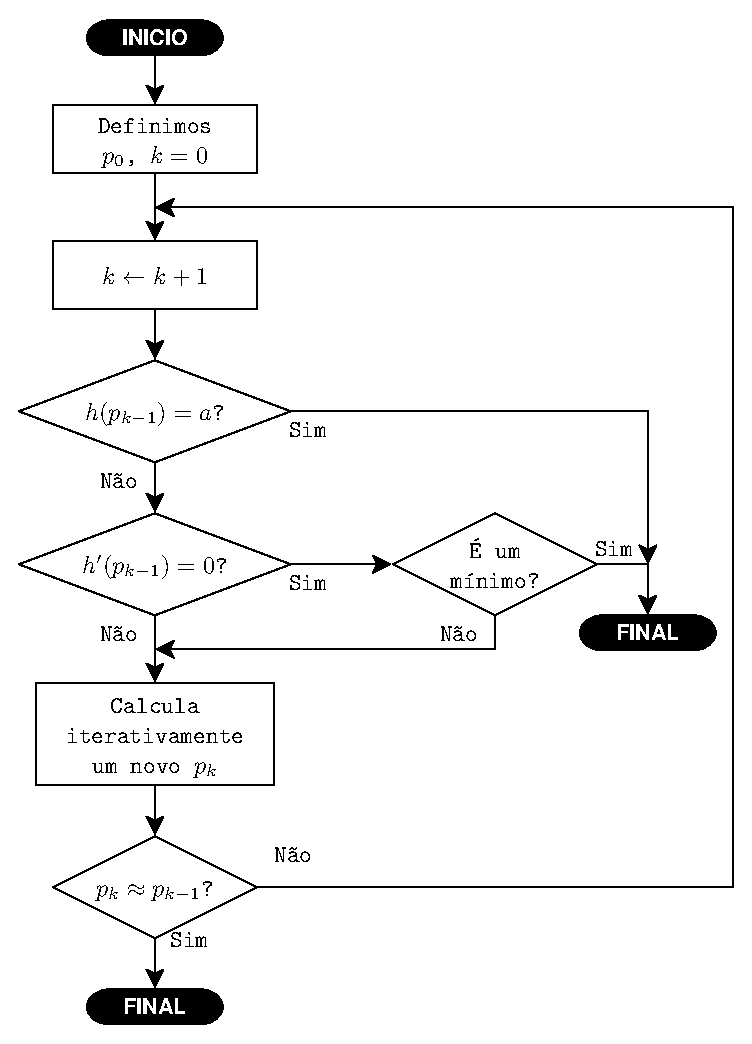
\includegraphics[width=0.75\textwidth]{chapters/minimization-hx/fluxo3.eps}
        \caption{Diagrama de fluxo da solução iterativa para achar um mínimo, seguindo a Prova \ref{proof:theo:minhxhxaxoxo}.}
        \label{fig:fluxohx3}
\end{figure}


\section{Provas dos teoremas}
 
%%%%%%%%%%%%%%%%%%%%%%%%%%%%%%%%%%%%%%%%%%%%%%%%%%%%%%%%%%%%%%%%%%%%%%%%%%%%%%%%%%%%%%%
%%%%%%%%%%%%%%%%%%%%%%%%%%%%%%%%%%%%%%%%%%%%%%%%%%%%%%%%%%%%%%%%%%%%%%%%%%%%%%%%%%%%%%%
\begin{myproofT}[Prova do Teorema \ref{theo:minhxhx}]\label{proof:theo:minhxhx}
Dados,
um escalar $x \in \mathbb{R}$, 
um escalar $a \in \mathbb{R}$,  
uma função $h:\mathbb{R} \rightarrow \mathbb{R}$, e 
definida a Eq. (\ref{eq:proof:minhxhx0}),
\begin{equation}\label{eq:proof:minhxhx0}
e(x)=||h(x)-a||^2.
\end{equation}
Para achar o valor  $\hat{x}$ que gere o menor valor de $e(x)$, é aplicado
o critério que um ponto de inflexão $x^+$ (máximo, mínimo ou ponto de sela) de $e(x)$ 
pode ser achado quando 
$\left. \frac{d e(x)}{d x }\right|_{x=x^+} \equiv e'(x^+) =0$.
Assim, 
usando o Teorema \ref{theo:derfxbCfxb0} podemos 
rescrever esta igualdade como a Eq. (\ref{eq:proof:minhxhxe}),
\begin{equation}\label{eq:proof:minhxhxe}
2  h'(x) \left[h(x) -a\right] = e'(x)=0,
\end{equation}
Da Eq. (\ref{eq:proof:minhxhxe}), observamos 
que existem duas formas de achar um ponto de inflexão $x^+$,
\begin{itemize}
 \item a primeira forma a achamos se temos um valor $x^+$ tal que $h'(x^+)=0$, 
que representa um ponto de inflexão simultâneo em $e(x)$ e $h(x)$, e
 \item a segunda forma é achando um valor $x^+$ tal que $h(x^+)=a$;
que representa um ponto de inflexão de $e(x)$, mas não
necessariamente de $h(x)$; 
sendo este ponto $x^+=\hat{x}$ também um mínimo absoluto, pois provocam $e(\hat{x})=0$.
\end{itemize}




Por outro lado, podemos realizar uma aproximação linear de $h(x)$ em $e(x)$
ao redor do ponto $p$, usando a \hyperref[def:taylor]{\textbf{serie de Taylor}},
de modo que a Eq. (\ref{eq:proof:minhxhx0}) pode ficar expressada como
\begin{equation}\label{eq:proof:minhxhxe:approx0}
e(x) \approx  e_p(x) = ||h'(p)\{x-p\}-\{a-h(p)\}||^2.
\end{equation}
Assim, da Eq. (\ref{eq:proof:minhxhxe:approx0})
podemos concluir que um ponto $x^*$ que é 
um mínimo da aproximação linear $e_p(x)$ feita em $e(x)$ ao redor do ponto $p$,
pode ser achado como
\begin{equation}\label{eq:proof:minhxhx2}
 h'(p)\{x^*-p\} = \{a-h(p)\} \qquad \leftrightarrow \qquad x^* = p - \frac{h(p)-a}{ h'(p)}.
\end{equation} 

Desta equação podemos tirar a seguintes conclusões:
\begin{itemize}

\item Observamos que a posição $p$ é corregida para ficar próximo à posição $x^*$, 
que é um mínimo absoluto de $e_p(x)$ na direção de um mínimo (qualquer) de $e(x)$;
pelo que se deduz que a Eq. (\ref{eq:proof:minhxhx2})
pode ser usada para procurar aproximações $x^*$ de pontos mínimos $\hat{x}$ em $e(x)$ desde a posição $p$;
ou pelo menos aproximações de novas posições em caminhos numa direção descendente de $e(x)$.

\item A Eq. (\ref{eq:proof:minhxhx2}) é satisfeita 
com $x^* \approx p$ se acharmos um  
ponto $p$ onde  $a \approx h(p)$; 
é dizer um mínimo global de $e(x)$ em $p$.%, como pode ser visto na Figura \ref{fig:ex0a}. 

\item Dado que a Eq. (\ref{eq:proof:minhxhx2}) tem um termo $h'(p)$ no denominador,
valores $p$ que cumpram $h'(p)\approx 0$ provocam uma correção distante (divergência) da posição $p$,
nos casos onde $p$ se aproxime a máximos e pontos de sela,
ou mínimos locais. 
Mas sim se trata de um mínimo global com $h(p)\approx a$, 
o comportamento será inesperado e dependerá se é finito ou não, o
\begin{equation}
lim_{x\rightarrow p } \frac{h(p)-a}{h'(p)}.
\end{equation}

\item Se modificamos a Eq. (\ref{eq:proof:minhxhx2}), e escolhemos um ponto  
$p_0$ que consideremos próximo ao ponto $\hat{x}$ que minimiza $e(\hat{x})$,
podemos achar iterativamente aproximações lineares $x^*$ cada vez mais próximos a  $\hat{x}$,
se usamos a seguinte equação iterativa,
\begin{equation}\label{eq:proof:minhxhx3}
p_{k} \leftarrow p_{k-1} - \frac{ h(p_{k-1})-a}{h'(p_{k-1})},
\end{equation}
iniciando desde um $p_{0}$ 
ate que exista uma tendencia prolongada onde se observe que $p_{k}$ é muito próximo a $p_{k-1}$,
momento no qual declaramos que $\hat{x} \approx p_{k}$.
\item Pode existir um mínimo global $\hat{x}$ de $e(\hat{x})>0$.
Isto nos restringe a que no uso da Eq. (\ref{eq:proof:minhxhx3}),
nosso critério principal para estabelecer o final do cáculo iterativo,
deve ser a tendencia na  proximidade entre $p_{k}$ e $p_{k-1}$ 
e não o valor de $e(x_k)$.
\end{itemize}

Um diagrama completo resumindo todas estas conclusões pode ser visto na Figura \ref{fig:fluxohx1}.
\end{myproofT}



\begin{figure}[!h]
     \centering
         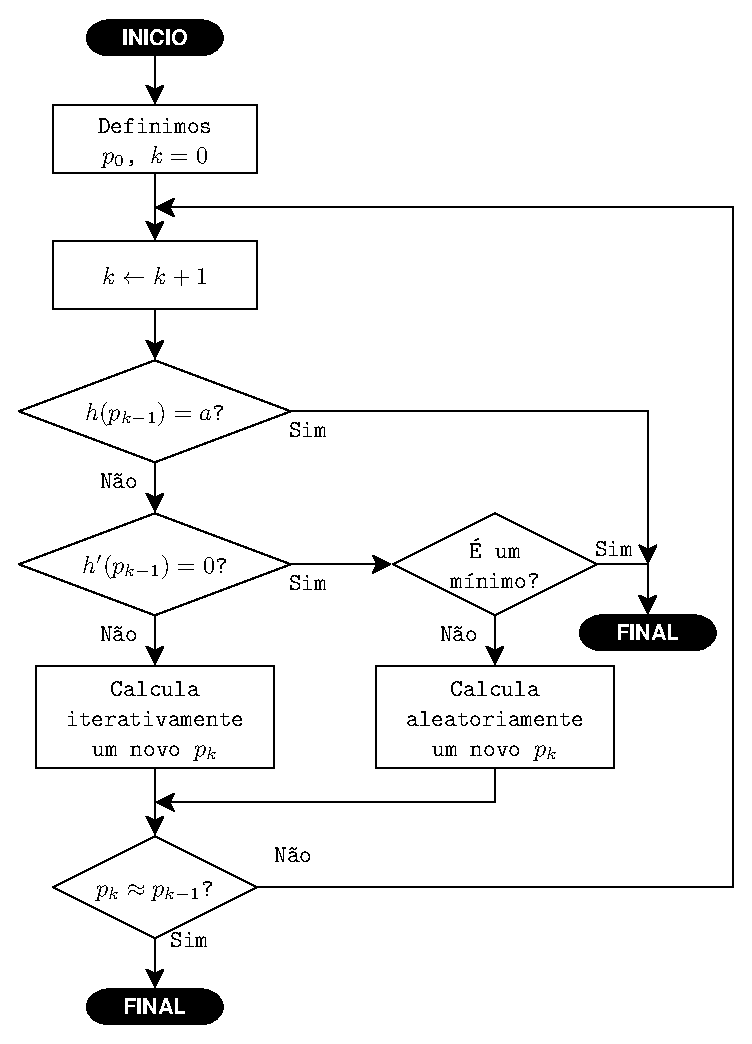
\includegraphics[width=0.75\textwidth]{chapters/minimization-hx/fluxo1.eps}
        \caption{Diagrama de fluxo da solução iterativa para achar um mínimo, seguindo a Prova \ref{proof:theo:minhxhx}.}
        \label{fig:fluxohx1}
\end{figure}


%%%%%%%%%%%%%%%%%%%%%%%%%%%%%%%%%%%%%%%%%%%%%%%%%%%%%%%%%%%%%%%%%%%%%%%%%%%%%%%%%%%%%%%
%%%%%%%%%%%%%%%%%%%%%%%%%%%%%%%%%%%%%%%%%%%%%%%%%%%%%%%%%%%%%%%%%%%%%%%%%%%%%%%%%%%%%%%
\begin{myproofT}[Prova do Teorema \ref{theo:minhxhxxbxb}]\label{proof:theo:minhxhxxbxb}

Dados,
um escalar $x \in \mathbb{R}$, 
um escalar $a \in \mathbb{R}$,
um escalar $\alpha \in \mathbb{R}^{+}$,
um escalar $b \in \mathbb{R}$,
uma função $h:\mathbb{R} \rightarrow \mathbb{R}$, e 
definida a Eq. (\ref{eq:proof:minhxhxxbxb0}),
\begin{equation}\label{eq:proof:minhxhxxbxb0}
e(x)=||h(x)-a||^2+\alpha ||x-b||^2.
\end{equation}

Para achar o valor  $\hat{x}$ que gere o menor valor de $e(x)$, é aplicado
o critério que um ponto de inflexão $x^+$ (máximo, mínimo ou ponto de sela) de $e(x)$ 
pode ser achado quando 
$\left. \frac{d e(x)}{d x }\right|_{x=x^+} \equiv e'(x^+) =0$.
Assim, 
usando o Teorema \ref{theo:derfxbCfxb0} e \ref{theo:derAxbAxb}  podemos 
rescrever esta igualdade como a Eq. (\ref{eq:proof:minhxhxxbxbe}),
\begin{equation}\label{eq:proof:minhxhxxbxbe}
2  h'(x) \left[h(x) -a\right]+2\alpha (x-b)= e'(x)=0,
\end{equation}
Da Eq. (\ref{eq:proof:minhxhxxbxbe}), observamos 
que existem duas formas de achar um ponto de inflexão $x^+$,
\begin{itemize}
 \item a primeira forma a achamos se temos um valor $x^+=b$ tal que $h'(b)=0$, 
que representa um ponto de inflexão simultâneo em $e(x)$ e $h(x)$, e
 \item a segunda forma é achando um valor $x^+=b$ tal que $h(b)=a$;
que representa um ponto de inflexão de $e(x)$, mas não
necessariamente de $h(x)$; 
sendo este ponto $x^+=\hat{x}=b$ também um mínimo absoluto, pois provocam $e(\hat{x})=0$.
\end{itemize}

Por outro lado, podemos realizar uma aproximação linear de $h(x)$ em $e(x)$
ao redor do ponto $p$, usando a \hyperref[def:taylor]{\textbf{serie de Taylor}},
de modo que a Eq. (\ref{eq:proof:minhxhxxbxb0}) pode ficar expressada como
\begin{equation}\label{eq:proof:minhxhxxbxbe:approx0}
e(x) \approx  e_p(x) = ||h'(p)\{x-p\}-\{a-h(p)\}||^2+\alpha ||x-b||^2.
\end{equation}
Assim, da Eq. (\ref{eq:proof:minhxhxxbxbe:approx0})
podemos concluir que um ponto $x^*$ que é 
o mínimo da aproximação linear $e_p(x)$ feita em $e(x)$ ao redor do ponto $p$,
pode ser achado aplicando $\left. \frac{d e_p(x)}{d x }\right|_{x=x^*} \equiv e_{p}'(x^*) =0$,
de modo que obtemos
\begin{equation}\label{eq:proof:minhxhxaxb2a}
 2 h'(p)[h'(p)\{x^*-p\} -\{a-h(p)\}] + \alpha [x^*-b] = 0,
\end{equation} 
\begin{equation}\label{eq:proof:minhxhxaxb2}
x^* = p - \frac{h'(p)\{h(p)-a\}+\alpha\{p-b\}}{ h'(p)^2+\alpha}.
\end{equation} 

Desta equação podemos tirar a seguintes conclusões:


\begin{itemize}

\item Observamos que a posição $p$ é corregida para ficar próximo à posição $x^*$, 
que é um mínimo absoluto de $e_p(x)$ na direção de um mínimo (qualquer) de $e(x)$;
pelo que se deduz que a Eq. (\ref{eq:proof:minhxhxaxb2})
pode ser usada para procurar aproximações $x^*$ de pontos mínimos $\hat{x}$ em $e(x)$ desde a posição $p$;
ou pelo menos aproximações de novas posições em caminhos numa direção descendente de $e(x)$.

\begin{comment}
\item A Eq. (\ref{eq:proof:minhxhxaxb2}) é satisfeita 
com $x^* \approx p$ se acharmos um  
ponto $p=b$ onde  $a \approx h(b)$; 
é dizer um mínimo global de $e(x)$ em $b$.%, como pode ser visto na Figura \ref{fig:ex0a}. 
\item A Eq. (\ref{eq:proof:minhxhxaxb2}) é satisfeita 
com $x^* \approx p$ se acharmos um  
ponto $p=b$ onde  $0 \approx h'(b)$; 
é dizer um ponto de inflexão de $e(x)$ em $b$.
\end{comment}

\item Se reescrevemos a Eq. (\ref{eq:proof:minhxhxaxb2}) usando o Teorema \ref{theo:derfxbCfxb0}
e o Corolário \ref{coro:derAxbAxb2},
obtemos
\begin{equation}\label{eq:proof:minhxhxaxbea1}
x^* \approx p -
\frac{ e'(p)}{2 \{h'(p)^2+\alpha\} },
\end{equation}
onde a Eq. (\ref{eq:proof:minhxhxaxbea1}) é satisfeita 
com $x^* \approx p$
se acharmos um  ponto $p$ onde  
$e'(p)\approx 0$; 
é dizer $p$ é um ponto de inflexão de $e(x)$, como já foi analisado na Eq. (\ref{eq:proof:minhxhxxbxbe}).
%como pode ser visto na Figura \ref{fig:ex0b}.
Porem, dado que a Eq. (\ref{eq:proof:minhxhxaxbea1}) avança desde $p$ na direção de um mínimo $x^*$, 
mesmo que nos pontos de inflexão correspondentes a máximos ou pontos de sela,
encontremos valores de $p$ próximos a $x^*$,
 estes casos serão pouco estáveis pois
a correção da posição $p$ será na direção de um mínimo e não do máximo.

\item Se modificamos a Eq. (\ref{eq:proof:minhxhxaxb2}), e escolhemos um ponto  
$p_0$ que consideremos próximo ao ponto $\hat{x}$ que minimiza $e(\hat{x})$,
podemos achar iterativamente aproximações lineares $x^*$ cada vez mais próximos a  $\hat{x}$,
se usamos a seguinte equação iterativa,
\begin{equation}\label{eq:proof:minhxhxaxb3}
p_{k} \leftarrow p_{k-1} - \frac{ h'(p_{k-1})\{h(p_{k-1})-a\}+\alpha\{p-b\}}{h'(p_{k-1})^2+\alpha},
\end{equation}
iniciando desde um $p_{0}$ 
ate que exista uma tendencia prolongada onde se observe que $p_{k}$ é muito próximo a $p_{k-1}$,
momento no qual declaramos que $\hat{x} \approx p_{k}$.
\item Pode existir um mínimo global $\hat{x}$ de $e(\hat{x})>0$.
Isto nos restringe a que no uso da Eq. (\ref{eq:proof:minhxhxaxb3}),
nosso critério principal para estabelecer o final do cáculo iterativo,
deve ser a tendencia na  proximidade entre $p_{k}$ e $p_{k-1}$ 
e não o valor de $e(x_k)$.
\end{itemize}

Um diagrama completo resumindo todas estas conclusões pode ser visto na Figura \ref{fig:fluxohx2}.
\end{myproofT}



\begin{figure}[!h]
     \centering
         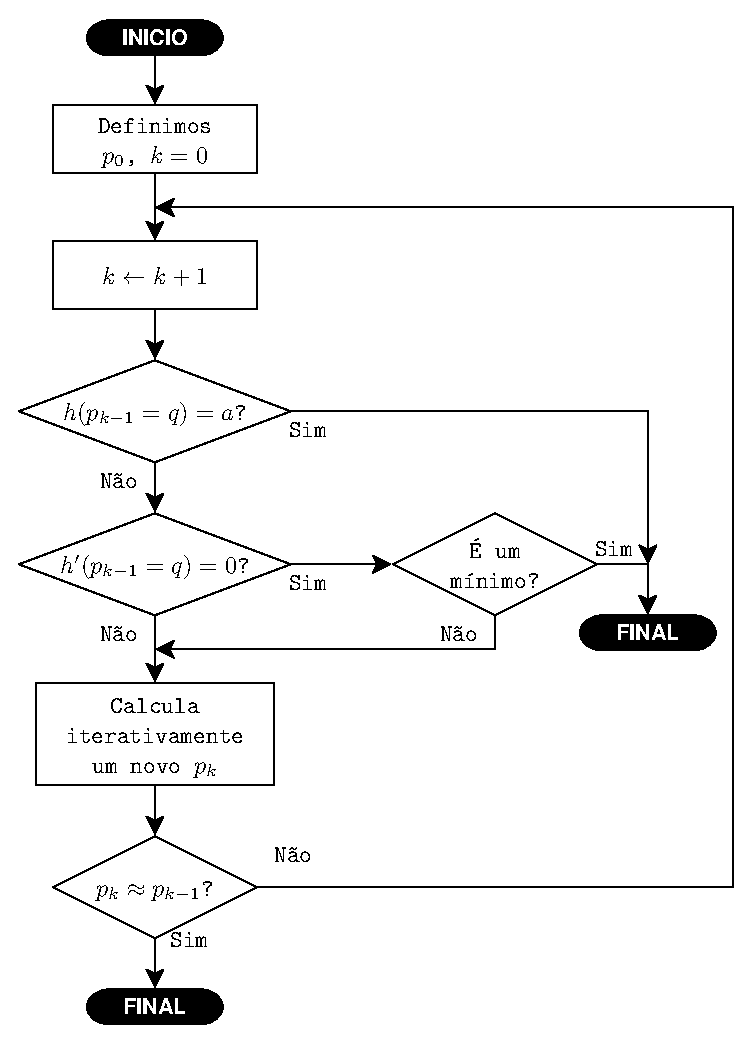
\includegraphics[width=0.75\textwidth]{chapters/minimization-hx/fluxo2.eps}
        \caption{Diagrama de fluxo da solução iterativa para achar um mínimo, seguindo a Prova \ref{proof:theo:minhxhxxbxb}.}
        \label{fig:fluxohx2}
\end{figure}


%%%%%%%%%%%%%%%%%%%%%%%%%%%%%%%%%%%%%%%%%%%%%%%%%%%%%%%%%%%%%%%%%%%%%%%%%%%%%%%%%%%%%%%
%%%%%%%%%%%%%%%%%%%%%%%%%%%%%%%%%%%%%%%%%%%%%%%%%%%%%%%%%%%%%%%%%%%%%%%%%%%%%%%%%%%%%%%
\begin{myproofT}[Prova do Teorema \ref{theo:minhxhxxoxo}]\label{proof:theo:minhxhxaxoxo}

Dados,
um escalar $x \in \mathbb{R}$, 
um escalar $a \in \mathbb{R}$,
um escalar $\alpha \in \mathbb{R}^{+}$,
um escalar $x_{last} \in \mathbb{R}$,
uma função $h:\mathbb{R} \rightarrow \mathbb{R}$, e 
definida a Eq. (\ref{eq:proof:minhxhxxoxo0}),
\begin{equation}\label{eq:proof:minhxhxxoxo0}
e(x)=||h(x)-a||^2+\alpha ||x-x_{last}||^2.
\end{equation}
tendo em consideração que $x_{last}$ é uma constante equivalente a $x_{k-1}$
numa busca iterativa ou equivalente a $p$, 
se decidimos usar uma aproximação linear ao redor de $p$ em $h(x)$; 
é dizer, o segundo somando na Eq. (\ref{eq:proof:minhxhxxoxo0}) 
procura minimizar $||x_{k}-x_{k-1}||^2$.


Para achar o valor  $\hat{x}$ que gere o menor valor de $e(x)$, é aplicado
o critério que um ponto de inflexão $x^+$ (máximo, mínimo ou ponto de sela) de $e(x)$ 
pode ser achado quando 
$\left. \frac{d e(x)}{d x }\right|_{x=x^+} \equiv e'(x^+) =0$.
Assim, 
usando o Teorema \ref{theo:derfxbCfxb0} e \ref{theo:derAxbAxb}  podemos 
rescrever esta igualdade como a Eq. (\ref{eq:proof:minhxhxxoxoe}),
\begin{equation}\label{eq:proof:minhxhxxoxoe}
2  h'(x) \left[h(x) -a\right]+2\alpha (x-x_{last})= e'(x)=0,
\end{equation}
Da Eq. (\ref{eq:proof:minhxhxxoxoe}), observamos 
que existem duas formas de achar um ponto de inflexão $x^+$,
\begin{itemize}
 \item a primeira forma a achamos se temos um valor $x^+=x_{last}$ tal que $h'(x_{last})=0$, 
que representa um ponto de inflexão simultâneo em $e(x)$ e $h(x)$, e
 \item a segunda forma é achando um valor $x^+=x_{last}$ tal que $h(x_{last})=a$;
que representa um ponto de inflexão de $e(x)$, mas não
necessariamente de $h(x)$; 
sendo este ponto $x^+=\hat{x}=x_{last}$ também um mínimo absoluto, pois provocam $e(\hat{x})=0$.
\end{itemize}

Por outro lado, procurando outros critérios para achar os pontos de inflexão,
podemos igualar $x_{last}\equiv p$ e 
realizar uma aproximação linear de $h(x)$ em $e(x)$
ao redor do ponto $p$ usando a \hyperref[def:taylor]{\textbf{serie de Taylor}},
de modo que a Eq. (\ref{eq:proof:minhxhxxoxo0}) pode ficar expressada como
\begin{equation}\label{eq:proof:minhxhxxoxo0approx}
e(x) \approx e_{p}(x)  \equiv ||h'(p)[x-p]-[a-h(p)]||^2+\alpha||x-p||^2,
\end{equation}


%%%%%%%
Assim, usando o resultado da Prova \ref{proof:theo:minAxbCAxbalphaxqD} na Eq. (\ref{eq:proof:minhxhxxoxo0approx}), 
podemos concluir que um ponto $x^*$ que é 
o mínimo da aproximação linear $e_p(x)$ feita em $e(x)$ ao redor do ponto $p$,
pode ser achado aplicando $\left. \frac{d e_p(x)}{d x }\right|_{x=x^*} \equiv e_{p}'(x^*) =0$,
de modo que obtemos
\begin{equation}\label{eq:proof:minhxhxaxo2a}
 2 h'(p)[h'(p)\{x^*-p\} -\{a-h(p)\}] + \alpha [x^*-p] = 0,
\end{equation} 
\begin{equation}\label{eq:proof:minhxhxaxo2}
x^* = p - \frac{h'(p)\{h(p)-a\}}{ h'(p)^2+\alpha}.
\end{equation} 








Desta equação podemos tirar a seguintes conclusões:
\begin{itemize}

\item Observamos que a posição $p$ é corregida para ficar próximo à posição $x^*$, 
que é o valor mínimo na aproximação linear ao redor de $p$;
pelo que se deduz que a Eq. (\ref{eq:proof:minhxhxaxo2})
pode ser usada para procurar aproximações de pontos mínimos $\hat{x}$ em $e(x)$ desde a posição $p$,
ou pelo menos aproximações de novas posições em caminhos numa direção descendente de $e(x)$.

\begin{comment}
\item A Eq. (\ref{eq:proof:minhxhxaxo2}) é satisfeita 
com $x^* \approx p$ se acharmos um  
ponto $p$ onde  $a \approx h(p\approx x_{last})$; 
é dizer um mínimo global de $e(x)$ em $p$. 
\end{comment}

\item Se reescrevemos a Eq. (\ref{eq:proof:minhxhxaxo2}) usando o Teorema \ref{theo:derfxbCfxb0}
e o Corolário \ref{coro:derAxbAxb2},
obtemos
\begin{equation}\label{eq:proof:minhxhxaxoxo2ea1}
x^* \approx p - \frac{ e'(p)}{2(h'(p)^2+\alpha)},
\end{equation}
onde a Eq. (\ref{eq:proof:minhxhxaxoxo2ea1}) é satisfeita 
com $x^* \approx p$
se acharmos um  ponto $p$ onde  
$e'(p)\approx 0$; 
é dizer $p$ é um ponto de inflexão de $e(x)$, como pode ser visto na Eq. (\ref{eq:proof:minhxhxxoxoe}).
Porem, dado que a Eq. (\ref{eq:proof:minhxhxaxoxo2ea1}) avança desde $p$ na direção de um mínimo $x^*$, 
mesmo que nos pontos de inflexão correspondentes a máximos ou pontos de sela,
encontremos valores de $p$ próximos a $x^*$,
 estes casos serão pouco estáveis pois
a correção da posição $p$ será na direção de um mínimo e não do máximo.

\item Se modificamos a Eq. (\ref{eq:proof:minhxhxaxo2}), e escolhemos um ponto  
$p_0$ que consideremos próximo ao ponto $\hat{x}$ que minimiza $e(\hat{x})$,
podemos achar iterativamente aproximações lineares $x^*$ cada vez mais próximos a  $\hat{x}$,
se usamos a seguinte equação iterativa,
\begin{equation}\label{eq:proof:minhxhxaxoxo3b}
p_{k} \leftarrow p_{k-1} - \frac{h'(p_{k-1})\{h(p_{k-1})-a\}}{h'(p_{k-1})^2 +\alpha},
\end{equation}
onde se inicia desde um $p_{0}$ 
ate que exista uma tendencia prolongada onde se observe que $p_{k}$ é muito próximo a $p_{k-1}$,
momento no qual declaramos que $\hat{x} \approx p_{k}$.
Disto também se deduz que o erro a minimizar em cada iteração será diferente e influenciado pelo valor do ponto $p_{k-1}$,
\begin{equation}
e_{k-1}(x)  \equiv ||h(x)-a||^2+\alpha||x-p_{k-1}||^2
\end{equation}
\item Pode existir um mínimo global $\hat{x}$ de $e(\hat{x}) > 0$.
Isto nos restringe a que no uso da Eq. (\ref{eq:proof:minhxhxaxoxo3b}),
nosso critério principal para estabelecer o final do cáculo iterativo,
deve ser a tendencia na  proximidade entre $p_{k}$ e $p_{k-1}$ 
e não o valor de $e(x_k)$.
\end{itemize}~

Um diagrama completo resumindo todas estas conclusões pode ser visto na Figura \ref{fig:fluxohx3}.
\end{myproofT}
\begin{figure}[!h]
     \centering
         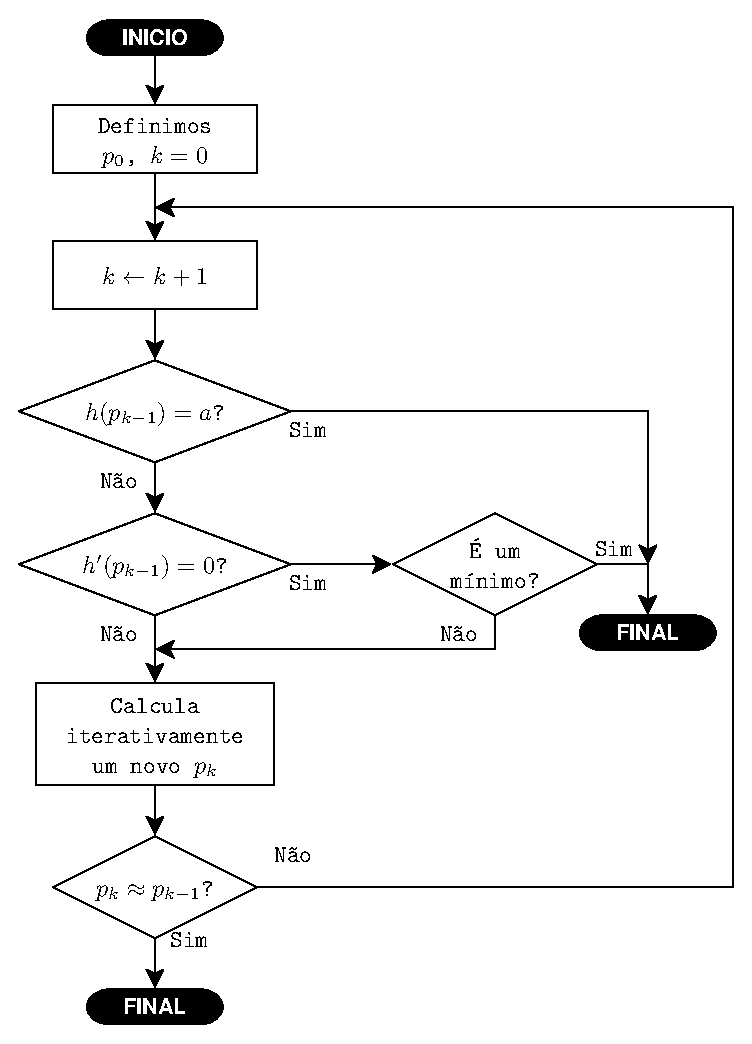
\includegraphics[width=0.75\textwidth]{chapters/minimization-hx/fluxo3.eps}
        \caption{Diagrama de fluxo da solução iterativa para achar um mínimo, seguindo a Prova \ref{proof:theo:minhxhxaxoxo}.}
        \label{fig:fluxohx3}
\end{figure}


%----------------------------------------------------------------------------------------
%	PART
%----------------------------------------------------------------------------------------
\part{Problemas de achar raízes de funções}
%----------------------------------------------------------------------------------------
%	CHAPTER  
%----------------------------------------------------------------------------------------
\chapterimage{chapter_roots.pdf} % Chapter heading image

\chapter{Raízes de funções}


%%%%%%%%%%%%%%%%%%%%%%%%%%%%%%%%%%%%%%%%%%%%%%%%%%%%%%%%%%%%%%%%%%%%%%%%%%%%%%%%%%%%%%%
\section{ Método de Newton para funções $h(x)$: $\mathbb{R}$ $\rightarrow$ $\mathbb{R}$ }

\begin{theorem}[Solução iterativa]\label{theo:rootshx}
~\\
\begin{minipage}{0.20\textwidth}
\centering
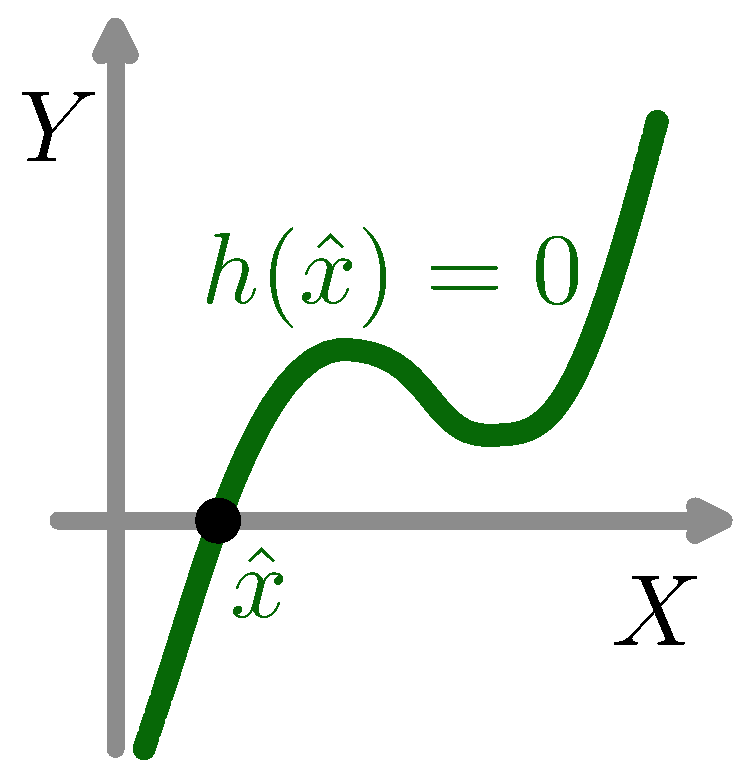
\includegraphics[width=0.9\linewidth]{chapters/roots/roots1.eps} 
\end{minipage}
\begin{minipage}{0.8\textwidth}
Dados,
um escalar $\delta \in \mathbb{R}_+$, 
um escalar $x \in \mathbb{R}$, 
uma função $h:\mathbb{R} \rightarrow \mathbb{R}$, e 
conhecida a validade da Eq. (\ref{eq:rootshx1}),
\begin{equation}\label{eq:rootshx1}
0=h(x);
\end{equation}
se desejamos ter o valor $x=\hat{x}$ que cumpra a Eq. (\ref{eq:rootshx1}),
podemos usar iterativamente a Eq. (\ref{eq:rootshx2}),
onde  $h'(x)\equiv \frac{d h(x)}{d x}$,
\end{minipage}

\begin{equation}\label{eq:rootshx2}
x_{k} \leftarrow x_{k-1}-\frac{ h(x_{k-1})}{h'(x_{k-1})}.
\end{equation}
Assim, $\hat{x}$ pode ser achado\footnote{A 
demostração pode ser vista na Prova \ref{proof:theo:rootshx}.} 
iniciando a Eq. (\ref{eq:rootshx2}) desde um 
$x_{0}$ qualquer, realizando cálculos $x_{k}$ iterativamente  
ate\footnote{Sendo $\delta$ um valor pequeno próximo a zero.} que $||h(x_k)||<\delta$
onde se declara que $\hat{x}=x_k$.

\textbf{Considerações:}
\begin{itemize} 
\item Se $h'(x_{k-1})\approx 0$, então estamos perto de um ponto de inflexão 
(máximo, mínimo ou ponto de sela) em $x_{k-1}$. Nestos pontos a Eq. (\ref{eq:rootshx2}): 
\begin{itemize}
\item Diverge quando se cumpre que $h(x_{k-1})\neq 0$, ou
\item Converge\footnote{A demostração pode ser vista na Prova \ref{proof:theo:cont:rootshx}.} 
se $h(x_{k-1}) = 0$ e se verifica que $h(x)$ pode ser representado 
mediante uma \hyperref[def:taylor]{\textbf{série de Taylor}} ao redor de $x_{k-1}$, 
 pois indica que $\lim_{x\rightarrow x_{k-1}}  h(x)/h'(x)$ é finito.
\end{itemize}
\item Uma sugestão do procedimento para a busca de uma raiz pode ser vista no diagrama de fluxo
mostrado na Figura \ref{fig:fluxorhx1}. 
\end{itemize}
\end{theorem}

\begin{figure}[!h]
     \centering
         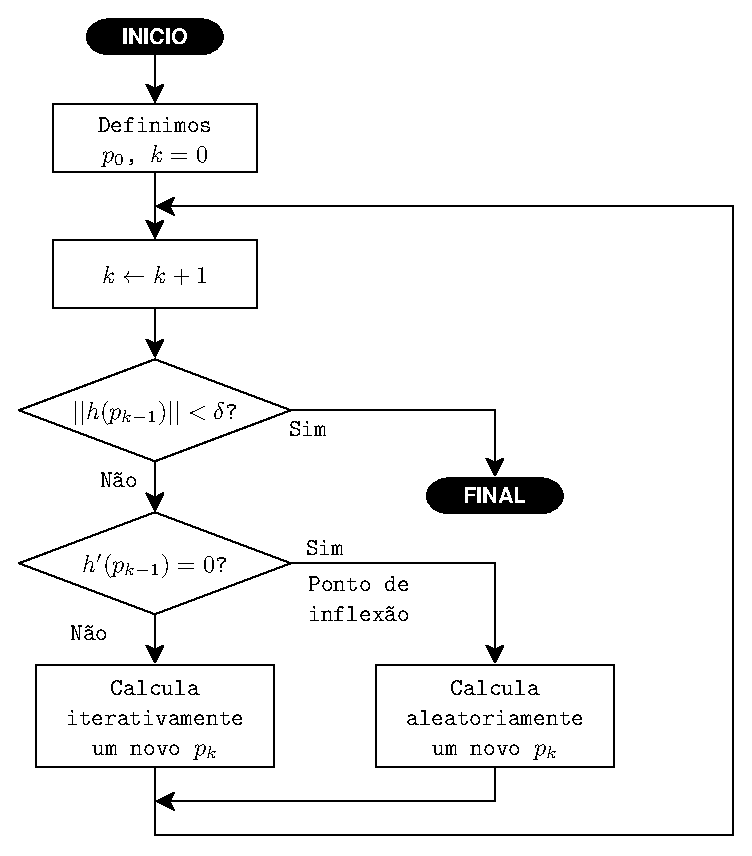
\includegraphics[width=0.75\textwidth]{chapters/roots/fluxo1.eps}
        \caption{Diagrama de fluxo da solução iterativa para achar uma raiz, seguindo o teorema \ref{theo:rootshx}.}
        \label{fig:fluxorhx1}
\end{figure}

\newpage
%%%%%%%%%%%%%%%%%%%%%%%%%%%%%%%%%%%%%%%%%%%%%%%%%%%%%%%%%%%%%%%%%%%%%%%%%%%%%%%%
\subsection{Exemplos de busca de raízes pelo método de Newton}


\begin{example}\label{ex:rootshx1}
Conhecida uma função $h(x)=x(x^2-1)+1$, e um escalar $\delta=10^{-3}$;
usando o Teorema \ref{theo:rootshx}, 
achar um valor $x=\hat{x}$ que cumpra $||h(x)||<\delta$.
Podemos ver as respostas a este exemplo na Solução \ref{sol:rootshx1} e \ref{sol:rootshx2}.
\end{example}
\begin{SolutionT}[Relativa ao Exemplo \ref{ex:rootshx1} (Diverge):]\label{sol:rootshx1}
 A Fig. \ref{fig:rootsNcasesa} nos mostra o processo de busca das raízes de $h(x)$. 
A busca inicia em $x_0=-0.3$, 
todos os valores $x_{k}$ podem ser vistos na
Tabela \ref{tab:rootsNcases1}. 
Neste caso a busca iterativa indicada pela Eq. (\ref{eq:rootshx2}) 
diverge para valores próximos a $x_m=\frac{\sqrt{3}}{3}\approx 0.57735$,
que é um mínimo local de $h(x)$; é dizer $h'(x_m)\approx 0$ e $h(x_m)\neq 0$.
É fácil de observar, que neste caso se produz 
uma especie de efeito sanfona, onde $x_{k}$ se aproxima ao mínimo local em $h(x)$, e quando 
está próximo deste valor a busca volta divergir a um ponto medianamente distante.
\end{SolutionT}

\begin{figure}[!h]
    \centering
    \begin{subfigure}[b]{0.49\textwidth}
        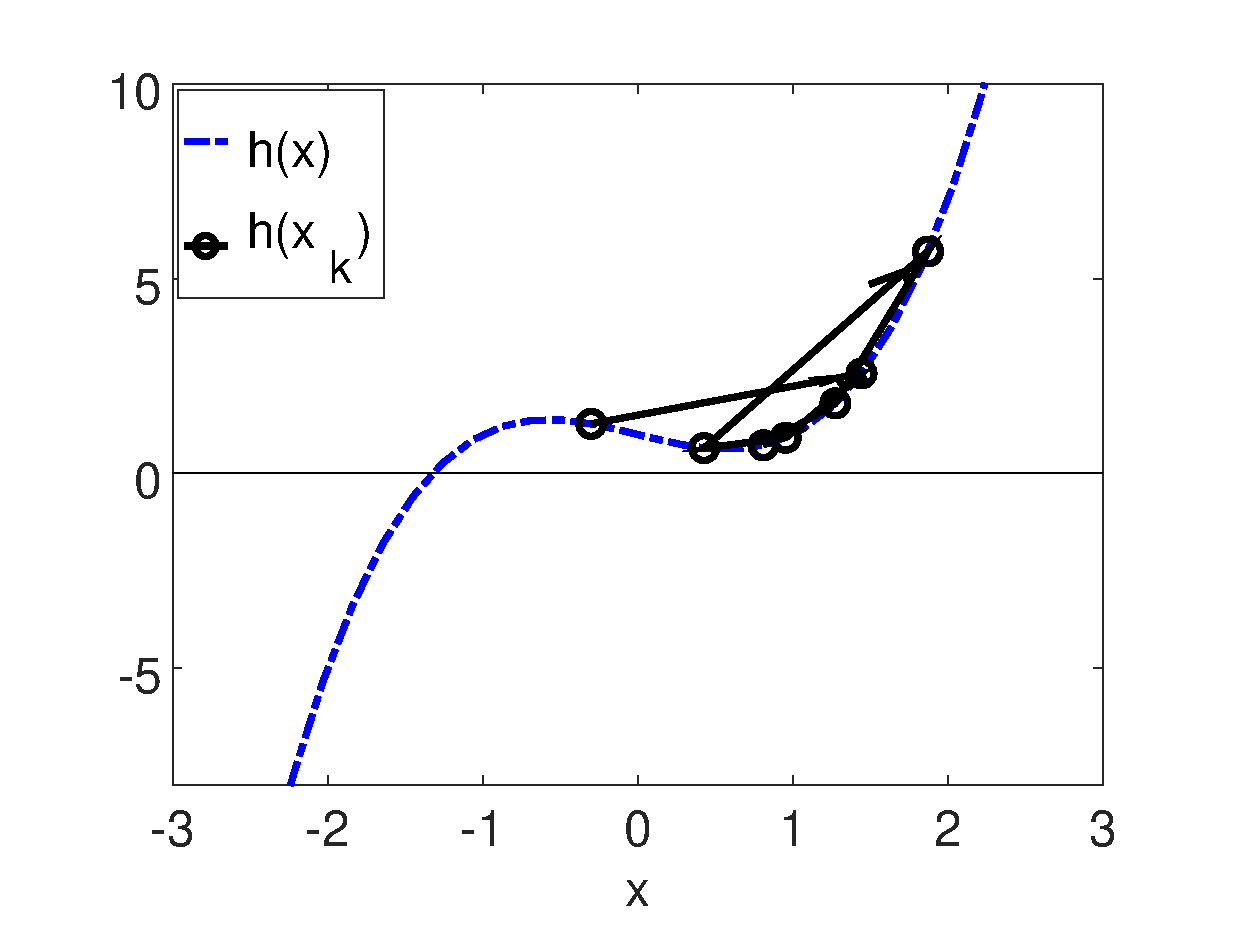
\includegraphics[width=\textwidth]{chapters/roots/mfiles/hx/minimizando_hx_1.eps}
        \caption{As iterações divergem ao redor de $x_m$, onde $h'(x_m)\approx 0$ e $h(x_m)\neq 0$.}
        \label{fig:rootsNcasesa}
    \end{subfigure}
    ~ %add desired spacing between images, e. g. ~, \quad, \qquad, \hfill etc. 
      %(or a blank line to force the subfigure onto a new line)
    \begin{subfigure}[b]{0.49\textwidth}
        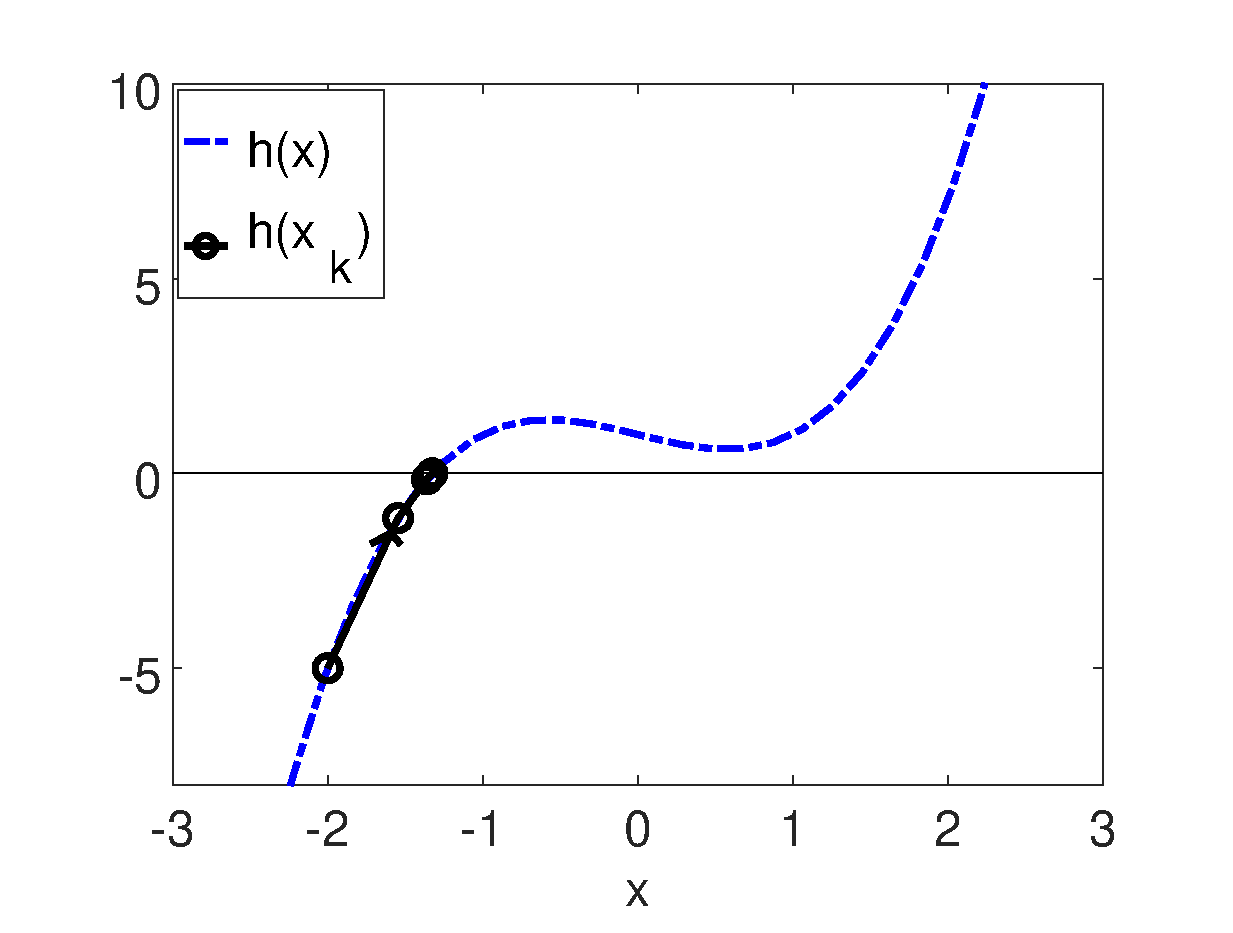
\includegraphics[width=\textwidth]{chapters/roots/mfiles/hx/minimizando_hx_2.eps}
        \caption{As iterações convergem em $\hat{x}$, onde $h(\hat{x})\approx 0$ e $h'(x_m)\neq 0$}
        \label{fig:rootsNcasesb}
    \end{subfigure}
    \caption{Comportamento da busca iterativa do Exemplo \ref{ex:rootshx1}}
    \label{fig:rootsNcases}
\end{figure}

\begin{table}[!h]
\centering
\begin{tabular}{|l|l|l|l|l|l|l|l|}
\hline
$k$      & 0 & 1 & 2 & 3 & 4 & 5 & 6\\ \hline
$x_k$    & -0.30000 & 1.44384 & 0.95543 & 0.42813 & 1.87298 & 1.27476 & 0.81109 \\ \hline
$||h(x_k)||$ & 1.27300 & 2.56607 & 0.91673 & 0.65034 & 5.69758 & 1.79676 & 0.72250 \\ \hline
\end{tabular}
\caption{Resposta iterativa do Exemplo \ref{ex:rootshx1}.}
\label{tab:rootsNcases1}
\end{table}

\begin{SolutionT}[Relativa ao Exemplo \ref{ex:rootshx1} (Converge):]\label{sol:rootshx2}
A Fig. \ref{fig:rootsNcasesb} nos mostra o processo de busca de uma raiz de $h(x)$. 
A busca inicia em $x_0=-2.0$,
 todos os valores $x_{k}$ podem ser vistos na Tabela \ref{tab:rootsNcases2}. 
Neste caso a busca iterativa indicada pela Eq. (\ref{eq:rootshx2}) converge 
em $x_4\approx 0$ com $||h(x_4)||<\delta$ que corresponde a uma raiz de $h(x)$.
\end{SolutionT}

\begin{table}[!h]
\centering
\begin{tabular}{|l|l|l|l|l|l|}
\hline
$k$      & 0 & 1 & 2 & 3 & 4 \\ \hline
$x_k$    & -2.0000 & -1.5455 & -1.3596 & -1.3258 & -1.3247 \\ \hline
$||h(x_k)||$ & 5.0000 &  1.1458 & 1.5370e-01 & 4.6249e-03 & 4.6577e-06 \\ \hline
\end{tabular}
\caption{Resposta iterativa do Exemplo \ref{ex:rootshx1}.}
\label{tab:rootsNcases2}
\end{table}

\begin{example}\label{ex:rootshx2}
Conhecida uma função $h(x)=x(x^2-1)+2\frac{\sqrt{3}}{9}$, e um escalar $\delta=2~10^{-5}$;
usando o Teorema \ref{theo:rootshx},
achar o valor $x=\hat{x}$ que cumpra $||h(x)||<\delta$.
Podemos ver a resposta a este exemplo na Solução \ref{sol:rootshx3}.
\end{example}

\begin{SolutionT}[Relativa ao Exemplo \ref{ex:rootshx2} (Converge):]\label{sol:rootshx3}
A Fig. \ref{fig:rootsNcasesc} nos mostra o processo de busca de uma raiz de $h(x)$. 
A busca inicia em $x_0=-0.3$,
 todos os valores $x_{k}$ podem ser vistos na Tabela \ref{tab:rootsNcases3}. 
Neste caso a busca iterativa indicada pela Eq. (\ref{eq:rootshx2}) converge 
em $x_4\approx 0$ com $||h(x_4)||<\delta$ que corresponde a uma raiz de $h(x)$.
Analiticamente podemos verificar que uma raiz pode ser achada em $x_m=\frac{\sqrt{3}}{3}\approx 0.57735$.
\end{SolutionT}

\begin{table}[!h]
\centering
\begin{tabular}{|l|l|l|l|l|l|}
\hline
$k$      & 0 & 1 & 2 & 3 & 4 \\ \hline
$x_k$    & -0.30000 & 0.60123 & 0.58937 & 0.58338 & 0.58037 \\ \hline
$||h(x_k)||$ & 6.5790e-01 & 1.0016e-03 & 2.5207e-04 & 6.3234e-05 & 1.5836e-05 \\ \hline
\end{tabular}
\caption{Resposta iterativa do Exemplo \ref{ex:rootshx1}.}
\label{tab:rootsNcases3}
\end{table}

    \begin{figure}[!h]
        \centering
        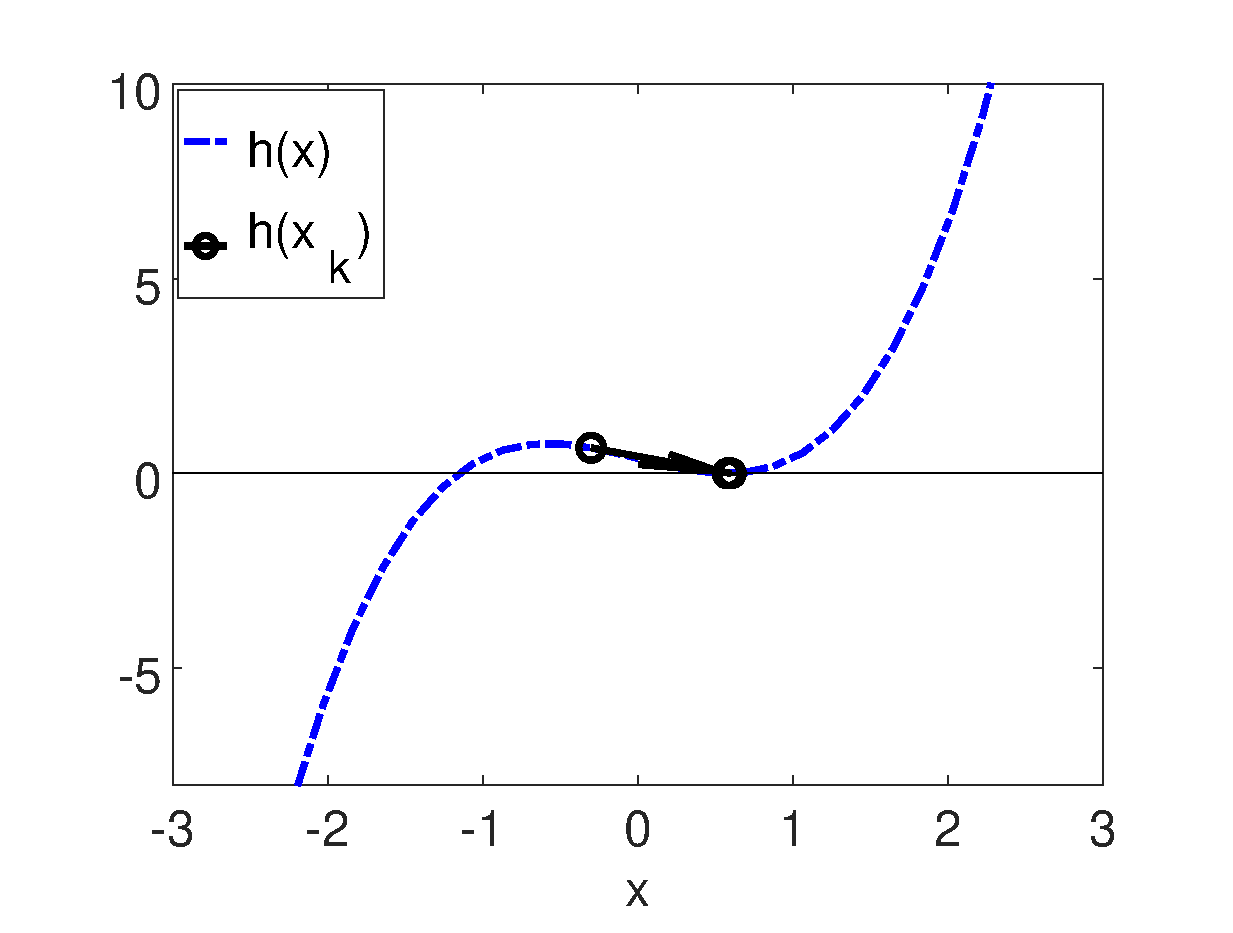
\includegraphics[width=0.49\textwidth]{chapters/roots/mfiles/hx2/minimizando_hx_1.eps}
        \caption{Resposta iterativa do Exemplo \ref{ex:rootshx2}, onde $h'(x_m)\approx 0$ e $h(x_m)\approx 0$.}
        \label{fig:rootsNcasesc}
    \end{figure}



\newpage

%%%%%%%%%%%%%%%%%%%%%%%%%%%%%%%%%%%%%%%%%%%%%%%%%%%%%%%%%%%%%%%%%%%%%%%%%%%%%%%%%%%%%%%
\section{ Método mediante regularização para funções $h(x)$: $\mathbb{R}$ $\rightarrow$ $\mathbb{R}$ }

\begin{theorem}[Solução iterativa]\label{theo:rootshxreg}
~\\
\begin{minipage}{0.2\textwidth}
\centering
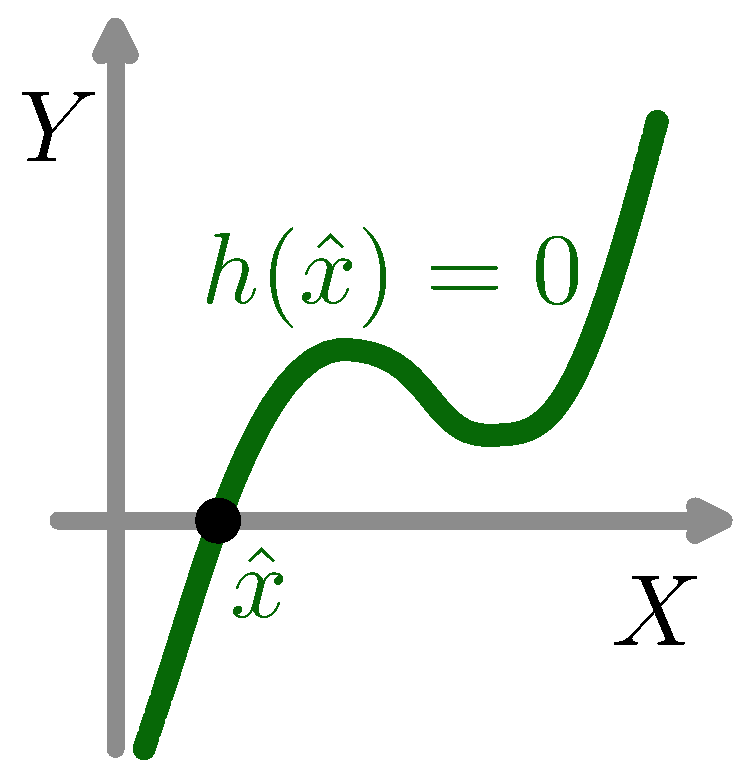
\includegraphics[width=0.95\linewidth]{chapters/roots/roots1.eps} 
\end{minipage}
\begin{minipage}{0.8\textwidth}
Dados,
um escalar $\delta \in \mathbb{R}$, 
um escalar $\alpha \in \mathbb{R}| \alpha>0$, 
um escalar $x \in \mathbb{R}$, 
uma função $h:\mathbb{R} \rightarrow \mathbb{R}$, e 
conhecida a validade da Eq. (\ref{eq:rootshxreg1}),
\begin{equation}\label{eq:rootshxreg1}
0=h(x);
\end{equation}
se desejamos ter o valor $x=\hat{x}$ que cumpra a Eq. (\ref{eq:rootshxreg1})
podemos usar iterativamente a Eq. (\ref{eq:rootshxreg2}),
onde  $h'(x)\equiv \frac{d h(x)}{d x}$,
\end{minipage}

\begin{equation}\label{eq:rootshxreg2}
x_{k} \leftarrow x_{k-1}-\frac{ h'(x_{k-1})h(x_{k-1})}{h'(x_{k-1})^2+\alpha}.
\end{equation}
Assim, $\hat{x}$ pode ser achado\footnote{A 
demostração pode ser vista na Prova \ref{proof:theo:rootshxreg}.} 
iniciando a Eq. (\ref{eq:rootshxreg2}) desde um 
$x_{0}$ qualquer, realizando cálculos $x_{k}$ iterativamente  
ate\footnote{Sendo delta um valor pequeno próximo a zero.} que $||h(x_k)||<\delta$
onde se declara que $\hat{x}=x_k$.

\textbf{Considerações:}
\begin{itemize} 
\item Se $h'(x_{k-1})\approx 0$ indica que estamos perto de um ponto de inflexão 
(máximo, mínimo ou ponto de sela) em $x_{k-1}$. Se neste ponto a Eq. (\ref{eq:rootshxreg2})
converge com valores $x_k\approx x_{k-1}\approx x_{k-2}\approx ...$ e verificamos que $||h(x_{k-1})||>\delta$,
devemos pular aleatoriamente a um novo ponto $x_k$ pois estamos atrapados num mínimo local de $h(x)$.  
\item Uma sugestão do procedimento para a busca de uma raiz pode ser vista no diagrama de fluxo
mostrado na Figura \ref{fig:fluxorhxreg3}. 
\end{itemize}
\end{theorem}

\begin{tcbattention}
\begin{itemize}
\item Uma vantagem do método da regularização em relação ao método de Newton,
é que em lugares onde $h'(x_{k-1})\approx 0$, a regularização converge a um mínimo local 
que facilmente podemos detectar. Em contrapartida,
com o método de newton podemos ficar temporalmente atrapados num mínimo local, porém este estado 
é mais difícil de detectar pois os valores de $x_k$ tendem a divergir para valores próximos ao mínimo.
Esta caraterística pode ser comparada nas Soluções \ref{sol:rootshx1} e \ref{sol:rootshxreg1}
\end{itemize}
\end{tcbattention}

\begin{figure}[!h]
     \centering
         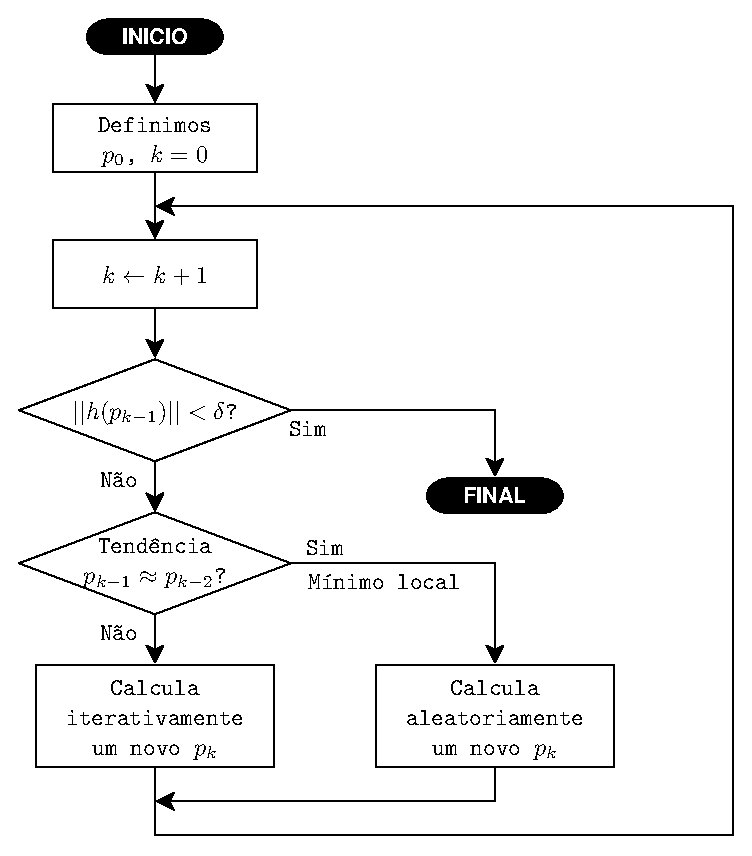
\includegraphics[width=0.75\textwidth]{chapters/roots/fluxo3.eps}
        \caption{Diagrama de fluxo da solução iterativa para achar uma raiz, seguindo o teorema \ref{theo:rootshxreg}.}
        \label{fig:fluxorhxreg3}
\end{figure}

%%%%%%%%%%%%%%%%%%%%%%%%%%%%%%%%%%%%%%%%%%%%%%%%%%%%%%%%%%%%%%%%%%%%%%%%%%%%%%%%
\subsection{Exemplos de busca de raízes pelo método da regularização}


\begin{example}\label{ex:rootshxreg1}
Conhecida uma função $h(x)=x(x^2-1)+1$, e um escalar $\delta=10^{-3}$; usando o Teorema \ref{theo:rootshxreg},
achar o valor $x=\hat{x}$ que cumpra $||h(x)||<\delta$ usando o Teorema \ref{theo:rootshxreg}.
Podemos ver as respostas a este exemplo na Solução \ref{sol:rootshxreg1} e \ref{sol:rootshxreg2}.
\end{example}
\begin{SolutionT}[Relativa ao Exemplo \ref{ex:rootshxreg1} (Converge errado):]\label{sol:rootshxreg1}
 A Fig. \ref{fig:rootsRcasesa} nos mostra o processo de busca das raízes de $h(x)$. 
A busca inicia em $x_0=-0.3$, 
todos os valores $x_{k}$ podem ser vistos na
Tabela \ref{tab:rootsRcases1}. 
Neste caso a busca iterativa indicada pela Eq. (\ref{eq:rootshxreg2}) 
converge em $x_7=0.57812$, que é um valor próximo a $x_m=\frac{\sqrt{3}}{3}\approx 0.57735$,
que é um mínimo local de $h(x)$.
Porém dado que $||h(x_7)||=0.61510 >\delta$, observamos que estamos atrapados num mínimo local,
pelo que devemos fazer um pulo aleatório a um novo valor $x_8$
para tentar fugir deste mínimo local; por exemplo $x_8=-2.0$.
\end{SolutionT}

\begin{figure}[!h]
    \centering
    \begin{subfigure}[b]{0.49\textwidth}
        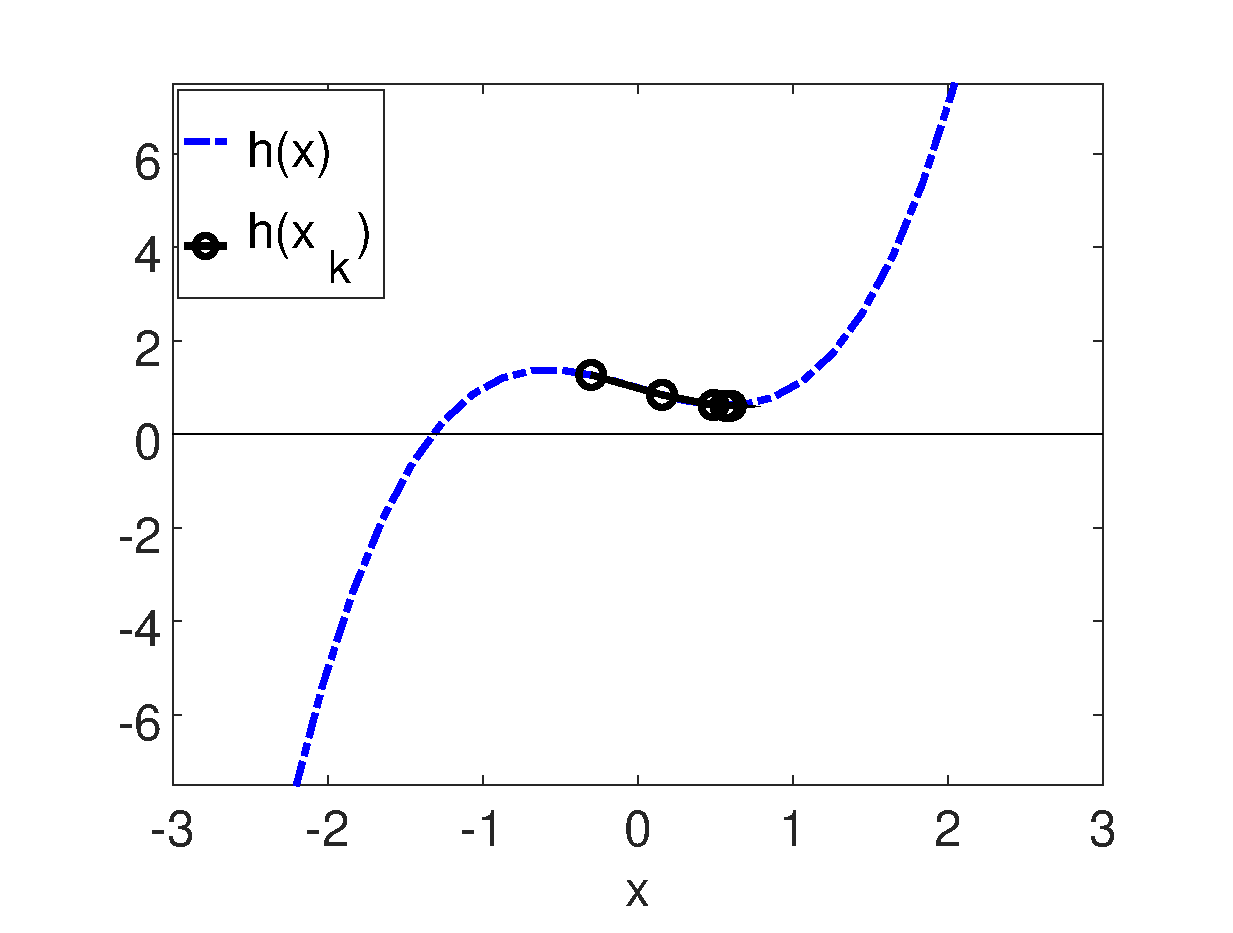
\includegraphics[width=\textwidth]{chapters/roots/mfiles/hx_a/minimizando_hx_a_1.eps}
        \caption{As iterações divergem ao redor de $x_m$, onde $h'(x_m)\approx 0$ e $h(x_m)\neq 0$.}
        \label{fig:rootsRcasesa}
    \end{subfigure}
    ~ %add desired spacing between images, e. g. ~, \quad, \qquad, \hfill etc. 
      %(or a blank line to force the subfigure onto a new line)
    \begin{subfigure}[b]{0.49\textwidth}
        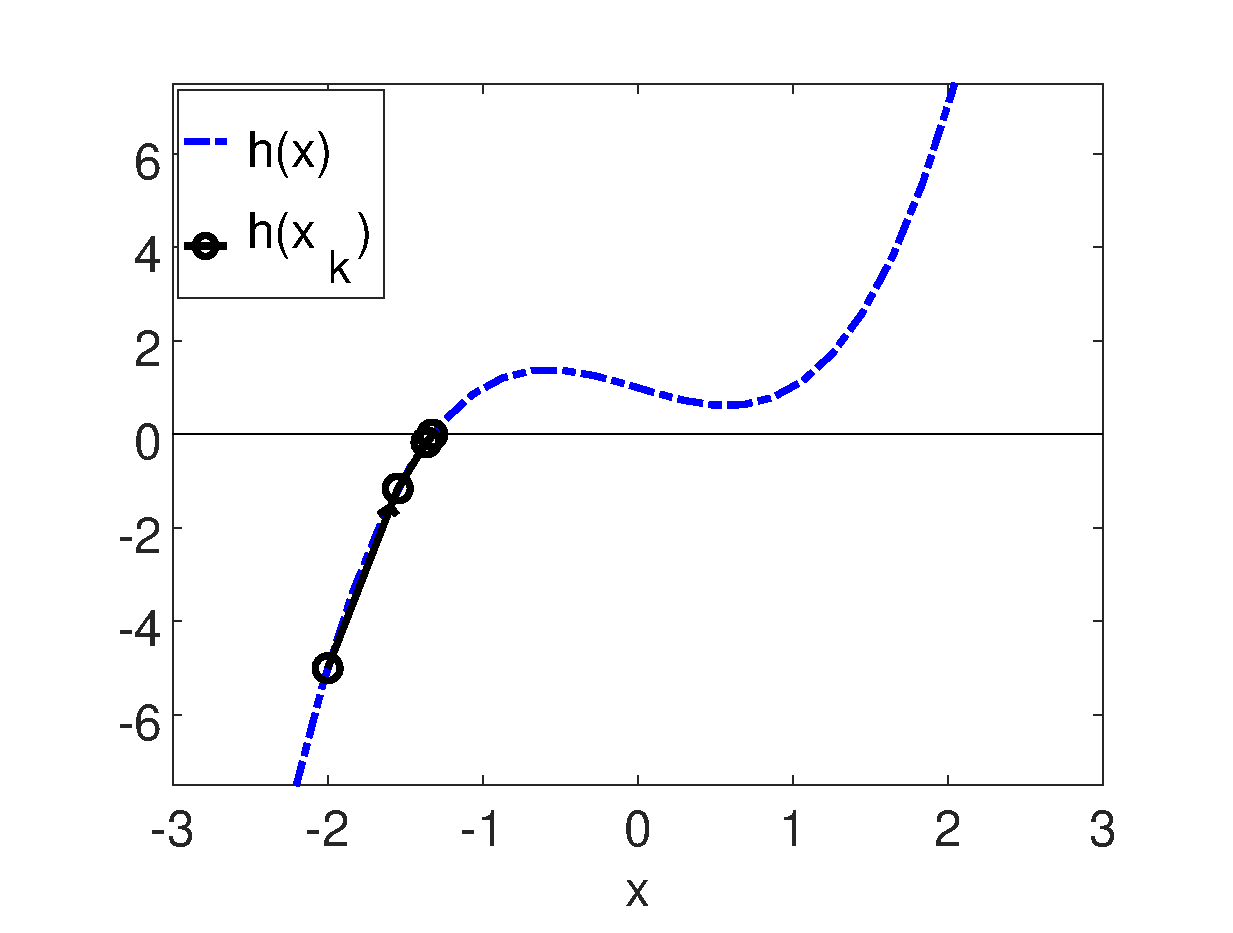
\includegraphics[width=\textwidth]{chapters/roots/mfiles/hx_a/minimizando_hx_a_2.eps}
        \caption{As iterações convergem em $\hat{x}$, onde $h(\hat{x})\approx 0$ e $h'(x_m)\neq 0$}
        \label{fig:rootsRcasesb}
    \end{subfigure}
    \caption{Comportamento da busca iterativa do Exemplo \ref{ex:rootshxreg1}}
    \label{fig:rootsRcases}
\end{figure}

\begin{table}[!h]
\centering
\begin{tabular}{|l|l|l|l|l|l|l|l|l|}
\hline
$k$      & 0 & 1 & 2 & 3 & 4 & 5 & 6 & 7\\ \hline
$x_k$    & -0.30000 & 0.15713 & 0.48972 & 0.60126 & 0.56670 & 0.58168 & 0.57551 & 0.57812 \\ \hline
$||h(x_k)||$ & 1.27300  & 0.84675 & 0.62773 & 0.61610 & 0.61530 & 0.61513 & 0.61511 & 0.61510 \\ \hline
\end{tabular}
\caption{Resposta iterativa do Exemplo \ref{ex:rootshxreg1}.}
\label{tab:rootsRcases1}
\end{table}

\begin{SolutionT}[Relativa ao Exemplo \ref{ex:rootshxreg1} (Converge errado):]\label{sol:rootshxreg2}
A Fig. \ref{fig:rootsRcasesb} nos mostra o processo de busca de uma raiz de $h(x)$. 
A busca inicia em $x_0=-2.0$,
 todos os valores $x_{k}$ podem ser vistos na Tabela \ref{tab:rootsRcases2}. 
Neste caso a busca iterativa indicada pela Eq. (\ref{eq:rootshxreg2}) converge 
em $\hat{x}\approx x_4 = -1.3248$ com $||h(x_4)||<\delta$ que corresponde a uma raiz de $h(x)$.
\end{SolutionT}

\begin{table}[!h]
\centering
\begin{tabular}{|l|l|l|l|l|l|}
\hline
$k$      & 0 & 1 & 2 & 3 & 4 \\ \hline
$x_k$    & -2.0000 & -1.5473 & -1.3626 & -1.3268 & -1.3248 \\ \hline
$||h(x_k)||$ & 5.0000e+00 & 1.1573e+00 & 1.6711e-01 & 9.0760e-03 & 2.5792e-04 \\ \hline
\end{tabular}
\caption{Resposta iterativa do Exemplo \ref{ex:rootshxreg1}.}
\label{tab:rootsRcases2}
\end{table}



\newpage
\section{Provas dos teoremas}
 
%%%%%%%%%%%%%%%%%%%%%%%%%%%%%%%%%%%%%%%%%%%%%%%%%%%%%%%%%%%%%%%%%%%%%%%%%%%%%%%%%%%%%%%
%%%%%%%%%%%%%%%%%%%%%%%%%%%%%%%%%%%%%%%%%%%%%%%%%%%%%%%%%%%%%%%%%%%%%%%%%%%%%%%%%%%%%%%
\begin{myproofT}[Relativa ao Teorema \ref{theo:rootshx}:]\label{proof:theo:rootshx}
Dados
os escalares $\delta \in \mathbb{R}_+$, 
$x \in \mathbb{R}$, 
uma função $h:\mathbb{R} \rightarrow \mathbb{R}$, e 
conhecida a validade da Eq. (\ref{eq:prrof:rootshx1}),
\begin{equation}\label{eq:prrof:rootshx1}
0=h(x);
\end{equation}
se desejarmos ter o valor $x=\hat{x}$ que cumpra que $||h(\hat{x})||<\delta$, 
é aplicado o critério mostrado no Teorema \ref{theo:minhxhx}, no qual se indica que uma forma de achar o 
$x=\hat{x}$ que minimize $e(x)=||h(x)||^2$ é mediante a seguinte equação iterativa.  
\begin{equation}\label{eq:prrof:rootshx1:2}
x_{k}=x_{k-1}-\frac{h(x_{k-1})}{h'(x_{k-1})}.
\end{equation}

\end{myproofT}

\begin{myproofT}[Prova da continuidade de 
$h(x)/h'(x)$:]\label{proof:theo:cont:rootshx}
Conhecida uma função $h(x)$  diferenciável em $x=a$, 
ao menos até a $n$-ésima derivada na qual $h^{(n)}(a)\neq 0$.
Se $h(a)=0$ e $h'(a)=0$ o fator
\begin{equation}\label{eq:prrof:cont1}
F(x)=\frac{h(x)}{h'(x)}
\end{equation}
causa uma indeterminação de zero dividido por zero para $x=a$.
Para resolver esse problema, é aplicada de forma consecutiva a regra de l'Hôpital
sobre a Eq. (\ref{eq:prrof:cont1}); assim podemos afirmar
\begin{equation}\label{eq:prrof:cont2}
F(a)=\lim_{x\rightarrow a}\frac{h(x)}{h'(x)}=\frac{h^{(n-1)}(a)}{h^{(n)}(a)},
\end{equation}
sendo que $n$ é escolhido como o primeiro valor avaliado em $a$, 
no qual se cumpra que $h^{(n)}(a)\neq 0$. 
Assim, podemos definir que os lugares onde $h(a)=0$ e $h'(a)=0$,
 também tem um valor $F(a)\neq 0$,
se $h(x)$ tem ao menos uma derivada $n$-ésima em $x=a$ que provoque $h^{(n)}(a)\neq 0$.

Uma forma simples de expressar isso é indicar que $F(a)\neq 0$, se é possível
expressar $h(x)$ em \hyperref[def:taylor]{\textbf{série de Taylor}} ao redor de $x=a$. 
\end{myproofT}

%%%%%%%%%%%%%%%%%%%%%%%%%%%%%%%%%%%%%%%%%%%%%%%%%%%%%%%%%%%%%%%%%%%%%%%%%%%%%%%%%%%%%%%
%%%%%%%%%%%%%%%%%%%%%%%%%%%%%%%%%%%%%%%%%%%%%%%%%%%%%%%%%%%%%%%%%%%%%%%%%%%%%%%%%%%%%%%
\begin{myproofT}[Relativa ao Teorema \ref{theo:rootshxreg}:]\label{proof:theo:rootshxreg}
Dados
os escalares $\delta \in \mathbb{R}_+$,
$\alpha \in \mathbb{R}_+$, 
$x \in \mathbb{R}$, 
uma função $h:\mathbb{R} \rightarrow \mathbb{R}$, e 
conhecida a validade da Eq. (\ref{eq:prrof:rootshxreg1}),
\begin{equation}\label{eq:prrof:rootshxreg1}
0=h(x);
\end{equation}
se desejarmos ter o valor $x=\hat{x}$ que cumpra que $||h(\hat{x})||<\delta$, 
é aplicado o critério mostrado no Teorema \ref{theo:minhxhxxoxo},
em que se indica que uma forma de achar o valor 
$x=\hat{x}$ que minimiza $e(x)=||h(x)||^2+\alpha||x-x_{last}||^2$, 
é mediante a seguinte equação iterativa,  
\begin{equation}\label{eq:prrof:rootshxreg1:2}
x_{k}=x_{k-1}-\frac{h'(x_{k-1}) h(x_{k-1})}{h'(x_{k-1})^2+\alpha};
\end{equation}
na qual $\alpha$ é um multiplicador de Lagrange escolhido por nós.

A Eq. (\ref{eq:prrof:rootshxreg1:2}) tenta minimizar simultaneamente 
as funções de custo $||h(x)||^2$ 
e $||x-x_{last}||^2$, para nos aproximar a Eq. (\ref{eq:prrof:rootshxreg1});
a busca iterativa acha a convergência quando obtém valores $x_{k}\approx x_{k-1}$;
porém esta pode acontecer quando achamos um mínimo local ou global;
por isso, é importante verificar se $||h(x)||<\delta$. 
\end{myproofT}


%% Metodo de newton modificado
%% https://books.google.com.br/books?id=5XappvcENCMC&pg=PA65&dq=roots+%2B+newton+%2B+raphson+%2B+modified&hl=pt-BR&sa=X&ved=0ahUKEwjIvIaB7r_mAhUAHLkGHVZtBf8Q6AEIKTAA#v=onepage&q=roots%20%2B%20newton%20%2B%20raphson%20%2B%20modified&f=false




%----------------------------------------------------------------------------------------
%	BIBLIOGRAPHY
%----------------------------------------------------------------------------------------

\chapter*{Bibliografia}
\addcontentsline{toc}{chapter}{\textcolor{ocre}{Bibliography}}
\section*{Miscelânea}
\addcontentsline{toc}{section}{Miscelânea}
\printbibliography[heading=bibempty,type=misc]
\section*{Livros}
\addcontentsline{toc}{section}{Livros}
\printbibliography[heading=bibempty,type=book]
\section*{Artigos}
\addcontentsline{toc}{section}{Artigos}
\printbibliography[heading=bibempty,type=article]

%----------------------------------------------------------------------------------------
%	INDEX
%----------------------------------------------------------------------------------------

\cleardoublepage
\phantomsection
\setlength{\columnsep}{0.75cm}
\addcontentsline{toc}{chapter}{\textcolor{ocre}{Index}}
\printindex

%----------------------------------------------------------------------------------------

\end{document}
